\documentclass[8pt]{beamer}
%\usetheme{Warsaw}
%\usecolortheme{spruce}
\usetheme{CambridgeUS}
% \usefonttheme[onlymath]{serif}
\usecolortheme{dolphin}
\mode<presentation>{}

\usepackage{empheq}
\usepackage{url}

\usepackage{array}
\usepackage{amsmath, amsfonts, bm}

\usepackage[many]{tcolorbox}
\newtcbox{\mymath}[1][]{%
    nobeforeafter, width=\textwidth, math upper, enhanced, 
    colframe=gray!10!white, boxrule=0pt, arc=1mm, outer arc=1mm, opacityback=0.5,
    frame hidden, borderline={0.5pt}{0pt}{gray!20!white},
    #1}

% Change example block width
\addtobeamertemplate{block example begin}{%
    \setlength{\textwidth}{0.8\textwidth}
}{}

\usepackage{booktabs}

\usepackage{amsmath, amssymb, amsthm} % *** MATH PACKAGES ***
% \setbeamertemplate{blocks}[rounded][shadow=true]
\usepackage{tcolorbox}
\usepackage{mathtools}
\usepackage{tcolorbox} % For colored boxes
\usepackage{empheq} % Extended equation environments
%\usepackage{enumitem}

\usepackage{minted}

%----------------------------
%References
\usepackage[style=ieee]{biblatex} % You can choose different styles
\addbibresource{References.bib} % Add the .bib file

\usepackage{framed, color}
%% preamble
\title{\textbf{Introduction to Kalman Filter}}
%\subtitle{\textbf{Lecture 3 \& 4}}
\author[Aamir Mahmood]{Aamir Mahmood \\ \footnotesize aamir.mahmood@miun.se}
\institute[]{Mid Sweden University}
\titlegraphic{
\includegraphics[width=0.15\textwidth]{Figures/mittuniversitetet_logo.png}}
\date{\today}
\begin{document}

%% title frame
\begin{frame}

\titlepage
\end{frame}

\section*{Acknowledgments}
\begin{frame}{Acknowledgments}
    \begin{itemize}
        \item The lecture slides are mainly based on the book, \textit{Kalman Filter from the Ground Up} by \textit{Alex Becker}.
        
        \item The figures in these slides are primarily sourced from \textit{Kalman Filter
        from the Ground Up}, except for those generated from my own implementation of the codes.
        \item The codes and the results generated are my own contributions and were developed specifically for these lecture slides.
        \item Additional information in the slides has been compiled from various sources.
        %, including [mention key sources, if any].
        \item All rights to the original figures and content remain with the original authors and publishers.
    \end{itemize}
\end{frame}
%-----------------------------------------------------
\begin{frame}[allowframebreaks]
   \frametitle{Outline}
		\tableofcontents
\end{frame}

%-----------------------------------------------------

\section{About Kalman and The Filter}

\subsection{On Rudolf E. Kalman}
\begin{frame}
   \frametitle{On Rudolf E. Kalman}

		\begin{itemize}
			\item Born in Budapest, Hungary, May 19, 1930
			\item Passed away in Gainsville, Florida, July 2, 2016
			\item Emigrated to USA in 1943
			\item Bachelor and Master in EE at MIT, 1953 and 1954, respectively
			\item Ph.D. at Columbia University, 1957 (Advisor: J. R. Ragazzini)
			\item Institutions: Stanford University, University of Floria, ETC Zurich (and more)
		\end{itemize}
		
		\begin{figure}
		\centering
			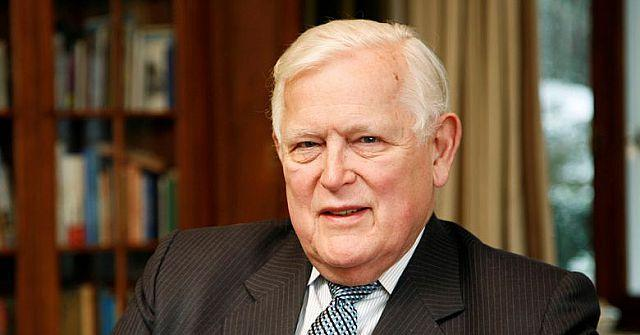
\includegraphics[width=0.70\textwidth]{Figures/Background/R. E. Kalman.jpg}
		\label{fig:REKalman}
		\caption{Rudolf E. Kalman}
	\end{figure}
	This is where it all started: \cite{Henrik_KF}	
\end{frame}
%-----------------------------------------------------

\subsection{The Filter}
\begin{frame}
   \frametitle{The Filter}
		\begin{itemize}
			\item The filter invented by R. E. Kalman in the 1960s, based on the seminal papers:
			    \begin{enumerate}
			        \item R. E. Kalman: Contribution to the Theory of Optimal Control (1960)
			        \item \textbf{R. E. Kalman: A New Approach to Linear Filtering and Prediction Problems (1960)}
			        \item R. E. Kalman: Mathematical Description of Linear Dynamical Systems (1963)
			    \end{enumerate}
			\item (2) describes a recursive solution to the discrete-data linear filtering problem---Kalman Filter
			
			\item Enormous impact on the fields of \textbf{linear systems theory, statistics, signal processing, identification, feedback control, and adaptive systems}
			
			\item Additionally, on motivating new formulations of feasible filtering problems outside the linear domain. 
			
			\item Kalman Filtering is used extensively, mainly for \textit{target tracking}. However, it can be applied to any field where \textit{estimation and prediction} are required, e.g., location and navigation systems, control systems, computer graphics, and much more.
		\end{itemize}
		
		\vspace{10pt}
		\textbf{Estimation problem}: Estimating hidden (unknown) states based on a series of measurements.
		
		\begin{itemize}
		    \item For example, a GPS receiver provides location and velocity estimation, where location and velocity are the hidden states and differential time of the satellites' signals' arrival are the measurements.
		    \item Challenge is providing an accurate and precise estimation of the hidden states in the \textbf{presence of uncertainty}.
		    \begin{itemize}
		        \item In GPS receivers, the measurement uncertainty depends on many external factors such as thermal noise, atmospheric effects, slight changes in satellite positions, receiver clock precision, etc.
		    \end{itemize}
		   \item The Kalman Filter produces estimates of hidden variables based on inaccurate and uncertain measurements.  
		\end{itemize}
		
		
\end{frame}
%-----------------------------------------------------
\begin{frame}
   \frametitle{Filtering}
   
   Estimate the current value of the stochastic signal, using the history and current value of another observed stochastic process; e.g., using the measurements $Y_k = \{y_i, i\leq k\}$, we want to estimate $\hat{x}_{k + m}$. It leads to three cases:
   	\begin{figure}
		\centering
			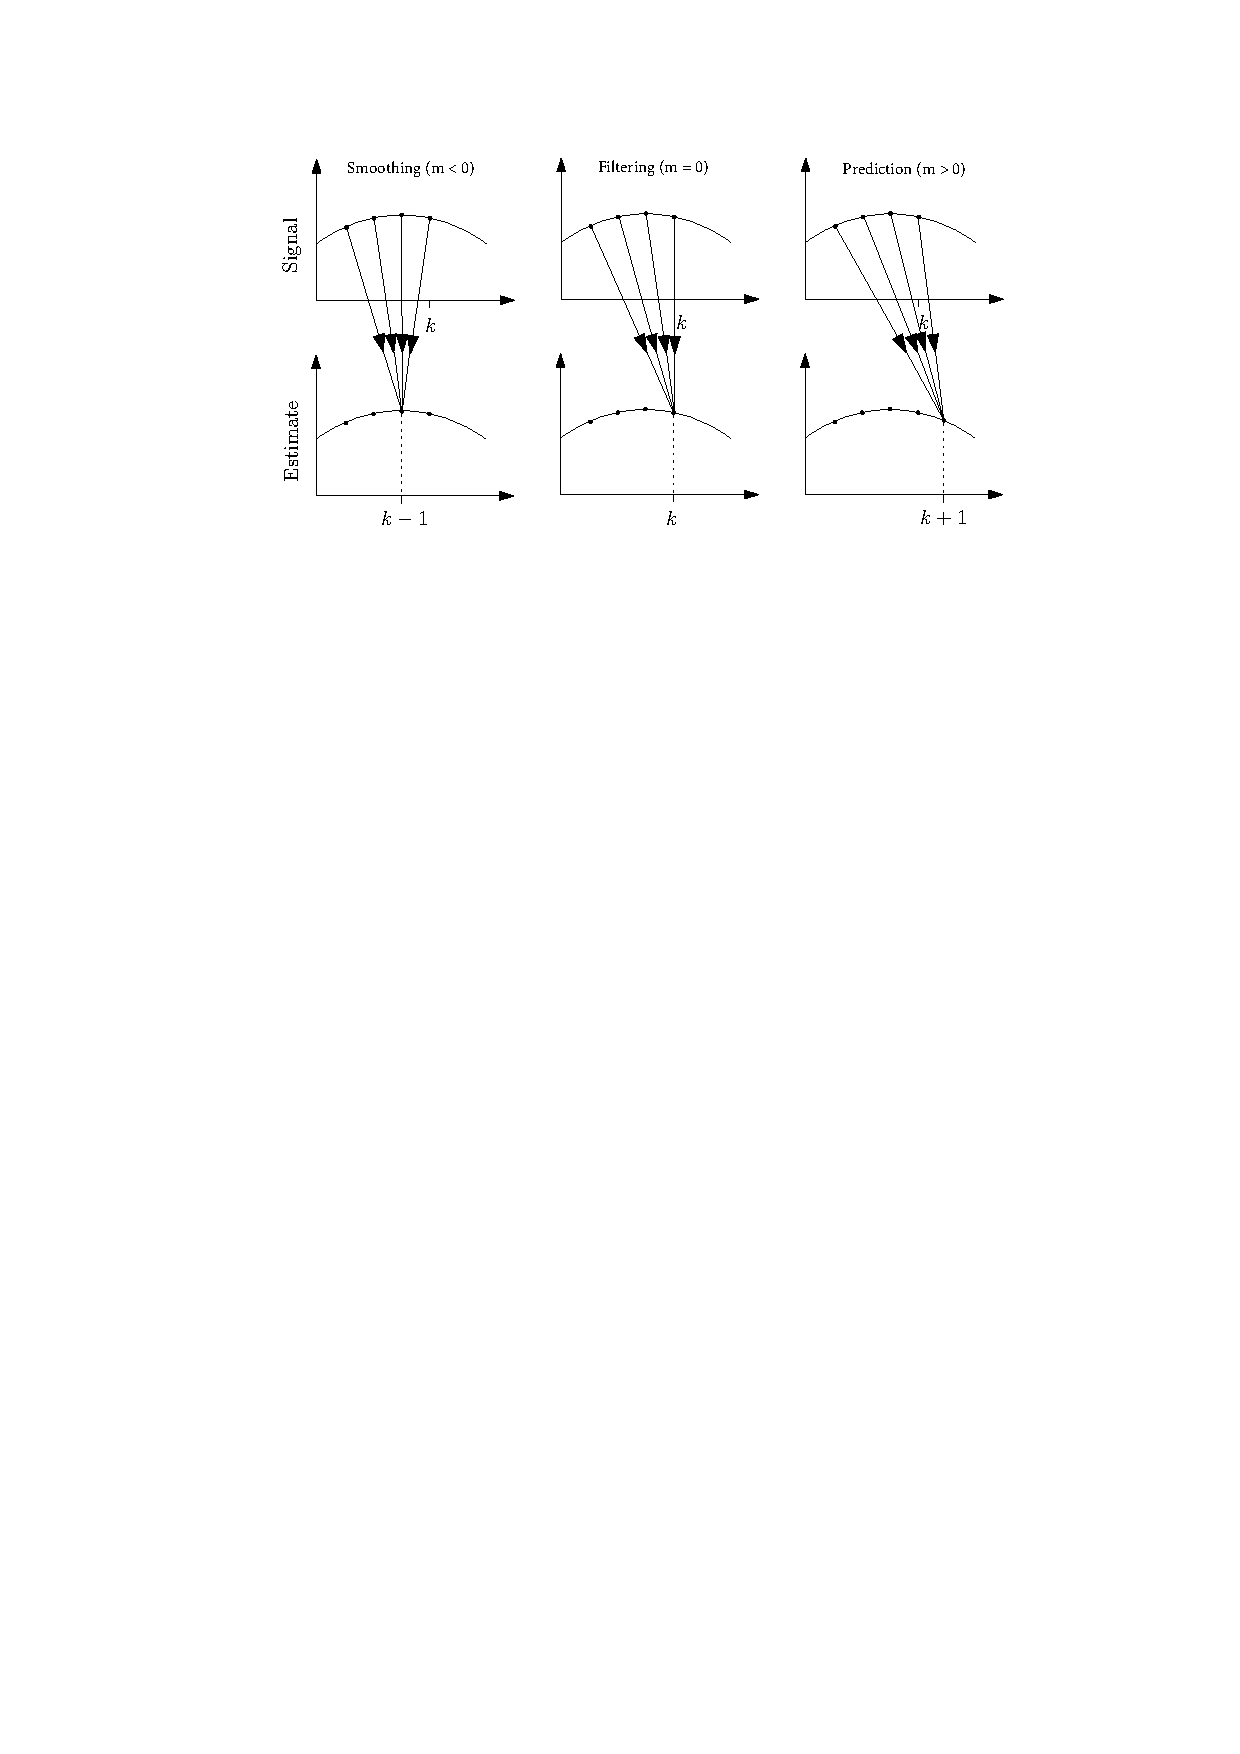
\includegraphics[width=0.70\textwidth]{Figures/Background/Smoothing, Filtering, and Prediction.pdf}
		\label{fig:WirelessVision}
		\caption{Smoothing, filtering, prediction}
	\end{figure}
	\begin{itemize}
	    \item \textbf{Smoothing}: Estimation of the past state-variable at the present time
	    \item \textbf{Filtering}: Estimating the present state-variable at the present time
	    \item \textbf{Prediction}: Estimating the future state-variable at the present time
	\end{itemize}

\end{frame}


\begin{frame}\frametitle{The Necessity of Prediction}
   
   \textbf{Radar tracking algorithm}
    
    \begin{columns}\column{0.5\textwidth}
        
    \begin{itemize}
        \item The tracking radar sends a pencil beam in the direction of the target.
        \item In every track cycle of $\Delta t$, the radar revisits the target by sending a dedicated track beam in the direction of the target.    
        \item After sending the beam, the radar estimates the current target position and velocity. The radar also estimates (or predicts) the target position at the next track beam.
    \end{itemize}
    \begin{figure}
		\centering
			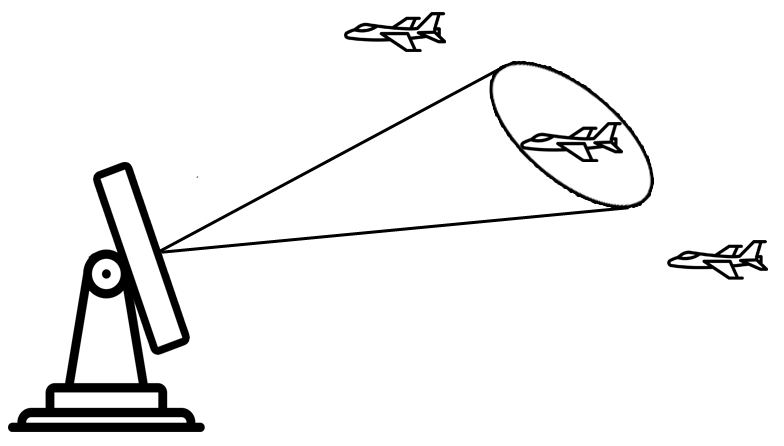
\includegraphics[width=0.8\textwidth]{Figures/Background/tracking_radar.png}
		\label{fig:Radar_Tracking}
	\end{figure} 
        
    \column{0.5\textwidth}
    \vspace{-15pt}
    \begin{itemize}
        \item The future target position can be easily calculated using Newton's motion equations:
        \vspace{-8pt}
        $$x = x_0 + v_0 \Delta t + \frac{1}{2}a\Delta t^2$$
        where\\ 
        $x$~~~is the target's position\\
        $x_0$~~is the target's initial position\\
        $v_0$~~is the target's initial velocity\\
        $a$~~~is the target's acceleration\\
        $\Delta t$ is the track cycle\\
    \end{itemize}
    
    In 3D, it can be written as a system of equations
    \begin{align*}
     x = & x_0 + v_{x0} \Delta t + \frac{1}{2}a_x\Delta t^2\\\nonumber
     y = & y_0 + v_{y0} \Delta t + \frac{1}{2}a_y\Delta t^2\\\nonumber
     z = & z_0 + v_{z0} \Delta t + \frac{1}{2}a_z\Delta t^2\\\nonumber
    \end{align*}
    \end{columns}
   The above set of equations is called a \textbf{Dynamic Model} (or a \textbf{State Space Model}). The Dynamic Model describes the relationship between input and output.
\end{frame}

%-----------------------------------------------------
\begin{frame}{Constant Acceleration}
    \begin{figure}
		\centering
			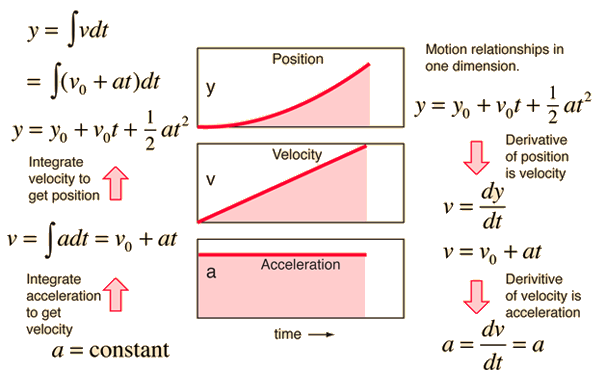
\includegraphics[width=0.7\textwidth]{Figures/Background/Constant Acceleration.png}
		\label{fig:Radar_Tracking}
	\end{figure}     
    
\end{frame}

%-----------------------------------------------------
\begin{frame}{Terminologies using tracking example}
    
    
    \begin{itemize}
    
        \item \textbf{Dynamic or State Space Model:} Describes the relationship between input and output. 
        \item \textbf{System State}
    
            \begin{itemize}
                \item The target parameters $[x, y, z, v_x, v_y, v_z, a_x, a_y, a_z]$ are called a \textbf{System State}. 
                
                \item The current state is the input to the prediction algorithm and the next state (the target parameters at the next time interval) is the algorithm's output.
            \end{itemize}
    
        \item So, if the current state and the dynamic model are known, the next target state can be easily predicted? \textbf{Well, not really!}
        
        \item \textbf{Measurement Noise:} The radar measurement is not absolute; it includes a random error (or uncertainty). The error magnitude depends on many parameters, such as radar calibration, the beam width, and the signal-to-noise ratio of the returned echo. \textit{The error included in the measurement is called Measurement Noise.}
        
        
        \item \textbf{Process Noise:} The target motion is not strictly aligned to motion equations due to external factors such as wind, air turbulence, and pilot maneuvers. \textit{The dynamic model error (or uncertainty) is called Process Noise.}
    \end{itemize}
    
    \begin{framed}
    Due to Measurement Noise and Process Noise, the estimated target position can be far away from the actual target position. In this case, the radar might send the track beam in the wrong direction and miss the target.
    \end{framed}
    
\end{frame}

%-----------------------------------------------------



\section{Part 1: The Kalman Filter for Dummies}
\begin{frame}
   \frametitle{Part 1: The Kalman Filter for Dummies}
		
		\textbf{Objectives}
				
		\begin{itemize}
			\item Understand the concept of the Kalman Filter and develop “Kalman Filter intuition”
			\item Being able to design a one-dimensional Kalman Filter
			\item \textit{While}, developing necessary mathematical background using practical numerical examples with easy and intuitive explanations
		\end{itemize}
		
		\vspace{10pt}
		
		\begin{exampleblock}{}
  {\small ``The road to learning by precept is long, by example short and effective.''}
  \vskip3mm
  \hspace*\fill{\small--- Lucius Seneca}
\end{exampleblock}


% 		\begin{framed}
% 		\begin{center}
% 		\textbf{Designing reliable systems with guaranteed performance under time dependent varying wireless channel chracteristics }
% 		\end{center}
% 		\end{framed}
\end{frame}

%------------------------------------------------------------
\subsection{Essential Background}

\begin{frame}{Mean and Expected Value // Variance and Standard Deviation}

\begin{itemize}
    \item \textbf{Mean ($\mu$):} Find mean of 5 coins, e.g., $V_{\text{mean}} = \frac{1}{N}\sum_1^N V_n = \frac{1}{5}  (5+5+10+10+10)=8\,\text{cent}$ (no hidden system states)
    \item \textbf{Expected value ($E$)}: The expected value is the value you would expect your hidden variable to have over a long time or many trials. Example: Different weight measurements of the same person.
    \begin{itemize}
        \item Person is the system, person's weight is the system state.
        \item The measurements will be different due to random measurement errors of the scale.
        \item True weight is unknown since it is a \textbf{Hidden State}. To estimate the weight: $W = \frac{1}{N}\sum_1^N W_n$
    \end{itemize}

    \item \textbf{Variance ($\sigma^2$):} is a measure of the spreading of the data set from its mean. $$\sigma^2 = \frac{1}{N}\sum_1^N (x_n-\mu)^2$$
    \item \textbf{Standard deviation ($\sigma$)} is the square root of the variance. 

    \item When estimating variance, with factor $N-1$ is called Bessel's correction:
    $$\sigma^2 = \frac{1}{N-1}\sum_1^N (x_n-\mu)^2$$
    See proof at   \href{https://www.visiondummy.com/2014/03/divide-variance-n-1/}{\textcolor{blue}{visiondummy}}.
    
      
\end{itemize}


\end{frame}


\begin{frame}{Estimation, Accuracy, Precision}
    % \begin{columns}
        %  \column{0.5\textwidth}  
        \begin{itemize}
            \item \textbf{Estimate:} Evaluating the hidden state (e.g., aircraft's true position) using sensor(s) (i.e., radar) measurements
            \item \textbf{Accuracy:} indicates how close the measurement or estimate is to the true value
            \item \textbf{Precision} describes the variability of measurements or estimate of the parameter of interest
            
            \begin{figure}
		       \centering
		        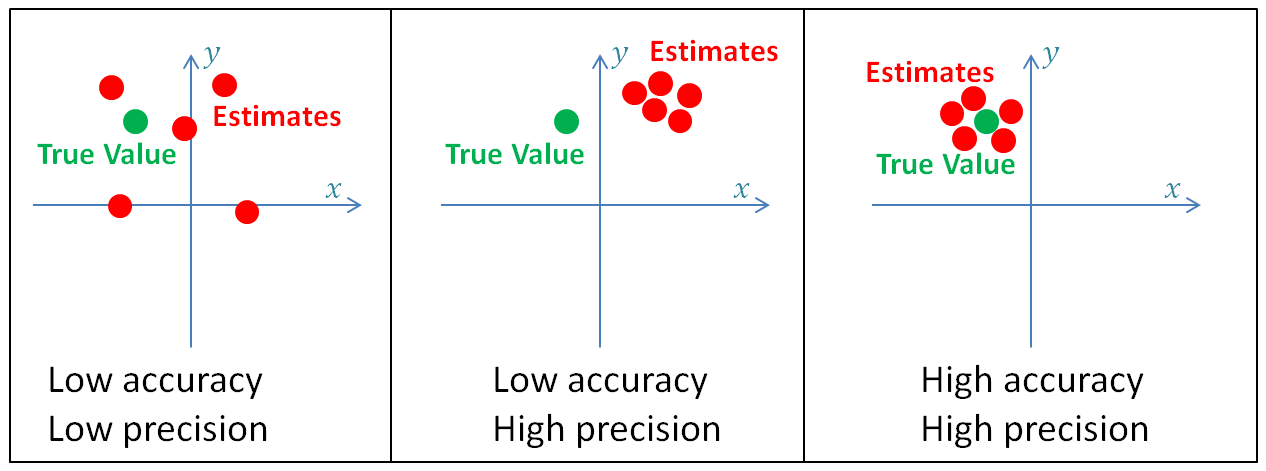
\includegraphics[width=0.7\textwidth]{Figures/Chapter1/AccuracyAndPrecision.png}
		        \label{fig:AccuracyAndPrecision}
	        \end{figure}
	        High-precision systems have low variance in their measurements (i.e., low uncertainty) and vice versa. \textit{The random measurement error produces the variance.}
	        
	        Q: How to reduce the influence of variance (A: Averaging or smoothing)
	        
	        \vspace{5pt}
	        While, low-accuracy systems are called \textbf{biased} systems as their measurements have a built-in systematic error or bias. \textit{A biased thermometer will produce a constant systematic error in the estimate.}
	        
	        
        \end{itemize} 
        %  \column{0.5\textwidth}
    % \end{columns}
\end{frame}


%-----------------------------------------------------
\begin{frame}{Estimation, Accuracy, Precision: Summary}
            \begin{figure}
		       \centering
		        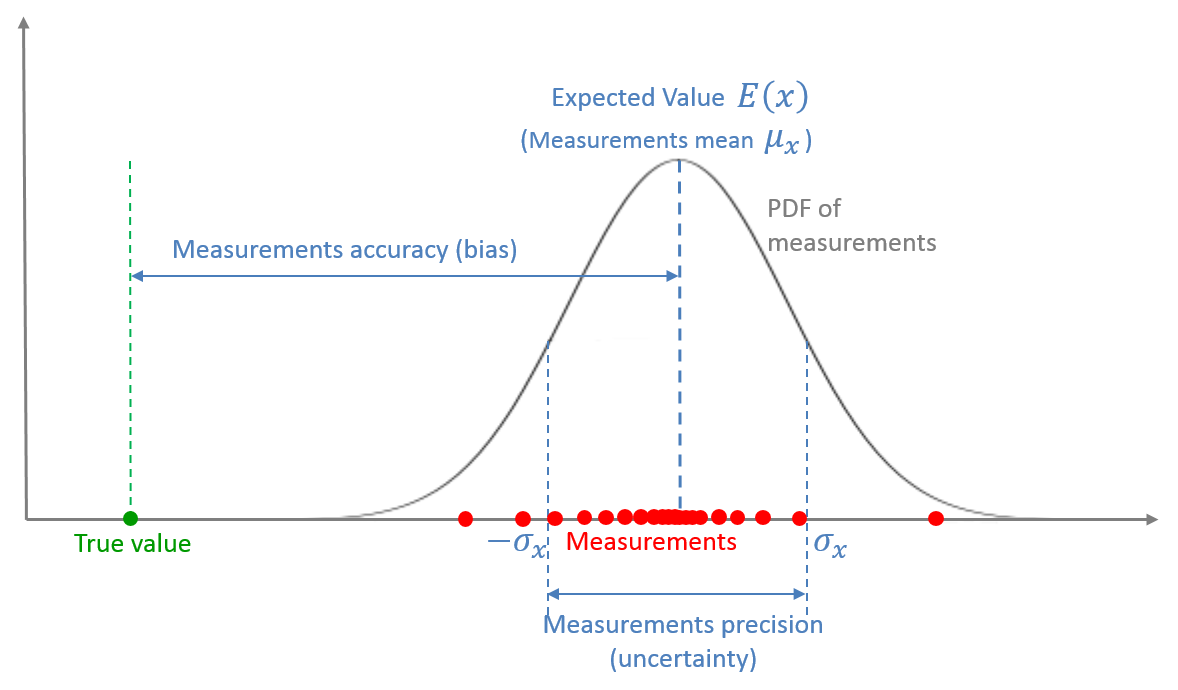
\includegraphics[width=0.65\textwidth]{Figures/Chapter1/statistical_view.png}
		        \label{fig:statistical_view}
	        \end{figure}
    
    The offset between the measurement's mean and the true value is the \textcolor{blue}{measurement's accuracy}, also known as \textcolor{blue}{bias} or \textcolor{blue}{systematic measurement error}.
    
    \vspace{5pt}
    The dispersion of the distribution is the measurement precision, also known as the \textcolor{blue}{measurement noise}, \textcolor{blue}{random measurement error}, or \textcolor{blue}{measurement uncertainty}.
\end{frame}
%-----------------------------------------------------
\subsection{$\alpha-\beta-\gamma$ Filter}

\begin{frame}{$\alpha-\beta-\gamma$ Filter}
Introduction to $\alpha - \beta$ and $\alpha - \beta - \gamma$ filters, which are frequently used for time series data smoothing. The principles of $\alpha - \beta (- \gamma)$ are closely related to Kalman Filter principles.

\end{frame}


\subsubsection{Example~1: Weighting the Gold (A Static System)}
\begin{frame}{Example~1: Weighting the Gold (A Static System)}
    \textbf{Objective: Estimate static system's state, e.g., estimate a gold bar's weight}\\
    \begin{itemize}
        \item The scale is unbiased---the measurements don't have a systematic error but the random noise.
        \item The system's dynamic model is constant, i.e., $\boxed{\hat{x}_{n+1,n} = \hat{x}_{n,n}}$
        \item To estimate the system's state (i.e., the weight value), we can take multiple measurements and average them. 
        \item At the time $n$, the estimate $\hat{x}_{n,n}$ is
        $$\hat{x}_{n,n} = \frac{1}{n}\sum_{i=1}^n z_i$$
    \end{itemize}
        \textit{Example notations:}\\ 
        $x$~~~~~~~~~~is the true value of the weight\\
        $z_n$~~~~~~~~~is the measured value of the weight at time $n$\\
        $\hat{x}_{n,n}$~~~~~~~is the estimate of $x$ at time $n$ (the estimate is made after taking the measurement $z_n$)\\
        $\hat{x}_{n+1,n}$~~~~is the estimate of the future state $(n+1)$ of $x$. The estimate is made at the time $n$. \\~~~~~~~~~~~~In other words, $\hat{x}_{n+1,n}$ is a predicted state or extrapolated state\\
        $\hat{x}_{n-1,n-1}$ is the estimate of $x$ at time $n-1$ (the estimate is made after taking measurement $z_{n-1}$)\\
        $\hat{x}_{n,n-1}$~~~~is the previous prediction---estimate of the state at time $n$, made at time $n-1$\\
\end{frame}
%-----------------------------------------------------
\begin{frame}{State Update Equation}

It is more practical to keep the last estimate only $(\hat{x}_{n-1,n-1})$ and update it after every new measurement.
        \begin{figure}
		    \centering
		    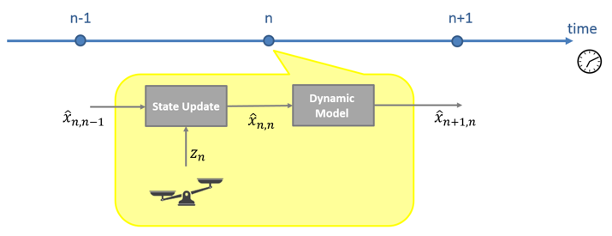
\includegraphics[width=0.7\textwidth]{Figures/Chapter1/ex1_stateupdateequation.png}
		    \label{fig:ex1_stateUpdate}
	    \end{figure}

    \begin{itemize}
        \item Estimate the current state based on the measurement and prior prediction.
        \item Predict the next state based on the current state estimate using the Dynamic Model.
    \end{itemize} 

\end{frame}

\begin{frame}{State Update Equation}
    \begin{columns}
        \column{0.5\textwidth}
        \begin{align*}
            \hat{x}_{n,n} & =  \frac{1}{n}\sum_{i=1}^n z_i \\
                          & =  \frac{1}{n}\left(\sum_{i=1}^{n-1} z_i +z_n \right)\\   
                          & = \frac{n-1}{n}\left(\frac{1}{n-1} \sum_{i=1}^{n-1} z_i\right) +\frac{1}{n}z_n\\
                          & = \hat{x}_{n-1,n-1} - \frac{1}{n} \hat{x}_{n-1,n-1} +\frac{1}{n}z_n\\
                          & = \hat{x}_{n-1,n-1} + \frac{1}{n} \left(z_n - \hat{x}_{n-1,n-1} \right)
        \end{align*}
        
        Using the system's dynamic model, we can extrapolate $\hat{x}_{n-1,n-1}$ to predict the state of $x$ at the time $n$, i.e., $\hat{x}_{n,n-1}$. For a static system, we have \textcolor{blue}{$\hat{x}_{n,n-1}= \hat{x}_{n-1,n-1}$}. Thus, 
        \vspace{-5pt}
        \begin{equation}
            \boxed{\hat{x}_{n,n} = \hat{x}_{n,n-1} + \frac{1}{n} \left(z_n - \hat{x}_{n,n-1}\right)}
        \end{equation}
        
        \column{0.5\textwidth}
        
        Eq. (1) is one of the five Kalman Filter equations, called as \textcolor{blue}{State Update Equation}, and described as
        \begin{figure}
		    \centering
		    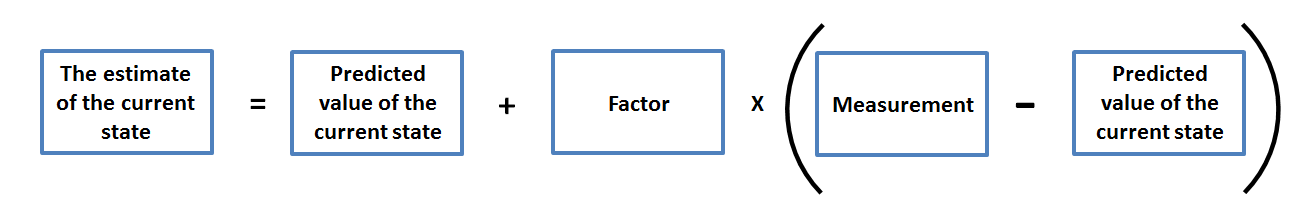
\includegraphics[width=1\textwidth]{Figures/Chapter1/ex1_stateUpdate.png}
		    \label{fig:ex1_stateUpdate}
	    \end{figure}
        
        \begin{itemize}
            \item In Kalman Filter, the factor $\frac{1}{n}$ (specific to this example) is called as \textcolor{blue}{Kalman Gain}, denoted by $K_n$.
            \item The term $\left(z_n - \hat{x}_{n,n-1}\right)$ is the measurement residual, also called as the \textcolor{blue}{INNOVATION} (containing new information).
            
            \item $1/n$ decreases as $n$ increases $\rightarrow$ each successive measurement has less weight in the estimation process.
            
            \item Using $\alpha_n = 1/n$ in our example,
            \vspace{-3pt}
            $$\hat{x}_{n,n} = \hat{x}_{n,n-1} + \alpha_n \left(z_n - \hat{x}_{n,n-1}\right)$$
        \end{itemize}
    \end{columns}
\end{frame}
%-----------------------------------------------------
\begin{frame}{Estimation Algorithm in Example~1}
        \begin{figure}
		    \centering
		    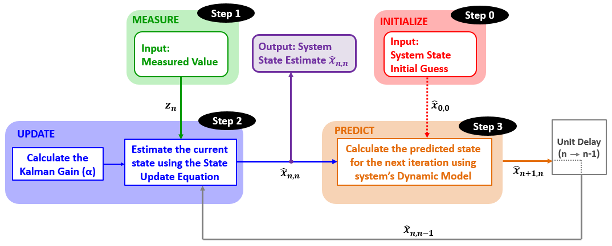
\includegraphics[width=0.7\textwidth]{Figures/Chapter1/ex1_estimationAlgorithm.png}
		    \label{fig:ex1_estimationAlgorithm}
            \caption{State Update Equation.}
	    \end{figure}
	\textbf{Iteration Zero}    
	\begin{itemize}
	    \item \textbf{Initialization:} We start by making a guess or rough estimate of the gold bar weight. It is called the \textcolor{blue}{Initial Guess} for the filter initialization.
	    $$\hat{x}_{0,0} = 1000\,g$$
	    \item \textbf{Prediction:} As the dynamic model of the system is static, our next state estimate (prediction) equals initialization, i.e., 
	    $$\hat{x}_{1,0}=\hat{x}_{0,0} = 1000\,g$$
	\end{itemize}        
\end{frame}
%-----------------------------------------------------
\begin{frame}{Estimation Algorithm in Example~1}
\begin{columns}
    \column{0.5\textwidth}
    \textbf{Iteration 1}
    \begin{itemize}
        \item \textbf{Step~1:} Making the weight measurement
        $$z_1 = 1030 g$$
        \item \textbf{Step~2:}\\
        Calculating the gain from $\alpha_n = 1/n$
        $$\alpha_1 = 1/1 = 1$$
        Calculating the current estimate using the State Update Equation
        $$\hat{x}_{1,1} = \hat{x}_{1,0} + \alpha_1 \left(z_1 - \hat{x}_{1,0}\right) = 1030g$$
        \item \textbf{Step~3:} The dynamic model of the system is static; thus, our next state estimate (prediction) equals to current state estimate
        $$\hat{x}_{2,1}=\hat{x}_{1,1} = 1030g$$
     \end{itemize}
\column{0.5\textwidth}    
\textbf{Iteration 2}
\begin{itemize}
    \item After a unit time delay, the predicted estimate from the previous iteration becomes the prior estimate in the current iteration
    $$\hat{x}_{2,1}= 1030g$$
    \item \textbf{Step~1:} Making the second measurement of the weight
    $$z_2= 989g$$
    \item \textbf{Step~2:} \\
    Calculating the gain
    $$\alpha_2= 1/2$$
    Calculating the current estimate:
    $$\hat{x}_{2,2} = \hat{x}_{2,1} + \alpha_2 \left(z_2 - \hat{x}_{2,1}\right) = 1009.5g$$
    \item \textbf{Step~3:} 
    $$\hat{x}_{3,2} = \hat{x}_{2,2} = 1009.5$$
\end{itemize}
\end{columns}
\end{frame}
%-----------------------------------------------------
\begin{frame}{Example~1: Results}
        \begin{figure}
		    \centering
		    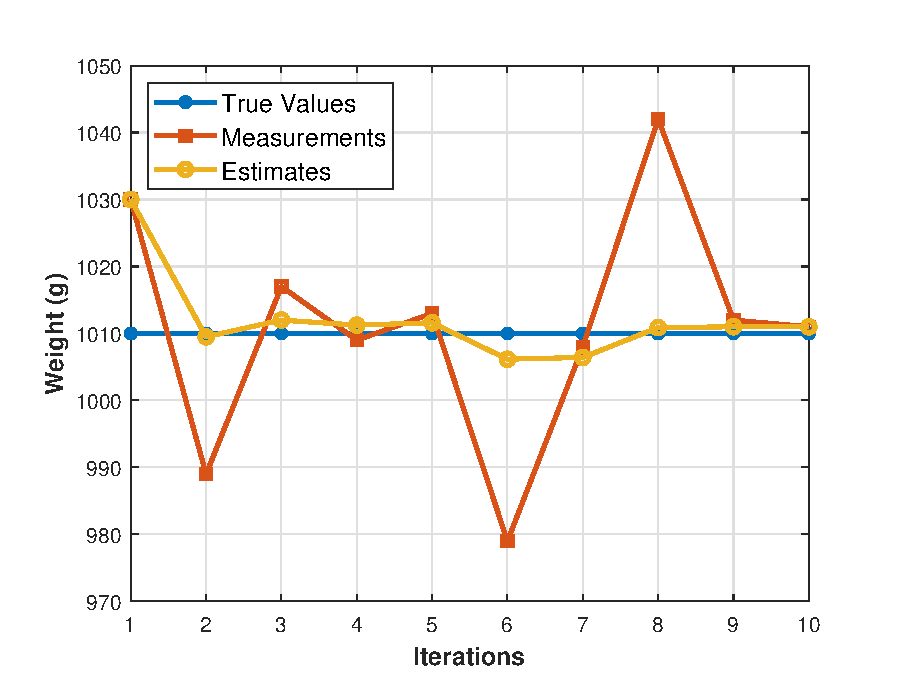
\includegraphics[width=0.6\textwidth]{Figures/Chapter1/ex1_estimationAlgorithm.eps}
		    \label{fig:ex1_estimationAlgorithm}
	    \end{figure}
    
    \begin{itemize}
        \item     The gain decreases with each measurement. Therefore, the contribution of each successive measurement is lower than the contribution of the previous measurement.
        \item  The estimation algorithm has a smoothing effect on the measurements and converges toward the true value.
    \end{itemize}

\texttt{\tiny [Code: a-b-c Filter/Ex1\_alpha\_EstimationAlgorithm.m]}

\end{frame}

%-----------------------------------------------------
\subsubsection{Example~2: Tracking the Constant Velocity Aircraft in 1D (A Dynamic System)}
\begin{frame}{Example~2: Tracking the Constant Velocity Aircraft in 1D}
\begin{columns}
    \column{0.5\textwidth}        
    Analyzing a dynamic system that changes over time. We track a constant velocity aircraft using the $\alpha-\beta$ filter.\\
    
    \textbf{Assumptions:}
    \begin{itemize}
        \item Aircraft is moving radially away/toward the radar
        \item In 1D, the angle to the radar is constant, and the aircraft's altitude is constant
    \begin{figure}
	    \centering
	    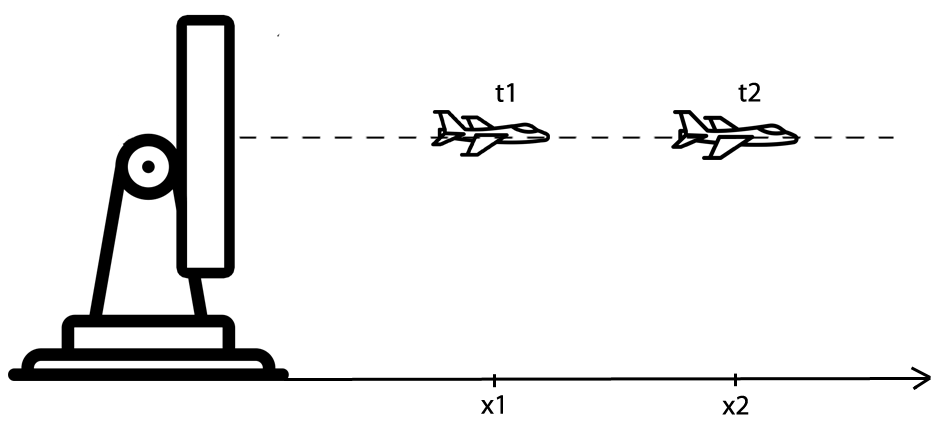
\includegraphics[width=0.9\textwidth]{Figures/Chapter1/ex2_oneD_radar.png}
	    \label{fig:ex2_oneD_radar}
	 \vspace{-10pt}   
	\end{figure}
	\item $x_n$ represents the range to the aircraft at time $n$.
	\item The velocity is a derivative of the range
	$$\dot{x} = v = \frac{dx}{dt}$$
	\end{itemize}
	\column{0.5\textwidth}
	\begin{itemize}
	    \item The radar sends a track beam in the direction of the target at a constant rate, $\Delta t$.
	    \item The system's dynamic model for constant velocity motion is
	    \begin{align*}
	        x_{n+1} & = x_n + \Delta t \dot{x}_n, & [\text{Aircraft range}]\\
	        \dot{x}_{n+1} & = \dot{x}_{n}, & [\text{Constant velocity}]
	    \end{align*}
	    \item This system of eqs. is called as \textcolor{blue}{State Extrapolation Equation} or \textcolor{blue}{Transition Equation} or \textcolor{blue}{Prediction Equation} $\rightarrow$ \textcolor{red}{Also, one of the Kalman Filter equations}.
	\end{itemize}
\end{columns}    
\end{frame}

%-----------------------------------------------------
\begin{frame}{The $\alpha-\beta$ Filter}
\begin{columns}
    \column{0.5\textwidth}
    \begin{itemize}
        \item Assume that at time $n-1$ the estimated range of the aircraft is 30,000m, and its estimated velocity is 40m/s.
        \item Using the system's dynamic model, the target position at time $n$ is (with $\Delta t = 5\,s$)
        \begin{equation}
          \hat{x}_{n, n-1} = \hat{x}_{n-1,n-1} + \Delta t \dot{x}_{n-1,n-1} = 30200m\nonumber  
        \end{equation}
        \item The target velocity prediction for time $n$
        \begin{equation}
          \dot{x}_{n, n-1} = \dot{x}_{n-1,n-1} = 40m/s\nonumber  
        \end{equation}
        \item What if: the radar measures the range $z_n = 30,110$ instead. Two possibilities of the gap:\\
        - The radar measurements are not precise.\\
        - The aircraft velocity has changed. 
        \item Let's update the velocity State Update Equation
        \begin{equation}
          \boxed{\hat{\dot{x}}_{n, n} = \hat{\dot{x}}_{n,n-1} + \beta \left(\frac{z_n - \hat{x}_{n,n-1}}{\Delta t}\right)\nonumber }
        \end{equation}
    \end{itemize}
    \column{0.5\textwidth}
    \begin{itemize}
        \item $\beta$ value depends on the precision level of the radar. If precision level is high, the range difference results from the change in velocity. Therefore, we should set high $\beta$. For $\beta=0.9 \rightarrow \hat{\dot{x}}_{n,n}= 23.8 m/s$
        \item On the other hand, if radar precision is low, the gap results from the radar measurement error. For $\beta=0.1 \rightarrow \hat{\dot{x}}_{n,n}= 38.2 m/s$
        
        \item The range State Update Equation for the aircraft position is (similar to Example~1)
        \begin{equation}
          \boxed{\hat{x}_{n, n} = \hat{x}_{n,n-1} + \alpha \left(z_n - \hat{x}_{n,n-1}\right)\nonumber }
        \end{equation}
        \item $\alpha$-value depends on the radar measurement precision. For high precision radar, we should choose high $\alpha$, giving high weight to the measurements, and lower otherwise.
        
        \item This system of equations, State Update Equations, are also called as \textcolor{blue}{$\alpha-\beta$ track update equations or track filtering equations}. 
        
    \end{itemize}
    
    \end{columns}  
\end{frame}
%-----------------------------------------------------
\begin{frame}{Estimation Algorithm for Example~2}
\begin{columns}
    \column{0.3\textwidth}
    \textbf{Parameters:}\\
    $\alpha=0.2$,\\ $\beta=0.1$,\\ $\Delta t = 5s$
    \column{0.7\textwidth}
        \begin{figure}
	    \centering
	    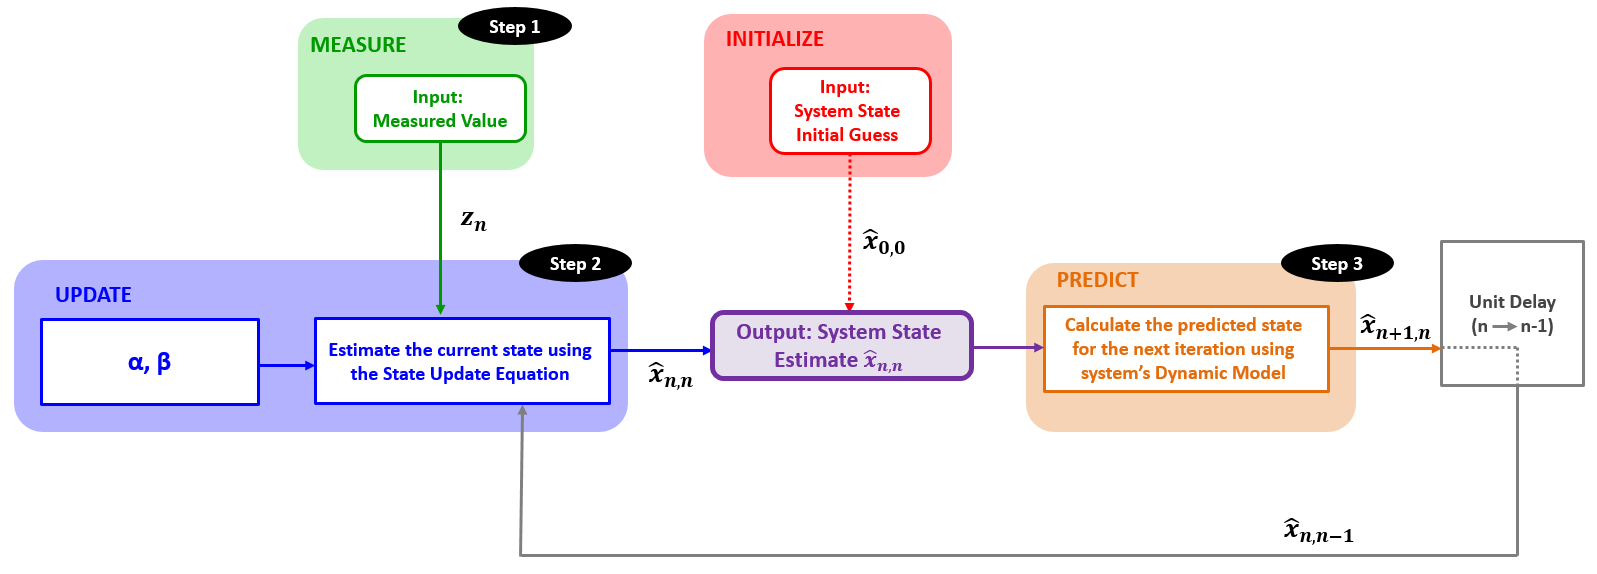
\includegraphics[width=1\textwidth]{Figures/Chapter1/ex2_estimationAlgorithm.png}
	    \label{fig:ex2_estimationAlgorithm}
	    	\vspace{-8pt}
	\end{figure}
\end{columns}
\textbf{Note:} Unlike Example~1, the Gain values $\alpha$ and $\beta$ are given. In the Kalman Filter, the $\alpha$ and $\beta$ are replaced by \textbf{Kalman Gain}, which is calculated at each iteration.\\  
\textbf{Iteration Zero:}
\vspace{5pt}
\begin{columns}
    \column{0.5\textwidth}
    \textbf{Initialization:} Initial Guess:
        $$\hat{x}_{0,0} = 30,000m$$
        $$\hat{\dot{x}}_{0,0} = 40m/s$$
    \textbf{Prediction:} Using the State Extrapolation Eqs., Range prediciton:
    \begin{align*}
        \hat{x}_{n+1,n} & = \hat{x}_{n,n} + \Delta t \hat{\dot{x}}_{n,n}\\
        \hat{x}_{1,0}   & = \hat{x}_{0,0} + \Delta t \hat{\dot{x}}_{0,0} = 30200m
    \end{align*}    
    \column{0.5\textwidth}
    Velocity prediction:
    \begin{align*}
        \hat{\dot{x}}_{n+1,n} & = \hat{\dot{x}}_{n,n}\\
        \hat{\dot{x}}_{1,0}   & = \hat{\dot{x}}_{0,0} = 40m/s
    \end{align*}

\end{columns}



\end{frame}
%-----------------------------------------------------
\begin{frame}{Results for Example~2}
\vspace{-12pt}
\begin{columns}
    \column{0.5\textwidth}
    \begin{figure}
	    \centering
	    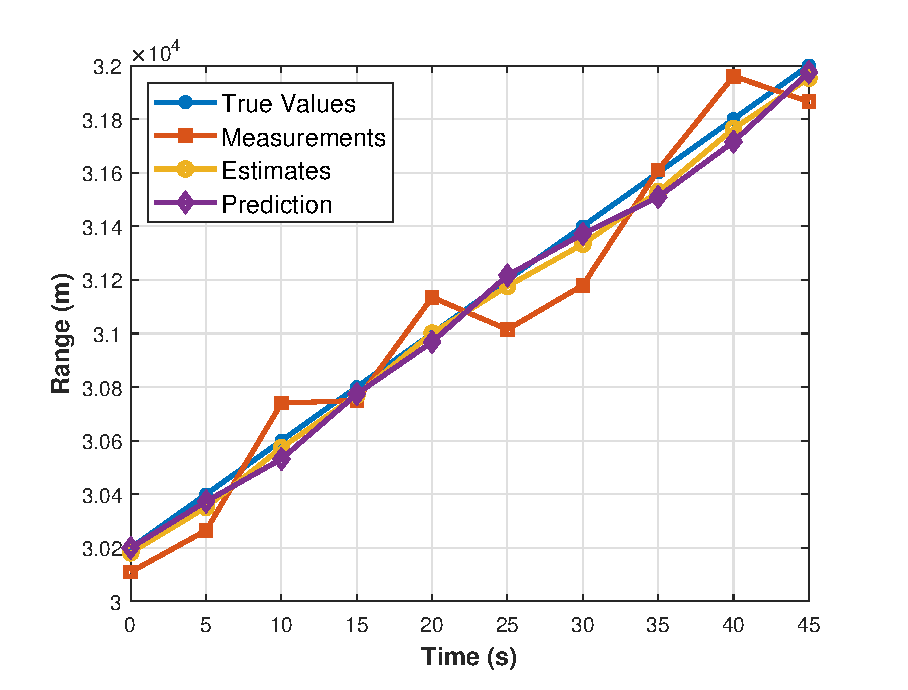
\includegraphics[width=0.9\textwidth]{Figures/Chapter1/ex2_estimationAlgorithm_alpha0.2_beta0.1.eps}
	    \label{fig:ex2_estimationAlgorithm_alpha0.2_beta0.1}
	    \vspace{-15pt}
	    \caption{$\alpha=0.2, \beta=0.1$ }
	    \vspace{-8pt}
	\end{figure}
	The estimation algorithm has a smoothing effect on the measurements and converges toward the true value.
    \column{0.5\textwidth}  
    \begin{figure}
	    \centering
	    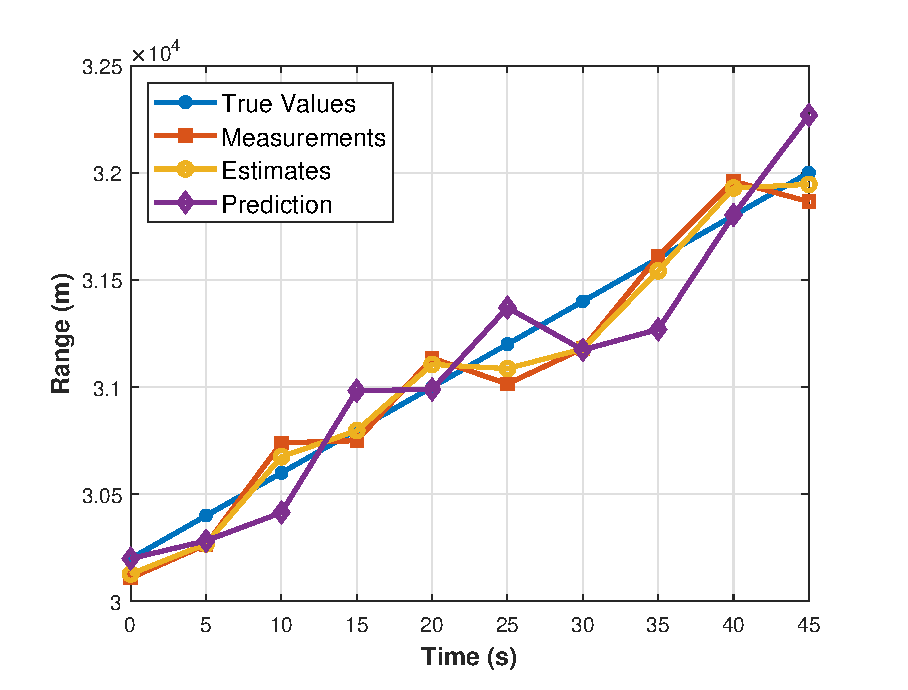
\includegraphics[width=0.9\textwidth]{Figures/Chapter1/ex2_estimationAlgorithm_alpha0.8_beta0.5.eps}
	    \label{fig:ex2_estimationAlgorithm_alpha0.8_beta0.5}
	    \vspace{-15pt}
	    \caption{$\alpha=0.8, \beta=0.5$}
	    \vspace{-8pt}
	\end{figure}
	"Smoothing" degree is much lower. The "current estimate" is very close to the measured values, and predicted estimate errors are high.
\end{columns}
\vspace{7pt}
\textcolor{blue}{$\alpha$ and $\beta$ values should depend on the measurement precision. If we use high precision equipment, we would prefer a high $\alpha$ and $\beta$ that follow measurements. In this case, the filter would quickly respond to a velocity change of the target. OTOH, if measurement precision is low, we prefer low  $\alpha$ and $\beta$. In this case, the filter smoothes the uncertainty (errors) in the measurements. However, the filter reaction to target velocity changes would be much slower.}

\texttt{\tiny [Code: a-b-c Filter/Ex2\_alpha-beta\_EstimationAlgorithm.m]}
\end{frame}
%-----------------------------------------------------
\subsubsection{Example~3: Tracking Accelerating Aircraft in 1D (Another Dynamic System)}
\begin{frame}{Example~3: Tracking Accelerating Aircraft in 1D}
\begin{columns}
    \column{0.5\textwidth}        
    This example tracks an aircraft moving with constant acceleration with the $\alpha-\beta$ filter.
    
    \vspace{5pt}
    
    In Example~2, aircraft was moving at a constant velocity of 40m/s. 
        \begin{figure}
	    \centering
	    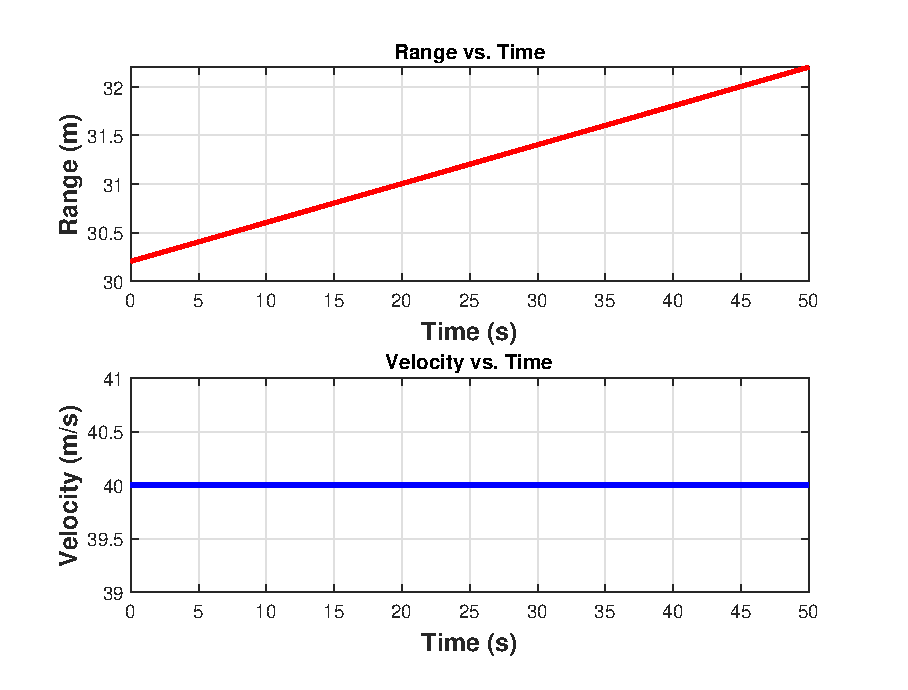
\includegraphics[width=1\textwidth]{Figures/Chapter1/ex3_preliminary1.eps}
	    \label{fig:ex3_preliminary1}
	    \vspace{-8pt}
	\end{figure}
        \texttt{\tiny [Code: a-b-c Filter/Ex3\_preliminary.m]}
    \column{0.5\textwidth} 
    
    Assume, a fighter aircraft moving at a constant velocity of 50\,m/s for 15 seconds. Then the aircraft accelerates with a constant acceleration of $8\,m/s^2$ for another 35 seconds.
        \begin{figure}
	    \centering
	    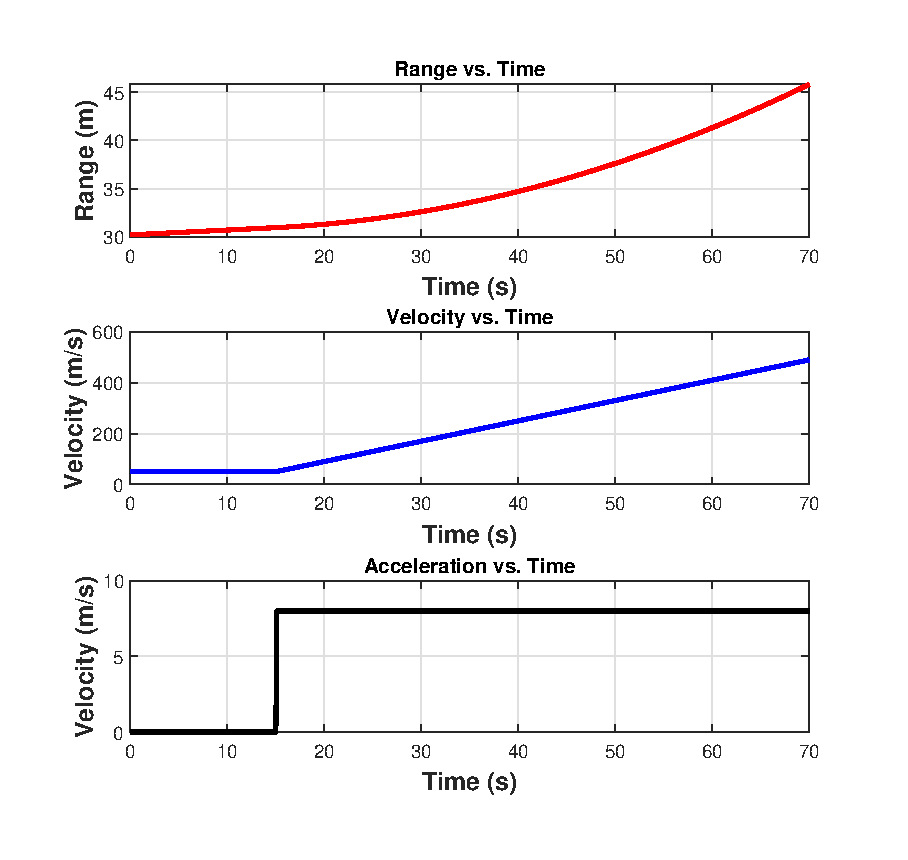
\includegraphics[width=1\textwidth]{Figures/Chapter1/ex3_preliminary2.eps}
	    \label{fig:ex3_preliminary2}
	    \vspace{-20pt}
	\end{figure}
	
Let's track this aircraft with the filter used in Example~2.
\end{columns}    
\end{frame}
%-----------------------------------------------------
\begin{frame}{Example~3: Tracking Accelerating Aircraft in 1D}
\textbf{Parameters:} $\alpha=0.2$, $\beta=0.1$, $\Delta t=5s$\\
\begin{columns}
    \column{0.5\textwidth}
    \begin{figure}
	    \centering
	    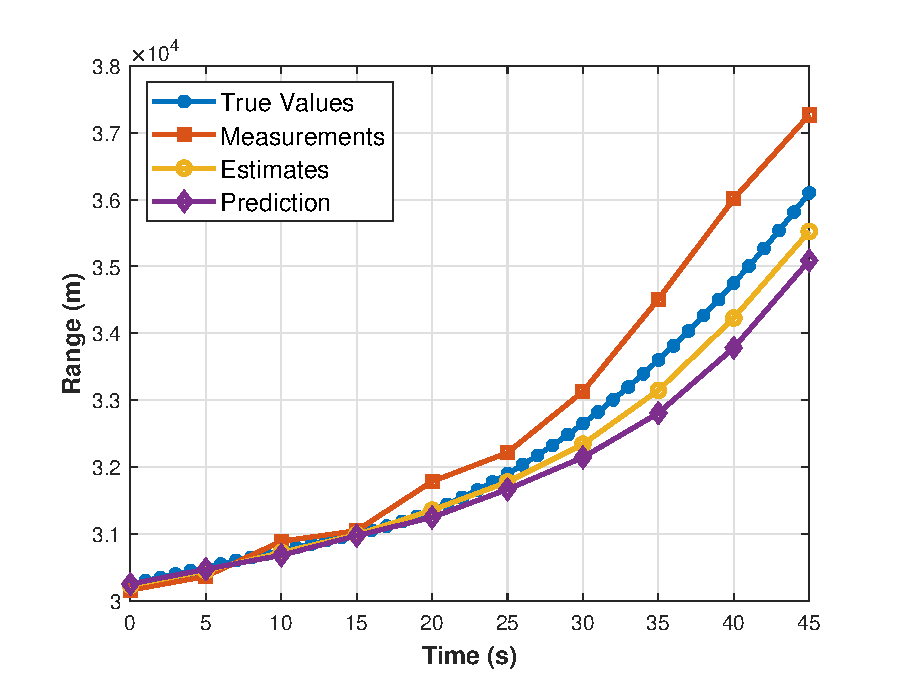
\includegraphics[width=0.9\textwidth]{Figures/Chapter1/ex3_estimationAlgorithm_range.eps}
	    \label{fig:ex3_estimationAlgorithm_range}
	   % \vspace{-20pt}
	\end{figure}
    
    \column{0.5\textwidth}
    \begin{figure}
	    \centering
	    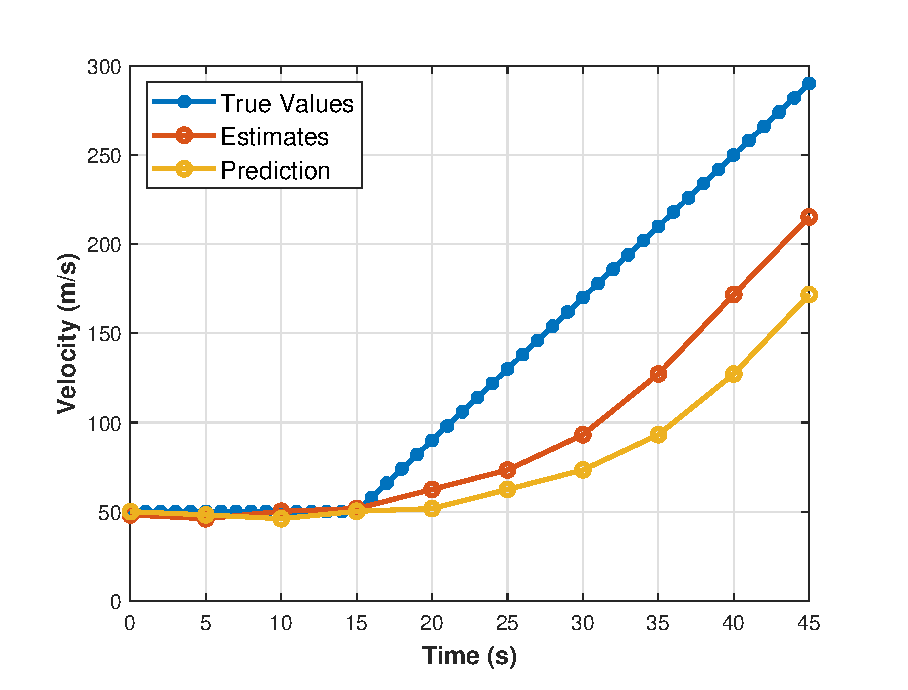
\includegraphics[width=0.9\textwidth]{Figures/Chapter1/ex3_estimationAlgorithm_velocity.eps}
	    \label{fig:ex3_estimationAlgorithm_velocity}
	   % \vspace{-20pt}
	\end{figure}
\end{columns}
There is a constant gap between true or measured values and estimates. The gap is called a \textcolor{blue}{lag error}, or \textcolor{blue}{Dynamic error or Systematic error or Bias error or Truncation error}.
\vspace{5pt}

The lag error appears during the acceleration period. After the acceleration period, the filter closes the gap and converges toward the true value. However, a significant lag error can result in the target loss, which is unacceptable in certain applications, such as missile guidance or air defense.

\texttt{\tiny [Code: a-b-c Filter/Ex3\_alpha-beta\_EstimationAlgorithm.m]}
\end{frame}
%-----------------------------------------------------
\subsubsection{Example 4: Tracking the Accelerating Aircraft with the $\alpha-\beta-\gamma$ Filter}
\begin{frame}{Example 4: Tracking the Accelerating Aircraft with the $\alpha-\beta-\gamma$ Filter}
\begin{columns}
    \column{0.5\textwidth}
    \vspace{-20pt}
    \begin{center}
    \begin{minipage}{1\linewidth} % Adjust the minipage width as needed
    \begin{exampleblock}{\textbf{State Extrapolation Equations:}}
        \begin{align*}
            \hat{x}_{n+1,n} & = \hat{x}_{n,n} + \hat{\dot{x}}_{n,n}\Delta_t + \hat{\ddot{x}}_{n,n}\frac{\Delta_t^2}{2}\\
            \hat{\dot{x}}_{n+1,n} & = \hat{\dot{x}}_{n,n} + \hat{\ddot{x}}_{n,n}\Delta_t\\
            \hat{\ddot{x}}_{n+1,n} & = \hat{\ddot{x}}_{n,n}
        \end{align*}
    \end{exampleblock}
    \end{minipage}
\end{center}
    
    \column{0.5\textwidth}
    \vspace{-20pt}
    \begin{center}
    \begin{minipage}{1\linewidth} % Adjust the minipage width as needed
    \begin{exampleblock}{\textbf{State Update Equations:}}
    \begin{align*}
        \hat{x}_{n,n} & = \hat{x}_{n,n-1} + \alpha (z_n - \hat{x}_{n,n-1})\\
        \hat{\dot{x}}_{n,n} & = \hat{\dot{x}}_{n,n-1} + \beta\left(\frac{z_n - \hat{x}_{n,n-1}}{\Delta_t}\right)\\
        \hat{\ddot{x}}_{n,n} & = \hat{\ddot{x}}_{n,n-1} + \gamma\left(\frac{z_n - \hat{x}_{n,n-1}}{0.5\Delta_t^2}\right)
    \end{align*}
        \end{exampleblock}
    \end{minipage}
\end{center}
\end{columns}
\noindent\rule{5cm}{0.4pt}

    \textbf{Scenario from Example 3:} an aircraft that moves with a constant velocity of 50m/s for 15 seconds and then accelerates with a constant acceleration of $8m/s^2$ for another 35 seconds.
    
\noindent\rule{5cm}{0.4pt}

\begin{columns}    
    \column{0.5\textwidth}
    
    \vspace{4pt}
    \textbf{The $\alpha-\beta-\gamma$ filter parameters:}
    \begin{itemize}
        \item $\alpha=0.5$
        \item $\beta=0.4$
        \item $\gamma=0.1$
        \item $\Delta_t = 5s$
    \end{itemize}
    \column{0.5\textwidth}
    \textbf{Initialization:}
    \begin{itemize}
        \item $\hat{x}_{0,0} = 30,000$\,m
        \item $\hat{\dot{x}}_{0,0} = 50$\,m/s
        \item $\hat{\ddot{x}}_{0,0} = 0$\,m/$\text{s}^2$
    \end{itemize}    
\end{columns}    
\end{frame}

%-----------------------------------------------------
\begin{frame}{Example 4: Results}
\begin{columns}
    \column{0.6\textwidth}
    \begin{figure}
	    \centering
	    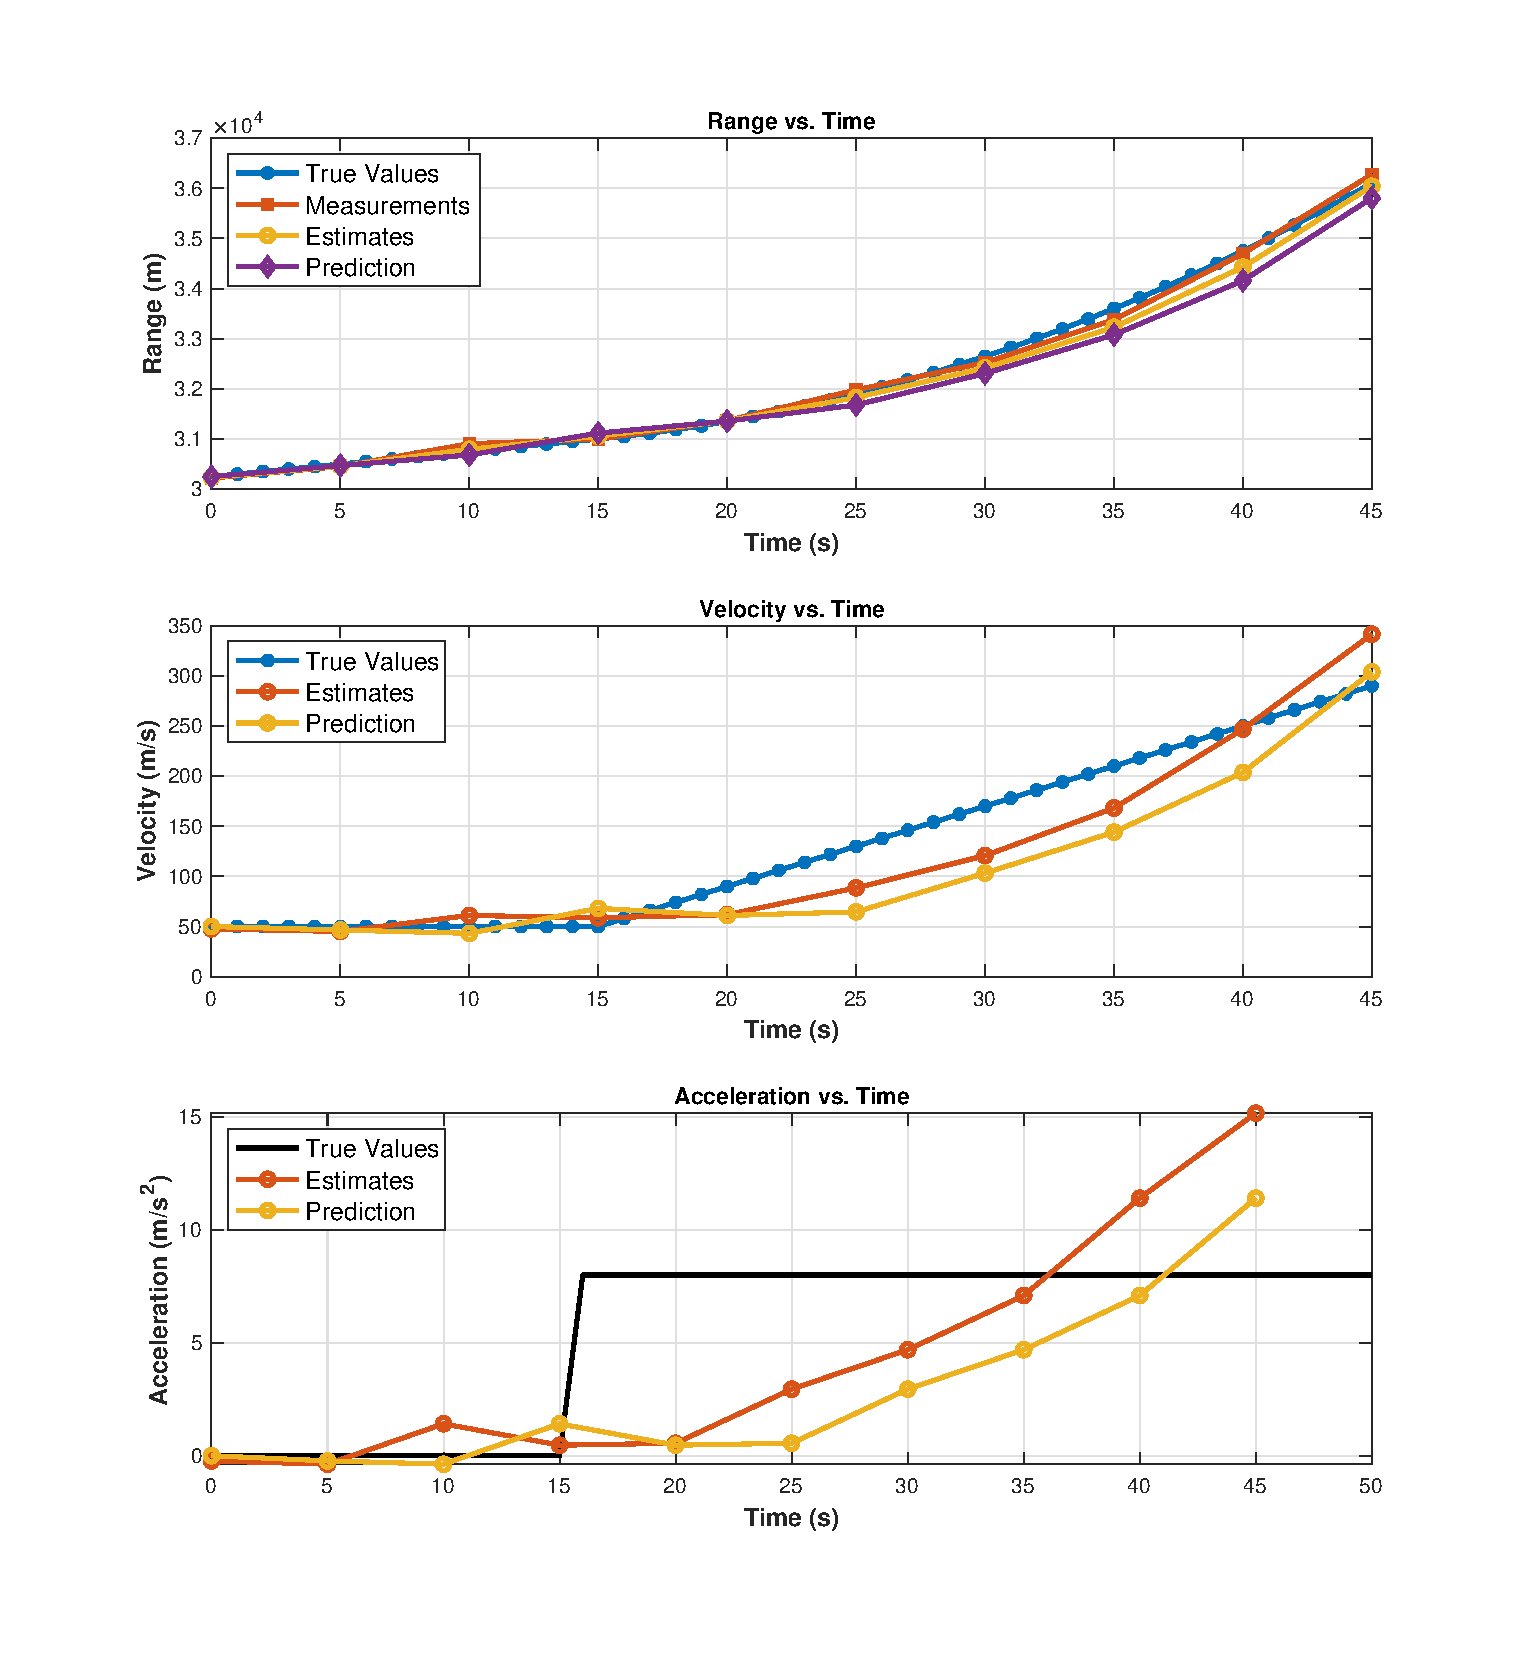
\includegraphics[width=0.9\textwidth]{Figures/Chapter1/ex4_estimationAlgorithm.eps}
	    \label{fig:ex4_estimationAlgorithm}
	   % \vspace{-20pt}
	\end{figure}
	\texttt{\tiny [Code: a-b-c Filter/Ex4\_alpha-beta-gamma\_EstimationAlgorithm.m]}
    \column{0.4\textwidth}
    \begin{itemize}
        \item The $\alpha-\beta-\gamma$ filter with dynamic model equations that include acceleration can track the target with constant acceleration and eliminate the lag error.
        \item But what happens in the case of a maneuvering target? The target can suddenly change the flight direction by making a maneuver. The target's dynamic model can also include a jerk (changing acceleration). 
        \item In such cases, the $\alpha-\beta-\gamma$  filter with constant $\alpha-\beta-\gamma$ coefficients produces estimation errors and, in some cases, loses the target track.
        \item \textcolor{blue}{The Kalman filter can handle uncertainty in the dynamic model.}
    \end{itemize}
\end{columns}    
\end{frame}
%-----------------------------------------------------
\begin{frame}{Summary of the $\alpha-\beta-\gamma$ Filter}

\begin{itemize}
    \item There are many types of $\alpha-\beta-\gamma$  filters, based on the same principle:
    \begin{itemize}
        \item The current state estimation is based on the state update equations.
        \item The following state estimation (prediction) is based on the dynamic model equations.
    \end{itemize}
    \item The main difference between these filters is the selection of weighting coefficients. \textcolor{blue}{Some filter types use constant, others compute at every iteration}
    \item Selection of parameters is discussed in detail in
        \begin{itemize}
            \item Dirk Tenne, Tarunraj Singh. "Optimal Design of $\alpha-\beta-\gamma$ Filters". State University of New York at Buffalo.
        \end{itemize}
    \item Another important issue is the initiation of the filter, i.e., providing the initial value for the first filter iteration.
\end{itemize}
    
\end{frame}

%-----------------------------------------------------
\begin{frame}{Most Popular $\alpha-\beta-\gamma$ Filters}
\begin{itemize}
    \item Wiener Filter
    \item Bayes Filter
    \item Fading-memory polynomial Filter
    \item Expanding-memory (or growing-memory) polynomial Filter
    \item Least-squares Filter
    \item Benedict–Bordner Filter
    \item Lumped Filter
    \item Discounted least-squares $\alpha-\beta$ Filter
    \item Critically damped $\alpha-\beta$ Filter
    \item Growing-memory Filter
    \item Kalman Filter
    \item Extended Kalman Filter
    \item Unscented Kalman Filter
    \item Extended Complex Kalman Filter
    \item Gauss-Hermite Kalman Filter
    \item Cubature Kalman Filter
    \item Particle Filter
\end{itemize}

    
\end{frame}

%-----------------------------------------------------
\subsection{One-Dimensional Kalman Filter without Process Noise}
\begin{frame}{One Dimensional Kalman Filter without Process Noise}
\begin{columns}

    \column{0.53\textwidth}
\textbf{Example~1: Gold Bar Weight Measurements.}\\
\textbf{Measurement errors:}
\begin{itemize}
    \item The different between true values and measurements; often described by variance ($\sigma^2$) for their randomness.
    \item The variance of the measurement errors could be provided by the scale vendor or \textcolor{blue}{derived by a calibration procedure}.
    \item The variance of the measurement errors is the \textcolor{blue}{measurement uncertainty}, denoted by $r$.
\end{itemize}
\textbf{Estimate error}
\begin{itemize}
    \item The difference between the estimates and the true values is the estimate error. 
    \item the estimate error becomes smaller and smaller as we make additional measurements, and it converges towards zero, while the estimated value converges towards the true value. 
    \item We don't know the estimate error, but we can estimate the uncertainty in estimate, denoted by $p$ (\textcolor{blue}{estimate variance}).
\end{itemize}
	\column{0.47\textwidth}
	            \begin{figure}
		    \centering
		   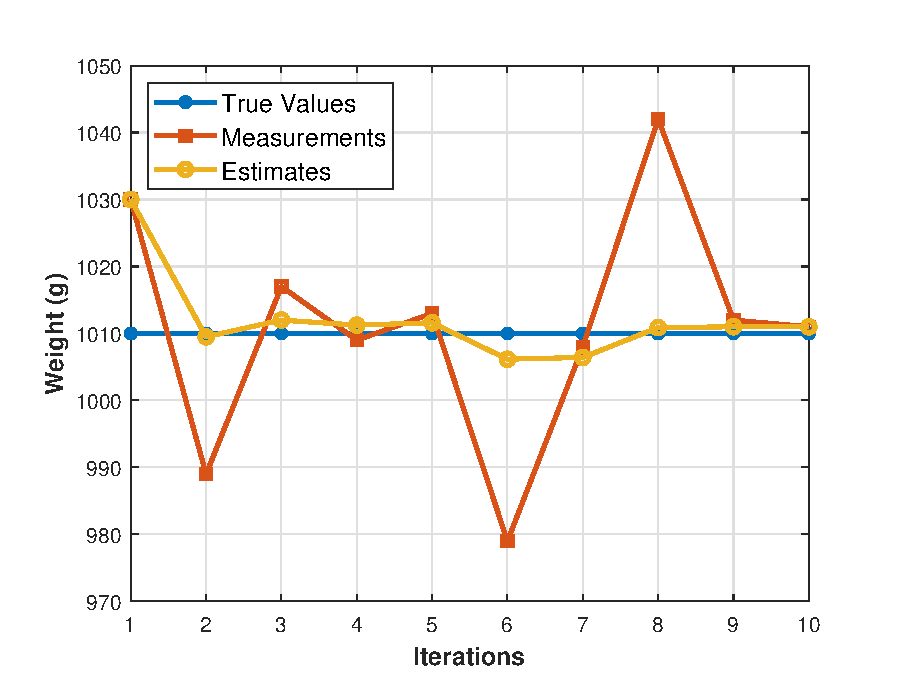
\includegraphics[width=1\textwidth]{Figures/Chapter1/ex1_estimationAlgorithm.eps}
		    \label{fig:ex1_estimationAlgorithm}
	    \end{figure}
	    \vspace{-12pt}
        \begin{figure}
		    \centering
		   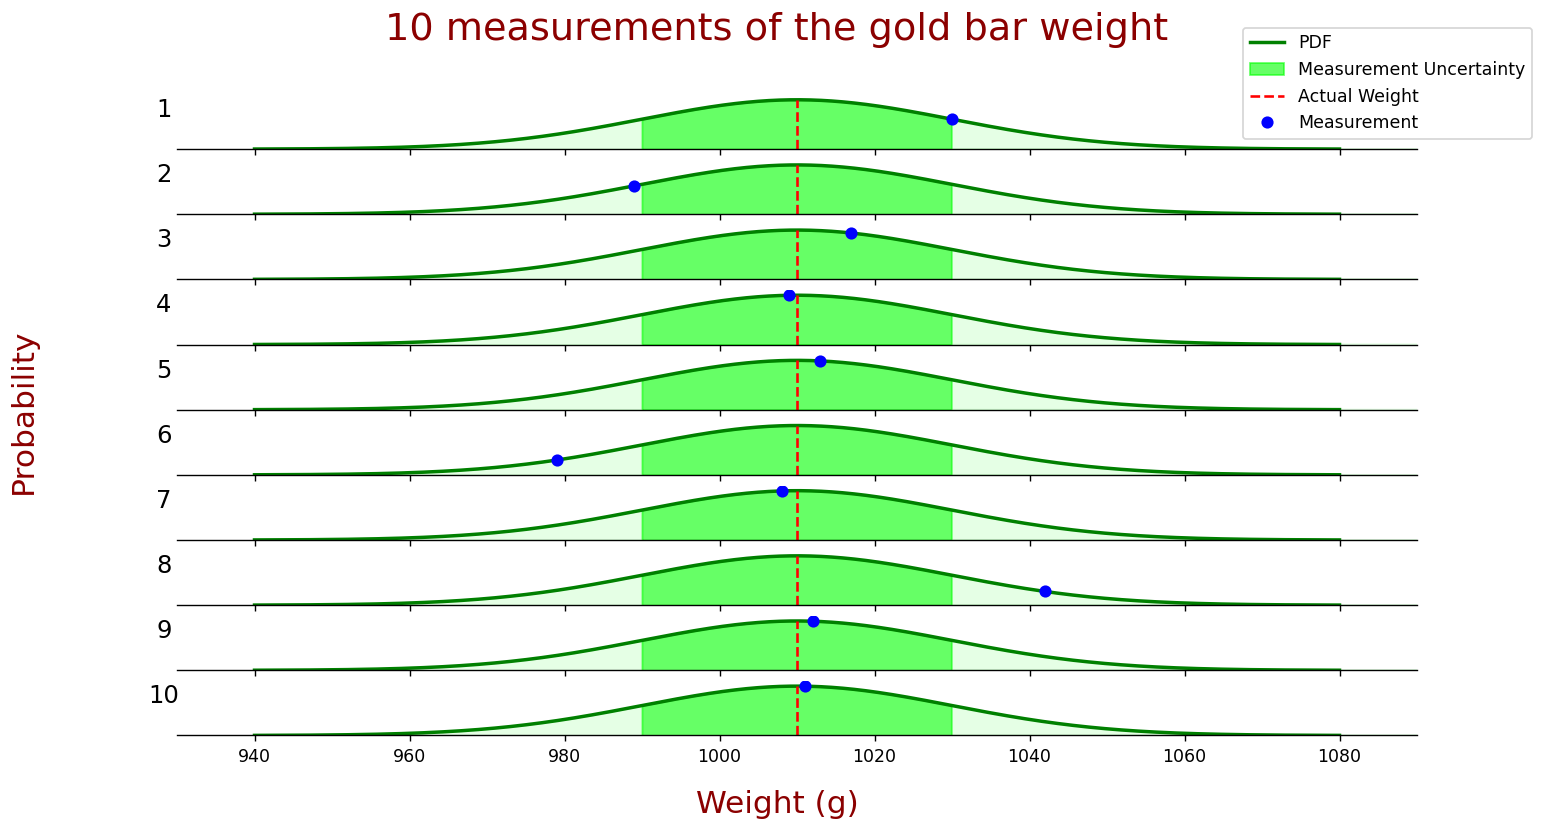
\includegraphics[width=1\textwidth]{Figures/Chapter1/PDFs.png}
		    \label{fig:PDFs}
	    \end{figure}
\end{columns}
    
\end{frame}

%-----------------------------------------------------
\begin{frame}{State Prediction: Estimate Uncertainty Extrapolation or Covariance Extrapolation Equation (Eq.~3)}
Like state extrapolation, the estimate uncertainty extrapolation is done with the dynamic model equations.
\begin{columns}
    \column{0.5\textwidth}
        \begin{itemize}
            \item In Example~1 (gold bar weight measurement), the system's dynamics is constant. Thus, the estimate uncertainty extrapolation is:
            $$p_{n+1,n} = p_{n,n}$$
            where $p$ is the gold bar's weight estimate uncertainty
            
            \item In Example~2, the predicted target position is:
            \begin{align*}
	            \hat{x}_{n+1,n} & = \hat{x}_{n,n} + \Delta t \hat{\dot{x}}_{n,n}, & [\text{Aircraft range}]\\
	        \hat{\dot{x}}_{n+1,n} & = \hat{\dot{x}}_{n,n}, & [\text{Constant velocity}]
	    \end{align*}
	    i.e., the predicted position equals the current estimated position + the current estimated velocity x time. The predicted velocity equals the current velocity estimate (assuming a constant velocity model).
    
\end{itemize}
    \column{0.5\textwidth}
    \begin{itemize}
        \item The estimate uncertainty extrapolation would be:
        \begin{empheq}[box=\mymath]{gather*}
	            p_{n+1,n}^x = p_{n,n}^x + \Delta t^2 p_{n,n}^v,\\
	        p_{n+1,n}^v = p_{n,n}^v
	    \end{empheq}
	    where\\
	    $p^x$ is the position estimate uncertainty
	    $p^v$ is the velocity estimate uncertainty
    
        i.e., the predicted position estimate uncertainty equals the current position estimate uncertainty + current velocity estimate uncertainty $\times$ by time squared. The predicted velocity estimate uncertainty equals the current velocity estimate uncertainty (assuming a constant velocity model).
    \end{itemize}
    
\end{columns}


\end{frame}
%-----------------------------------------------------
\begin{frame}{State Prediction Illustration}
            \begin{figure}
		    \centering
		   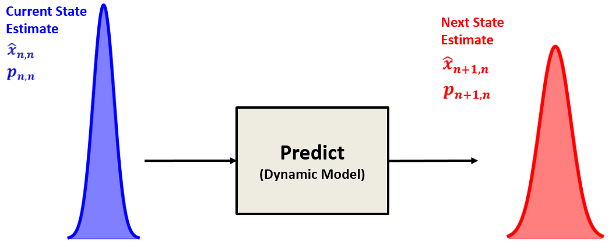
\includegraphics[width=0.7\textwidth]{Figures/Chapter1/StatePredictionIllustration.png}
		    \label{fig:SatePrediction}
	    \end{figure}

    Note that for any normally distributed random variable $x$ with variance $\sigma^2$, $kx$ is distributed normally with variance $k^2\sigma^2$, therefore the time term in the uncertainty extrapolation equation is squared. 
\end{frame}
%-----------------------------------------------------
\begin{frame}{State Update: Kalman Gain Equation (Eq.4)}

To estimate the current state of the system, we combine two RVs:
    \begin{itemize}
        \item The prior state estimate (the current state estimate predicted at the previous state).
        \item The measurement
    \end{itemize}
    \begin{figure}
	 \centering
	 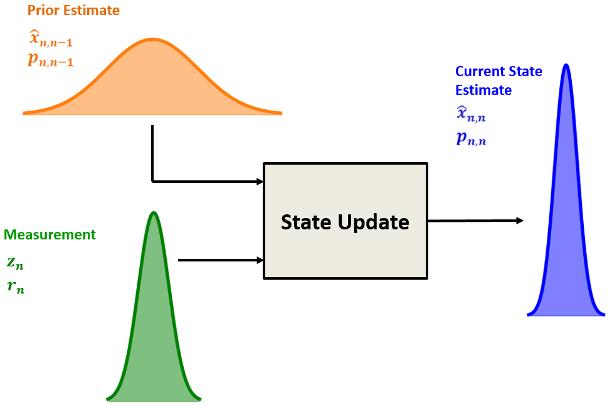
\includegraphics[width=0.5\textwidth]{Figures/Chapter1/StateUpdateIllustration.png}
	 \label{fig:SateUpdate}
    \end{figure}
\end{frame}

%-----------------------------------------------------
\begin{frame}{Kalman Gain cont...}
\textbf{The Kalman Filter is the optimal filter; it combines the prior state estimate with the measurements such that it minimizes the current state estimate uncertainty.} Derivation for 1D Kalman Filter:
\begin{columns}
    \column{0.5\textwidth}
        \begin{itemize}
            \item Given the measurement $z_n$ and the prior estimate $\hat{x}_{n,n-1}$, we want to find an optimum combined estimate $\hat{x}_{n,n}$ based on the measurement and the prior estimate.
            \item Which is actually a weighted mean of the prior estimate and the measurement:
            $$\hat{x}_{n,n}=k_1 z_n + k_2 \hat{x}_{n,n-1}$$
            Where $k_1$ and $k_2$ are the weights of the measurement and the prior estimate, i.e.,
            $$k_1 + k_2 = 1$$
            $$\hat{x}_{n,n}=k_1 z_n + (1-k_1) \hat{x}_{n,n-1}$$
            \item Since, for any normally distributed random variable $x$ with variance $\sigma^2$, $kx$ is distributed normally with variance $k\sigma^2$, thus:
            $${p}_{n,n}=k_1^2 r_n + (1-k_1)^2 {p}_{n,n-1}$$
    \end{itemize}
    \column{0.5\textwidth}
    where:\\
    $p_{n,n}$ is the variance of the optimum combined estimate $\hat{x}_{n,n}$\\
    $p_{n,n-1}$ is the variance of the prior estimate $\hat{x}_{n,n-1}$\\
    $r_n$ is the variance of the measurement $z_n$
    \begin{itemize}
        \item Since we are looking for an \textbf{optimum} estimate, we are interested to minimize $p_{n,n}$.
        \item To find $k_1$ that minimizes $p_{n,n}$, we differentiate $p_{n,n}$ with respect to $k_1$ and set the result to zero, i.e.,
        $$\frac{d p_{n,n}}{d k_1} = 2k_1r_n - 2 (1-k_1)p_{n,n-1}$$
        
        \boxed{
        $$\implies k_1 = \frac{p_{n,n-1}}{p_{n,n-1} + r_n}$$
        }
        \item Since the Kalman Gain yields the minimum variance estimate, the Kalman Filter is also called an \textbf{optimal filter}.
    \end{itemize}
\end{columns}
%-----------------------------------------------------

\end{frame}
\begin{frame}{State Update: Kalman Gain Equation (Eq.4)}

The Kalman Gain (denoted by $Kn$) is the weight given to the current state estimate and the measurements:

\begin{equation*}
    \boxed{K_n = \frac{\text{Uncertainty in Estimate}}{\text{Uncertainty in Estimate} + \text{Uncertainty in Measurement}} = \frac{p_{n,n-1}}{p_{n,n-1} + r_n}}
\end{equation*}
where $p_{n,n-1}$ is the extrapolated estimate uncertainty.
\begin{itemize}
    \item The Kalman Gain is a number between zero and one: $0\leq K_n \leq 1$
    \item Rewrite state update equation:
    $$\hat{x}_{n,n} = \hat{x}_{n,n-1} + K_n\left(z_n-\hat{x}_{n,n-1}\right) = \underbrace{(1-K_n)}_{\text{Current State Estimate Weight}}\hat{x}_{n,n-1} + \underbrace{K_n}_{\text{Measurement Weight}} z_n$$
    % \item The Kalman Gain ($K_n$) is the measurement weight, and the ($1-K_n$) term is the weight of the current state estimate.
    
    \item When the measurement uncertainty is large and the estimate uncertainty is low, the Kalman Gain is close to zero. Hence we give significant weight to the estimate and a small weight to the measurement.

\item OTOH, when the measurement uncertainty is low and the estimate uncertainty is large, the Kalman Gain is close to one. Hence we give a low weight to the estimate and a significant weight to the measurement.

\item If the measurement uncertainty equals the estimate uncertainty, then the Kalman gain equals 0.5.
\end{itemize}
\begin{exampleblock}{}
  {\large ``The Kalman gain tells how much the measurement changes the estimate.''}
\end{exampleblock}
\end{frame}

%-----------------------------------------------------
\begin{frame}{Estimate Uncertainty Update or Covariance Update Equation (Eq.~5)}
% \begin{columns}
    % \column{0.5\textwidth}        
    \textcolor{blue}{Estimate uncertainty update}, also called as \textcolor{blue}{Covariance Update Equation} is defined as
    \begin{empheq}[box=\mymath]{gather*}
        p_{n,n} = (1-K_n)p_{n,n-1},
    \end{empheq}
    where\\
    $K_n$~~~~~~is the Kalman Gain\\
    $p_{n,n-1}$ is the estimate uncertainty, calculated\\~~~~~~~~~during previous filter estimation\\
    $p_{n,n}$~~~~is estimate uncertainty of current state
    
    \vspace{5pt}
    \begin{itemize}
        \item Since $(1-K_n)\leq 1$, the estimate uncertainty is constantly getting smaller with each filter iteration. 
        
        \item When the measurement uncertainty is large, the Kalman gain is low. Therefore, the convergence of the estimate uncertainty would be slow. 
        
        \item However, the Kalman gain is high when the measurement uncertainty is small. Therefore, the estimate uncertainty would quickly converge towards zero.
    \end{itemize}
    
    % \column{0.5\textwidth}

% \end{columns}    
\end{frame}


\begin{frame}{Let's Put it All Together - Basic}
Like the $\alpha - \beta (-\gamma)$ filter, the Kalman filter utilizes the "Measure, Update, Predict" algorithm.
% \begin{columns}
    % \column{0.52\textwidth}
        \begin{figure}
		   \centering
		   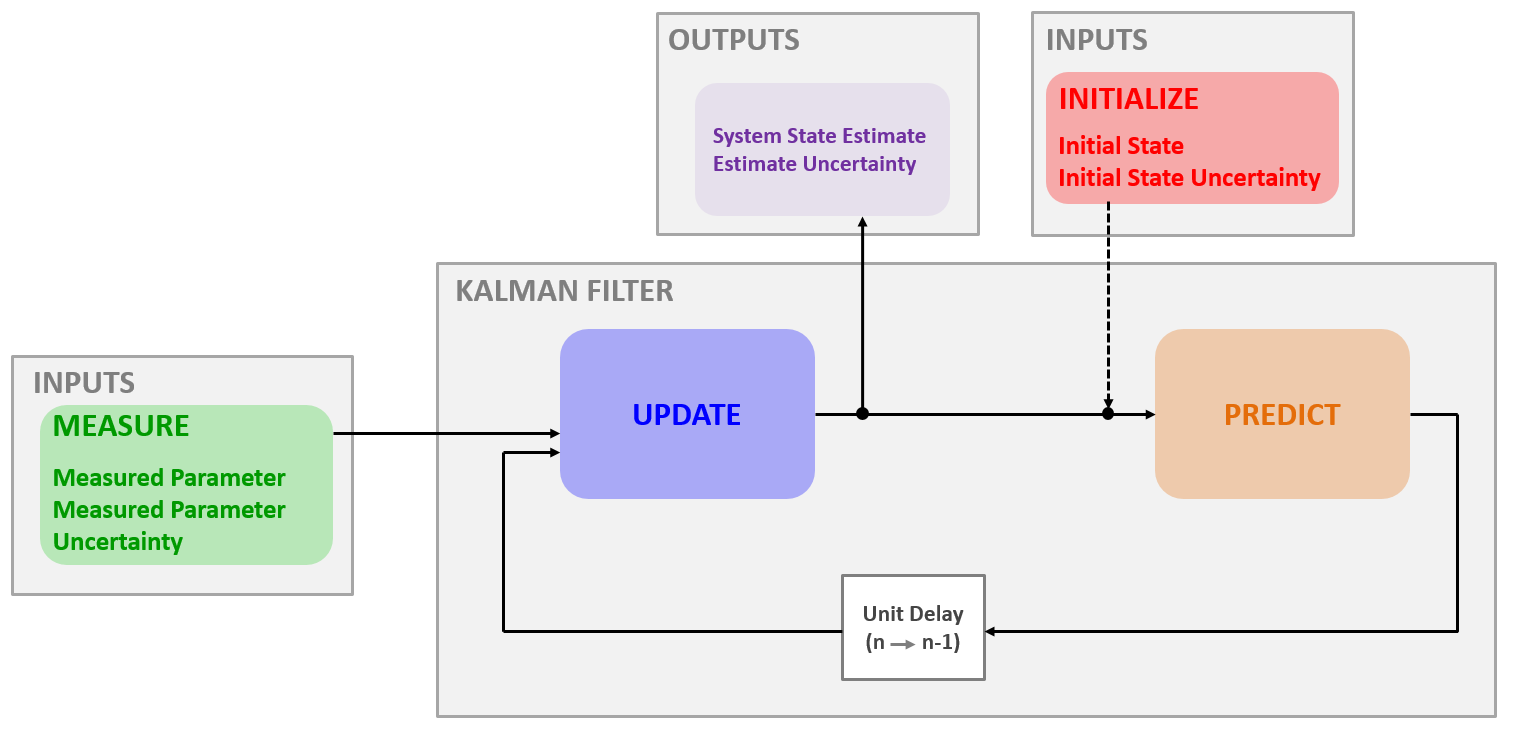
\includegraphics[width=0.6\textwidth]{Figures/Chapter1/KalmanFilterAlgorithm.png}
		   \label{fig:PDFs}
	    \end{figure}
	    \vspace{-10pt}
	\textbf{Inputs:}
	\begin{itemize}
	    \item Initialization: (performed only once). Init. parameters can be provided by another system or process or an educated guess based on experience/theoretical knowledge. If not precise, Kalman filter tries to converge toward true value.
	       \begin{itemize}
	           \item Initial System State $(\hat{x}_{0,0})$
	           \item Initial Uncertainty $(p_{0,0})$
	       \end{itemize} 
	    \item Measurement:(performed at each filter cycle)
	        \begin{itemize}
	           \item Measured System State $(z_n)$
	           \item Measurement Uncertainty $(r_n)$. Usually,  $r_n$ is provided by the equipment vendor, or can be derived from equipment calibration. For example, the radar measurement uncertainty depends on several parameters such as SNR, beam width, bandwidth, time on target, clock stability, and more. While, every radar measurement has a different SNR, beam width, and time on target.
	       \end{itemize} 
	\end{itemize}
\end{frame}
%-----------------------------------------------------
\begin{frame}{Let's Put it All Together - Basic (Cont.)}
Contrary to the $\alpha - \beta (- \gamma)$ filter, the Kalman Filter treats measurements, current state estimation, and next state estimation (predictions) as normally distributed random variables.
% \begin{columns}
    % \column{0.52\textwidth}
        \begin{figure}
		   \centering
		   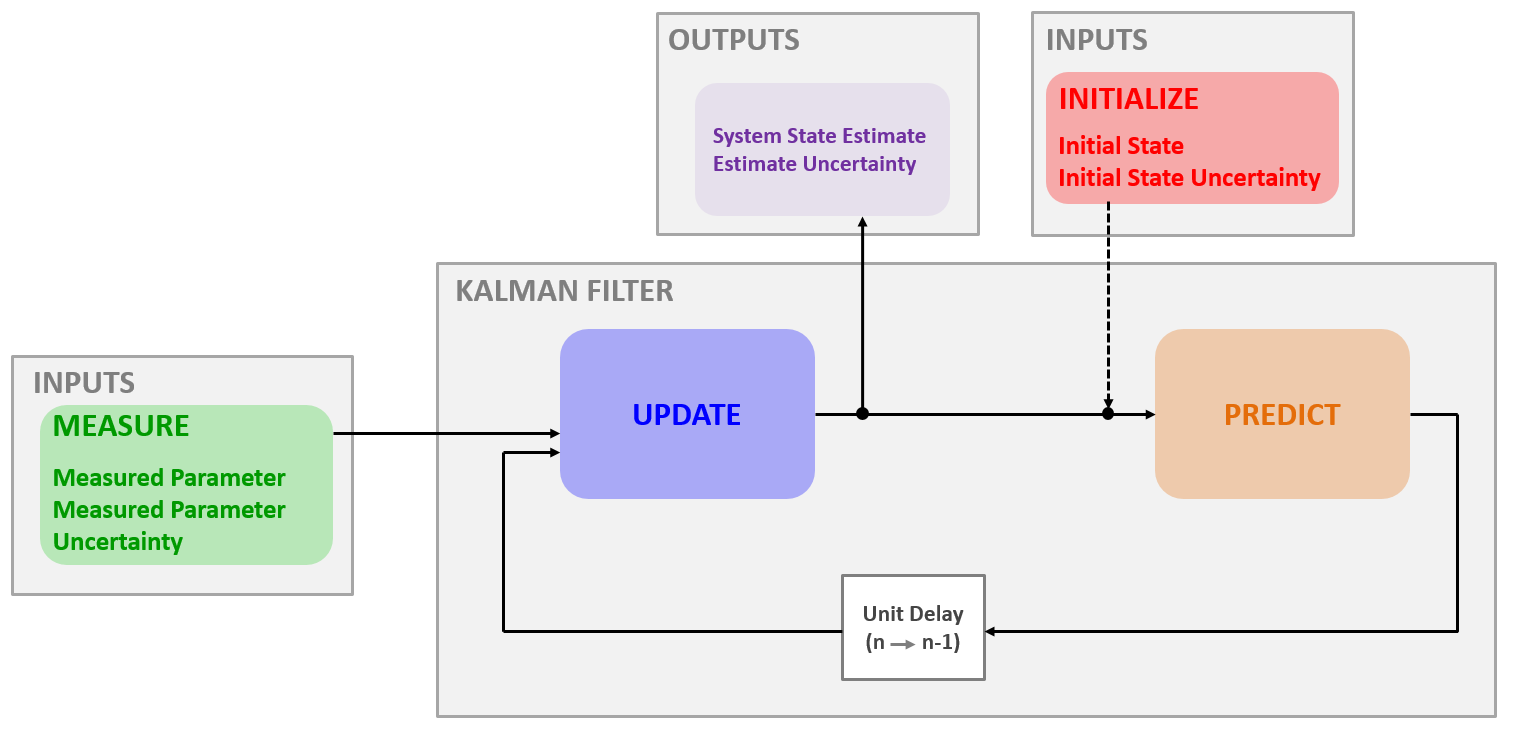
\includegraphics[width=0.6\textwidth]{Figures/Chapter1/KalmanFilterAlgorithm.png}
		   \label{fig:PDFs}
	    \end{figure}
	   % \vspace{-10pt}
	\textbf{Outputs:}
	\begin{itemize}
       \item System State Estimate $(\hat{x}_{n,n})$
       \item Estimate Uncertainty $(p_{n,n})$. 
       
       Since $p_{n,n} = (1-K_n)p_{n,n-1}$, $p_{n,n}$ is getting smaller with each filter iteration, as $(1-K_n)\leq1$. So it's up to us to decide how many measurements to take.
	\end{itemize}
\end{frame}


%-----------------------------------------------------
\begin{frame}{Let's Put it All Together - Basic (Cont.)}

% \begin{table}[]
%     \centering
%     \begin{tabular}{lll}
%         \toprule
%         \textbf{Equation} & \textbf{Equation Name} & \textbf{Alternative names} \\
%         \toprule
%         $\hat{x}_{n,n}= \hat{x}_{n,n-1} + K_n(z_n-\hat{x}_{n,n-1})$ & State Update & Filtering Equation \\ \hline
%         \begin{tabular}[c]{@{}l@{}} $\hat{x}_{n+1,n}= \hat{x}_{n,n} + \Delta t \hat{\dot{x}}_{n,n}$ \\ $\hat{\dot{x}}_{n+1,n} = \hat{\dot{x}}_{n,n}$ \\ (for constant velocity dynamics) \end{tabular} & State Extrapolation & \begin{tabular}[c]{@{}l@{}}Predictor Equation\\ Transition Equation\\ Prediction Equation \\ Dynamic Model \\ State Space Model \end{tabular} \\ \hline
%         $K_n = \dfrac{p_{n,n-1}}{p_{n,n-1} + r_n}$ & Kalman Gain & Weight Equation \\ \hline
%         $p_{n,n} = (1-K_n)p_{n,n-1}$ & Covariance Update & Corrector Equation \\ \hline
%         \begin{tabular}[c]{@{}l@{}} $p_{n+1,n} = p_{n,n}$ \\ (For constant dynamics) \end{tabular} & Covariance Extrapolation & Predictor Covariance Eq.\\
%         \bottomrule
%     \end{tabular}

    \begin{figure}
	   \centering
	   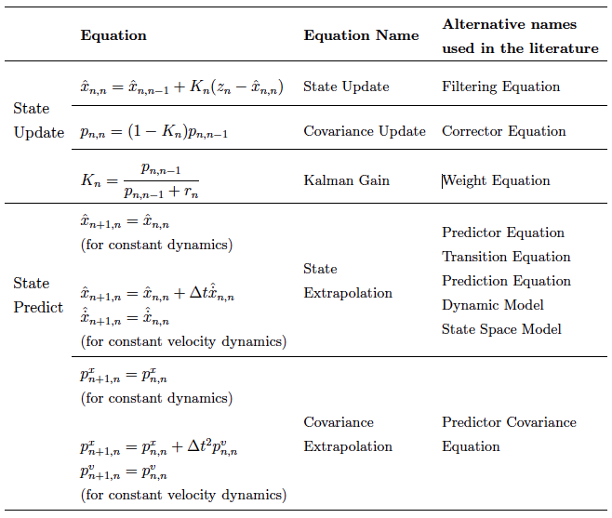
\includegraphics[width=0.75\textwidth]{Figures/Chapter1/KalmanFilterSummery.png}
	       \caption{Summary of Kalman Filter equations for a specific case (i.e., Example~2) }
    \label{tab:my_label}
	   \vspace{-10pt}
	   \end{figure}


%\end{table}
% }



\end{frame}
%-----------------------------------------------------

\begin{frame}{Let's Put it All Together - Detailed}

\begin{columns}
    \column{0.5\textwidth}
        \begin{figure}
	   \centering
	   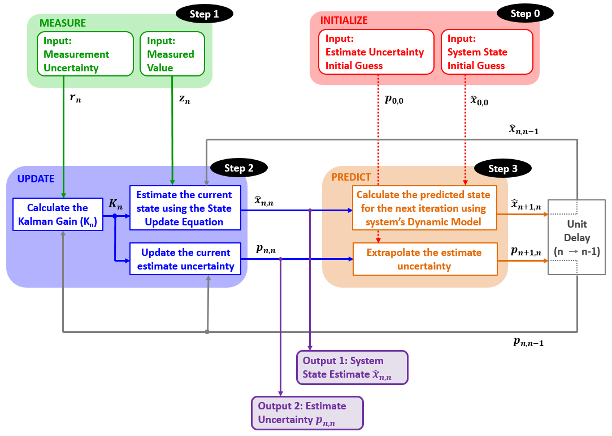
\includegraphics[width=1\textwidth]{Figures/Chapter1/DetailedKalmanFilterAlgorithm.png}
	   \label{fig:DetailedKalmanFilterAlgorithm}
	   \vspace{-10pt}
	   \end{figure}

	\begin{itemize}
	    \item \textbf{Step 0: Initialization}
	       \begin{itemize}
	           \item Initial System State $(\hat{x}_{0,0})$
	           \item Initial Uncertainty $(p_{0,0})$
	       \end{itemize} 
	    \item \textbf{Step 1: Measurement}
	        \begin{itemize}
	           \item Measured System State $(z_n)$
	           \item Measurement Uncertainty $(r_n)$. 
	       \end{itemize} 
	\end{itemize}
		
	\column{0.5\textwidth} 
            \begin{itemize}
            \item \textbf{Step 2 - Inputs:} State Update (estimation of the system's current state). 
	        \begin{itemize}
	           \item Measured value $(z_n)$
	           \item Measurement Uncertainty $(r_n)$. 
	           \item Previous System State Estimate $(\hat{x}_{n,n-1})$
	           \item Estimate Uncertainty $(p_{n,n-1})$
	       \end{itemize} 
        \end{itemize}
	       Based on the inputs, the state update process calculates the Kalman Gain and provides two outputs:

	        \begin{itemize}
	            \item Current System State Estimate $(\hat{x}_{n,n})$
	            \item Current State Estimate Uncertainty $(p_{n,n})$
	        \end{itemize}
	    \begin{itemize} 
	        \item \textbf{Step 3: Prediction:}
	        \begin{itemize}
	            \item The prediction process extrapolates the current system state and uncertainty of the current system state estimate to the next system state, based on the system's dynamic model.
	            \item At the first filter iteration the initialization outputs are treated as the Previous State Estimate and Uncertainty.
	            \item The prediction outputs become the Previous State Estimate and Uncertainty on the following filter iterations.
	        \end{itemize}
	        
	            
	    \end{itemize}
\end{columns}	   	
\end{frame}

%-----------------------------------------------------

\begin{frame}{Kalman Gain Intuition - High Kalman Gain}
The Kalman Gain defines the weight of the measurement ($z_n$) and the weight of the previous estimate ($\hat{x}_{n,n-1}$) when forming a new estimate ($\hat{x}_{n,n}$).

\vspace{5pt}
A low measurement uncertainty relative to the estimate uncertainty would result in a high Kalman Gain (close to 1). Therefore the new estimate would be close to the measurement.
    \begin{figure}
	   \centering 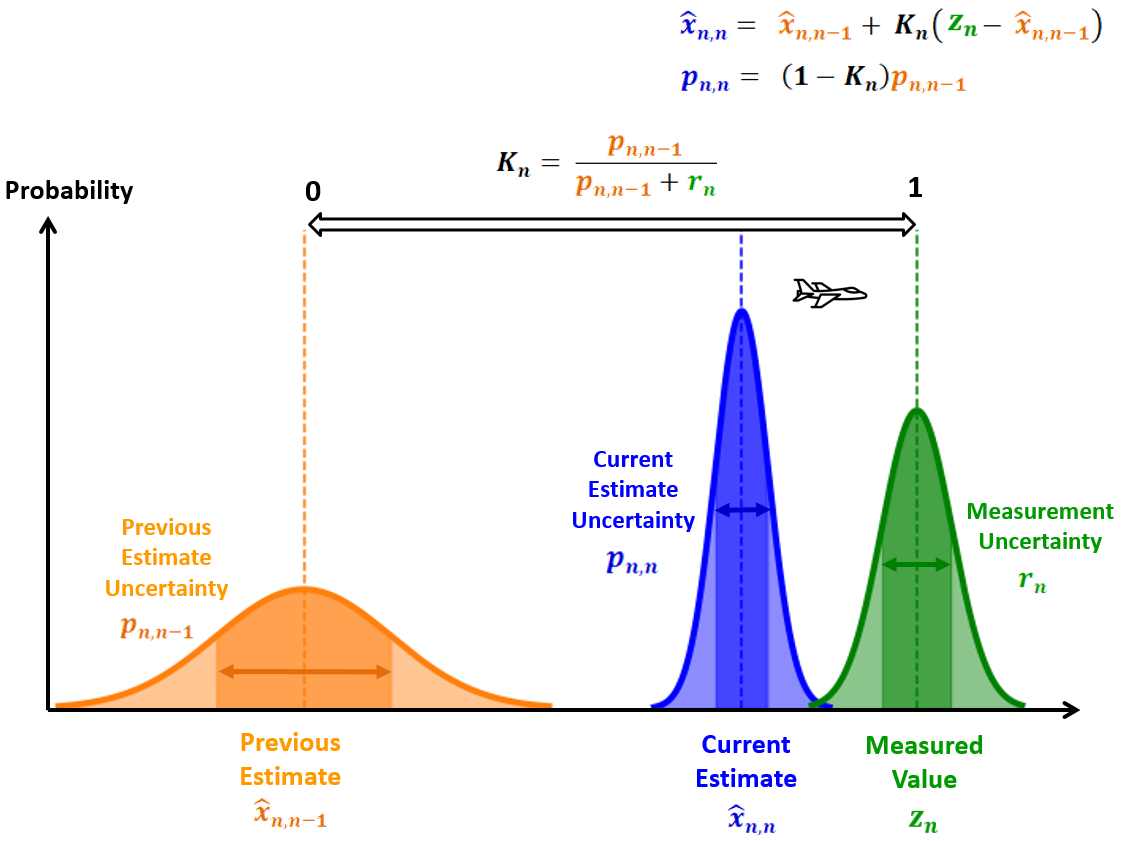
\includegraphics[width=0.65\textwidth]{Figures/Chapter1/HighKalmanGain.png}
	   \label{fig:HighKalmanGain}
	   \vspace{-10pt}
	\end{figure}
\end{frame}
%-----------------------------------------------------
\begin{frame}{Kalman Gain Intuition - Low Kalman Gain}
A high measurement uncertainty relative to the estimate uncertainty would result in a low Kalman Gain (close to 0). Therefore the new estimate would be close to the previous estimate.
    \begin{figure}
	   \centering
   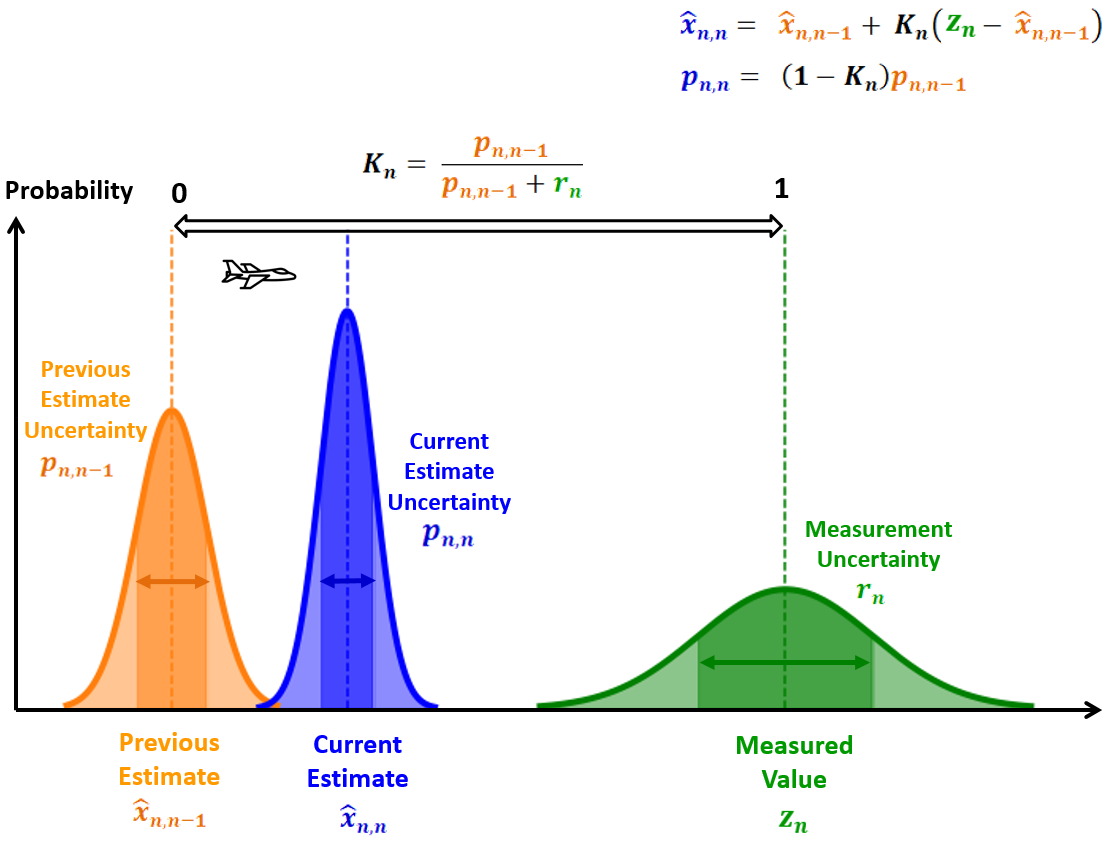
\includegraphics[width=0.7\textwidth]{Figures/Chapter1/LowKalmanGain.png}
	   \label{fig:LowKalmanGain}
	   \vspace{-10pt}
	\end{figure}
\end{frame}

%-----------------------------------------------------
\subsubsection{Example~5: Estimating the Height of the Building}
\begin{frame}{Example~5: Estimating the Height of the Building}
\vspace{-5pt}
We would like to estimate the height of a building using a very imprecise altimeter. The building height doesn't change over time, at least during the short measurement process.

\begin{columns}
    \column{0.5\textwidth}        
    \begin{itemize}
        \item The true building height is 50 meters.
        \item The altimeter measurement error (standard deviation) is 5 meters.
        \item The ten measurements are: 48.54m, 47.11m, 55.01m, 55.15m, 49.89m, 40.85m, 46.72m, 50.05m, 51.27m, 49.95m.
    \end{itemize}
    \textbf{ITERATION ZERO}
    \begin{itemize}
        \item \textbf{Initialization:}
        \begin{itemize}
            \item Estimated build height
            $$\hat{x}_{0,0} = 60m$$
            \item Estimate uncertainty with std. $\sigma = 15m$,
            $$p_{0,0} = 225$$
        \end{itemize}
        \item \textbf{Prediction:}
            \begin{itemize}
                \item Since Dynamic Model is constant
                $$\hat{x}_{1,0}= \hat{x}_{0,0} = 60$$
                \item The extrapolated estimate uncertainty (variance) also doesn't change:
                $$\hat{p}_{1,0}= \hat{p}_{0,0} = 225$$
            \end{itemize}
    \end{itemize}
    \column{0.5\textwidth}        
    \textbf{FIRST ITERATION}
    \begin{itemize}
        \item \textbf{Step~1: Measure:}
            \begin{itemize}
                \item The first measurement is
                $$z_1 = 48.54m$$
                \item The measurement uncertainty (since $\sigma=5$)
                $$r_1 = 25$$
            \end{itemize}
        \item \textbf{Step~2: Update:}
            \begin{itemize}
                \item Kalman gain
                $$K_1 = \frac{p_{1,0}}{p_{1,0} + r_n} = 0.9$$
                \item Estimating the current state:
                $$\hat{x}_{1,1} = \hat{x}_{1,0} + K_1 (z_1 - \hat{x}_{1,0}) = 49.69m$$
                \item  Current estimate uncertainty
                $$p_{1,1} = (1-K_1) p_{1,0} = 22.5$$
            \end{itemize}
        \item \textbf{Step~3: Predict:}
            \begin{itemize}
                \item For constant dynamic model,  
                $$\hat{x}_{2,1} = \hat{x}_{1,1} = 49.69m$$
                $$p_{2,1} = p_{1,1} = 22.5$$
                
            \end{itemize}
    \end{itemize}
\end{columns}
    
    
\end{frame}


%-----------------------------------------------------
\begin{frame}{Example~5: Estimating the Height of the Building --- Results}
\begin{columns}
\vspace{-10pt}
    \column{0.5\textwidth}
    \begin{figure}
	   \centering
	   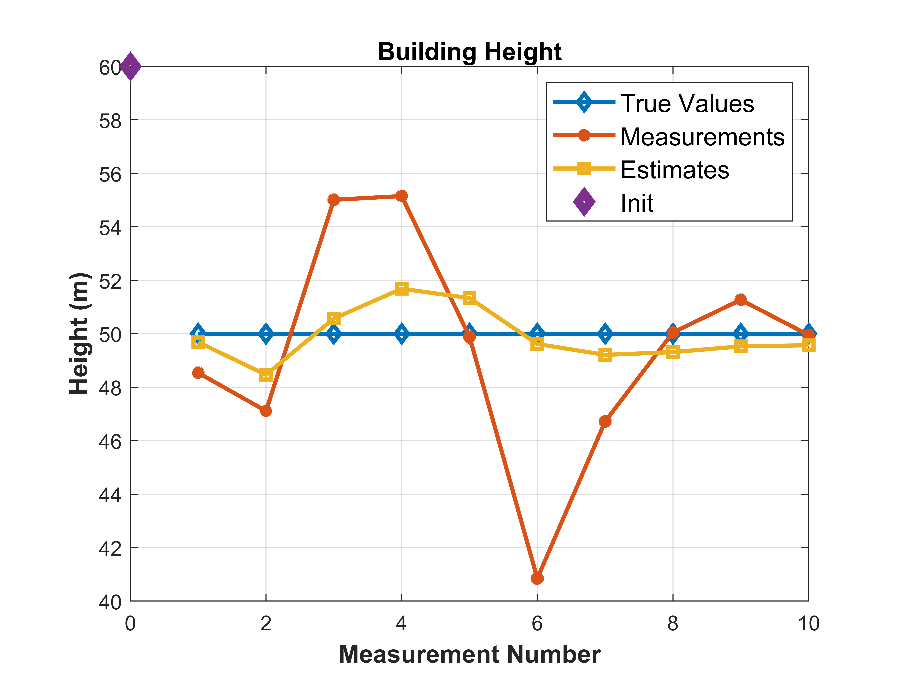
\includegraphics[width=0.6\textwidth]{Figures/Chapter1/ex5_FirstKalmanFilter_H_Estimate.eps}
	   \label{fig:ex5_FirstKalmanFilter_H_Estimate}
	   \vspace{-10pt}
	\end{figure}
	The estimated value converges to about 49.5 meters after 7 measurements.
	
	\begin{figure}
	   \centering
	   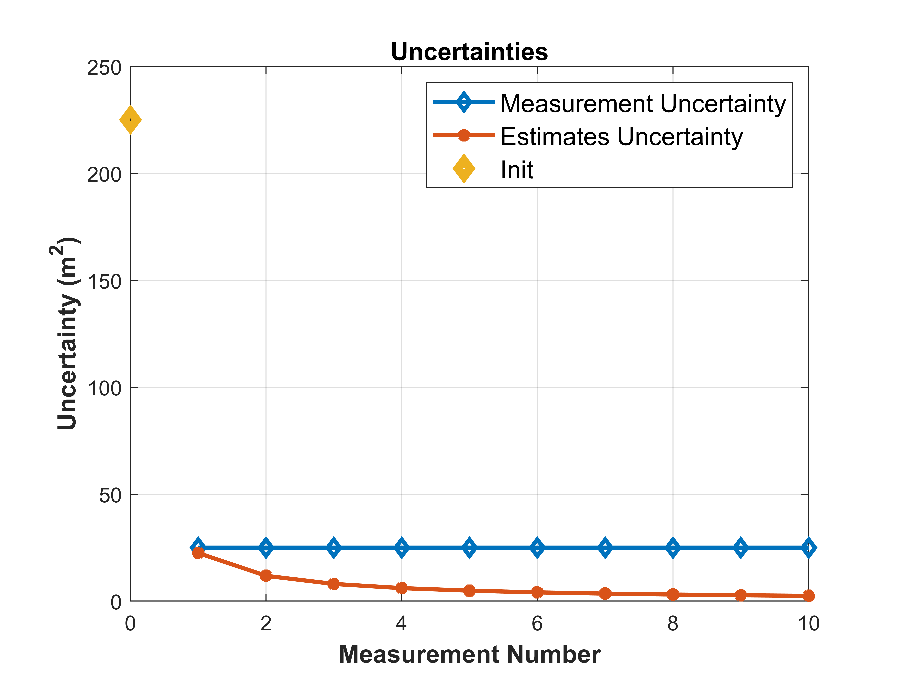
\includegraphics[width=0.6\textwidth]{Figures/Chapter1/ex5_FirstKalmanFilter_Estimate_Uncertainties.eps}
	   \label{fig:ex5_FirstKalmanFilter_Estimate_Uncertainties}
	   \vspace{-10pt}
	\end{figure}
	At 1st filter iteration, the estimate uncertainty is close to the measurement uncertainty and quickly decreases. After 10 measurements, the estimate uncertainty ($\sigma^2$) is 2.47, i.e., the estimate error std is: $\sigma =\sqrt(2.47)=1.57m$.
    \column{0.5\textwidth}
    
    \begin{figure}
	   \centering
	   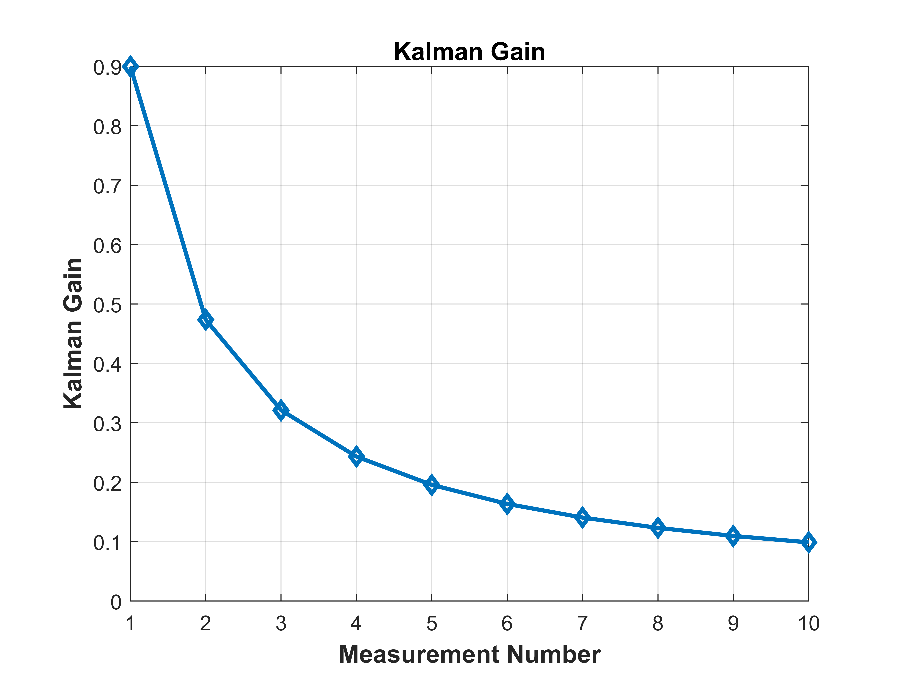
\includegraphics[width=0.8\textwidth]{Figures/Chapter1/ex5_FirstKalmanFilter_KalmanGain.eps}
	   \label{fig:ex5_FirstKalmanFilter__KalmanGain}
	   \vspace{-10pt}
	\end{figure}
	
\textbf{Summary:}	
\begin{itemize}
    \item The Kalman Gain is dynamic and depends on the precision of the measurement device.
    \item The initial value used by the Kalman Filter is not precise. Therefore, the measurement weight in the State Update Equation is high, and the estimate uncertainty is high.
    \item With each iteration, the measurement weight is lower; therefore, the estimate uncertainty is lower.
\end{itemize}
	
\end{columns}    
\end{frame}

%-----------------------------------------------------
\begin{frame}{Example~5: Estimating the Height of the Building --- Results}

One can define accuracy criteria based on the specific application requirements. The
typical accuracy criteria are: \textcolor{blue}{Maximum error, Mean error, Root Mean Square Error (RMSE)}.


Assume that for a building height measurement application, there is a requirement for 95\% confidence.
\begin{columns}
    \column{0.5\textwidth} 
        \begin{figure}
	   \centering
	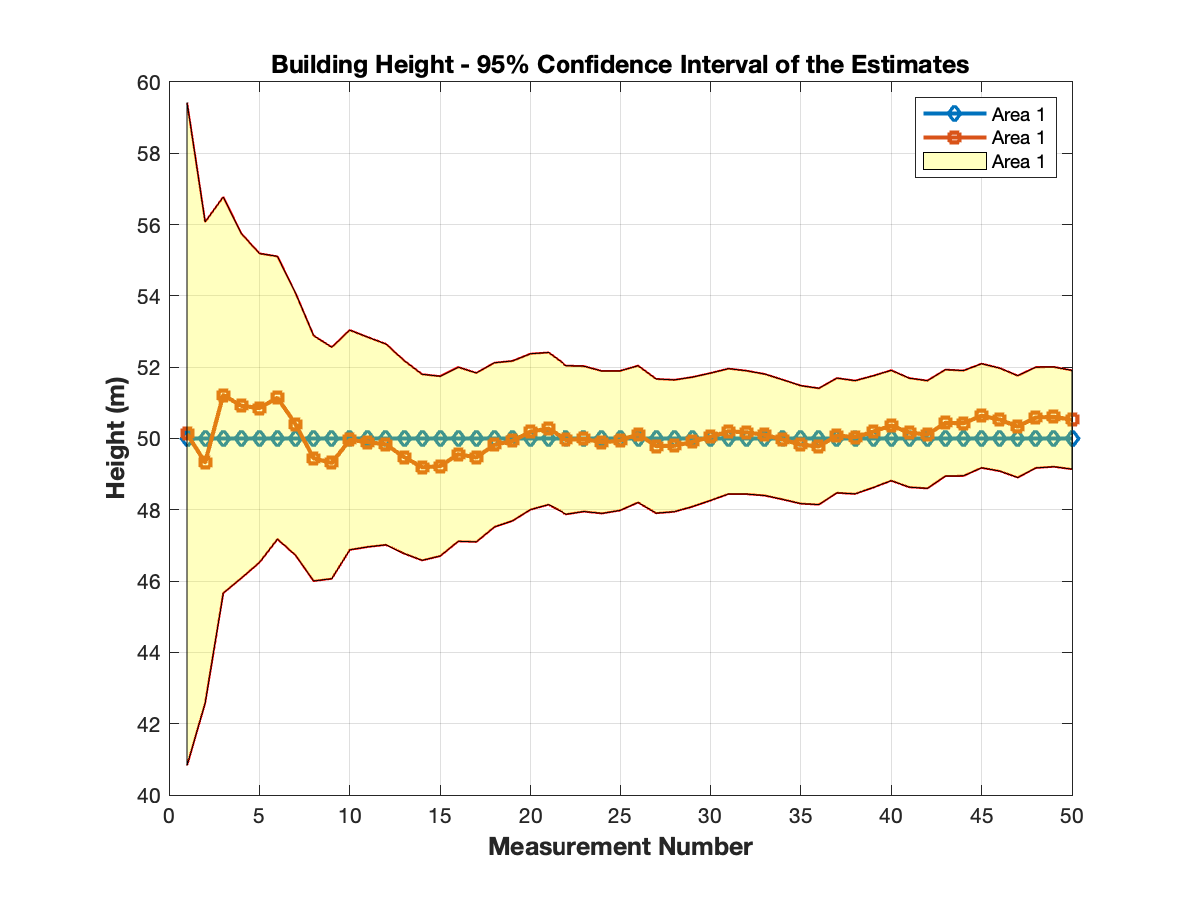
\includegraphics[width=1\textwidth]{Figures/Chapter1/ex5_FirstKalmanFilter_highUncertainty.eps}  \label{fig:ex5_FirstKalmanFilter_highUncertainty}
  \vspace{-20pt}
    \caption{High Uncertainty: $r=5$\,m}
    %\vspace{-5pt}
    \end{figure}
    \column{0.5\textwidth}
        \begin{figure}
	   \centering
	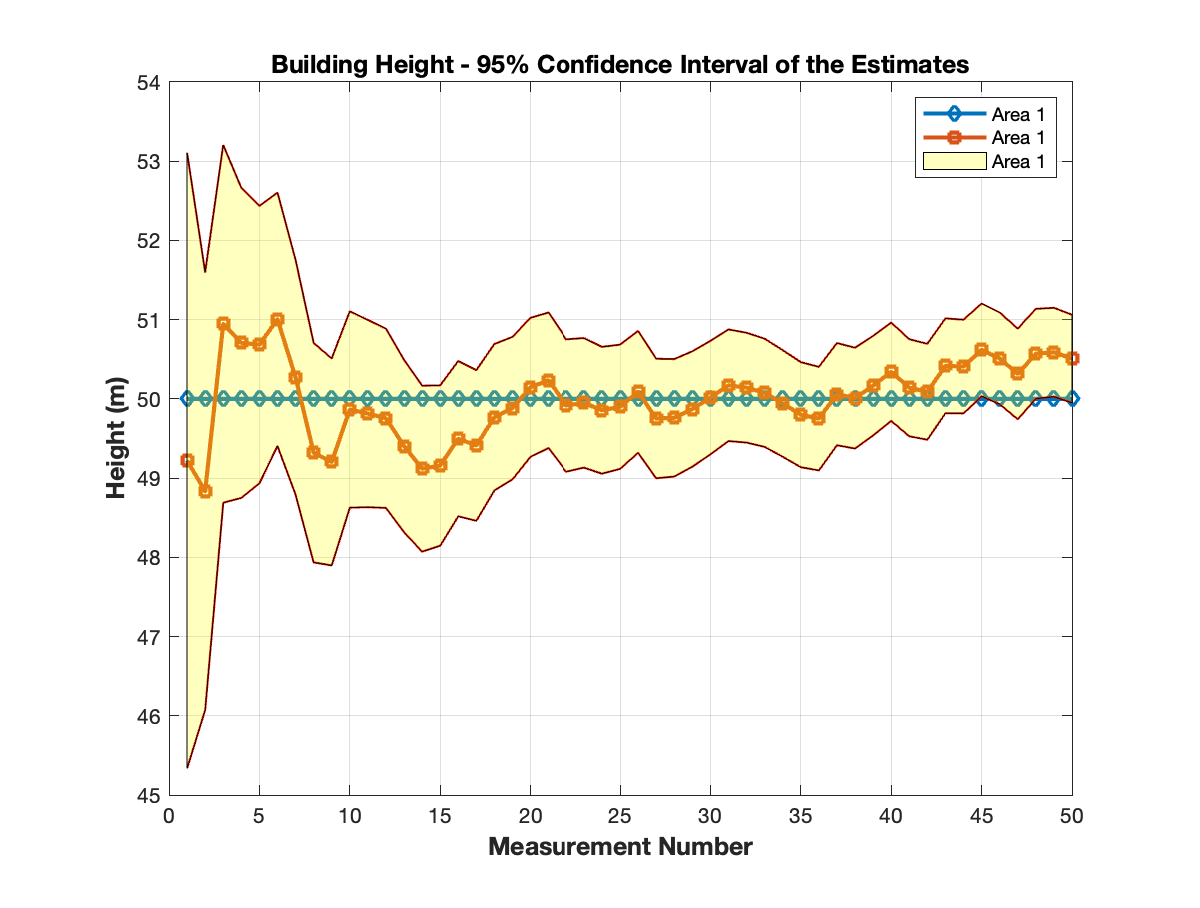
\includegraphics[width=1\textwidth]{Figures/Chapter1/ex5_FirstKalmanFilter_highUncertainty_r2.eps}  \label{fig:ex5_FirstKalmanFilter_highUncertainty}
  \vspace{-20pt}
 \caption{High Uncertainty: $r=2$\,m}
   % \vspace{-5pt}
    \end{figure}
\end{columns}

With measurement uncertainty $r=2$\,m, 2 out of 50 samples slightly exceed the 95\% confidence region; satisfying our requirements of desired estimate uncertainty.

\texttt{\tiny [Code: 1D KF/Ex5\_FirstKalmanFilter.m]}
\end{frame}
%-----------------------------------------------------

\subsection{One-Dimensional Kalman Filter with Process Noise}
\begin{frame}{Complete Model of 1D Kalman Filter including Process Noise}
To complete the one-dimensional Kalman Filter model, we need to add the process noise variable to the Covariance Extrapolation Equation.

\textbf{The Process Noise:}

\begin{itemize}
    \item In the real world, there are uncertainties in the system dynamic model. For example, 
    \begin{itemize}
        \item  When estimating the resistance value of the resistor, we assume a constant dynamic model, i.e., the resistance doesn't change between the measurements. However, the resistance can change slightly due to the fluctuation of the environment temperature.
        
        \item When tracking ballistic missiles with radar, the uncertainty of the dynamic model includes random changes in the target acceleration. 
        
        \item The uncertainties are much more significant for an aircraft due to possible aircraft maneuvers.
        
        \item On the other hand, when estimating the location of a static object using a GPS receiver, the uncertainty of the dynamic model is zero since the static object doesn't move.
    \end{itemize}
    \item The uncertainty of the dynamic model is called the \textcolor{blue}{Process Noise}. In the literature, it is also called \textit{plant noise, driving noise, dynamics noise, model noise, and system noise}. The process noise produces estimation errors.
    
    \item The \textcolor{blue}{Process Noise Variance} is denoted by the letter $q$.
    
    \item The Covariance Extrapolation Equation shall include the Process Noise Variance.
    
    \item For example, the Covariance Extrapolation Equation for constant dynamics is:
    $$p_{n+1,n} = p_{n,n} + q_n$$
    Note: The State Extrapolation Equation and the Covariance Extrapolation Equation depend on the system dynamics.
\end{itemize}
    
\end{frame}



\begin{frame}{Example~6: Estimating the Temperature of the Liquid in a Tank} 
\begin{columns}
    \column{0.5\textwidth}        
    We assume that at a steady state, the liquid temperature is constant. However, some fluctuations in the true liquid temperature are possible. 
    \begin{figure}
        \centering
        
\includegraphics[width=0.5\textwidth]{Figures/Chapter1/ex6_liquid_temperature.png}
        \label{fig:ex6_liquid_temperature}
    \end{figure}
    
    
    We can describe the system dynamics by the following equation:
    
    $$x_n = T + w_n$$
    where\\
    $T$~~is the constant temperature\\
    $w_n$~is a random process noise with variance $q$
    
    \textbf{Assumptions:}
    \begin{itemize}
        \item Tanks true temperature of 50 degrees Celsius
    \end{itemize}
    
    \column{0.5\textwidth}  
    \begin{itemize}
        \item We assume that the model is accurate. Thus, we set the process noise variance, $q=0.0001$.
        \item The measurement error (standard deviation) is 0.1 degrees Celsius.
        \item The measurements are taken every 5 seconds.
        \item The true liquid temperature values at the measurement points are (in degrees Celsius): 49.979, 50.025, 50, 50.003, 49.994, 50.002, 49.999, 50.006, 49.998, and 49.991.
        \item The measurements are (in degrees Celsius): 49.95, 49.967, 50.1, 50.106, 49.992, 49.819, 49.933, 50.007, 50.023, and 49.99.
    \end{itemize}
\end{columns}

    
\end{frame}

%-----------------------------------------------------
\subsubsection{Example~6: Estimating the Temperature of the Liquid in a Tank} 
\begin{frame}{Example~6: Estimating the Temperature of the Liquid in a Tank} 
\begin{columns}
    \column{0.5\textwidth}        
       \textbf{ITERATION ZERO}
    \begin{itemize}
        \item \textbf{Initialization:}
        \begin{itemize}
            \item We don't know the true temperature of the liquid in a tank; our estimate (or guess) is
            $$\hat{x}_{0,0} = 10^o C$$
            \item Estimate uncertainty with std. $\sigma = 100$,
            $$p_{0,0} = \sigma^2 = 10,000$$
        \end{itemize}
        \item \textbf{Prediction:}
            \begin{itemize}
                \item Since our model has constant dynamics, the predicted estimate is equal to the current estimate:
                $$\hat{x}_{1,0}= \hat{x}_{0,0} = 10^oC$$
                \item The extrapolated estimate uncertainty (variance):
                $$\hat{p}_{1,0}= \hat{p}_{0,0} + q = 10000 + 0.0001$$
            \end{itemize}
    \end{itemize}
    \column{0.5\textwidth}
        \textbf{FIRST ITERATION}
    \begin{itemize}
        \item \textbf{Step~1: Measure:}
            \begin{itemize}
                \item The first measurement is
                $$z_1 = 49.95^oC$$
                
                \item The measurement uncertainty (since $\sigma=0.1$)
                $$r_1 = 0.01$$
            \end{itemize}
        \item \textbf{Step~2: Update:}
            \begin{itemize}
                \item Kalman gain
                $$K_1 = \frac{p_{1,0}}{p_{1,0} + r_n} = 0.999999~[\approx 1]$$
                \item Estimating the current state:
                $$\hat{x}_{1,1} = \hat{x}_{1,0} + K_1 (z_1 - \hat{x}_{1,0}) = 49.95^o C$$
                \item  Current estimate uncertainty
                $$p_{1,1} = (1-K_1) p_{1,0} = 0.01$$
            \end{itemize}
        \item \textbf{Step~3: Predict:}
            \begin{itemize}
                \item For constant dynamic model,  
                $$\hat{x}_{2,1} = \hat{x}_{1,1} = 49.95^o C$$
                $$p_{2,1} = p_{1,1} + q = 0.0101$$
                
            \end{itemize}
    \end{itemize}
\end{columns}
    
\end{frame}

%-----------------------------------------------------
\begin{frame}{Example~6: Estimating the Temperature of the Liquid in a Tank --- Results} 
\begin{columns}
    \column{0.5\textwidth}
    \begin{itemize}
        \item The estimated value converges toward the true value.
        \item The estimate uncertainty quickly goes down. After 10 measurements, the estimate uncertainty is $\sigma^2=0.0013$, i.e., the estimate error std is: $\sigma=0.036^oC$.
        \item So we can say that the liquid temperature estimate is: $49.988 \pm 0.036^oC$.
        \item \textbf{Summary:} Although the system dynamics include a random process noise, the Kalman Filter can provide a good estimation.
    \end{itemize}
    \vspace{-10pt}
    \begin{figure}
        \centering
        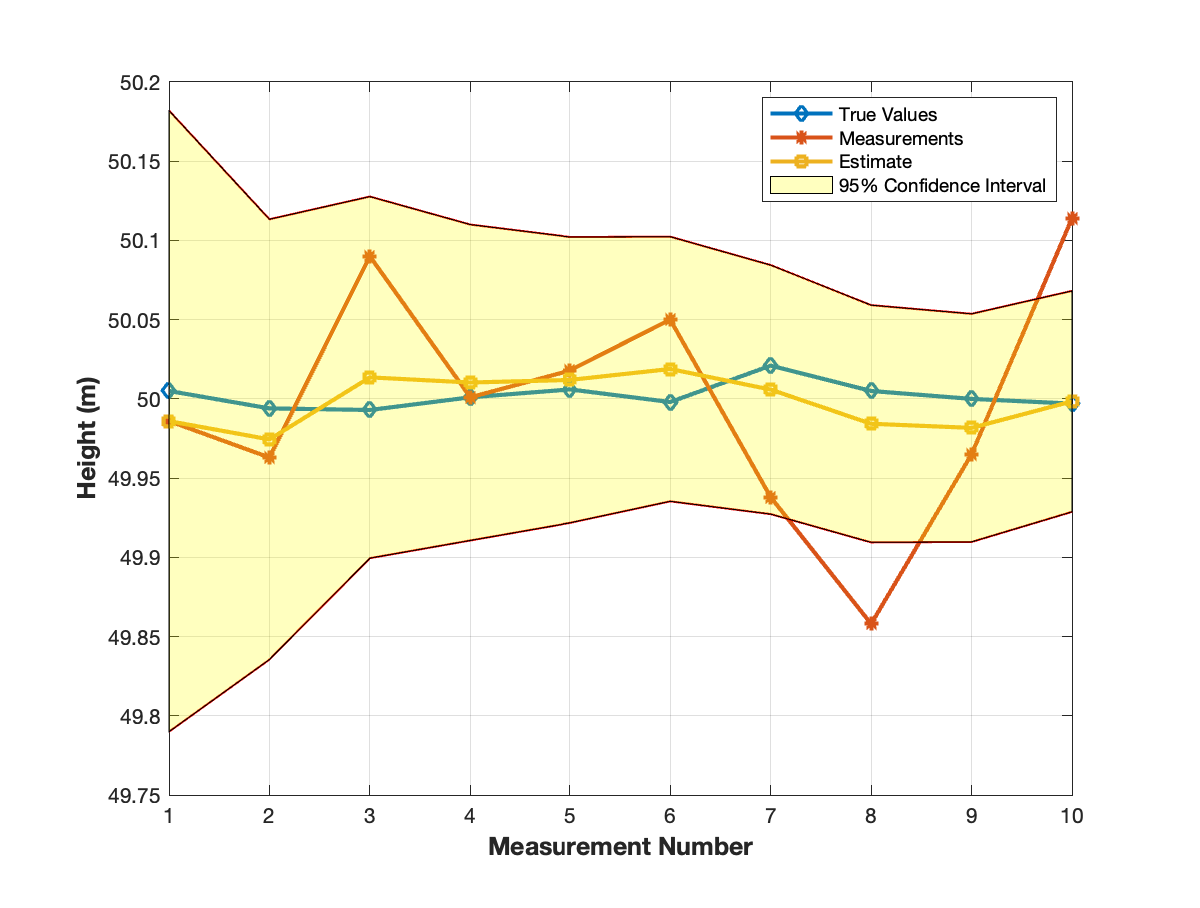
\includegraphics[width=0.8\textwidth]{Figures/Chapter1/ex6_KalmanFilter_ProcessNoise_95CI.eps}
\label{fig:ex6_KalmanFilter_ProcessNoise_95CI}
    \end{figure}
    \column{0.5\textwidth}
    \begin{figure}
        \centering
        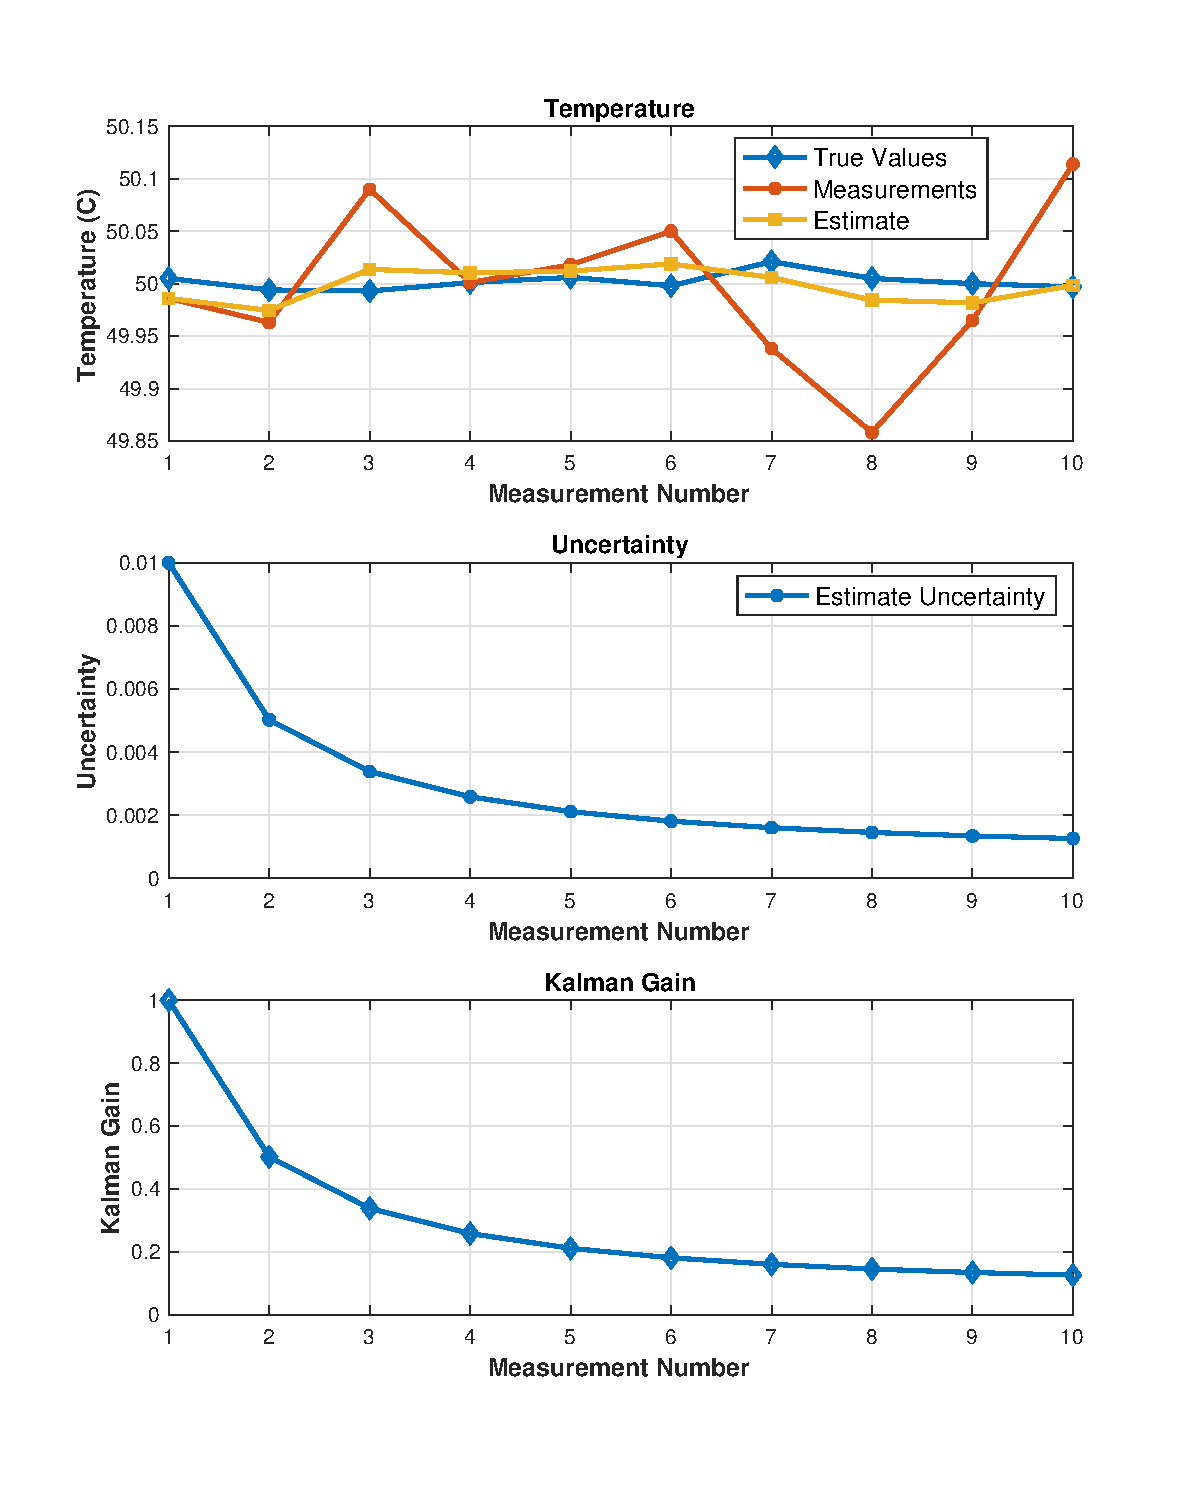
\includegraphics[width=1\textwidth]{Figures/Chapter1/ex6_KalmanFilter_ProcessNoise.eps}
        \label{fig:ex6_KalmanFilter_ProcessNoise}
        \vspace{-25pt}
    \end{figure}
    \texttt{\tiny [Code: 1D KF/Ex6\_KalmanFilter\_ProcessNoise.m]}
\end{columns}
\end{frame}
%----------------------------------------------------- 
\subsubsection{Example~7: Estimating the Temperature of a Heating Liquid in a Tank I} 
\begin{frame}{Example~7: Estimating the Temperature of a Heating Liquid in a Tank I} 
\begin{columns}
    \column{0.5\textwidth}        
    \begin{itemize}
        \item Let's estimate the temperature of a liquid in a tank as in Example~6. However, in this case, the dynamic model of the system is not constant--- the liquid is heating at a rate of $0.1^oC/sec$.
        \item Parameters are same as in Example~6.
        \item The dynamic model of the system is constant. Although the true dynamic model of the system is not constant (since the liquid is heating), we treat the system as a system with a constant dynamic model (the temperature doesn't change)
        \item The true liquid temperature values at the measurement points are: 50.479, 51.025, 51.5, 52.003, 52.494, 53.002, 53.499, 54.006, 54.498, and 54.991.
        \item The measurements are: 50.45, 50.967, 51.6, 52.106, 52.492, 52.819, 53.433, 54.007, 54.523, and 54.99.
        \item Kalman Filter has failed to provide a reliable estimation as there is a lag error in the estimation.
    \end{itemize}    
    \column{0.5\textwidth}
    \vspace{-5pt}
    \begin{figure}
        \centering
        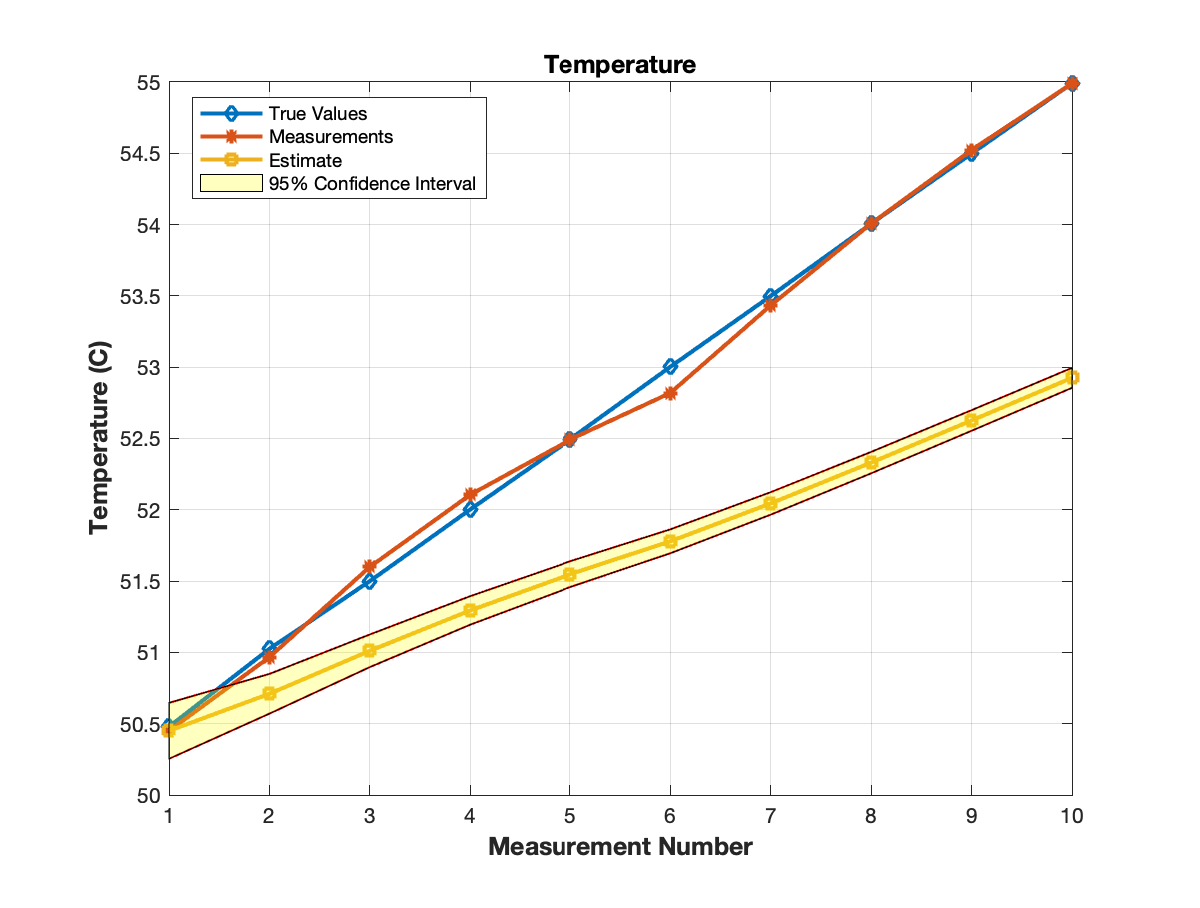
\includegraphics[width=0.7\textwidth]{Figures/Chapter1/ex7_KalmanFilter_ProcessNoise_I.eps}
        \label{fig:ex7_KalmanFilter_ProcessNoise_I}
        \vspace{-10pt}
    \end{figure}
    \begin{itemize}
     \item \textbf{Two Reason for the constant lag error:}  
    % The lag error is caused by the wrong dynamic model and process model definitions.
        \begin{itemize}
            \item The dynamic model doesn't fit the case.
            \item  Process noise is very low ($q=0.0001$) while the true temperature fluctuations are much more significant.
        \end{itemize}
        \item Two possible ways to fix the lag error:    
            \begin{itemize}
                \item If we know that the liquid temperature can change linearly, we can define a new model that considers that. \textit{What of the temperature change cannot be modeled?}
                \item If the model is not well defined, we can adjust the process model reliability by increasing the process noise ($q$).
            \end{itemize}
    \end{itemize}
            \texttt{\tiny [Code: 1D KF/Ex7\_KalmanFilter\_ProcessNoise\_I.m]}
\end{columns}
\end{frame}

%-----------------------------------------------------
\subsubsection{Example~8: Estimating the Temperature of a Heating Liquid in a Tank II}
\begin{frame}{Example~8: Estimating the Temperature of a Heating Liquid in a Tank II} 
\begin{columns}
    \column{0.5\textwidth}        
    This example is similar to the previous example, with only one change. Since our process is not well-defined, we increase the process uncertainty ($q$) from 0.0001 to 0.15.
    \begin{itemize}
        \item Due to the high process uncertainty, the measurement weight is much higher than the weight of the estimate. Thus, the Kalman Gain is high, and it converges to 0.94.
        \item We can eliminate the lag error by setting a high process uncertainty. However, since our model is not well-defined, we get noisy estimates that are almost equal to the measurements, and we miss the goal of the Kalman Filter.
        \item The best Kalman Filter implementation would involve a model that is very close to reality, leaving little room for process noise. However, a precise model is not always available 
    \end{itemize}
    
    \column{0.5\textwidth}   
    \begin{figure}
        \centering
        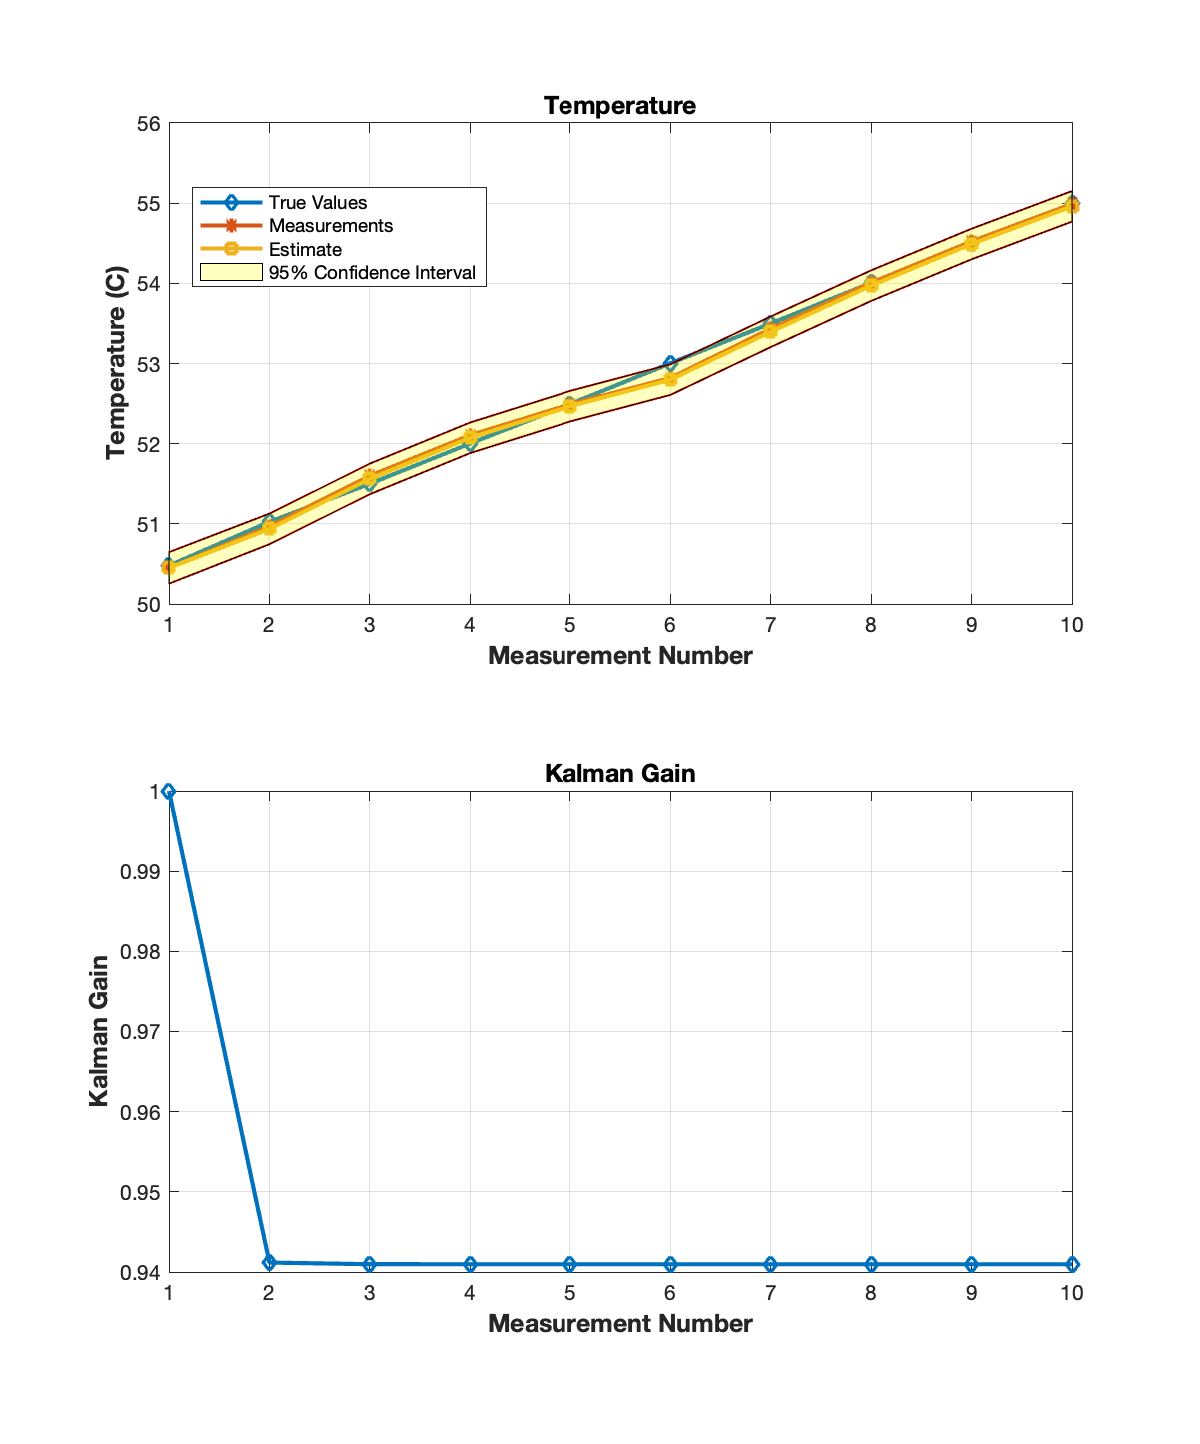
\includegraphics[width=1\textwidth]{Figures/Chapter1/ex8_KalmanFilter_ProcessNoise_II.eps}
    \label{fig:ex8_KalmanFilter_ProcessNoise_II}
    \vspace{-15pt}
    \end{figure}
        \texttt{\tiny [Code: 1D KF/Ex8\_KalmanFilter\_ProcessNoise\_II.m]}
\end{columns}
    
\end{frame}

\section{Part 2: Multidimensional (Multivariate) Kalman Filter}

\begin{frame}
   \frametitle{Part 2: Multidimensional (Multivariate) Kalman Filter}
		
		\textbf{Objectives}
				
		\begin{itemize}
			\item Kalman Filter with matrix notation for designing a multivariate Kalman Filter
            \item Linear Kalman Filter (LKF): assumes that the system dynamics are linear
			\item Mathematical derivation of Kalman Filter equations, dynamic systems modeling, and two numerical examples
		\end{itemize}
		
		\vspace{10pt}
		
		% \begin{exampleblock}{}
  % {\small ``The road to learning by precept is long, by example short and effective.''}
  % \vskip3mm
  % \hspace*\fill{\small--- Lucius Seneca}
% \end{exampleblock}


% 		\begin{framed}
% 		\begin{center}
% 		\textbf{Designing reliable systems with guaranteed performance under time dependent varying wireless channel chracteristics }
% 		\end{center}
% 		\end{framed}
\end{frame}


\subsection{Introduction}
\begin{frame}{Introduction}
\begin{columns}
    \column{0.5\textwidth} 
        \begin{itemize}
            \item Until now, we have been looking at 1D processes, like estimating the liquid temperature.
            \item But many dynamic processes have 2, 3, or even more dimensions.
            \item \textbf{Ex1:} The state vector that describes the airplane's position in space is 3D:
            \begin{equation*}
            \centering
            \begin{bmatrix}
            x\\
            y\\
            z\\
            \end{bmatrix}
            \end{equation*}
            \item \textbf{Ex2:} The state vector that describes the airplane position and velocity is 6-D:
            \begin{equation*}
            \centering
            \begin{bmatrix}
            x\\
            y\\
            z\\
            \dot{x}\\
            \dot{y}\\
            \dot{z}\\
            \end{bmatrix}
            \end{equation*}
        \end{itemize}
    \column{0.5\textwidth} 
    \begin{itemize}
        \item \textbf{Ex3:} The state vector that describes the airplane position, velocity, and acceleration is nine-dimensional:
            \begin{equation*}
            \centering
            \begin{bmatrix}
            x\\
            y\\
            z\\
            \dot{x}\\
            \dot{y}\\
            \dot{z}\\
            \ddot{x}\\
            \ddot{y}\\
            \ddot{z}\\
            \end{bmatrix}
            \end{equation*}
        
        \begin{figure}
            \centering
            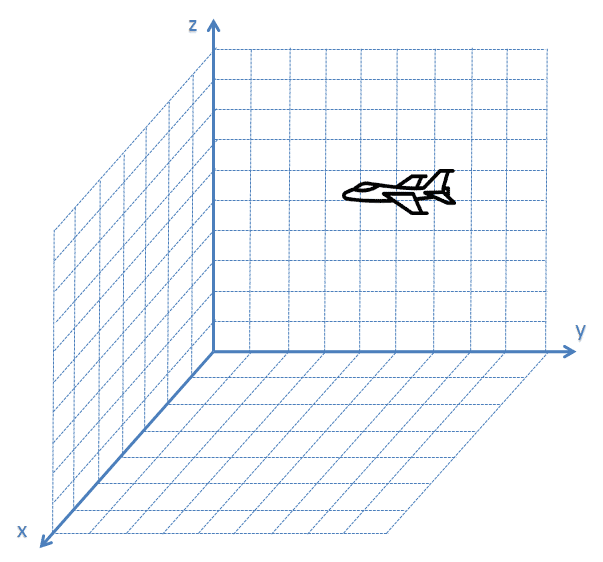
\includegraphics[width=0.5\textwidth]{Figures/Chapter2/3Dfighter.png}
            \label{fig:3Dfighter}
            \vspace{-5pt}
        \end{figure}
    \end{itemize}
\end{columns}
\end{frame}
%-------------------------------------------------
\begin{frame}{Introduction}
    % \begin{columns}
        % \column{0.5\textwidth}
    \begin{itemize}
        
    \item Assuming a constant acceleration dynamic model, we can describe the extrapolated airplane state at time $n$ by nine motion equations:
        
    \begin{align*}
     x_n = & x_{n-1} + \dot{x}_{n-1} \Delta t + \frac{1}{2}\ddot{x}_{n-1}\Delta t^2\\\nonumber
     y_n = & y_{n-1} + \dot{y}_{n-1} \Delta t + \frac{1}{2}\ddot{y}_{n-1}\Delta t^2\\\nonumber
     z_n = & z_{n-1} + \dot{z}_{n-1} \Delta t + \frac{1}{2}\ddot{z}_{n-1}\Delta t^2\\\nonumber
     \dot{x}_n = & \dot{x}_{n-1} + \ddot{x}_{n-1} \Delta t\\\nonumber
     \dot{y}_n = & \dot{y}_{n-1} + \ddot{y}_{n-1} \Delta t\\\nonumber
     \dot{z}_n = & \dot{z}_{n-1} + \ddot{z}_{n-1} \Delta t\\\nonumber
     \ddot{x}_{n} = & \ddot{x}_{n-1}\\\nonumber
     \ddot{y}_{n} = & \ddot{y}_{n-1}\\\nonumber
     \ddot{z}_{n} = & \ddot{z}_{n-1}\\\nonumber
    \end{align*}
        % \column{0.5\textwidth}
    \item Common practice to describe a multidimensional process with a single equation in matrix form.
    
    \item Second, computers are highly efficient at matrix calculations. Implementing the Kalman Filter in matrix form yields faster computation run time.
    % \end{columns}
    \end{itemize}
\end{frame}

%%%%%%%%%%%%%%%%%%%%%%%%%%%%%%%%%%%%%%%%%%%%%%%%%%%%%%%%%%%%%%%%%%%%%%%%%%%%%%%%%%%%%%%%%%%%%%%%%%%%%%%%%%%%%%%%%%%%%%%%%%%
%-------------------------------------------------
\subsection{Essential Background II}
\subsubsection{Expectation Algebra}
\begin{frame}{The Background Break - Expectation Algebra}
    % \begin{columns}
        % \column{0.5\textwidth}
        The necessary mathematical background for Kalman Filter:
            \begin{itemize}
                \item Matrix Operations: Vector/matrix addition and multiplication, transpose, Matrix inverse, Symmetric matrices
                \item Expectation Algebra
                \item Multivariate Normal Distribution (Covariance and Covariance Matrices)
            \end{itemize}
        \textbf{Expectation Algebra}
        \begin{itemize}
            \item The expectation of a random variable $X$ equal the mean of $X$: $E(X)=\mu_X$.
        \end{itemize}
         \begin{table}[]
            \centering
            \begin{tabular}{ll}
                \toprule
                \textbf{Rule} & \textbf{Notes} \\
                \toprule
                $E(X) = \mu_X = \sum x p(x)$ & $p(x)$ is PDF of $x$ \\
                $E(a) = a$ & $a$ is constant\\
                $E(aX) = aE(x)$ & $--$\\
                $E(a\pm X) = a\pm E(x)$ & $--$\\
                $E(a\pm bX) = a\pm bE(x)$ & $b$ is constant\\
                $E(X\pm Y) = E(x) \pm E(Y)$ & $Y$ is another R.V.\\
                $E(XY) = E(X)E(Y)$ & $X, Y$ are independent\\
                \bottomrule
            \end{tabular}
            \caption{Expectation Rules}
            \label{tab:ExpectationRules}
        \end{table}
        % \column{0.5\textwidth}
    % \end{columns}
\end{frame}

%-------------------------------------------------

\begin{frame}{The Background Break - Expectation Algebra}
    % \begin{columns}
        % \column{0.5\textwidth}
        The following table includes the variance and covariance expectation rules.
        \begin{itemize}
            \item Variance of a R.V. $X$: $V(X) = E\left((X-\mu_X)^2\right)$
            \item Covariance of R.V. $X$ and $Y$: $COV(X,Y) = E\left((X-\mu_X)(Y-\mu_Y)\right)$
        \end{itemize}
         \begin{table}[]
            \centering
            \begin{tabular}{ll}
                \toprule
                \textbf{Rule} & \textbf{Notes} \\
                \toprule
                $V(a) = 0$ & Variance of a constant $a$\\[0.7em]
                $V(a\pm X) = V(X)$ & Variance of $X$\\[0.7em]
                $V(X) = E(X^2) - \mu_X^2$ & $--$\\[0.7em]
                $V(a\pm X) = a^2 V(X)$ & $a$ is constant\\[0.7em]
                $COV(X,Y) =E(XY) + \mu_X \mu_Y$ & Covariance of $X$ and $Y$\\[0.7em]
                $COV(X,Y) = 0$ & If $X$ and $Y$ are Independent\\[0.7em]
                $V(X\pm Y) = V(X) + V(Y) \pm 2COV(X,Y)$ & \\[0.7em]
                $V(XY) \neq V(X) V(Y)$ & \\[0.7em]
                \bottomrule
            \end{tabular}
            \caption{Variance and Covariance Expectation Rules}
            \label{tab:Var_CoVar_Rules}
        \end{table}
\end{frame}

%-------------------------------------------------
\begin{frame}{The Background Break - Multivariate Normal Distribution}
\begin{itemize}
\item Introduction to the Kalman Filter: 
    \begin{itemize}
        \item The Kalman Filter output is a random variable.
        \item The mean of the random variable is the state estimate.
        \item The variance represents the estimation uncertainty.
        \item It provides us with the estimate and the level of confidence of its estimate.
    \end{itemize}
\item One-dimensional Kalman Filter equations include four uncertainty variables:
    \begin{enumerate}
        \item \(p_{n,n}\) is the variance of an estimate (the current state).
        \item \(p_{n+1,n}\) is the variance of a prediction (the next state).
        \item \(r_n\) is the measurement variance.
        \item \(q\) is the process noise.
    \end{enumerate}

\item Multivariate Kalman Filter
    \begin{itemize}
        \item Describes the system state by a vector with more than one variable.
        \item For example, object’s position on the plane: \[x = \begin{bmatrix} x \\ y \end{bmatrix}\] 
        \item The Kalman Filter output is a multivariate random variable.
        \item A covariance matrix describes the squared uncertainty of the multivariate random variable.
    \end{itemize}

\item Uncertainty variables of multivariate Kalman Filter
    \begin{itemize}
        \item The uncertainty variables are represented by covariance matrices:
        \begin{enumerate}
            \item \(P_{n,n}\) describes the squared uncertainty of an estimate.
            \item \(P_{n+1,n}\) describes the squared uncertainty of a prediction.
            \item \(R_n\) describes the squared measurement uncertainty.
            \item \(Q\) describes the process noise.
        \end{enumerate}
    \end{itemize}
\end{itemize}    
\end{frame}
%-------------------------------------------------
\subsubsection{Covariance}
\begin{frame}{The Background Break - Multivariate Normal Distribution}
    \begin{itemize}
        \item Covariance is a measure of the strength of the correlation between two or more sets of random variates.
        \item On the x-y plane, variance in measurements exists due to random error.
    \end{itemize}
        \begin{itemize}
            \item \textbf{Uncorrelated measurements:}
            \begin{itemize}
                \item The x and y values don't depend on each other. The covariance of x and y equals zero.
                \item For the blue data set, a circular distribution shape indicates equal variance.
                \item For the red data set, an elliptic distribution shape indicates greater variance in x values.
            \end{itemize}
            \item \textbf{Correlated measurements:}
            \begin{itemize}
                \item Dependency exists between x and y values.
                \item For the green data set, positive correlation and covariance due to concurrent increase.
                \item For the cyan data set, negative correlation and covariance due to inverse changes.
            \end{itemize}
        \end{itemize}
    \begin{figure}
        \centering
    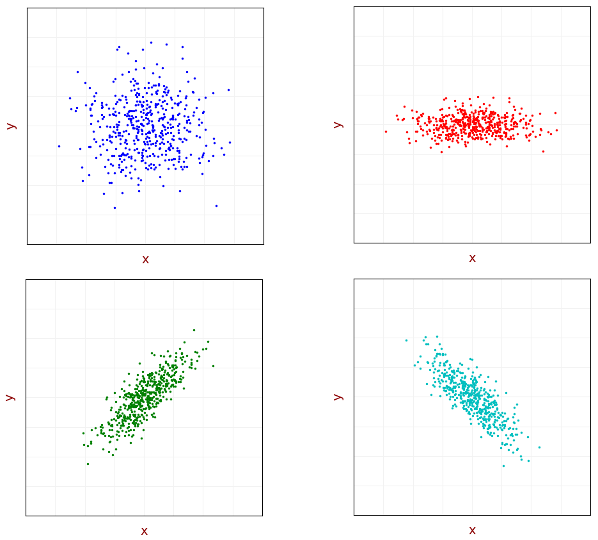
\includegraphics[width=0.4\textwidth]{Figures/Background2/CovarianceIllustration.png}
        \caption{Examples of different measurement sets.}
    \end{figure}

\end{frame}
%--------------------------------------------------------------------
\begin{frame}{The Background Break - Covariance}
The covariance between population $X$ and population $Y$ with size $N$
    \begin{align}
       \text{COV} (X, Y) & = \frac{1}{N} \sum_{i=1}^{N} (x_i - \mu_x)(y_i - \mu_y)\nonumber\\ & = \frac{1}{N} \sum_{i=1}^{N} (x_i y_i) - \mu_x \mu_y \nonumber
    \end{align}
The covariance of a sample with size $N$ is normalized by $N - 1$
    \begin{align}
     \text{COV} (X, Y) & = \frac{1}{N - 1} \sum_{i=1}^{N} (x_i - \mu_x)(y_i - \mu_y)\nonumber \\ &= \frac{1}{N - 1} \left( \sum_{i=1}^{N} x_i y_i \right) - \frac{N}{N - 1} \mu_x \mu_y \nonumber\\
     & = \frac{1}{N - 1}{\mathbf{x}^T y - \frac{N}{N - 1} \mu_x \mu_y}\nonumber \quad [\text{In vector notation}]\\
     & = \frac{1}{N - 1}\mathbf{x}^T y \quad [\text{For a zero-mean random variable}]\nonumber
     \end{align}
\end{frame}

%-------------------------------------------------
\subsubsection{Covariance Matrix}
\begin{frame}{The Background Break - Covariance Matrix}
A covariance matrix is a square matrix that represents the covariance between each
pair of elements in a given multivariate random variable.

For a two-dimensional random variable, the covariance matrix is given by
\begin{equation*}
    \Sigma = 
    \begin{bmatrix}
        \sigma_{xx} & \sigma_{xy} \\
        \sigma_{yx} & \sigma_{yy}
    \end{bmatrix}
    =
    \begin{bmatrix}
        \sigma^2_{x} & \sigma_{xy} \\
        \sigma_{yx} & \sigma^2_{y}
    \end{bmatrix}
    =
    \begin{bmatrix}
        \text{VAR}(x) & \text{COV}(x, y) \\
        \text{COV}(y, x) & \text{VAR}(y)
    \end{bmatrix}
\end{equation*}
Note that the off-diagonal entries of the covariance matrix are equal since $\text{COV}(x, y) =
\text{COV}(y, x)$. If $x$ and $y$ are uncorrelated, the off-diagonal entries of the covariance
matrix are zero.


\textbf{Properties of the covariance matrix:}
\begin{itemize}
    \item The diagonal entries of this covariance matrix are the variances of the components of the multivariate random variable:
    $$\Sigma_{ii} = \sigma^2_{i}$$
    \item Since the diagonal entries are all non-negative, the trace (the sum of diagonal entries) of this covariance matrix is non-negative:
    $$\text{tr}(\mathbf{\Sigma}) = \sum_{i=1}^{n} \Sigma_{ii} \geq 0$$ 
    \item Since \(\Sigma_{ij} = \sigma_{ij} = \sigma_{ji} = \Sigma_{ji}\), the covariance matrix is symmetric:
    $$\mathbf{\Sigma} = \mathbf{\Sigma^T}$$
    \item The covariance matrix is \textbf{positive semidefinite}. The matrix \(\mathbf{A}\) is called positive semidefinite if \(\mathbf{v}^T \mathbf{A} \mathbf{v} \geq 0\), for any vector \(v\). \textbf{The eigenvalues of \(\mathbf{A}\) are non-negative}.
\end{itemize}

\end{frame}
%-------------------------------------------------
\subsubsection{Covariance Matrix and Expectation}
\begin{frame}{The Background Break - Expectation Algebra - Covariance Matrix and Expectation}
\begin{itemize}
    \item Assume a vector $\mathbf{x}$ with $k$ elements:
        \begin{equation*}
            \centering
            \mathbf{x}=\begin{bmatrix}
            x_1\\
            x_2\\
            \vdots\\
            x_k\\
            \end{bmatrix}
            \end{equation*}
    \item The covariance matrix of the vector $\mathbf{x}$ is:
            \begin{align*}
            \centering
            COV(\mathbf{x}) = & E\left((\mathbf{x} -\mathbf{\mu}_x)(\mathbf{x} -\mathbf{\mu}_x)^T\right)\\
            = & E\left(\begin{bmatrix}
            (x_1-\mu_{x_1})\\
            (x_2-\mu_{x_2})\\
            \vdots\\
            (x_k-\mu_{x_k})\\
            \end{bmatrix}
            \Big[(x_1-\mu_{x_1})~~(x_2-\mu_{x_2})~~\cdots~~ (x_k-\mu_{x_k})\Big]
            \right)
            \end{align*}
\end{itemize}
\end{frame}


%-------------------------------------------------------
\subsubsection{Multivariate Normal Distribution}
\begin{frame}{The Background Break - Multivariate Normal Distribution}

Univariate Gaussian distribution:
$$p(x|\mu, \sigma) = \frac{1}{\sqrt{2\pi\sigma^2}} \exp\left(-\frac{(x - \mu)^2}{2\sigma^2}\right)$$

The $n$ - dimensional multivariate normal distribution:
$$p(\mathbf{x}|\boldsymbol{\mu},\mathbf{\Sigma)} = \frac{1}{\sqrt{(2\pi)^n |\mathbf{\Sigma}|}} \exp\left(-\frac{1}{2}(\mathbf{x} - \boldsymbol{\mu})^T \mathbf{\Sigma}^{-1} (\mathbf{x} - \boldsymbol{\mu})\right)$$
\begin{itemize}
    \item $\mathbf{x}$ is an \(n\)-dimensional random vector,
    \item $\boldsymbol{\mu}$ is an \(n\)-dimensional mean vector,
    \item $\boldsymbol{\Sigma}$ is a square \(n \times n\) covariance matrix,
    \item $\boldsymbol{\Sigma}^{-1}$ is the inverse of the covariance matrix,
    \item $|\boldsymbol{\Sigma}| \equiv \det(\boldsymbol{\Sigma})$ is the determinant of ${\boldsymbol {\Sigma }}$.
\end{itemize}
\vspace{-10pt}
\begin{columns}
        \column{0.5\textwidth} 
            \begin{figure}
    \centering
    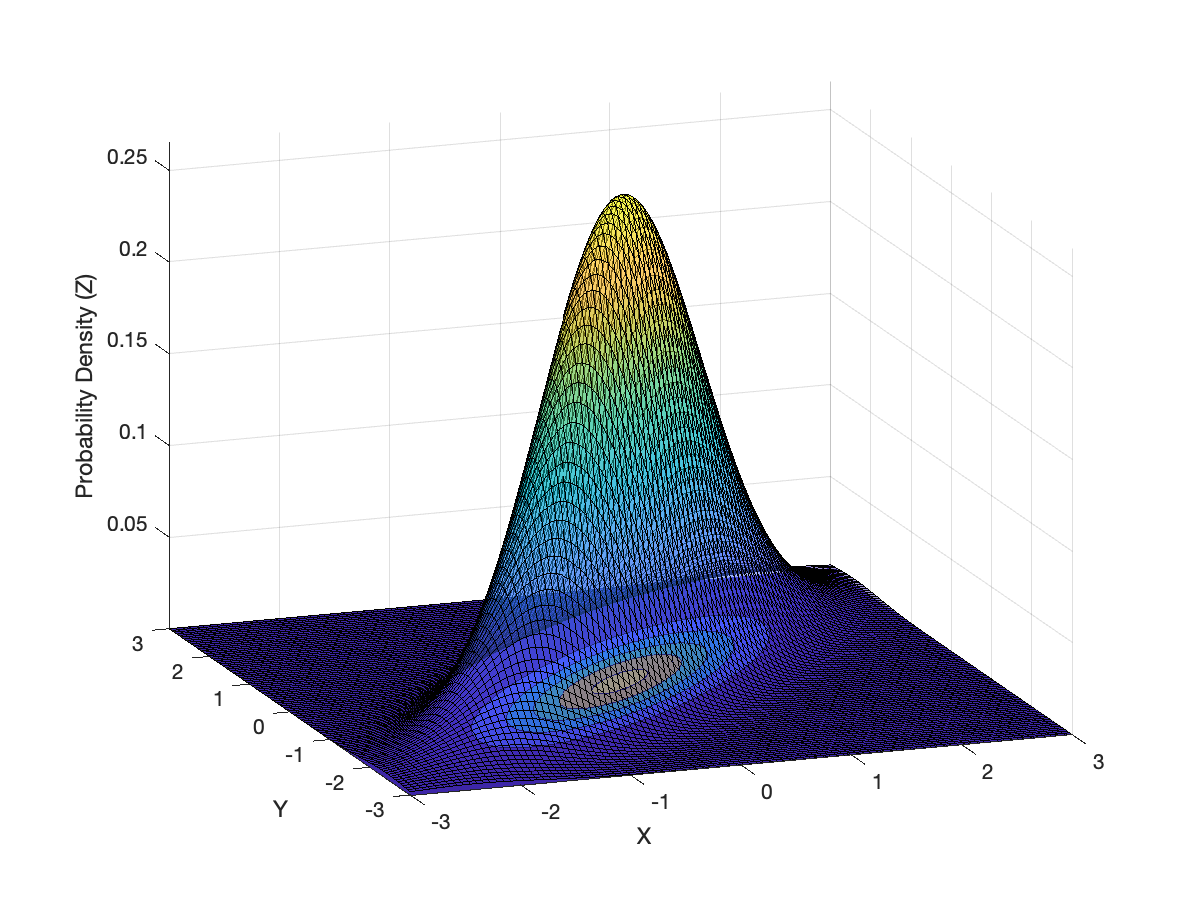
\includegraphics[width=0.75\textwidth]{Figures/Background2/GaussuanSurface_Corr_0.8.eps}
        \vspace{-10pt}
        \caption{Bivariate Gaussian distribution ($\rho=0.4$).}
    \end{figure}
        \column{0.5\textwidth}
            \begin{figure}
    \centering
    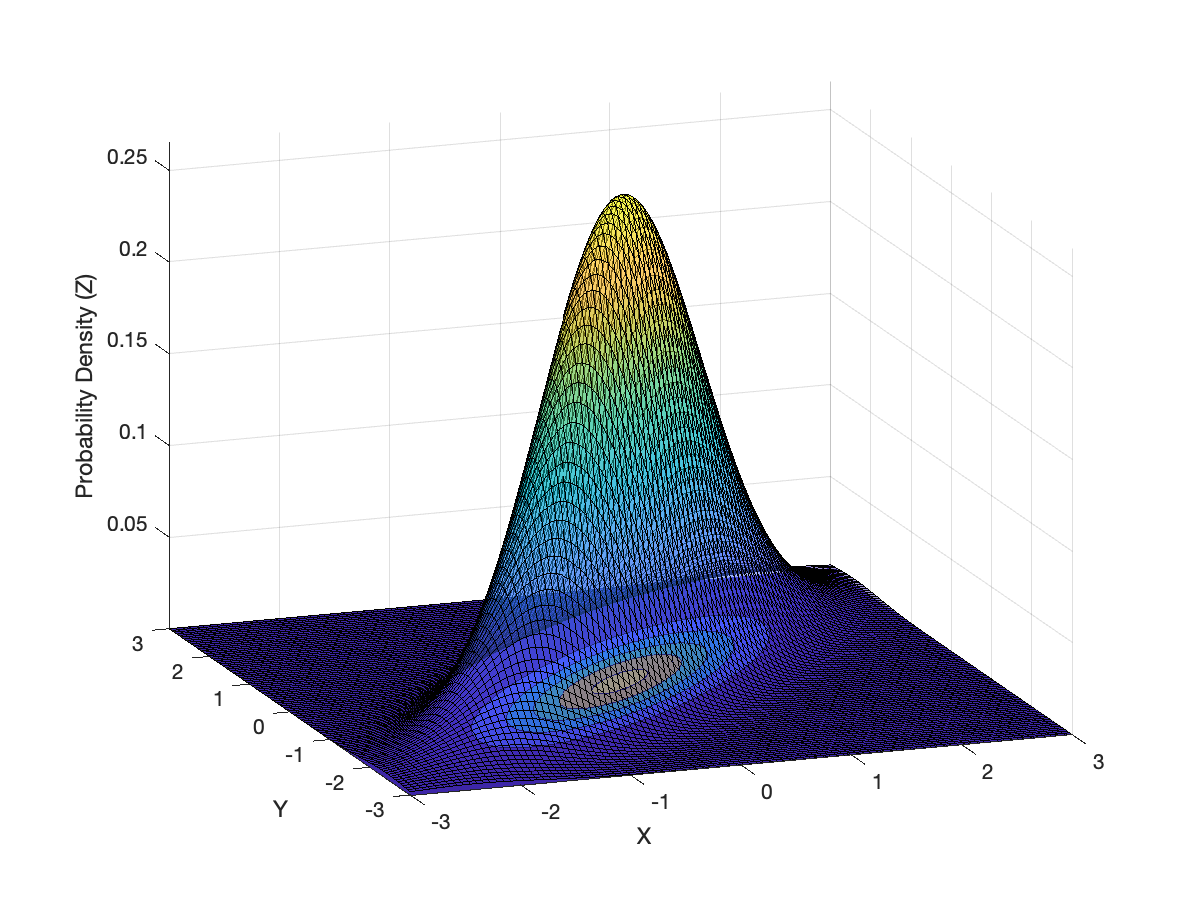
\includegraphics[width=0.75\textwidth]{Figures/Background2/GaussuanSurface_Corr_0.8.eps}
        \vspace{-10pt}
        \caption{Bivariate Gaussian distribution ($\rho=0.8$).}
    \end{figure}
\end{columns}



\end{frame}

%-------------------------------------------------------
\subsubsection{Bivariate Normal Distribution}
\begin{frame}{The Background Break - Bivariate Normal Distribution}
\begin{columns}
        \column{0.5\textwidth} 
For univariate distribution, the area between the $1\sigma$ boundaries is 68.26\% of the total area under the Gaussian function.
                \begin{figure}
            \centering
    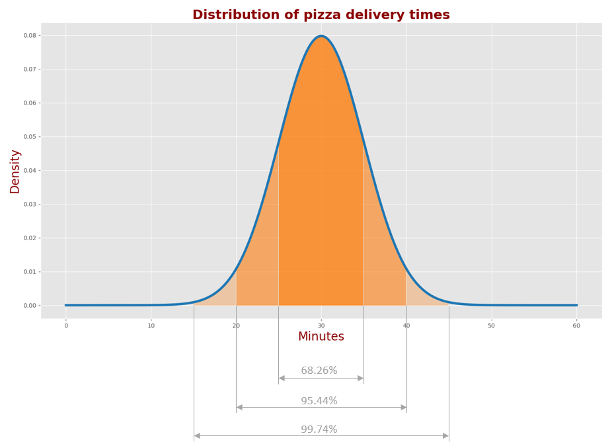
\includegraphics[width=1\textwidth]{Figures/Background2/UnivariateGaussian.png}
        \vspace{-10pt}
        \caption{Univariate Gaussian.}
    \end{figure}
        \column{0.5\textwidth}
        The probability of the bivariate normal distribution is a volume of the 3D
Gaussian function. For example, the volume of the 3D Gaussian function sliced at  $1\sigma$ 
level is 39.35\% of the total volume of the 3D Gaussian function.
        \begin{figure}
            \centering
    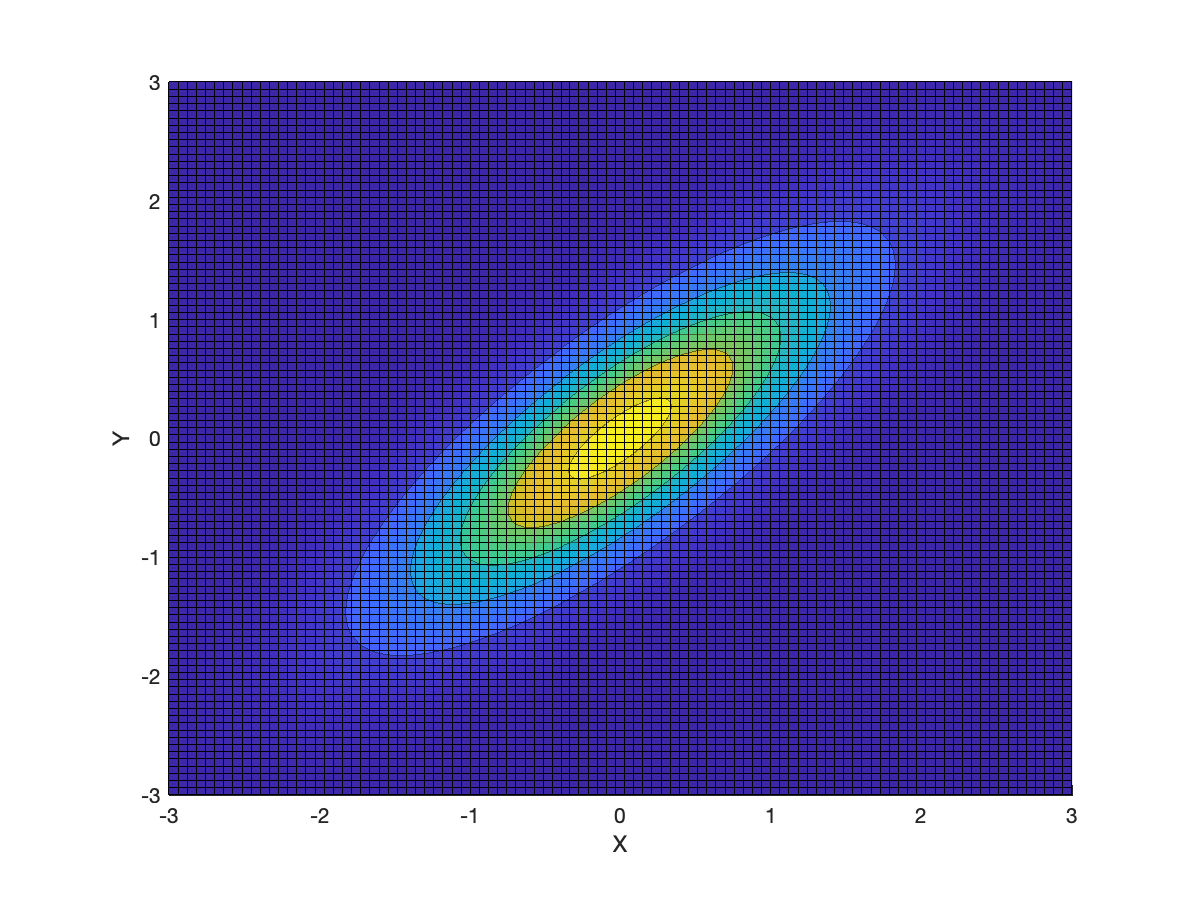
\includegraphics[width=1\textwidth]{Figures/Background2/GaussianContour_Corr_0.8.eps}
        \vspace{-10pt}
        \caption{Bivariate Gaussian distribution - Contour ($\rho=0.4$).}
    \end{figure}
    \texttt{\tiny [Code: Multivariate KF/bivariateGaussian\_withContours.m]}
\end{columns}
\end{frame}
%-------------------------------------------------------
\subsubsection{Covariance Ellipse}
\begin{frame}{The Background Break - Bivariate Normal Distribution - Covariance Ellipse}

\begin{itemize}
    \item The covariance ellipse represents an \textit{iso-contour} of the Gaussian distribution and allows visualization of a $1\sigma$ confidence interval in two dimensions. 
    \item It provides a geometric interpretation of the covariance matrix.
    \item Any ellipse can be described by four parameters:
    \begin{itemize}
        \item Ellipse center $\mu_x$, $\mu_y$
        \item Half-major axis $a$
        \item Half-minor axis $b$
        \item Orientation angle $\theta$
    \end{itemize}
    \begin{figure}
        \centering
        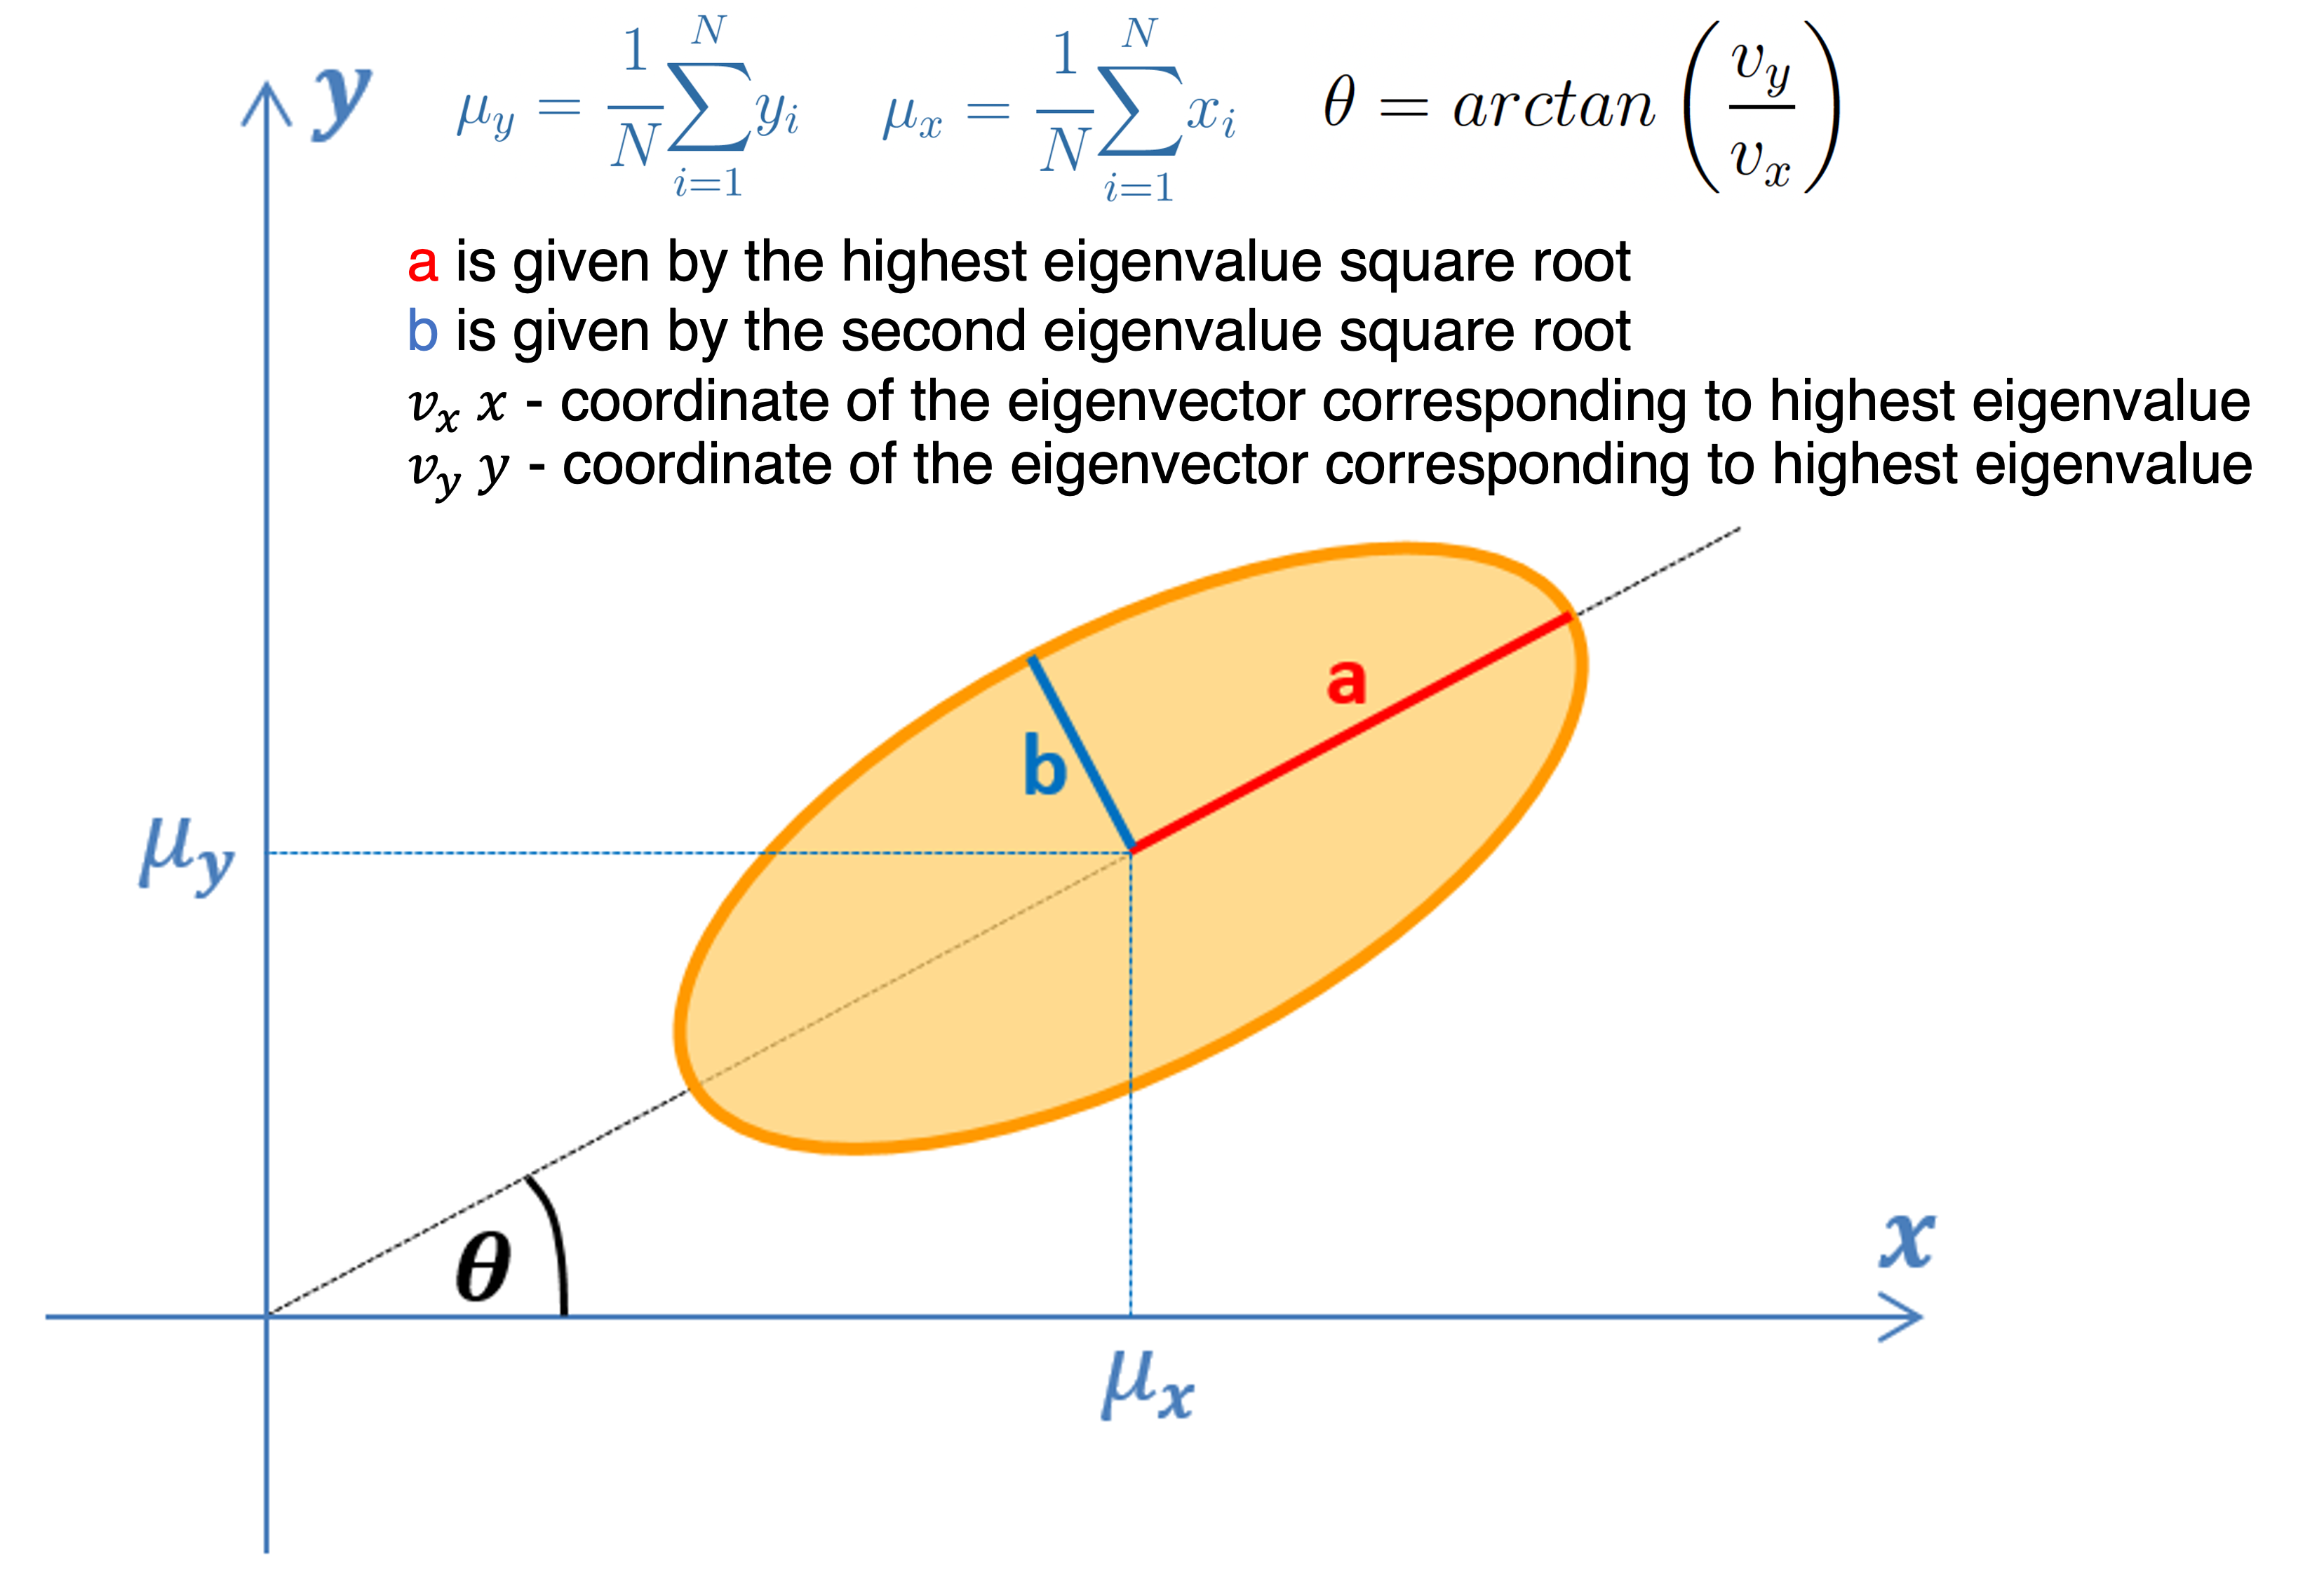
\includegraphics[width=0.6\textwidth]{Figures/Background2/CovarianceEllipse.png}
        \vspace{-10pt}
        \caption{Covariance ellipse.}
    \end{figure}
    

\end{itemize}

\end{frame}
%-------------------------------------------------------
\subsubsection{Confidence Ellipse}
\begin{frame}{The Background Break - Confidence Ellipse and Finding Probability Boundaries}

\begin{itemize}
    \item Often there is an interest in finding the boundaries of specific probability. For example, for 95\% probability, we should find the boundary that includes 95\% of Gaussian function volume.
    \item The projection of this boundary onto the \(x - y\) plane is the confidence ellipse. 
    \item \textbf{Find an elliptical scale factor \(k\), that extends the covariance ellipse to the confidence ellipse associated with 95\% probability.}
    \end{itemize}
    \begin{figure}
        \centering
        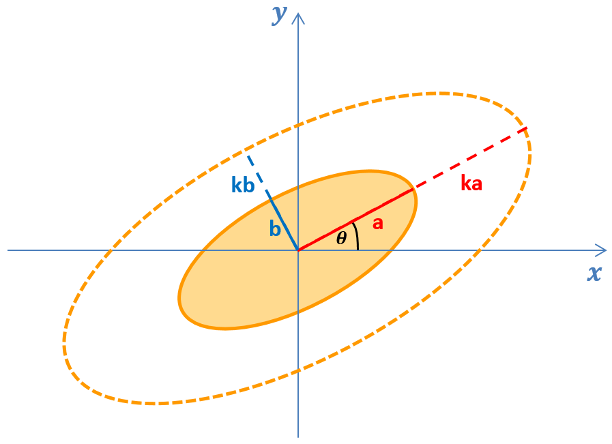
\includegraphics[width=0.6\textwidth]{Figures/Background2/ConfidenceEllipse.png}
        \vspace{-10pt}
        \caption{Covariance ellipse.}
    \end{figure}
\end{frame}
\begin{frame}{The Background Break - Confidence Ellipse and Finding Probability Boundaries}
   \begin{itemize} 
    \item As \(\sigma_x\) and \(\sigma_y\) represent the standard deviations of stochastically independent random variables, the addition theorem for the chi-square distribution may be used to show that the probability associated with a confidence ellipse is given by:
    $$p = 1 - \exp\left(-\frac{1}{2}k^2\right)$$
    \item For a covariance ellipse \(k = 1\), the probability associated with a covariance ellipse is:
    $$p = 1 - \exp\left(-\frac{1}{2}\right) = 39.35\%$$
    \item For a given probability, we can find an elliptical scale factor: $$k = \sqrt{-2\ln(1 - p)}$$
    \item For the probability of 95\%: $$k = \sqrt{-2\ln(1 - 0.95)} = 2.45$$
\end{itemize}

The properties of the confidence ellipse associated with 95\% probability are:
\begin{itemize}
    \item Ellipse center \((\mu_x, \mu_y)\) is similar to the covariance ellipse.
    \item Orientation angle \(\theta\) is similar to the covariance ellipse.
    \item Half-major axis length is \(2.45a\) – a scaled half-major axis of the covariance ellipse.
    \item Half-minor axis length is \(2.45b\) – a scaled half-minor axis of the covariance ellipse.
\end{itemize}
\end{frame}

%%%%%%%%%%%%%%%%%%%%%%%%%%%%%%%%%%%%%%%%%%%%%%%%%%%%%%%%%%%%%%%%%%%%%%%%%%%%%%%%%%%%%%%%%%%%%%%%%%%%%%%%%%%%%%%%%%%%%%%%%%%

\subsection{State Extrapolation Equation}
\begin{frame}{State Extrapolation Equation or Predictor Equation or Transition Equation or Dynamic Model or State Space Model}
Using the \textcolor{blue}{state extrapolation equation}, we can predict the \textbf{next system state} based
on the knowledge of the \textbf{current state}. \textcolor{blue}{It extrapolates the state vector from the
present (time step $n$) to the future (time step $n + 1$).}   

The State Extrapolation Equation can be expressed as:
\begin{minipage}{1\linewidth} % Adjust the width as needed
\begin{exampleblock}{}{
\begin{equation}
\mathbf{\hat{x}}_{n+1,n} = \mathbf{F} \mathbf{\hat{x}}_{n,n} + \mathbf{G} \mathbf{u}_{n} + \mathbf{w}_{n}\tag{1}
\end{equation}

where:
\begin{itemize}
    \item $\mathbf{\hat{x}}_{n+1,n}$ is a predicted system state vector at time step $n + 1$.
    \item $\mathbf{\hat{x}}_{n,n}$ is an estimated system state vector at time step $n$.
    \item $\mathbf{u}_{n}$ is a control variable or input variable - a measurable (deterministic) input to the system.
    \item $\mathbf{w}_{n}$ is a process noise or disturbance - an unmeasurable input that affects the state.
    \item $\mathbf{F}$ is a state transition matrix.
    \item $\mathbf{G}$ is a control matrix or input transition matrix (mapping control to state variables).
\end{itemize}}
\end{exampleblock}
\end{minipage}

\textit{*The process noise $w_n$ does not typically appear directly in the equations of
interest. Instead, this term is used to model the uncertainty in the Covariance
Extrapolation Equation.}
\end{frame}
%--------------------------------------------------

\begin{frame}{State Extrapolation Equation}
\begin{itemize}
    \item The state variables may represent attributes of the system that we wish to know. For example, a moving vehicle has three attributes: position, velocity, and acceleration.
\begin{figure}
    \centering
    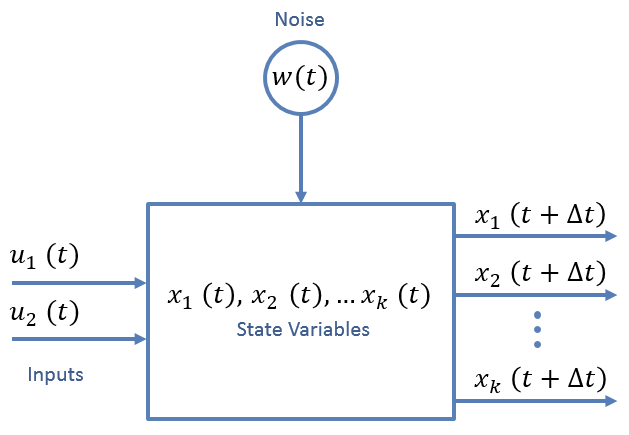
\includegraphics[width=0.5\linewidth]{Figures//Chapter2/KalmanFilterExtrapolation.png}
    \caption{Kalman Filter Extrapolation}
    \label{fig:KF_Extrapolation}
\end{figure}
\end{itemize}
\end{frame}
%---------------------------------------
\begin{frame}{State Extrapolation Equation}
Which attributes are the state variables, and which attributes are the input to the system?
\begin{itemize}
    \item Moving mechanical systems have attributes such as position, velocity, acceleration, and drag.
    \item A force that acts on a system should be considered an external forcing function, i.e., an input to the system that controls the state vector (position and velocity in the constant acceleration case).
    \item Newton’s second law tells us that $F = ma$. Thus we can consider acceleration as an external input to the system.
    \item The position and the velocity are the primary state variables of interest.
\end{itemize}

\begin{columns}
        \column{0.5\textwidth} 
        \textcolor{blue}{In a spring system, the force applied to the spring $F(t)$ is an input $u(t)$, while the spring displacement $x(t)$ is the system state.}
        \begin{figure}
            \centering
            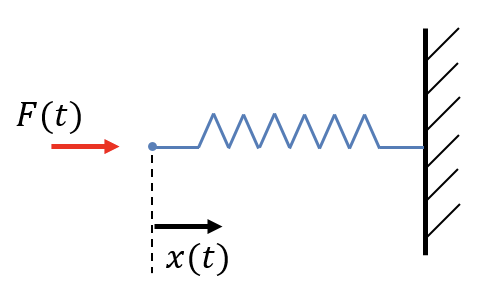
\includegraphics[width=0.7\textwidth]{Figures//Chapter2/SpringSystem.png}
            \caption{Spring System}
            \label{fig:SpringSystem}
        \end{figure}
        
        \column{0.5\textwidth}
        \textcolor{blue}{For a falling object, the inputs are the gravitational force $F_g$ and the drag force $F_{\text{drag}}(t)$, while the object height $h(t)$ and velocity $v(t)$ are the system states.}
        \begin{figure}
            \centering
            \includegraphics[width=0.3\textwidth]{Figures//Chapter2/FallingObject.png}
            \vspace{-10pt}
            \caption{Falling Object}
            \label{fig:FallingObject}
        \end{figure}
\end{columns}

\end{frame}    

%--------------------------------------------------
\subsection{Example - airplane - no control input}
\begin{frame}{State Extrapolation Equation (Example - airplane - no control input)}
Let's define the State Extrapolation Equation for an airplane moving in three-dimensional space with constant acceleration (i.e., there is no control input, $u_n = 0$).

The state vector $\mathbf{\hat{x}}_n$ ( describing the estimated airplane position, velocity, and acceleration in a cartesian coordinate system $(x, y, z)$), the state transition matrix $\mathbf{F}$ is:
\begin{columns}
        \column{0.2\textwidth} 
           \begin{equation*}
            \centering
            \mathbf{\hat{x}}_n =
            \begin{bmatrix}
            \hat{x}_n\\
            \hat{y}_n\\
            \hat{z}_n\\
            \hat{\dot{x}}_n\\
            \hat{\dot{y}}_n\\
            \hat{\dot{z}}_n\\
            \hat{\ddot{x}}_n\\
            \hat{\ddot{y}}_n\\
            \hat{\ddot{z}}_n\\
            \end{bmatrix}
            \end{equation*}
        \column{0.8\textwidth}
            $$\mathbf{F} =
\begin{bmatrix}
1 & 0 & 0 & \Delta t & 0 & 0 & 0.5\Delta t^2 & 0 & 0 \\
0 & 1 & 0 & 0 & \Delta t & 0 & 0 & 0.5\Delta t^2 & 0 \\
0 & 0 & 1 & 0 & 0 & \Delta t & 0 & 0 & 0.5\Delta t^2 \\
0 & 0 & 0 & 1 & 0 & 0 & \Delta t & 0 & 0 \\
0 & 0 & 0 & 0 & 1 & 0 & 0 & \Delta t & 0 \\
0 & 0 & 0 & 0 & 0 & 1 & 0 & 0 & \Delta t \\
0 & 0 & 0 & 0 & 0 & 0 & 1 & 0 & 0 \\
0 & 0 & 0 & 0 & 0 & 0 & 0 & 1 & 0 \\
0 & 0 & 0 & 0 & 0 & 0 & 0 & 0 & 1 \\
\end{bmatrix}$$ 
\end{columns}

$$\quad\quad\begin{bmatrix}
\hat{x}_{n+1,n} \\
\hat{y}_{n+1,n} \\
\hat{z}_{n+1,n} \\
\dot{\hat{x}}_{n+1,n} \\
\dot{\hat{y}}_{n+1,n} \\
\dot{\hat{z}}_{n+1,n} \\
\ddot{\hat{x}}_{n+1,n} \\
\ddot{\hat{y}}_{n+1,n} \\
\ddot{\hat{z}}_{n+1,n}
\end{bmatrix}
=
\begin{bmatrix}
1 & 0 & 0 & \Delta t & 0 & 0 & 0.5\Delta t^2 & 0 & 0 \\
0 & 1 & 0 & 0 & \Delta t & 0 & 0 & 0.5\Delta t^2 & 0 \\
0 & 0 & 1 & 0 & 0 & \Delta t & 0 & 0 & 0.5\Delta t^2 \\
0 & 0 & 0 & 1 & 0 & 0 & \Delta t & 0 & 0 \\
0 & 0 & 0 & 0 & 1 & 0 & 0 & \Delta t & 0 \\
0 & 0 & 0 & 0 & 0 & 1 & 0 & 0 & \Delta t \\
0 & 0 & 0 & 0 & 0 & 0 & 1 & 0 & 0 \\
0 & 0 & 0 & 0 & 0 & 0 & 0 & 1 & 0 \\
0 & 0 & 0 & 0 & 0 & 0 & 0 & 0 & 1
\end{bmatrix}
\begin{bmatrix}
\hat{x}_{n,n} \\
\hat{y}_{n,n} \\
\hat{z}_{n,n} \\
\dot{\hat{x}}_{n,n} \\
\dot{\hat{y}}_{n,n} \\
\dot{\hat{z}}_{n,n} \\
\ddot{\hat{x}}_{n,n} \\
\ddot{\hat{y}}_{n,n} \\
\ddot{\hat{z}}_{n,n}
\end{bmatrix}$$

       
\end{frame}
%--------------------------------------------------
\begin{frame}{State Extrapolation Equation (Example - airplane - no control input)}
The state update equations after matrix multiplication are given by:
\begin{align*}
\hat{x}_{n+1,n} &= \hat{x}_{n,n} + \hat{\dot{x}}_{n,n}\Delta t + \frac{1}{2}\hat{\ddot{x}}_{n,n}\Delta t^2 \\
\hat{y}_{n+1,n} &= \hat{y}_{n,n} + \hat{\dot{y}}_{n,n}\Delta t + \frac{1}{2}\hat{\ddot{y}}_{n,n}\Delta t^2 \\
\hat{z}_{n+1,n} &= \hat{z}_{n,n} + \hat{\dot{z}}_{n,n}\Delta t + \frac{1}{2}\hat{\ddot{z}}_{n,n}\Delta t^2 \\
\hat{\dot{x}}_{n+1,n} &= \hat{\dot{x}}_{n,n} + \hat{\ddot{x}}_{n,n}\Delta t \\
\hat{\dot{y}}_{n+1,n} &= \hat{\dot{y}}_{n,n} + \hat{\ddot{y}}_{n,n}\Delta t \\
\hat{\dot{z}}_{n+1,n} &= \hat{\dot{z}}_{n,n} + \hat{\ddot{z}}_{n,n}\Delta t \\
\hat{\ddot{x}}_{n+1,n} &= \hat{\ddot{x}}_{n,n} \\
\hat{\ddot{y}}_{n+1,n} &= \hat{\ddot{y}}_{n,n} \\
\hat{\ddot{z}}_{n+1,n} &= \hat{\ddot{z}}_{n,n}
\end{align*}
\end{frame}

%------------------------------------------------
\subsection{Example - airplane - with control input}
\begin{frame}{State Extrapolation Equation (Example - airplane - with control input)}

Considering additional information about the airplane
acceleration (based on the pilot’s controls) based on the pilot’s commands.

\begin{columns}
        \column{0.5\textwidth}
        The state vector $\mathbf{\hat{x}}_n$ ( describing the estimated airplane position and velocity a cartesian coordinate system $(x, y, z)$) is:
           \begin{equation*}
            \centering
            \mathbf{\hat{x}}_n =
            \begin{bmatrix}
            \hat{x}_n\\
            \hat{y}_n\\
            \hat{z}_n\\
            \hat{\dot{x}}_n\\
            \hat{\dot{y}}_n\\
            \hat{\dot{z}}_n\\
            \end{bmatrix}
            \end{equation*}
        The control vector $u_n$ that describes the measured airplane acceleration in a cartesian coordinate system $(x, y, z)$ is:
        \begin{equation*}
            \centering
            \mathbf{{u}}_n =
            \begin{bmatrix}
            \hat{\ddot{x}}_n\\
            \hat{\ddot{y}}_n\\
            \hat{\ddot{z}}_n\\
            \end{bmatrix}
        \end{equation*} 
        \column{0.5\textwidth}
        The state transition matrix $\mathbf{F}$ is:
        $$\mathbf{F} = \begin{bmatrix}
        1 & 0 & 0 & \Delta t & 0 & 0 \\
        0 & 1 & 0 & 0 & \Delta t & 0 \\
        0 & 0 & 1 & 0 & 0 & \Delta t\\
        0 & 0 & 0 & 1 & 0 & 0 \\
        0 & 0 & 0 & 0 & 1 & 0 \\
        0 & 0 & 0 & 0 & 0 & 1 \\
        \end{bmatrix}$$ 
        The control matrix $\mathbf{G}$ is:
        $$\mathbf{G} = \begin{bmatrix}
        0.5\Delta t^2 & 0 & 0 \\
        0 & 0.5\Delta t^2 & 0 \\
        0 & 0 & 0.5\Delta t^2 \\
        \Delta t & 0 & 0 \\
        0 & \Delta t & 0 \\
        0 & 0 & \Delta t \\
        \end{bmatrix}$$
        \end{columns}

\end{frame}
%-----------------------------------------------
%------------------------------------------------
\begin{frame}{State Extrapolation Equation (Example - airplane - with control input)}

The state extrapolation equation is:
$$\hat{x}_{n+1,n} = \mathbf{F}\hat{x}_{n,n} + \mathbf{G}u_{n,n}$$

Given the system dynamics, the state update can be expressed as:
\begin{equation}
\left[
\begin{array}{c}
\hat{x}_{n+1,n} \\
\hat{y}_{n+1,n} \\
\hat{z}_{n+1,n} \\
\dot{\hat{x}}_{n+1,n} \\
\dot{\hat{y}}_{n+1,n} \\
\dot{\hat{z}}_{n+1,n} \\
\end{array}
\right]
\!=\!
\left[
\begin{array}{cccccc}
1 & 0 & 0 & \Delta t & 0 & 0 \\
0 & 1 & 0 & 0 & \Delta t & 0 \\
0 & 0 & 1 & 0 & 0 & \Delta t \\
0 & 0 & 0 & 1 & 0 & 0 \\
0 & 0 & 0 & 0 & 1 & 0 \\
0 & 0 & 0 & 0 & 0 & 1 \\
\end{array}
\right]
\left[
\begin{array}{c}
\hat{x}_{n,n} \\
\hat{y}_{n,n} \\
\hat{z}_{n,n} \\
\dot{\hat{x}}_{n,n} \\
\dot{\hat{y}}_{n,n} \\
\dot{\hat{z}}_{n,n} \\
\end{array}
\right]
\!+\!
\left[
\begin{array}{ccc}
0.5\Delta t^2 & 0 & 0 \\
0 & 0.5\Delta t^2 & 0 \\
0 & 0 & 0.5\Delta t^2 \\
\Delta t & 0 & 0 \\
0 & \Delta t & 0 \\
0 & 0 & \Delta t \\
\end{array}
\right]
\left[
\begin{array}{c}
\ddot{x}_n \\
\ddot{y}_n \\
\ddot{z}_n \\
\end{array}
\right]\nonumber
\end{equation}

\end{frame}
%---------------------------------------------
\subsection{Example – Falling Object}
\begin{frame}{State Extrapolation Equation (Example – Falling Object)}

Consider a free-falling object. The state vector includes the altitude \(h\) and the object's velocity \(\dot{h}\):
\begin{equation}
\hat{\mathbf{x}}_n = 
\begin{bmatrix}
\hat{h}_n \\
\dot{\hat{h}}_n
\end{bmatrix}
\end{equation}

The state transition matrix \(\mathbf{F}\) is:
\begin{equation}
\mathbf{F} = 
\begin{bmatrix}
1 & \Delta t \\
0 & 1
\end{bmatrix}
\end{equation}

The control matrix \(\mathbf{G}\) is:
\begin{equation}
\mathbf{G} = 
\begin{bmatrix}
0.5\Delta t^2 \\
\Delta t
\end{bmatrix}
\end{equation}

The input variable \(u_n\) is:
\begin{equation}
u_n = 
\begin{bmatrix}
g 
\end{bmatrix}
[\text{the gravitational acceleration}]
\end{equation}

We don’t have a sensor that measures acceleration, but we know that for a falling object, acceleration equals \(g\).

The state extrapolation equation is:
\begin{equation}
\begin{bmatrix}
\hat{h}_{n+1,n} \\
\dot{\hat{h}}_{n+1,n}
\end{bmatrix}
=
\begin{bmatrix}
1 & \Delta t \\
0 & 1
\end{bmatrix}
\begin{bmatrix}
\hat{h}_{n,n} \\
\dot{\hat{h}}_{n,n}
\end{bmatrix}
+
\begin{bmatrix}
0.5\Delta t^2 \\
\Delta t
\end{bmatrix}
\begin{bmatrix}
g
\end{bmatrix}
\end{equation}

The matrix multiplication results in the following:
\begin{align}
\hat{h}_{n+1,n} &= \hat{h}_{n,n} + \dot{\hat{h}}_{n,n}\Delta t + 0.5\Delta t^2g \notag \\
\dot{\hat{h}}_{n+1,n} &= \dot{\hat{h}}_{n,n} + \Delta tg \notag
\end{align}

\end{frame}
%------
\begin{frame}{Linear Time-Invariant Systems}
The Linear Kalman Filter assumes the Linear Time-Invariant (LTI) system model.

\textbf{So, what is “linear,” and what is “time-invariant”?}

\begin{block}{Linear Systems}
Linear systems are described by systems of equations in which the variables are never multiplied with each other but only with constants and then summed up. They are used to describe both static and dynamic relationships between variables.

A linear system is a system whose output function \(y(t)\) satisfies the following equation:
\[y(t) = F (a \times g(t) + b \times h(t)) = a \times F(g(t)) + b \times F(h(t))\]
\begin{itemize}
    \item \(a\) and \(b\) are constant real numbers.
    \item \(g\) and \(h\) are any arbitrary functions of an independent variable \(t\).
\end{itemize}

A linear system follows two basic rules:
\begin{enumerate}
    \item You can “factor out” constant multiplicative scale factors.
    \item The system’s response to a sum of inputs is the sum of the responses to each input separately.
\end{enumerate}
\end{block}
\end{frame}

\begin{frame}{Linear Time-Invariant Systems}
    
\begin{block}{Time-Invariant Systems}
A time-invariant system has a system function that is not a direct function of time. For example, an amplifier with gain \(G = 10\). This system is time-invariant. Although the system’s output changes with time, the system function is not time-dependent.

\begin{figure}
    \centering
    \includegraphics[width=0.6\linewidth]{Figures//Chapter2/Amplifier.png}
    \caption{Amplifier}
    \vspace{-10pt}
    \label{fig:amplifier}
\end{figure}

A time-invariant system is one where a time delay (or shift) in the input sequence causes an equivalent time delay in the system’s output sequence.
\end{block}

\textbf{See Appendix~C of the book "Kalman Filter from the ground up" by Alex Becker for generalized dynamic model derivation for any linear dynamic model.}

\end{frame}

%%%%%%%%%%%%%%%%%%%%%%%%%%%%%%%%%%%%%%%%%

\subsection{Covariance Extrapolation Equation}
\begin{frame}{Covariance Extrapolation Equation}
The general form of the Covariance Extrapolation Equation is given by:
\begin{minipage}{1\linewidth} % Adjust the width as needed
\begin{exampleblock}{}{
\begin{equation*}
\mathbf{P}_{n+1,n} = \mathbf{F}\mathbf{P}_{n,n}\mathbf{F}^T + \mathbf{Q} \tag{2}
\end{equation*}

where:
\begin{itemize}
    \item $\mathbf{P}_{n,n}$ is the squared uncertainty of an estimate (covariance matrix) of the current state.
    \item $\mathbf{P}_{n+1,n}$ is the squared uncertainty of a prediction (covariance matrix) for the next state.
    \item $\mathbf{F}$ is the state transition matrix that we derived in Appendix C (“Modeling linear dynamic systems”).
    \item $\mathbf{Q}$ is the process noise matrix.
\end{itemize}}
\end{exampleblock}
\end{minipage}

\end{frame}
%---------------------------------------------------
\subsubsection{The estimate covariance without process noise}
\begin{frame}{The estimate covariance without process noise}
Assuming $\mathbf{Q}=0$:
$\mathbf{P}_{n+1,n}=\mathbf{F}\mathbf{P}_{n,n}\mathbf{F}^T$

The covariance of a vector \(\mathbf{x}\) is defined as:
\begin{equation*}
{COV}(\mathbf{x}) = \mathbb{E}\left[ (\mathbf{x}-\boldsymbol{\mu}_{\mathbf{x}})(\mathbf{x}-\boldsymbol{\mu}_{\mathbf{x}})^T \right] (\text{vector}~\mathbf{x}~\text{is a system state vector})
\end{equation*}

Therefore, the covariance matrix \(\mathbf{P}_{n,n}\) is:
\begin{equation*}
\mathbf{P}_{n,n} = \mathbb{E}\left[ (\hat{\mathbf{x}}_{n,n} - \boldsymbol{\mu}_{\mathbf{x}_{n,n}})(\hat{\mathbf{x}}_{n,n} - \boldsymbol{\mu}_{\mathbf{x}_{n,n}})^T \right]
\end{equation*}

For the next state, this becomes:
\begin{equation*}
\mathbf{P}_{n+1,n} = \mathbb{E}\left[ (\hat{\mathbf{x}}_{n+1,n} - \boldsymbol{\mu}_{\mathbf{x}_{n+1,n}})(\hat{\mathbf{x}}_{n+1,n} - \boldsymbol{\mu}_{\mathbf{x}_{n+1,n}})^T \right]
\end{equation*}

Following the state extrapolation equation:
\begin{equation*}
\hat{\mathbf{x}}_{n+1,n} = \mathbf{F} \hat{\mathbf{x}}_{n,n} + \mathbf{G}\hat{\mathbf{u}}_{n,n}
\end{equation*}

The update for the covariance matrix can be represented as:
\begin{align*}
\mathbf{P}_{n+1,n} & = \mathbb{E} \left[ (\mathbf{F} \mathbf{\hat{x}}_{n,n} + \mathbf{G}\mathbf{\hat{u}}_{n,n} - \mathbf{F}\mathbf{\mu}_{x,n,n} - \mathbf{G}\mathbf{\hat{u}}_{n,n}) \times (\mathbf{F} \mathbf{\hat{x}}_{n,n} + \mathbf{G}\mathbf{\hat{u}}_{n,n} - \mathbf{F}\mathbf{\mu}_{x,n,n} - \mathbf{G}\mathbf{\hat{u}}_{n,n})^T \right]\\
& = \mathbb{E} \left[ (\mathbf{F} (\mathbf{\hat{x}}_{n,n} - \mathbf{\mu}_{x,n}) ) (\mathbf{F} (\mathbf{\hat{x}}_{n,n} - \mathbf{\mu}_{x,n}) )^T \right]\\
& = \mathbb{E} \left[ (\mathbf{F} (\mathbf{\hat{x}}_{n,n} - \mathbf{\mu}_{x,n}) ) (\mathbf{\hat{x}}_{n,n} - \mathbf{\mu}_{x,n})^T \mathbf{F}^T\right] \quad ((\mathbf{AB})^T = \mathbf{B}^T\mathbf{A}^T)\\
& = \mathbf{F} \mathbb{E} \left[ ( (\mathbf{\hat{x}}_{n,n} - \mathbf{\mu}_{x,n}) ) (\mathbf{\hat{x}}_{n,n} - \mathbf{\mu}_{x,n})^T \right]\mathbf{F}^T \\
&= \mathbf{F}\mathbf{P}_{n,n}\mathbf{F}^T
\end{align*}

\end{frame}
%------------------------------------------
\subsubsection{Constructing the process noise matrix}
\begin{frame}{Constructing the process noise matrix $\mathbf{Q}$}
The system dynamics is described by:
\begin{equation*}
\mathbf{\hat{x}}_{n+1,n} = \mathbf{F}\mathbf{\hat{x}}_{n,n} + \mathbf{G}\mathbf{\hat{u}}_{n,n} + \underset{\text{Process noice}}{\mathbf{w}_n}
\end{equation*}     

In 1D Kalman Filter, the process noise variance is denoted by \textbf{q} while for 3D case by $\mathbf{Q}$. 

The process noise variance has a critical influence on the Kalman
Filter performance. 
\begin{itemize}
    \item Too small $q$ causes a lag error (Example 7).
    \item If the $q$ value is too high, the Kalman Filter follows the measurements (Example 8) and produces noisy estimations.
\end{itemize}

The process noise can be independent between different state variables. In this case, the process noise covariance matrix \( \mathbf{Q} \) is a diagonal matrix:
\begin{equation}
\mathbf{Q} = 
\begin{bmatrix}
q_{11} & 0 & \cdots & 0 \\
0 & q_{22} & \cdots & 0 \\
\vdots & \vdots & \ddots & \vdots \\
0 & 0 & \cdots & q_{kk}
\end{bmatrix}
\tag{8.32}
\end{equation}

The process noise can also be dependent. For example, the constant velocity model assumes zero acceleration (\(a = 0\)). However, a random variance in acceleration (\(\sigma^2_a\)) causes a variance in velocity and position. In this case, the process noise is correlated with the state variables.
\end{frame}


%------------------------------------------
\subsubsection{Discrete Noise Model}
\begin{frame}{Models for the environmental process noise - Discrete Noise}
\begin{columns}
        \column{0.5\textwidth} 
    \textcolor{blue}{There are two models for the environmental process noise; Discrete and Continuous noise model.}
    \begin{figure}
        \centering
        \includegraphics[width=0.6\linewidth]{Figures//Chapter2/DiscreteNoise.png}
        \vspace{-10pt}
        \caption{Discrete Noise}
        \vspace{-10pt}
        \label{fig:DiscreteNoise}
    \end{figure}
    The process noise covariance matrix \(\mathbf{Q}\) for the constant velocity model can be expressed as:
\begin{equation*}
\mathbf{Q} = 
\begin{bmatrix}
V(x) & \text{COV}(x, v) \\
\text{COV}(v, x) & V(v)
\end{bmatrix}
\end{equation*}
where \(V(x)\) and \(V(v)\) represent the position and velocity variance, respectively, and COV(x, v) is the covariance between position and velocity. These terms are expressed in terms of the random acceleration variance \(\sigma_a^2\) of the model.

        \column{0.5\textwidth}
\begin{align*}
V(v) &= \sigma_v^2 = E(v^2) - \mu_v^2\\
 & = E\left((a\Delta t)^2\right) - (\mu_a \Delta t)^2\\
& = \Delta t^2 \left( E(a^2) - \mu_a^2 \right)\\ & = \Delta t^2 \sigma_a^2\\
V(x) &= \sigma_x^2 = E(x^2) - \mu_x^2\\
& = E\left(\left(\frac{1}{2} a \Delta t^2\right)^2\right) - \left(\frac{1}{2} \mu_a \Delta t^2\right)^2\\
& = E\left((a\Delta t)^2\right) - (\mu_a \Delta t)^2\\
& = \Delta t^4 \left( \frac{1}{4} \right) \left( E(a^2) - \mu_a^2 \right)\\ 
& = \Delta t^4 \left( \frac{1}{4} \right) \sigma_a^2\\
\text{COV}(x, v) & = \text{COV}(v, x) = E(xv) - \mu_x\mu_v\\
& = \!\left( E\left( \frac{1}{2} a\Delta t^2 a\Delta t \right) \!-\! \left( \frac{1}{2} \mu_a\Delta t^2 \mu_a\Delta t \right)\! \right)\\ 
& = \frac{\Delta t^3}{2} \left( E(a^2) - \mu_a^2 \right) = \frac{\Delta t^3}{2} \sigma_a^2
\end{align*}
\end{columns}
\end{frame}
%----------------------------------------
\begin{frame}{Discrete Noise-How to construct  $\mathbf{Q}$ matrix}

By substituting the results into $\mathbf{Q}$ matrix:

    $$\mathbf{Q} = \sigma_a^2
\begin{bmatrix}
\frac{\Delta t^4}{4} & \frac{\Delta t^3}{2} \\
\frac{\Delta t^3}{2} & \Delta t^2 \\
\end{bmatrix}$$

There are two methods for a faster construction of the Q matrix
\begin{itemize}
    \item Projection using the state transition matrix (without control input)
    \item Projection using the control matrix (with control input)
\end{itemize}
\end{frame}

%------------------------------------------------
\begin{frame}{Discrete Noise: How to construct  $\mathbf{Q}$ matrix}
\label{DiscreteNoise_ConstructQMatrix}
\begin{columns}
        \column{0.5\textwidth} 
    \textbf{Without Control Input:}
    If the dynamic model doesn’t include a control input,  project the random variance in acceleration $\sigma_a^2$ on the dynamic model using state transition matrix $\mathbf{F}$.
    \begin{itemize}
        \item Let us define a matrix $\mathbf{Q}_a$:
        \[ \mathbf{Q}_a = \begin{bmatrix} 0 & 0 & 0 \\ 0 & 0 & 0 \\ 0 & 0 & 1 \end{bmatrix} \sigma_a^2 \]
        \item The process noise matrix is $\mathbf{Q} = \mathbf{F}\mathbf{Q}_a\mathbf{F}^T$.
        \item For the motion model, $\mathbf{F}$ matrix is:
        \vspace{-10pt}
        \[ \mathbf{F} = \begin{bmatrix} 1 & \Delta t  & \frac{\Delta t^2} {2}\\ 0 & 1 & \Delta t \\ 0 & 0 & 1 \end{bmatrix} \]
    \end{itemize}
    \vspace{-10pt}
    \begin{align*}
    Q \!& =\! \sigma_a^2 \!
    \begin{bmatrix}
    1 & \Delta t & \frac{\Delta t^2}{2} \\
    0 & 1 & \Delta t \\
    0 & 0 & 1 \\
    \end{bmatrix}\!\!\!
    \begin{bmatrix}
    0 & 0 & 0 \\
    0 & 0 & 0 \\
    0 & 0 & 1 \\
    \end{bmatrix}\!\!\!
    \begin{bmatrix}
    1 & 0 & 0 \\
    \Delta t & 1 & 0 \\
    \frac{\Delta t^2}{2} & \Delta t & 1 \\
    \end{bmatrix}\\
    & = \begin{bmatrix}
    \frac{\Delta t^4}{4} & \frac{\Delta t^3}{2} & \frac{\Delta t^2}{2} \\
    \frac{\Delta t^3}{2} & \Delta t^2 & \Delta t \\
    \frac{\Delta t^2}{2} & \Delta t & 1
    \end{bmatrix}
    \end{align*}
        \column{0.5\textwidth}
        \textbf{With Control Input:}
        When the dynamic model includes a control input, we can compute $\mathbf{Q}$ matrix even faster by projecting the random variance in acceleration $\sigma_a^2$ using the control matrix $\mathbf{G}$.

    \begin{itemize}
        \item $\mathbf{Q} = \mathbf{G}\sigma_a^2\mathbf{G}^T$ where $\mathbf{G}$ is the control (or input transition) matrix.
        \item For the motion model, the $\mathbf{G}$ matrix is:
        \[ \mathbf{G} = \begin{bmatrix} \frac{\Delta t^2}{2} \\ \Delta t \end{bmatrix} \]
    \end{itemize}

    \textbf{Resulting $\mathbf{Q}$ matrix:}
    \begin{align*}
        \mathbf{Q} & = \sigma_a^2 \mathbf{G} \mathbf{G}^T\\
        & = \sigma_a^2 \begin{bmatrix} \frac{\Delta t^2}{2} \\ \Delta t \end{bmatrix}\begin{bmatrix} \frac{\Delta t^2}{2} & \Delta t \end{bmatrix}\\
        & = \sigma_a^2 \begin{bmatrix} \frac{\Delta t^4}{4} & \frac{\Delta t^3}{2} \\ \frac{\Delta t^3}{2} & \Delta t^2 \end{bmatrix}
    \end{align*}
\end{columns}
\end{frame}
%---------------------------------------------
\begin{frame}{Continuous Noise: How to construct  $\mathbf{Q}$ matrix }
The continuous model assumes that the noise changes continuously over time.
    \begin{figure}
        \centering
        \includegraphics[width=0.4\linewidth]{Figures//Chapter2/ContinuousNoise.png}
        \caption{Continuous Noise}
        \label{fig:ContinuousNoise}
    \end{figure}


To derive the process noise covariance matrix for the continuous model $\mathbf{Q}_c$, we need to integrate the discrete process noise covariance matrix $\mathbf{Q}$ over time.

\[
\mathbf{Q}_{c} = \int_{0}^{\Delta t} \mathbf{Q} dt = \int_{0}^{\Delta t} \sigma_a^2 
\begin{bmatrix}
\frac{t^4}{4} & \frac{t^3}{2} \\
\frac{t^3}{2} & t^2
\end{bmatrix}
dt = \sigma_a^2 
\begin{bmatrix}
\frac{\Delta t^5}{20} & \frac{\Delta t^4}{8} \\
\frac{\Delta t^4}{8} & \frac{\Delta t^3}{3}
\end{bmatrix}
\]
\end{frame}
%---------------------------------------------
\begin{frame}{Selecting Process Noise Variance and Noise Model} 
\begin{block}{Process Noise Variance ($\sigma_a^2$)}
\begin{itemize}
    \item Calculated using stochastic statistics or chosen based on engineering practice.
    \item Depends on target characteristics and model completeness.
    \item For \textbf{maneuvering targets} (e.g., airplanes), $\sigma_a^2$ should be relatively high.
    \item For \textbf{non-maneuvering targets} (e.g., rockets), a smaller $\sigma_a^2$ is appropriate.
    \item Environmental influences like air drag reduce process noise randomness if included in the model.
\end{itemize}
\end{block}

\begin{block}{Choosing the Noise Model}
\begin{itemize}
    \item No definitive answer: recommend trying both discrete and continuous models.
    \item Use \textbf{discrete noise model} when $\Delta t$ is small.
    \item Prefer \textbf{continuous noise model} when $\Delta t$ is high.
    \item Experiment to see which model performs better with your Kalman Filter.
\end{itemize}
\end{block}
\end{frame}

%-------------------------------------------------------
\subsection{Auxiliary Equations}
\subsubsection{Measurement Equation}
\begin{frame}{Measurement Equation}
In 1D KF, measurement denoted by $z_n$
\begin{itemize}
    \item Represented the true system state plus random measurement noise $v_n$.
\end{itemize}

Measurement Noise Variance ($r_n$):
\begin{itemize}
    \item Can be \textbf{constant} for all measurements (e.g., scales with a precision of 0.5 kg).
    \item May \textbf{vary} for each measurement (e.g., thermometer with 0.5\% precision).
    \item In variable cases, the noise variance depends on the measured quantity (e.g., temperature).
\end{itemize}

\begin{minipage}{1\linewidth} 
\begin{exampleblock}{}{
The Measurement Equation is given by:
\begin{equation*}
\mathbf{z}_n = \mathbf{H}\mathbf{x}_n + \mathbf{v}_n
\end{equation*}

where:
\begin{itemize}
    \item $\mathbf{z}_n$ is a measurement vector.
    \item $\mathbf{x}_n$ is a true system state (hidden state).
    \item $\mathbf{v}_n$ is a random noise vector.
    \item $\mathbf{H}$ is an observation matrix.
\end{itemize}}
\end{exampleblock}
\end{minipage}

\end{frame}
%------------------------------------------------------------
\begin{frame}{The Observation Matrix}

In many scenarios, the measured value is not the direct system state we are interested in. For instance, a digital electric thermometer measures an electric current, which needs to be translated to temperature -- the actual system state of interest.

\vspace{5pt}
The observation matrix $\mathbf{H}$ serves the crucial function of transforming the system state (input) into the measurement (output) through linear transformations. This process ensures that the Kalman Filter can work with measurements that represent the system states accurately.

\vspace{5pt}
\textbf{Scaling:} A range meter sends a signal toward a destination and receives a reflected echo. The
measurement is the time delay between the transmission and reception of the signal. The system state is the range.

In this case, we need to perform a scaling:
\begin{equation*}
z_n = \begin{bmatrix} \frac{2}{c} \end{bmatrix} x_n + v_n
\end{equation*}
\begin{equation*}
H = \begin{bmatrix} \frac{2}{c} \end{bmatrix}
\end{equation*}

where:
\begin{itemize}
    \item \(c\) is the speed of light.
    \item \(x_n\) is the range.
    \item \(z_n\) is the measured time delay.
\end{itemize}

\end{frame}
%------------------------------------------------------------
\begin{frame}{The Observation Matrix}
\textbf{State selection:} Sometimes certain states are measured while others are not. For example, the first,
third, and fifth states of a 5D state vector are measurable, while the second and fourth states are not measurable:
$$z_n = \mathbf{H}\mathbf{x}_n + \mathbf{v}_n = 
\begin{bmatrix}
1 & 0 & 0 & 0 & 0 \\
0 & 0 & 1 & 0 & 0 \\
0 & 0 & 0 & 0 & 1 \\
\end{bmatrix}
\begin{bmatrix}
x_1 \\
x_2 \\
x_3 \\
x_4 \\
x_5 \\
\end{bmatrix}
+ \mathbf{v}_n = 
\begin{bmatrix}
x_1 \\
x_3 \\
x_5 \\
\end{bmatrix}
+ \mathbf{v}_n$$

\textbf{Combination of states:} Sometimes some combination of states can be measured instead of each separate
state. For example, maybe the lengths of the sides of a triangle are the states, and only the total perimeter can be measured:

$$z_n = \mathbf{H}\mathbf{x}_n + \mathbf{v}_n = 
\begin{bmatrix}
1 & 1 & 1 \\
\end{bmatrix}
\begin{bmatrix}
x_1 \\
x_2 \\
x_3 \\
\end{bmatrix}
+ \mathbf{v}_n = (x_1 + x_2 + x_3) + \mathbf{v}_n$$

\end{frame}
%------------------------------------------------------------
\subsubsection{Covariance Equations}
\begin{frame}{Covariance Equations}
    The terms $\mathbf{w}$ and $\mathbf{v}$, which correspond to the process and measurement noise, do not typically appear directly in the calculations since they are unknown. Instead, these terms are used to model the uncertainty (or noise) in the equations themselves.

    \vspace{5pt}
    All covariance equations are covariance matrices in the form of:

    $$E(\mathbf{e}\mathbf{e}^T)$$

    i.e., an expectation of a squared error.
\begin{itemize}
    \item \textbf{Measurement uncertainty:} $$\mathbf{R}_n = E(\mathbf{v}_n\mathbf{v}_n^T)$$

    \item \textbf{Process noise uncertainty:} $$\mathbf{Q}_n = E(\mathbf{w}\mathbf{w}^T)$$

    \item \textbf{Estimation uncertainty:} $$\mathbf{P}_n = E(\mathbf{e}_n\mathbf{e}_n^T) = E \left((x_n - \hat{x}_{n,n})(x_n - \hat{x}_{n,n})^T\right)$$
\end{itemize}
    
\end{frame}

%------------------------------------------------------------

\subsection{State Update Equation}
\begin{frame}{State Update Equation}
\begin{minipage}{1\linewidth} 
\begin{exampleblock}{}{
The State Update Equation is given by:
\begin{equation*}
\hat{\mathbf{x}}_{n,n} = \hat{\mathbf{x}}_{n,n-1} + \mathbf{K}_n(\mathbf{z}_n - \mathbf{H}\hat{\mathbf{x}}_{n,n-1}) \tag{3}
\end{equation*}

where:
\begin{itemize}
    \item $\hat{\mathbf{x}}_{n,n}$ is an estimated system state vector at time step \(n\).
    \item $\hat{\mathbf{x}}_{n,n-1}$ is a predicted system state vector at time step \(n - 1\).
    \item $\mathbf{K}_n$ is the Kalman Gain.
    \item $\mathbf{z}_n$ is a measurement.
    \item $\mathbf{H}$ is an observation matrix.
\end{itemize}}
\end{exampleblock}
\end{minipage}

\end{frame}


%------------------------------------------------------------
\subsection{Covariance Update Equation}
\begin{frame}{Covariance Update Equation}
\begin{minipage}{1\linewidth} 
\begin{exampleblock}{}{
The Covariance Update Equation is given by:
\begin{equation*}
\mathbf{P}_{n,n} = (\mathbf{I} - \mathbf{K}_n\mathbf{H})\mathbf{P}_{n,n-1}(\mathbf{I} - \mathbf{K}_n\mathbf{H})^T + \mathbf{K}_n\mathbf{R}_n\mathbf{K}_n^T \tag{4}
\end{equation*}

where:
\begin{itemize}
    \item $\mathbf{P}_{n,n}$ is the covariance matrix of the current state estimation.
    \item $\mathbf{P}_{n,n-1}$ is the prior estimate covariance matrix of the current state (predicted at the previous state).
    \item $\mathbf{K}_n$ is the Kalman Gain.
    \item $\mathbf{H}$ is the observation matrix.
    \item $\mathbf{R}_n$ is the measurement noise covariance matrix.
    \item $\mathbf{I}$ is an Identity Matrix (the \(n \times n\) square matrix with ones on the main diagonal and zeros elsewhere).
\end{itemize}}
\end{exampleblock}
\end{minipage}

\textbf{See derivation in the book.}
\end{frame}
%------------------------------------------------------------
\begin{frame}{Simplified Covariance Update Equation}
A simplified form of the Covariance Update Equation is:
\begin{equation*}
\mathbf{P}_{n,n} = (\mathbf{I} - \mathbf{K}_n\mathbf{H})\mathbf{P}_{n,n-1}
\end{equation*}

\textcolor{red}{This equation is much more elegant and easier to remember and it performs well in many cases. However, a minor error in computing the Kalman Gain (due to round-off) can lead to huge computation errors. The subtraction $(\mathbf{I} - \mathbf{K}_n\mathbf{H})$ can lead to nonsymmetric matrices due to floating-point errors. This equation is numerically unstable!}
\end{frame}

%------------------------------------------------------------
\subsection{The Kalman Gain}
\begin{frame}{The Kalman Gain}
\begin{minipage}{1\linewidth} 
\begin{exampleblock}{}{
The Kalman Gain Equation is given by:
\begin{equation*}
\mathbf{K}_n = \mathbf{P}_{n,n-1}\mathbf{H}^T \left( \mathbf{H}\mathbf{P}_{n,n-1}\mathbf{H}^T + \mathbf{R}_n \right)^{-1} \tag{5}
\end{equation*}

Where:
\begin{itemize}
    \item $\mathbf{K}_n$ is the Kalman Gain.
    \item $\mathbf{P}_{n,n-1}$ is the prior estimate covariance matrix of the current state (predicted at the previous step).
    \item $\mathbf{H}$ is the observation matrix.
    \item $\mathbf{R}_n$ is the measurement noise covariance matrix.
\end{itemize}}
\end{exampleblock}
\end{minipage}

\textbf{See derivation in the book.}
\end{frame}

%----------------------------------
\begin{frame}{Summary}
The Kalman Filter operates in a "predict-correct"
loop:
\begin{columns}
        \column{0.4\textwidth} 
        \begin{figure}
            \centering
            \includegraphics[width=0.6\linewidth]{Figures//Chapter2/Predict_Update_KF.png}
            \caption{Predict Update Diagram}
            \label{fig:PredictUpdateDiagram}
        \end{figure}
        \column{0.6\textwidth}
        \begin{figure}
            \centering
            \includegraphics[width=1\linewidth]{Figures//Chapter2/KF_Diagram.png}
            \caption{Kalman Filter diagram}
            \label{fig:KF_Diagram}
        \end{figure}
\end{columns}
\begin{itemize}
    \item Once initialized, the Kalman Filter \textcolor{blue}{predicts} the system state at the next step. It also provides the uncertainty of the prediction.
    \item Once the measurement is received, the Kalman Filter \textcolor{blue}{updates} (or \textcolor{blue}{corrects}) the prediction and the uncertainty of the current state. As well the Kalman Filter predicts the following states, and so on. The following diagram provides a complete picture of the Kalman Filter operation.
\end{itemize}
    
\end{frame}

%----------------------------------
\begin{frame}{Summary}
\vspace{-7pt}
\begin{figure}
    \centering
    \includegraphics[width=0.55\linewidth]{Figures//Chapter2/KF Equations.png}
    \caption{KF Equations}
    \vspace{-15pt}
    \label{fig:KF_Equations}
\end{figure}
\end{frame}
\subsection{Multivariate Kalman Filter Examples}

\begin{frame}{}
   \frametitle{Multidimensional (Multivariate) Kalman Filter Examples}

   This section includes two examples:
   \begin{itemize}
       \item Vehicle location estimation using six-dimensional Kalman Filter without control input
       \item Rocket height estimation with a two-dimensional Kalman Filter with a control input
   \end{itemize}
\end{frame}

%----------------------------------
\subsubsection{Example 9: Vehicle Location Estimation}
\label{subsec:Ex9}
\begin{frame}{Example 9: Vehicle Location Estimation}
\begin{columns}
        \column{0.45\textwidth} 
        Estimating vehicle’s location on the XY plane using onboard location sensor reporting its $X$ and $Y$ coordinates. \textit{Assumption: Constant acceleration dynamics.}
        \begin{figure}
            \centering
            \includegraphics[width=0.7\linewidth]{Figures//Chapter3/vehicleLocationEstimation.png}
            \vspace{-5pt}
            \caption{Vehicle location estimation.}
            \label{fig:locationEstimation}
            \vspace{-5pt}
        \end{figure}
        \textbf{KF Equations}
        
        \textbf{1. The state extrapolation equation}
        \begin{equation*}
        \hat{\mathbf{x}}_{n+1,n} = \mathbf{F} \hat{\mathbf{x}}_{n,n} + \mathbf{G}\hat{\mathbf{u}}_{n,n} + \mathbf{w}_{n}
        \end{equation*}
        In this example, without control input,
        \begin{equation*}
        \hat{\mathbf{x}}_{n+1,n} = \mathbf{F} \hat{\mathbf{x}}_{n,n}
        \end{equation*}
        
        \column{0.55\textwidth}
        The system state $\mathbf{x}_n$ is defined by:
        \vspace{-7pt}
        \[
        \mathbf{x}_n =
        \begin{bmatrix}
        x_n \\
        \dot{x}_n \\
        \ddot{x}_n \\
        y_n \\
        \dot{y}_n \\
        \ddot{y}_n \\
        \end{bmatrix}
        \]
        The extrapolated vehicle state for $n + 1$ can be described as:
        \vspace{-10pt}
        \begin{align*}
\hat{x}_{n+1,n} &= \hat{x}_{n,n} + \hat{\dot{x}}_{n,n} \Delta t + \frac{1}{2} \hat{\ddot{x}}_{n,n} \Delta t^2 \\[-0.5em]
\hat{\dot{x}}_{n+1,n} &= \hat{\dot{x}}_{n,n} + \hat{\ddot{x}}_{n,n} \Delta t \\[-0.5em]
\hat{\ddot{x}}_{n+1,n} &= \hat{\ddot{x}}_{n,n} \\[-0.5em]
\hat{y}_{n+1,n} &= \hat{y}_{n,n} + \hat{\dot{y}}_{n,n} \Delta t + \frac{1}{2} \hat{\ddot{y}}_{n,n} \Delta t^2 \\[-0.5em]
\hat{\dot{y}}_{n+1,n} &= \hat{\dot{y}}_{n,n} + \hat{\ddot{y}}_{n,n} \Delta t \\[-0.5em]
\hat{\ddot{y}}_{n+1,n} &= \hat{\ddot{y}}_{n,n}
\end{align*}
\vspace{-10pt}
% Save the original array column separation
\newlength{\oldarraycolsep}
\setlength{\oldarraycolsep}{\arraycolsep}
% Reduce the space between columns
\setlength{\arraycolsep}{2pt}
\[
\begin{bmatrix}
\hat{x}_{n+1,n} \\
\hat{\dot{x}}_{n+1,n} \\
\hat{\ddot{x}}_{n+1,n} \\
\hat{y}_{n+1,n} \\
\hat{\dot{y}}_{n+1,n} \\
\hat{\ddot{y}}_{n+1,n} \\
\end{bmatrix}
=
\left[\begin{array}{@{}cccccc@{}}
1 & \Delta t & 0.5\Delta t^2 & 0 & 0 & 0 \\
0 & 1 & \Delta t & 0 & 0 & 0 \\
0 & 0 & 1 & 0 & 0 & 0 \\
0 & 0 & 0 & 1 & \Delta t & 0.5\Delta t^2 \\
0 & 0 & 0 & 0 & 1 & \Delta t \\
0 & 0 & 0 & 0 & 0 & 1 \\
\end{array}\right]
\begin{bmatrix}
\hat{x}_{n,n} \\
\hat{\dot{x}}_{n,n} \\
\hat{\ddot{x}}_{n,n} \\
\hat{y}_{n,n} \\
\hat{\dot{y}}_{n,n} \\
\hat{\ddot{y}}_{n,n} \\
\end{bmatrix}
\]
% Restore the original array column separation
\setlength{\arraycolsep}{\oldarraycolsep}
\end{columns}
\end{frame}

%-------------------------
\begin{frame}{Example 9: Vehicle Location Estimation}
\begin{columns}
        \column{0.5\textwidth} 

\textbf{2. The covariance extrapolation equation}
\begin{equation*}
\mathbf{P}_{n+1,n} = \mathbf{F}\mathbf{P}_{n,n}\mathbf{F}^T + \mathbf{Q}
\end{equation*}
The estimate covariance matrix is:
\[
\mathbf{P} =
\begin{bmatrix}
p_{x} & p_{x\dot{x}} & p_{x\ddot{x}} & p_{xy} & p_{x\dot{y}} & p_{x\ddot{y}} \\
p_{\dot{x}x} & p_{\dot{x}} & p_{\dot{x}\ddot{x}} & p_{\dot{xy}} & p_{\dot{x}\dot{y}} & p_{\dot{x}\ddot{y}} \\
p_{\ddot{x}x} & p_{\ddot{x}\dot{x}} & p_{\ddot{x}} & p_{\ddot{xy}} & p_{\ddot{x}\dot{y}} & p_{\ddot{x}\ddot{y}} \\
p_{yx} & p_{y\dot{x}} & p_{y\ddot{x}} & p_{y} & p_{y\dot{y}} & p_{y\ddot{y}} \\
p_{\dot{y}x} & p_{\dot{y}\dot{x}} & p_{\dot{y}\ddot{x}} & p_{\dot{y}y} & p_{\dot{y}} & p_{\dot{y}\ddot{y}} \\
p_{\ddot{y}x} & p_{\ddot{y}\dot{x}} & p_{\ddot{y}\ddot{x}} & p_{\ddot{y}y} & p_{\ddot{y}\dot{y}} & p_{\ddot{y}}
\end{bmatrix}
\]

Assuming the estimation errors in $X$ and $Y$ axes are uncorrelated
\[
\mathbf{P} =
\begin{bmatrix}
p_{x} & p_{x\dot{x}} & p_{x\ddot{x}} & 0 & 0 & 0 \\
p_{\dot{x}x} & p_{\dot{x}} & p_{\dot{x}\ddot{x}} & 0 & 0 & 0 \\
p_{\ddot{x}x} & p_{\ddot{x}\dot{x}} & p_{\ddot{x}} & 0 & 0 & 0 \\
0 & 0 & 0 & p_{y} & p_{y\dot{y}} & p_{y\ddot{y}} \\
0 & 0 & 0 & p_{\dot{y}y} & p_{\dot{y}} & p_{\dot{y}\ddot{y}} \\
0 & 0 & 0 & p_{\ddot{y}y} & p_{\ddot{y}\dot{y}} & p_{\ddot{y}}
\end{bmatrix}
\]

\column{0.5\textwidth} 
\textbf{}
Assuming a discrete noise model---the noise is different at each time sample but is constant between time samples.

The process noise matrix for the two-dimensional constant acceleration model looks as
\[
\mathbf{Q} =
\begin{bmatrix}
\sigma^2_x & \sigma^2_{x\dot{x}} & \sigma^2_{x\ddot{x}} & \sigma^2_{xy} & \sigma^2_{x\dot{y}} & \sigma^2_{x\ddot{y}} \\
\sigma^2_{\dot{x}x} & \sigma^2_{\dot{x}} & \sigma^2_{\dot{x}\ddot{x}} & \sigma^2_{\dot{xy}} & \sigma^2_{\dot{x}\dot{y}} & \sigma^2_{\dot{x}\ddot{y}} \\
\sigma^2_{\ddot{x}x} & \sigma^2_{\ddot{x}\dot{x}} & \sigma^2_{\ddot{x}} & \sigma^2_{\ddot{xy}} & \sigma^2_{\ddot{x}\dot{y}} & \sigma^2_{\ddot{x}\ddot{y}} \\
\sigma^2_{yx} & \sigma^2_{yx\dot{x}} & \sigma^2_{y\ddot{x}} & \sigma^2_{y} & \sigma^2_{y\dot{y}} & \sigma^2_{y\ddot{y}} \\
\sigma^2_{\dot{y}x} & \sigma^2_{\dot{y}x\dot{x}} & \sigma^2_{\dot{y}\ddot{x}} & \sigma^2_{\dot{y}y} & \sigma^2_{\dot{y}} & \sigma^2_{\dot{y}\ddot{y}} \\
\sigma^2_{\ddot{y}x} & \sigma^2_{\ddot{y}x\dot{x}} & \sigma^2_{\ddot{y}\ddot{x}} & \sigma^2_{\ddot{y}y} & \sigma^2_{\ddot{y}\dot{y}} & \sigma^2_{\ddot{y}}
\end{bmatrix}
\]
Assuming that the process noise in $X$ and $Y$ axes is not correlated:
\[
\mathbf{Q} =
\begin{bmatrix}
\sigma^2_x & \sigma^2_{x\dot{x}} & \sigma^2_{x\ddot{x}} & 0 & 0 & 0 \\
\sigma^2_{\dot{x}x} & \sigma^2_{\dot{x}} & \sigma^2_{\dot{x}\ddot{x}} & 0 & 0 & 0 \\
\sigma^2_{\ddot{x}x} & \sigma^2_{\ddot{x}\dot{x}} & \sigma^2_{\ddot{x}} & 0 & 0 & 0 \\
0 & 0 & 0 & \sigma^2_{y} & \sigma^2_{y\dot{y}} & \sigma^2_{y\ddot{y}} \\
0 & 0 & 0 & \sigma^2_{\dot{y}y} & \sigma^2_{\dot{y}} & \sigma^2_{\dot{y}\ddot{y}} \\
0 & 0 & 0 & \sigma^2_{\ddot{y}y} & \sigma^2_{\ddot{y}\dot{y}} & \sigma^2_{\ddot{y}}
\end{bmatrix}
\]
\end{columns}
\end{frame}

%-------------------------------------
\begin{frame}{Example 9: Vehicle Location Estimation}
% Columns
\begin{columns}
        \column{0.5\textwidth} 
Based on "\textcolor{blue}{How to construct $\mathbf{Q}$ matrix}" Sec.~\ref{DiscreteNoise_ConstructQMatrix}, we have:        
\[
\mathbf{Q} =
\begin{bmatrix}
\frac{\Delta t^4}{4} & \frac{\Delta t^3}{2} & \frac{\Delta t^2}{2} & 0 & 0 & 0 \\
\frac{\Delta t^3}{2} & \Delta t^2 & \Delta t & 0 & 0 & 0 \\
\frac{\Delta t^2}{2} & \Delta t & 1 & 0 & 0 & 0 \\
0 & 0 & 0 & \frac{\Delta t^4}{4} & \frac{\Delta t^3}{2} & \frac{\Delta t^2}{2} \\
0 & 0 & 0 & \frac{\Delta t^3}{2} & \Delta t^2 & \Delta t \\
0 & 0 & 0 & \frac{\Delta t^2}{2} & \Delta t & 1 \\
\end{bmatrix}\sigma_a^2
\]

where:
\begin{itemize}
    \item $\Delta t$ is the time between successive measurements
    \item $\sigma_a^2$ is a random variance in acceleration
\end{itemize}

Now Let's look at \textcolor{blue}{Auxiliary equations}:
\begin{itemize}
    \item Measurement equation
    \item Measurement uncertainty equation
\end{itemize}
        \column{0.5\textwidth}

        \textbf{Measurement equation}
        \begin{equation*}
        \mathbf{z}_n = \mathbf{H}\mathbf{x}_n + \mathbf{v}_n
        \end{equation*}

        The only measurements provided to us are $X$ and $Y$ coordinates of the vehicle.
        \[
        \mathbf{z}_n =
        \begin{bmatrix}
        x_{n,\text{measured}} \\
        y_{n,\text{measured}}
        \end{bmatrix}
        =
        \mathbf{H}
        \begin{bmatrix}
        x_n \\
        \dot{x}_n \\
        \ddot{x}_n \\
        y_n \\
        \dot{y}_n \\
        \ddot{y}_n
        \end{bmatrix}
        \]

        The dimension of $\mathbf{z}_n$ is $2 \times 1$ and the dimension of $\mathbf{x}_n$ is $6 \times 1$. Therefore, the dimension of the observation matrix $\mathbf{H}$ shall be $2 \times 6$.
        \[
        \mathbf{H} =
        \begin{bmatrix}
        1 & 0 & 0 & 0 & 0 & 0 \\
        0 & 0 & 0 & 1 & 0 & 0
        \end{bmatrix}
        \]
\end{columns}

\end{frame}


%-------------------------------------
\begin{frame}{Example 9: Vehicle Location Estimation}
% Columns
\begin{columns}
        \column{0.5\textwidth} 
        \textbf{Measurement uncertainty}
        is represented by the measurement covariance matrix:
        \[
        \mathbf{R}_n =
        \begin{bmatrix}
        \sigma^2_{x_m} & \sigma^2_{yx_m} \\
        \sigma^2_{xy_m} & \sigma^2_{y_m}
        \end{bmatrix}
        \]
        
        Assuming that the x and y measurements are uncorrelated:
        \[
        \mathbf{R}_n =
        \begin{bmatrix}
        \sigma^2_{x_m} & 0 \\
        0 & \sigma^2_{y_m}
        \end{bmatrix}
        \]
        
        In real-life applications, the measurement uncertainty can differ between measurements. In many systems, the measurement uncertainty depends on the measurement SNR, the angle between the sensor (or sensors) and target, signal frequency, and many other parameters.
        
        If we assume a constant measurement uncertainty:
        \[
        \mathbf{R}_1 = \mathbf{R}_2 = \ldots = \mathbf{R}_{n-1} = \mathbf{R}_n = \mathbf{R}
        \]
        \column{0.5\textwidth}
        \textbf{3. The Kalman Gain}
        \[
        \mathbf{K}_n = \mathbf{P}_{n,n-1} \mathbf{H}^T \left( \mathbf{H} \mathbf{P}_{n,n-1} \mathbf{H}^T + \mathbf{R}_n \right)^{-1}
        \]
        \textbf{4. The state update equation}
        \[
        \mathbf{x}_{n,n} = \hat{\mathbf{x}}_{n,n-1} + \mathbf{K}_n (\mathbf{z}_n - \mathbf{H} \hat{\mathbf{x}}_{n,n-1})
        \]
         \textbf{5. The covariance update equation}
         \[
            \mathbf{P}_{n,n} = (\mathbf{I} - \mathbf{K}_n \mathbf{H}) \mathbf{P}_{n,n-1} (\mathbf{I} - \mathbf{K}_n \mathbf{H})^T + \mathbf{K}_n \mathbf{R}_n \mathbf{K}_n^T
            \]

        
\end{columns}

\end{frame}

\begin{frame}{Example 9: Vehicle Location Estimation}
% Columns
\begin{columns}
        \column{0.5\textwidth}
        \textbf{Numerical example}: Assume a vehicle moving in a straight line in the $X$ direction with a constant velocity. After traveling 400 meters, the vehicle turns left, with a turning radius of $R=300$ meters. During the turning maneuver, the vehicle experiences acceleration due to the circular motion (angular acceleration). Recall from introductory physics that angular acceleration is given by:

        \[
        \alpha = \frac{\Delta V}{R \Delta t}
        \]


        The parameters are given as follows:

    \begin{itemize}
        \item The measurement period: \(\Delta t = 1 \, \text{s}\)
        \item The random acceleration standard deviation: \(\sigma_a = 0.2 \, \text{m/s}^2\)
        \item The measurement error standard deviation: \(\sigma_{x_m} = \sigma_{y_m} = 3 \, \text{m}\)
    \end{itemize}
    
        \column{0.5\textwidth} 
                \begin{figure}
            \centering
        \includegraphics[width=0.6\linewidth]{Figures//Chapter3/VehiclePosition.png}
        \vspace{-12pt}
            \caption{Vehicle trajectory}
            \label{fig:VehicleTrajectory}
        \end{figure}
        
\end{columns}
\end{frame}

%----------------------------------
\begin{frame}{Example 9: Vehicle Location Estimation}
% Columns
\begin{columns}
\column{0.5\textwidth}
\vspace{-20pt}
\begin{figure}
    \centering
    \includegraphics[width=0.5\linewidth]{Figures//Chapter3/KF_VehiclePositionEstimation.png}
    \vspace{-20pt}
    \caption{True value, measured values and estimates}
    \label{fig:KF_VehiclePositionEstimation}
\end{figure}
The circles on the plot represent the 95\% confidence ellipse. Since the $x$ and $y$ axes’
measurement errors are equal, the confidence ellipse is a circle.
\column{0.5\textwidth} 
\vspace{-15pt}
\begin{figure}
    \centering
    \includegraphics[width=0.9\linewidth]{Figures//Chapter3/Ex9_x_velcity.png}
    %\caption{Enter Caption}
    \label{fig:enter-label}
\end{figure}
\vspace{-15pt}
\begin{figure}
    \centering
    \includegraphics[width=0.9\linewidth]{Figures//Chapter3/Ex9_y_velcity.png}
    %\caption{Enter Caption}
    \label{fig:enter-label}
\end{figure}
\end{columns}
\texttt{\tiny [Code: Multivariate KF/ex9\_MultivariateKF\_LocationEstimation.m]}
\end{frame}
%----------------------------------
\subsubsection{Example 10: Rocket Altitude Estimation}
\begin{frame}{Example 10: Rocket Altitude Estimation}
\begin{columns}
\column{0.5\textwidth}
\begin{itemize}
    \item The rocket is equipped with an
onboard altimeter that provides altitude measurements.
    \item The rocket is also equipped with an accelerometer that measures the rocket’s acceleration. The accelerometer serves as a \textbf{control input to the Kalman Filter}.
    \item We assume constant acceleration dynamics.
\end{itemize}

\begin{figure}
    \centering
    \includegraphics[width=0.35\linewidth]{Figures//Chapter3/Ex10_Rocket.png}
    \vspace{-10pt}
    \caption{Rocket altitude estimation}
    \label{fig:Rocket}
\end{figure}

\column{0.5\textwidth}
\begin{itemize}
    \item Accelerometers don’t sense gravity. An accelerometer at rest on a table measures 1g
upwards, while an accelerometer in free fall measures zero acceleration.
    \item Thus, we
need to subtract the gravitational acceleration constant $g$ from each accelerometer measurement.
\end{itemize}
 
The accelerometer measurement at time step $n$ is:

\[
a_n = \ddot{x} - g + \epsilon
\]
where:
\begin{itemize}
    \item \(\ddot{x}\) is the actual acceleration of the object (the second derivative of the object position),
    \item \(g\) is the gravitational acceleration constant; \(g = -9.8 \, \text{m/s}^2\),
    \item \(\epsilon\) is the accelerometer measurement error.
\end{itemize}
\end{columns}
\end{frame}


%----------------------------------
\begin{frame}{Example 10: Rocket Altitude Estimation}
\begin{columns}
\column{0.5\textwidth}
\textbf{1. The state extrapolation equation}
        \begin{equation*}
        \hat{\mathbf{x}}_{n+1,n} = \mathbf{F} \hat{\mathbf{x}}_{n,n} + \mathbf{G}\hat{\mathbf{u}}_{n,n} + \mathbf{w}_{n}
        \end{equation*}

Control variable $u$ is based on the accelerometer measurement.

The system state \(\mathbf{x}_n\) is defined by:

\[
\mathbf{x}_n =
\begin{bmatrix}
x_n \\
\dot{x}_n
\end{bmatrix}
\]

where:
\begin{itemize}
    \item \(x_n\) is the rocket altitude at time \(n\),
    \item \(\dot{x}_n\) is the rocket velocity at time \(n\).
\end{itemize}

We can express the state extrapolation equation as follows:

\[
\begin{bmatrix}
\hat{x}_{n+1,n} \\
\hat{\dot{x}}_{n+1,n}
\end{bmatrix}
=
\begin{bmatrix}
1 & \Delta t \\
0 & 1
\end{bmatrix}
\begin{bmatrix}
\hat{x}_{n,n} \\
\hat{\dot{x}}_{n,n}
\end{bmatrix}
+
\begin{bmatrix}
0.5 \Delta t^2 \\
\Delta t
\end{bmatrix}
(a_n + g)
\]

\column{0.5\textwidth}

\textbf{2. The covariance extrapolation equation}
\begin{equation*}
\mathbf{P}_{n+1,n} = \mathbf{F}\mathbf{P}_{n,n}\mathbf{F}^T + \mathbf{Q}
\end{equation*}
The estimate covariance matrix is:
\[
\mathbf{P} =
\begin{bmatrix}
p_{x} & p_{x\dot{x}} \\
p_{\dot{x}x} & p_{\dot{x}}
\end{bmatrix}
\]

\textbf{The process noise matrix:}
Assuming a discrete noise model the process noise matrix for a constant acceleration model is:
\vspace{-5pt}
\[
\mathbf{Q} =
\begin{bmatrix}
\sigma^2_x & \sigma^2_{x\dot{x}} \\
\sigma^2_{\dot{x}x} & \sigma^2_{\dot{x}}
\end{bmatrix}
\]
\vspace{-5pt}
The \(\mathbf{Q}\) matrix for our example is:
\[
\mathbf{Q} =
\begin{bmatrix}
\frac{\Delta t^4}{4} & \frac{\Delta t^3}{2} \\
\frac{\Delta t^3}{2} & \Delta t^2
\end{bmatrix}
\epsilon^2
\]
\vspace{-5pt}
where:
\begin{itemize}
    \item \(\Delta t\) is the time between successive measurements,
    \item \(\epsilon^2\) is the random variance in accelerometer measurement.
\end{itemize}

\end{columns}
\end{frame}        

%----------------------------------
\begin{frame}{Example 10: Rocket Altitude Estimation}
\begin{columns}
\column{0.5\textwidth}
In Example~9, we used the system’s random variance in acceleration $\sigma_a^2$ in $\mathbf{Q}$. But here, we have an accelerometer that
measures the system’s random acceleration. The accelerometer error $v$ is much lower
than the system’s random acceleration; therefore, we use $\epsilon^2$ as a multiplier in $\mathbf{Q}$, which makes our estimation uncertainty much lower!

\textbf{The measurement equation:}
The measurement provides only the altitude of the rocket:
\[
z_n = [x_{n,\text{measured}}]
\]
The measurement model is given by:
\[
z_n = \mathbf{H} \mathbf{x}_n
\]
\[
[x_{n,\text{measured}}] = \mathbf{H}
\begin{bmatrix}
x_n \\
\dot{x}_n
\end{bmatrix}
\]
The dimension of \( z_n \) is \( 1 \times 1 \) and the dimension of \( \mathbf{x}_n \) is \( 2 \times 1 \), so the dimension of the observation matrix \( \mathbf{H} \) is \( 1 \times 2 \).

\[
\mathbf{H} = \begin{bmatrix}
1 & 0
\end{bmatrix}
\]
\column{0.5\textwidth}

\textbf{The measurement uncertainty}
        \[
        \mathbf{R}_n =
        \begin{bmatrix}
        \sigma^2_{x_m}
        \end{bmatrix}
        \]
        If we assume a constant measurement uncertainty:
        \[
        \mathbf{R}_1 = \mathbf{R}_2 = \ldots = \mathbf{R}_{n-1} = \mathbf{R}_n = \mathbf{R}
        \]
        
    \vspace{30pt}
    \textcolor{blue}{\textbf{....The rest of the equations as before...}}    
\end{columns}
\end{frame}   


%----------------------------------
\begin{frame}{Example 10: Rocket Altitude Estimation}
\begin{columns}
\column{0.5\textwidth}
Let us assume a vertically boosting rocket with constant acceleration. The rocket is equipped with an altimeter that provides altitude measurements and an accelerometer that serves as a control input.
\begin{itemize}
    \item The measurement period: \(\Delta t = 0.25 \, \text{s}\)
    \item The rocket acceleration: \(\ddot{x} = 30 \, \text{m/s}^2\)
    \item The altimeter measurement error standard deviation: \(\sigma_{x_m} = 20 \, \text{m}\)
    \item The accelerometer measurement error standard deviation: \(\epsilon = 0.1 \, \text{m/s}^2\)
\end{itemize}
\column{0.5\textwidth}
\begin{figure}
    \centering
    \includegraphics[width=1\linewidth]{Figures//Chapter3/Ex10_RocketAltitude.png}
    \label{fig:enter-label}
\end{figure}
\vspace{-10pt}
\begin{figure}
    \centering
    \includegraphics[width=1\linewidth]{Figures//Chapter3/Ex10_RocketVelocity.png}
    \label{fig:enter-label}
\end{figure}


\end{columns}
\texttt{\tiny [Code: Multivariate KF/ex10\_MultivariateKF\_RocketAltitudeEstimation.m]}
\end{frame}
\section{Part 3: Non-linear Kalman Filters}
\subsection{Essential Background III}

\subsubsection{The square root of a matrix}
\begin{frame}{Essential Background III---The square root of a matrix}

The non-linear Kalman Filter requires prior knowledge of the Derivatives (EKF) and Matrix Square Root (UKF).

\vspace{10pt}
A matrix \(\mathbf{B}\) is a square root of a matrix \(\mathbf{A}\) if:
\[
\mathbf{A} = \mathbf{B}\mathbf{B} 
\]

The equation above can have several possible solutions, and there are different computation methods for finding the square root of a matrix.

\vspace{10pt}
The Unscented Kalman Filter employs an Unscented Transform that requires a square root computation of a covariance matrix. 

\vspace{10pt}
As covariance matrices are positive and semi-definite, we can use \textbf{Cholesky decomposition (or Cholesky factorization)} for the computation of a covariance matrix square root.

\end{frame}

%--------------------------
\subsubsection{Cholesky decomposition}
\begin{frame}{Cholesky decomposition}
\vspace{-7pt}
The Cholesky decomposition is a decomposition of a positive definite matrix into a product of a lower triangular matrix and its transpose.

If a matrix \(\mathbf{A}\) is positive definite:
\[
\mathbf{A} = \mathbf{L} \mathbf{L}^T 
\]

The lower triangular matrix is a square matrix where all the values above the diagonal are zero:
\vspace{-7pt}
\[
\begin{bmatrix}
a_{11} & a_{12} & a_{13} & a_{14} \\
a_{21} & a_{22} & a_{23} & a_{24} \\
a_{31} & a_{32} & a_{33} & a_{34} \\
a_{41} & a_{42} & a_{43} & a_{44}
\end{bmatrix}
=
\begin{bmatrix}
l_{11} & 0 & 0 & 0 \\
l_{21} & l_{22} & 0 & 0 \\
l_{31} & l_{32} & l_{33} & 0 \\
l_{41} & l_{42} & l_{43} & l_{44}
\end{bmatrix}
\begin{bmatrix}
l_{11} & l_{12} & l_{13} & l_{14} \\
0 & l_{22} & l_{23} & l_{24} \\
0 & 0 & l_{33} & l_{34} \\
0 & 0 & 0 & l_{44}
\end{bmatrix}
\]

If matrix \(\mathbf{A}\) is positive semi-definite, then the diagonal entries of \(\mathbf{L}\) are allowed to be zero.

\textbf{Cholesky decomposition algorithm:}

- Diagonal elements of \(\mathbf{L}\):
\[
l_{vv} = \sqrt{a_{vv} - \sum_{u<v} l_{vu}^2}
\]

- Off-diagonal elements of \(\mathbf{L}\):
\[
l_{tv} = \frac{1}{l_{vv}} \left( a_{tv} - \sum_{u<v} l_{tu} l_{vu} \right)
\]

First, find the elements of the first row of \(\mathbf{L}\), then find the elements of the second row of \(\mathbf{L}\), and then find the elements of the third row of \(\mathbf{L}\). Continue the process until you reach the final row.

\textcolor{blue}{Implementation: \textbf{Python}: L = np.linalg.cholesky(A), \textbf{Matlab}: L = chol(A)}    
\end{frame}


%---------------------------------
\subsection{Non-linearity Problem}

\begin{frame}{Non-linearity Problem}
    Necessary background on what are the non-linear systems, and why does the standard Linear Kalman Filter fail with non-linear systems?

    We need to distinguish between two types of non-linearities:

    \begin{itemize}
        \item State-to-measurement non-linear relation
        \item Non-linear system dynamics
    \end{itemize}

We must treat each type of non-linearity separately and then combine them.
\end{frame}

%---------------------------------
\subsubsection{Example – linear system}
\begin{frame}{Example – linear system}
\begin{columns}
        \column{0.5\textwidth}

        \begin{itemize}
            \item Assume an air balloon that can move only upwards or downwards with constant
        acceleration dynamics. We are interested in estimating the balloon altitude.
        
        \item Since the balloon system dynamic model is linear, it can be described as:
        \vspace{-5pt}
        \[
\mathbf{\hat{x}}_{n+1,n} = F \mathbf{\hat{x}}_{n,n}
\]
\[
\begin{bmatrix} \hat{x}_{n+1,n} \\ \hat{\dot{x}}_{n+1,n} \\ \hat{\ddot{x}}_{n+1,n} \end{bmatrix} = \begin{bmatrix} 1 & \Delta t & 0.5\Delta t^2 \\ 0 & 1 & \Delta t \\ 0 & 0 & 1 \end{bmatrix} \begin{bmatrix} \hat{x}_{n,n} \\ \hat{\dot{x}}_{n,n} \\ \hat{\ddot{x}}_{n,n} \end{bmatrix}
\]

\item The balloon altitude is measured by the radar located beneath the balloon.
\item The radar measurement error distribution is Gaussian.

\item The radar sends an EM pulse; the pulse is reflected from the balloon and received by the radar. The radar measures the time elapsed
between pulse transmission and reception. Since the pulse travels with the speed of light, we can calculate the target range (i.e., balloon altitude) as $x = t\times{c}/{2}$
\end{itemize}
        \column{0.5\textwidth}
        \begin{figure}
            \centering
            \includegraphics[width=0.2\linewidth]{Figures//Background3/Ballon_LinearSystem.png}
            \caption{Balloon altitude measurement using radar}
        \end{figure}
    \begin{itemize}
        \item Let us construct the observation matrix $\mathbf{H}$.
        \[
        z_n = \mathbf{H} x_n \quad \text{with} \quad \mathbf{H} = \begin{bmatrix} \frac{c}{2} \end{bmatrix} 
        \]
        \item The dependency between the measured value ($z_n$--elapsed time) and the estimated value
        ($x_n$--balloon altitude) is linear.

        \item However, what happens to the estimation uncertainty? Is it still Gaussian?

    \end{itemize}
        
\end{columns}
\end{frame}
%---------------------------------
\begin{frame}{Example – linear system}
The following chart depicts the dependency between the elapsed time and the balloon altitude.
\vspace{-10pt}
\begin{figure}
    \centering
    \includegraphics[width=0.6\linewidth]{Figures//Background3/Ballon_LinearDynamics_Results.png}
    \vspace{-15pt}
    \caption{The dependency between the elapsed time and the balloon altitude: the distribution of measurement error (uncertainty) on the bottom plot and the state estimation error (uncertainty) on the left plot.}
\end{figure}
Since the dependency between the measured value and the estimated value is linear, the estimated value uncertainty is also Gaussian!

\texttt{\tiny [Code: Non-linear KF/Ballon\_LinearDynamics.m]}
\end{frame}
%---------------------------------
\subsubsection{Example – State-to-measurement non-linear relation}
\begin{frame}{Example – State-to-measurement non-linear relation}
This example presents the first type of non-linearity: state-to-measurement relation.
\begin{columns}
        \column{0.5\textwidth} 
        \begin{itemize}

            \item Like the earlier example, we are interested in measuring the balloon altitude, while the balloon system dynamic model is linear.
            
            \item The balloon altitude is measured by the optical sensor that is located aside, using the target angle, with Gaussian measurement error distribution.
            
            \item The distance $d$ between the sensor and the balloon nadir is known. 

            \begin{figure}
                \centering
                \includegraphics[width=0.55\linewidth]{Figures//Background3/Ballon_Optical sensor_nonlinear.png}
                \vspace{-8pt}
                \caption{Balloon altitude measurement using an optical sensor.}
            \end{figure}
        \end{itemize}
        
        \column{0.5\textwidth}
        \begin{itemize}
            \item The balloon altitude can be calculated by using a trigonometric function:
            \begin{equation*}
            x = d \cdot \tan(\theta)
            \end{equation*}
            \vspace{-10pt}
            \begin{itemize}
                \item $x$ is the balloon altitude
                \item $d$ is the distance between the sensor and the balloon nadir
                \item $\theta$ is the balloon's elevation angle
            \end{itemize}

        \item As tangent function is non-linear, we can’t construct the observation matrix $\mathbf{H}$!
        \item recall: for a linear system, the measurement equation is
        \[
        \mathbf{z}_n = \mathbf{H} \mathbf{x}_n + \mathbf{v}_n
        \]
        \item For non-linear state-to-measurement relation system, the observation matrix $\mathbf{H}$ is a function of $x$, with measurement eq.:
        \[
        \mathbf{z}_n = \mathbf{h}(\mathbf{x}_n, \mathbf{v}_n)  
        \]
        In this example, $\theta = \tan^{-1}\frac{x}{d}$
        \end{itemize}
            
\end{columns}
\end{frame}
%---------------------------------
\begin{frame}{Example – State-to-measurement non-linear relation}
\begin{figure}
    \centering
    \includegraphics[width=0.5\linewidth]{Figures//Background3/Ballon_NonLinearDynamics_Results.png}
    \vspace{-15pt}
    \caption{Non-linear System: The dependency between the measured angle and the balloon altitude, with the distribution of measurement error (uncertainty) on the bottom plot and the state estimation error (uncertainty) on the left plot.}
    \end{figure}
    The altitude uncertainty distribution is not Gaussian! It also changes its shape at different measurement points.
    
    The Kalman Filter algorithm assumes that the distribution of all random variables is Gaussian. For non-linear systems, this assumption does not hold anymore. The algorithm is not stable and yields significant estimation errors.

\texttt{\tiny [Code: Non-linear KF/Ballon\_State2MeasurementUncertainty.m]}

\end{frame}
%---------------------------------
\subsubsection{Example – Non-linear system dynamics}
\begin{frame}{Example – Non-linear system dynamics}
        This example presents the second type of non-linearity: non-linear system dynamics.   
\begin{columns}
        \column{0.5\textwidth}
        \begin{itemize}
            \item Assume an ideal gravity pendulum that consists of a body with mass $m$ hung by a string with length $L$ from fixed support - the pendulum swings back and forth at a constant amplitude. We want to estimate the angle $\theta$ (radians) from the vertical to the pendulum.
        \end{itemize}
        \vspace{-8pt}
        \begin{figure}
            \centering
            \includegraphics[width=0.50\linewidth]{Figures//Background3/Pendulum.png}
            \vspace{-8pt}
            \caption{Pendulum}
            \vspace{-10pt}
        \end{figure}
         \begin{itemize}
     \item According to Newton’s second law, the sum of forces on the object equals $F=ma$.
     \end{itemize}
 \column{0.5\textwidth}
 \begin{itemize}
     \item The force applied to the pendulum equals $$F = -mg\sin(\theta) = ma \Rightarrow a = -g\sin(\theta)$$
     \item The arc length $s$ that corresponds to angle $\theta$ is
    $$s=L\theta$$
     \item The pendulum velocity equals
     $$v = \frac{ds}{dt}=L\frac{d\theta}{dt}$$
     \item The pendulum acceleration equals
     $$a = \frac{d^2s}{dt^2}=L\frac{d^2\theta}{dt^2} = -g\sin{\theta}$$
     \item Thus, the differential equation that describes the pendulum movement is a second-order homogeneous differential equation:
     \vspace{-10pt}
     $$L\frac{d^2\theta}{dt^2} = -g\sin{\theta}$$
 \end{itemize}
\end{columns}
\end{frame}
%---------------------------------
\begin{frame}{Example – Non-linear system dynamics}
\begin{columns}
        \column{0.5\textwidth} 
        \vspace{-15pt}
        
        \textbf{Dynamic model of the system:}
The state vector of the pendulum is in the form of the following:
\[
\mathbf{x}_n =
\begin{bmatrix}
\theta_n \\
\dot{\theta}_n
\end{bmatrix}
\]
\vspace{-10pt}
\begin{itemize}
    \item $\theta_n$ is the pendulum angle at time $n$
    \item $\dot{\theta}_n$ is the pendulum angular velocity at time $n$
\end{itemize}
\[
\begin{aligned}
    \hat{\theta}_{n+1, n} &= \hat{\theta}_{n, n} + \hat{\dot{\theta}}_{n, n}\Delta t \\
    \hat{\dot{\theta}}_{n+1, n} &= \hat{\dot{\theta}}_{n, n} + \hat{\ddot{\theta}}_{n, n}\Delta t = \hat{\dot{\theta}}_{n, n} - \frac{g}{L} \sin(\hat{\theta}_{n, n}) \Delta t
\end{aligned}
\]

The dynamic model is not linear. For a linear system, the general form of the state extrapolation equation in a matrix notation is:
\[
\hat{\mathbf{x}}_{n+1, n} = \mathbf{F} \hat{\mathbf{x}}_{n, n} + \mathbf{G} u_n + \mathbf{w}_n \quad
\]
        For the non-linear system dynamics, the state transition matrix $\mathbf{F}$ is a function of $\mathbf{x}$ and $\mathbf{u}$. Therefore, the state extrapolation equation looks as:
\[
\hat{\mathbf{x}}_{n+1, n} = \mathbf{f}(\hat{\mathbf{x}}_{n, n}, \mathbf{u}_n, \mathbf{w}_n)
\]
        \column{0.5\textwidth}
In this example:
\[
f(\hat{\mathbf{x}}_{n+1, n}) =
\begin{bmatrix}
\hat{\theta}_{n, n} + \hat{\dot{\theta}}_{n, n} \Delta t \\
\hat{\dot{\theta}}_{n, n} - \frac{g}{L} \sin(\hat{\theta}_{n, n}) \Delta t
\end{bmatrix}
\]

The measurement equation depends on the measured parameter. Let's review two cases:
\textbf{Case 1 - Measured parameter is pendulum angle $\theta$:} In this case, the measurement equation looks like:
\vspace{-8pt}
\[
\theta_{n,\text{measured}} =
\begin{bmatrix}
1 & 0
\end{bmatrix}
\begin{bmatrix}
\theta_n \\
\dot{\theta}_n
\end{bmatrix}
\]
The above equation is in the form of: $\mathbf{z}_n = \mathbf{H}\mathbf{x}_n$. Therefore, the state-to-measurement relation (the first type of non-linearity) is linear.

\textbf{Case 2 - Measured parameter is the pendulum $x$-position:} In this case, the measurement equation is:
\vspace{-8pt}
\[
x_{n,\text{measured}} = L\sin(\theta_n)
\]
which is in the form of: $\mathbf{z}_n = \mathbf{h}(\mathbf{x}_n)$. Therefore, the state-to-measurement relation is non-linear.

\end{columns}
\end{frame}
%---------------------------------
\subsection{Kalman Filter Extensions (Non-linear Kalman Filters)}


\begin{frame}
   \frametitle{Kalman Filter Extensions (Non-linear Kalman Filters)}
		
		\textbf{Objectives:} Since most real-life systems are non-linear, non-linear Kalman Filter design is essential 

            \textbf{Approach:}
		\begin{itemize}
            \item For non-linear systems handling, the \textit{Linear Approximation} techniques are applied
			\item Mathematical derivation and examples of the most common non-linear filters, designed based on \textit{Linear Approximation}:
            \begin{itemize}
                \item \textcolor{blue}{Extended Kalman Filter (EKF):} The EKF performs \textbf{analytic linearization} of the model at each point in time. EKF is the most common non-linear Kalman Filter.
                \item \textcolor{blue}{Unscented Kalman Filter (UKF) or Sigma-point Kalman Filter (SPKF):} The UKF performs \textbf{statistical linearization} of the model at each point in time.
            \end{itemize}
		\end{itemize}
  \textbf{Facts:} 
  \begin{itemize}
      \item While the standard Linear Kalman Filter (LKF) is an \textit{optimal filter} since we minimize the estimate uncertainty, all Kalman Filter modifications for non-linear systems are \textit{sub-optimal} since we use approximated models.
  \end{itemize}
\end{frame}




\begin{frame}
   \frametitle{An Early Implementation}
   
   		\begin{columns}
			\column{0.6\textwidth}
            *In fact, Kalman’s paper had not attracted much attention until Stanley Schmidt at the NASA Ames Research Center in Mountain View, California, recognized that it could be applied to the satellite and rocket-tracking problems just gaining prominence because of President Kennedy’s challenge to land a man on the moon. Schmidt made two important contributions to the success of Kalman’s ideas: 
            \begin{enumerate}
                \item He broke up the equations into the two steps of time updates and measurement updates, important if the data did not come in a steady stream, and
                \item Because the dynamics were nonlinear, he applied Kalman’s equations to linearized models, leading to the first of a family of what are known now as extended Kalman filters (EKF).
            \end{enumerate}
			
			\column{0.4\textwidth}
		
			\begin{figure}
				\centering
					\includegraphics[width=0.80\textwidth]{Figures/Part3/Discovery of the Kalman Filter as a Practical Tool for Aerospace and Industry - NASA - Cover.pdf}
				\label{fig:Schmit_NASA}
			\end{figure}
		\end{columns}

\vspace{10pt}
    * {\tiny[Encounters and Interactions with Rudolf E. Kalman, Thomas Kailith]}
\end{frame}


\begin{frame}
   \frametitle{Kalman Filter Extensions}
   \begin{itemize}
    \item Kalman--Bucy Filter (Continuous time)
    \item \textbf{Extended Kalman Filter (EKF)}
    \item Distributed Kalman Filter
    \item \textbf{Unscented Kalman Filter}
    \item Discriminative Kalman Filter
    \item Adaptive Kalman Filter
    \item Hybrid Kalman Filter
    \item $\cdots$
   \end{itemize}
\end{frame}


%-----------------------------------------------
\subsection{Extended Kalman Filter (EKF)}
\begin{frame}{Extended Kalman Filter (EKF)---Analytic linearization}
    The main idea behind the EKF is the linearization of the dynamic model at the working point.

    \begin{figure}
        \centering
        \includegraphics[width=0.65\linewidth]{Figures//Part3/1D_AnalyticLinearization.png}
        \caption{One-dimensional case for analytic linearization of the model at each point in time}
        \label{fig:enter-label}
    \end{figure}

    Using the tangent line at a point $x = x_0$, we can project the uncertainty to the y-axis and keep its’ shape Gaussian.
\end{frame}

%%%%%%%%%%%%%%%%%%%%%%%%%%%%%%%%%%%%%%%%%%%%%%
\subsubsection{Analytic linearization}
\begin{frame}{Analytic linearization}
\begin{columns}
\column{0.5\textwidth}
\begin{itemize}
    \item The slope ($m$) of the tangent line to the function $f(x)$ at the point $x_0$ equals to the derivative of the function $f(x)$ at the point $x_0$:
\[
m = \left. \frac{df(x)}{dx} \right|_{x = x_0}
\]

\item The general straight-line equation is:
\[
y = mx + b 
\]

\item We can find the line equation given the slope \( m \) and any point \( (x_0, y_0) \):
\[
y - y_0 = m(x - x_0) 
\]

\item Expand and rearrange:
\[
\begin{aligned}
y &= mx \underset{b}{\,\,\underbrace{-mx_0 + y_0}} \quad (1)
\end{aligned}
\]

\item We can find \( y_0 \) using the original function \( f(x) \):
\[
y_0 = f(x_0)
\]
\end{itemize}

\column{0.5\textwidth}
\begin{itemize}
    \item The tangent line equation, using (1), is
    \[
\begin{aligned}
y &= mx - mx_0 + y_0 \\
  &= y_0 + (x - x_0)m \\
  &= f(x_0) + (x - x_0) \left. \frac{df(x)}{dx} \right|_{x = x_0} \\
  &= f(x_0) + f(x)'(x - x_0)
\end{aligned}
\]
\end{itemize}

\end{columns}
\end{frame}

%%%%%%%%%%%%%%%%%%%%%%%%%%%%%%%%%%%%%%%%%%%%%%
\subsubsection{First-order Taylor series expansion}
\begin{frame}{First-order Taylor series expansion}
The process of analytic linearization is also called:
``The approximation of $f(x)$ by a first-order Taylor series expansion about the point $x = x_0$."

\begin{itemize}
    \item According to Taylor’s theorem, the function $f(x)$ equals an infinite sum of terms that are expressed in terms of the function derivatives at a single point $x = x_0$:
\[
f(x) \approx f(x_0) + f'(x_0)(x - x_0) + \frac{f''(x_0)}{2!}(x - x_0)^2 + \frac{f'''(x_0)}{3!}(x - x_0)^3 + \cdots + \frac{f^{(k)}(x_0)}{k!}(x - x_0)^k + \cdots
\]

\item We can approximate the function $f(x)$ by calculating the first $k$ terms of the Taylor Series. For high approximation precision, we shall select a high $k$ value. 

\item For the linear approximation, we should keep only the first two terms of the Taylor Series:
\[
f(x) \approx f(x_0) + f'(x_0)(x - x_0)
\]
\end{itemize}
\end{frame}


%%%%%%%%%%%%%%%%%%%%%%%%%%%%%%%%%%%%%%%%%%%%%%
\subsubsection{Uncertainty Projection}
\begin{frame}{Uncertainty Projection in One Dimension}

\begin{columns}
\column{0.5\textwidth}
\begin{itemize}
    \item The EKF projects the uncertainty using the linearization technique.

    \item When projecting the uncertainty, there is no need to evaluate the observation function $h(x)$ and the state transition function $f(x)$. Intead, we only need to evaluate derivatives $\frac{dh(x)}{dx}$ and $\frac{df(x)}{dx}$.

    \item After finding the tangent line equation at the point $x_0$, we can project the uncertainty using the tangent line.

    \item The line equation is:
    \vspace{-8pt}
    \[
    y = mx + b
    \]
    \[
    m = \left. \frac{df(x)}{dx} \right|_{x = x_0}
    \]
    \[
    b = -mx_0 + y_0
    \]
    \item The standard deviation (sigma) points are: $(x_0 + \sigma_x, x_0 - \sigma_x)$.
    \vspace{-8pt}
    \[
    y - \sigma_y = m(x_0 - \sigma_x) + b
    \]
    \[
    y + \sigma_y = m(x_0 + \sigma_x) + b
    \]
\end{itemize}

\column{0.5\textwidth}
\begin{itemize}
    \item The measurement uncertainty is the difference between the sigma points:
\begin{align*}
    & (y + \sigma_y)  - (y - \sigma_y) = \\
    & m(x_0 + \sigma_x) + b - (m(x_0 - \sigma_x) + b)
\end{align*}
\end{itemize}


\[
\Rightarrow \sigma_y = m\sigma_x = \left| \frac{df(x)}{dx} \right| \sigma_x
\]

The estimation variance: $p_x = \sigma_x^2$ 
\[
p_y = \left| \frac{df(x)}{dx} \right|^2 p_x
\]

\end{columns}
\end{frame}


%%%%%%%%%%%%%%%%%%%%%%%%%%%%%%%%%%%%%%%%%%%%%%
\begin{frame}{Example – linearization in a single dimension}
\begin{columns}
\column{0.5\textwidth}
\begin{itemize}
    \item Recall balloon altitude measurement example with a state-to-measurement non-linear relation.
    \item The balloon altitude is measured by the optical sensor that is located aside. The distance $d$ between the sensor and the nadir of the balloon is known. The optical sensor can measure the target angle $\theta$.
    \item The measurement equation has the following form $z_n = h(x_n)$, i.e., 
    \[
z_n = \theta = \tan^{-1} \frac{x_n}{d}
\]
\[
h(x_n) = \theta = \tan^{-1} \frac{x_n}{d}
\]

    \item To propagate the measurement uncertainty from the angle domain to the altitude domain using analytic linearization, i.e., differentiate $h(x_n)$.
    \[
\frac{dh(x)}{dx} = \frac{d}{dx} \left( \tan^{-1} \frac{x}{d} \right)
\]
\end{itemize}

\column{0.5\textwidth}
\begin{itemize}
    \item The derivative of the arctan is given by:
\begin{align*}
    & \frac{d}{dx} \tan^{-1}(x)  = \frac{1}{1 + x^2} \\
& \Rightarrow 
\frac{dh(x)}{dx} = \left[ \frac{d}{d^2 + x^2} \right]
\end{align*}
\end{itemize} 
\begin{figure}
    \centering
    \includegraphics[width=0.95\linewidth]{Figures//Part3/Balloon_Linearization.png}
    \vspace{-10pt}
    \caption{Linearization example with tangent line to the function $x = d \cdot tan(\theta)$ at the point $\theta=85^o$.}
    \label{fig:enter-label}
\end{figure}
\end{columns}

\texttt{\tiny [Code: Non-linear KF/Balloon\_State2MeasurementUncertainty\_Linearization.m]}

\end{frame}


%%%%%%%%%%%%%%%%%%%%%%%%%%%%%%%%%%%%%%%%%%%%%%
\begin{frame}{Uncertainty projection in two dimensions}
\begin{columns}
\column{0.5\textwidth}
\begin{itemize}
    \item In two dimensions, the uncertainty is projected through a tangent plane.
\begin{figure}
    \centering
    \includegraphics[width=0.95\linewidth]{Figures//Part3/TangentPlane.png}
    \caption{Tangent plane: An example of a tangent plane of the non-linear function $f(x, y)$ at a point $x0, y0$.}
    \label{fig:enter-label}
    \vspace{-10pt}
\end{figure}
\item The tangent plane is characterized by two orthogonal slopes – the x-axis slope and the y-axis slope. The partial derivatives of \( f(x, y) \) at a point \( (x_0, y_0) \) are the slopes of the tangent plane:
\[
\frac{\partial f(x, y)}{\partial x}, \quad \frac{\partial f(x, y)}{\partial y}
\]
\end{itemize}
\column{0.5\textwidth}
\begin{itemize}
    \item  In two dimensions also, we need to find two partial derivatives for projecting the uncertainty.
    \item For the pendulum example, the state vector of the pendulum is
    \[
    \mathbf{x}_n =
    \begin{bmatrix}
    \theta_n \\
    \dot{\theta}_n
    \end{bmatrix}
    \]
    \vspace{-8pt}
\begin{itemize}
    \item $\theta_n$ is the pendulum angle at time $n$
    \item $\dot{\theta}_n$ is the pendulum angular velocity at time $n$
\end{itemize}

\item We measure the pendulum position: $L \cdot \sin(\theta_n)$.

\item Since the s\textbf{tate-to-measurement relation is non-linear}, the measurement equation is a type of:
\[
\mathbf{z}_n = \mathbf{h}(\mathbf{x}_n)
\]
\[
\mathbf{h}(\mathbf{x}_n) = L \cdot \sin(\theta_n)
\]

\item The multivariate analytical linearization is:
\[
\mathbf{P}_{\text{out}} = \frac{\partial \mathbf{h}}{\partial \mathbf{x}} \mathbf{P}_{\text{in}} \left( \frac{\partial \mathbf{h}}{\partial \mathbf{x}} \right)^T
\]

\end{itemize}
\end{columns}
\end{frame}


%%%%%%%%%%%%%%%%%%%%%%%%%%%%%%%%%%%%%%%%%%%%%%
\begin{frame}{Multivariate uncertainty projection}
\begin{columns}
\column{0.5\textwidth}
\begin{itemize}
    \item We must find the partial derivatives of $h(\mathbf{x})$:
\[
\frac{\partial \mathbf{h}}{\partial \mathbf{x}} =
\begin{bmatrix}
\frac{\partial (L \sin(\theta_n))}{\partial \theta} & \frac{\partial (L \sin(\theta_n))}{\partial \dot{\theta}}
\end{bmatrix}
=
\begin{bmatrix}
L \cos(\theta_n) & 0
\end{bmatrix}
\]
\[
\mathbf{P}_{\text{out}} = \frac{\partial \mathbf{h}}{\partial \mathbf{x}} \mathbf{P}_{\text{in}} \left( \frac{\partial \mathbf{h}}{\partial \mathbf{x}} \right)^T = (L \cos(\theta_n))^2 \mathbf{P}_{\text{in}}
\]

\end{itemize}

\textbf{The dynamic model of the pendulum is also non-linear}(the second type of non-linearity). It has the form of:
\[
\hat{\mathbf{x}}_{n+1,n} = \mathbf{f}(\hat{\mathbf{x}}_{n,n})
\]
\[
\hat{\mathbf{x}}_{n+1,n} =
\begin{bmatrix}
\hat{\theta}_{n+1,n} \\
\hat{\dot{\theta}}_{n+1,n}
\end{bmatrix}
=
\begin{bmatrix}
\hat{\theta}_{n,n} + \hat{\dot{\theta}}_{n,n} \Delta t \\
\hat{\dot{\theta}}_{n,n} - \frac{g}{L} \sin(\hat{\theta}_{n,n}) \Delta t
\end{bmatrix}
\]
\[
\mathbf{f}(\hat{\mathbf{x}}_{n,n}) =
\begin{bmatrix}
f_1(\hat{\mathbf{x}}_{n,n}) \\
f_2(\hat{\mathbf{x}}_{n,n})
\end{bmatrix}
=
\begin{bmatrix}
\hat{\theta}_{n,n} + \hat{\dot{\theta}}_{n,n} \Delta t \\
\hat{\dot{\theta}}_{n,n} - \frac{g}{L} \sin(\hat{\theta}_{n,n}) \Delta t
\end{bmatrix}
\]

\begin{itemize}
    \item The dynamic model function $f(\hat{\mathbf{x}}_{n,n})$ is a matrix that contains two different sub-functions. We should find partial derivatives for each sub-function.
\end{itemize}


\column{0.5\textwidth}
\begin{align*}
 \frac{\partial \mathbf{f}(\mathbf{x})}{\partial \mathbf{x}} & =
\begin{bmatrix}
\frac{\partial f_1}{\partial \hat{\theta}} & \frac{\partial f_1}{\partial \hat{\dot{\theta}}} \\
\frac{\partial f_2}{\partial \hat{\theta}} & \frac{\partial f_2}{\partial \hat{\dot{\theta}}}
\end{bmatrix} \\ &=
\begin{bmatrix}
\frac{\partial (\hat{\theta}_{n,n} + \hat{\dot{\theta}}_{n,n} \Delta t)}{\partial \hat{\theta}} & \frac{\partial (\hat{\theta}_{n,n} + \hat{\dot{\theta}}_{n,n} \Delta t)}{\partial \hat{\dot{\theta}}} \\
\frac{\partial (\hat{\dot{\theta}}_{n,n} - \frac{g}{L} \sin(\hat{\theta}_{n,n}) \Delta t)}{\partial \hat{\theta}} & \frac{\partial (\hat{\dot{\theta}}_{n,n} - \frac{g}{L} \sin(\hat{\theta}_{n,n}) \Delta t)}{\partial \hat{\dot{\theta}}}
\end{bmatrix} \\ &=
\begin{bmatrix}
1 & \Delta t \\
-\frac{g}{L} \cos(\hat{\theta}_{n,n}) \Delta t & 1
\end{bmatrix}
\end{align*}

The multivariate analytical linearization is given by:
\[
\mathbf{P}_{\text{out}} = \frac{\partial \mathbf{f}}{\partial \mathbf{x}} \mathbf{P}_{\text{in}} \left( \frac{\partial \mathbf{f}}{\partial \mathbf{x}} \right)^T
\]
\end{columns}
\end{frame}


%%%%%%%%%%%%%%%%%%%%%%%%%%%%%%%%%%%%%%%%%%%%%%
\begin{frame}{Multivariate uncertainty projection}

\begin{itemize}
    \item We can generalize the two-dimensional case by extending it to an $N$ - dimensional
case.
\item For multi-dimensional problems, we propagate the multivariate Gaussian random
variable (represented by covariance matrix) using a linear approximation of the
multi-dimensional function.
\item For the non-linear system dynamics, the multivariate analytical linearization is given
by:
\[
\mathbf{P}_{\text{out}} = \dfrac{\partial \mathbf{f}}{\partial \mathbf{x}} \mathbf{P}_{\text{in}} \left( \dfrac{\partial \mathbf{f}}{\partial \mathbf{x}} \right)^T
\]
where $\dfrac{\partial \mathbf{f}}{\partial \mathbf{x}}$ is state transition matrix Jacobian.

\item Similarly, for the state-to-measurement non-linear relation, the multivariate analytical
linearization is given by:
\[
\mathbf{P}_{\text{out}} = \dfrac{\partial \mathbf{h}}{\partial \mathbf{x}} \mathbf{P}_{\text{in}} \left( \dfrac{\partial \mathbf{h}}{\partial \mathbf{x}} \right)^T
\]
where $\dfrac{\partial \mathbf{h}}{\partial \mathbf{x}}$ an observation matrix Jacobian.
 \end{itemize}

For additional material on error propagation refer to \cite{fx1998introduction}.
\end{frame}


%%%%%%%%%%%%%%%%%%%%%%%%%%%%%%%%%%%%%%%%%%%%%%
\begin{frame}{Jacobian derivation example}
\vspace{-5pt}
\begin{columns}
\column{0.5\textwidth}
Let's refer back to “Vehicle location estimation example” Slide~\ref{subsec:Ex9}, where we estimated the vehicle location in the XY plane using onboard location sensor, reported \(x\) and \(y\) coordinates.
\vspace{5pt}

Now, we want to track the vehicle using radar, located at the plane origin, measuring the vehicle range (\(r\)) and bearing angle (\(\phi\)). The radar measurement error distribution is Gaussian.
\vspace{-7pt}
\begin{figure}
    \centering
    \includegraphics[width=0.4\linewidth]{Figures//Part3/VehicleLocation_Radar.png}
    \vspace{-8pt}
    \caption{Vehicle location estimation using radar.}
    \label{fig:enter-label}
    \vspace{-14pt}
\end{figure}

\begin{itemize}
    \item The measurement vector \(\mathbf{z}_n\) and the state vector \(\mathbf{x}_n\) is:
\[
\mathbf{z}_n =
\begin{bmatrix}
r_n \\
\phi_n
\end{bmatrix}, \quad \mathbf{x}_n =
\begin{bmatrix}
x_n \\
y_n
\end{bmatrix}
\]
% \item The state vector \(x_n\) is:
% \[
% x_n =
% \begin{bmatrix}
% x_n \\
% y_n
% \end{bmatrix}
% \]
\item Let us find the relation between the measurement vector and the state vector. The vehicle range (\(r\)) can be expressed by \(x\) and \(y\) as:
    \[
    r = \sqrt{x^2 + y^2}
    \]
\end{itemize}

\column{0.5\textwidth}
\begin{itemize}
    
    \item The vehicle bearing angle (\(\phi\)) can be expressed by \(x\) and \(y\) as:
\[
\phi = \tan^{-1} \left(\frac{y}{x}\right)
\]

\item Since the state-to-measurement relation is non-linear, the measurement equation is a type of \(\mathbf{z}_n = \mathbf{h}(x_n)\):
\[
\begin{bmatrix}
r \\
\phi
\end{bmatrix}
=
\begin{bmatrix}
\sqrt{x^2 + y^2} \\
\tan^{-1} \left(\frac{y}{x}\right)
\end{bmatrix}
\]
\end{itemize}
Jacobian derivation:
\[
\frac{\partial h}{\partial x} =\!\!
\begin{bmatrix}
\frac{\partial h_1}{\partial x_1} & \!\!\!\!\cdots \!\!\!\!& \frac{\partial h_1}{\partial x_n} \\
\vdots & \ddots & \vdots \\
\frac{\partial h_m}{\partial x_1} & \!\!\!\! \cdots \!\!\!\!& \frac{\partial h_m}{\partial x_n}
\end{bmatrix}
\!\!=\!\!
\begin{bmatrix}
\frac{\partial \sqrt{x^2 + y^2}}{\partial x} \!\!&\!\! \frac{\partial \sqrt{x^2 + y^2}}{\partial y} \\
\frac{\partial \tan^{-1} \left(\frac{y}{x}\right)}{\partial x} \!\!&\!\! \frac{\partial \tan^{-1} \left(\frac{y}{x}\right)}{\partial y}
\end{bmatrix}
\]

\[
\frac{\partial \mathbf{h}(\mathbf{x})}{\partial \mathbf{x}} =
\begin{bmatrix}
\frac{x}{\sqrt{x^2 + y^2}} & \frac{y}{\sqrt{x^2 + y^2}} \\
-\frac{y}{x^2 + y^2} & \frac{x}{x^2 + y^2}
\end{bmatrix}
\]

\end{columns}
\end{frame}


%%%%%%%%%%%%%%%%%%%%%%%%%%%%%%%%%%%%%%%%%%%%%%
\subsubsection{EKF Equations}
\begin{frame}{EKF Equations---The EKF observation matrix - $\mathbf{H}$}

EK requires modifications related to the observation matrix $\mathbf{H}$ and the state transition matrix $\mathbf{F}$.

If the state-to-measurement relation (the first type of non-linearity) of the system is
non-linear, the observation matrix is of the type
\[
\mathbf{H} = \mathbf{h}(\mathbf{x}_n)
\]
The State Update Equation looks like the following:
\[
\hat{\mathbf{x}}_{n,n} = \hat{\mathbf{x}}_{n,n-1} + \mathbf{K}_n (\mathbf{z}_n - \textcolor{blue}{\mathbf{h}(\hat{\mathbf{x}}_{n,n-1})})
\]

For the uncertainty propagation, the observation matrix \(\mathbf{H}\) should be linearized to keep the uncertainty PDF Gaussian, Therefore, the \textbf{Covariance Update Equation} looks like the following:
\[
\mathbf{P}_{n,n} = \left( \mathbf{I} - \mathbf{K}_n \textcolor{blue}{\frac{\partial \mathbf{h}}{\partial \mathbf{x}}} \right) \mathbf{P}_{n,n-1} \left( \mathbf{I} - \mathbf{K}_n \textcolor{blue}{\frac{\partial \mathbf{h}}{\partial \mathbf{x}}} \right)^T + \mathbf{K}_n \mathbf{R}_n \mathbf{K}_n^T
\]

The Kalman Gain Equation looks like the following:
\[
\mathbf{K}_n = \mathbf{P}_{n,n-1} \textcolor{blue}{\left( \frac{\partial \mathbf{h}}{\partial \mathbf{x}} \right)^T} \left( \textcolor{blue}{\frac{\partial \mathbf{h}}{\partial \mathbf{x}}} \mathbf{P}_{n,n-1} {\left( \frac{\partial \mathbf{h}}{\partial \mathbf{x}} \right)^T} + \mathbf{R}_n \right)^{-1}
\]
\end{frame}


%%%%%%%%%%%%%%%%%%%%%%%%%%%%%%%%%%%%%%%%%%%%%%
\begin{frame}{EKF Equations---The EKF state transition matrix $\mathbf{F}$}

If the dynamic model (the second type of non-linearity) of the system is non-linear,
the observation matrix is of the type:
\[
\mathbf{F} = \mathbf{f}(\mathbf{x}_n)
\]

For the uncertainty propagation, the state transition matrix \(\mathbf{F}\) should be linearized to keep the uncertainty PDF Gaussian. The State Extrapolation Equation looks like the following:
\[
\hat{\mathbf{x}}_{n+1,n} = \mathbf{f}(\hat{\mathbf{x}}_{n,n}) + \mathbf{G} \mathbf{u}_n
\]

The Covariance Extrapolation Equation looks like the following:
\[
\mathbf{P}_{n+1,n} = \textcolor{red}{\frac{\partial \mathbf{f}}{\partial \mathbf{x}}} \mathbf{P}_{n,n} \textcolor{red}{\left( \frac{\partial \mathbf{f}}{\partial \mathbf{x}} \right)^T} + \mathbf{Q}
\]
\end{frame}


%%%%%%%%%%%%%%%%%%%%%%%%%%%%%%%%%%%%%%%%%%%%%%
\begin{frame}{Summary of EKF Equations}
\begin{figure}
    \centering
    \includegraphics[width=0.85\linewidth]{Figures//Part3/EKF_Eq_Summary.png}
    \caption{Summary of EKF Equations}
    \label{fig:Summary_EKF_Equations}
\end{figure}
\end{frame}

%%%%%%%%%%%%%%%%%%%%%%%%%%%%%%%%%%%%%%%%%%%%%%
\subsubsection{Example 11 – vehicle location estimation using radar}
\begin{frame}{Example 11 – vehicle location estimation using radar}
\label{Example11}
\vspace{-7pt}
\begin{columns}
\column{0.4\textwidth}
\begin{itemize}
    \item We want to track the vehicle using radar, which is located at the plane origin, measuring the vehicle range ($r$) and the bearing angle ($\varphi$).
    \item The radar measurement error distribution is Gaussian. 
\end{itemize}
Let's look at KF equations.

\textbf{The state extrapolation equation}
\begin{itemize}
    \item The state extrapolation equation:
\[
\hat{\mathbf{x}}_{n+1,n} = \mathbf{F} \hat{\mathbf{x}}_{n,n}
\]

The system state \(\mathbf{x}_n\) is defined by:
\[
\mathbf{x}_n =
\begin{bmatrix}
x_n \\
\dot{x}_n \\
\ddot{x}_n \\
y_n \\
\dot{y}_n \\
\ddot{y}_n
\end{bmatrix}
\]
\end{itemize}


\column{0.6\textwidth}
\begin{itemize}
    \item Assuming constant acceleration dynamics, the extrapolated vehicle state for time \(n + 1\) can be described as:
    \vspace{-5pt}
\[\!\!\!\!
\begin{bmatrix}
\hat{x}_{n+1,n} \\
\hat{\dot{x}}_{n+1,n} \\
\hat{\ddot{x}}_{n+1,n} \\
\hat{y}_{n+1,n} \\
\hat{\dot{y}}_{n+1,n} \\
\hat{\ddot{y}}_{n+1,n}
\end{bmatrix}
\!\!=\!\!
\begin{bmatrix}
1 & \Delta t & 0.5\Delta t^2 & 0 & 0 & 0 \\
0 & 1 & \Delta t & 0 & 0 & 0 \\
0 & 0 & 1 & 0 & 0 & 0 \\
0 & 0 & 0 & 1 & \Delta t & 0.5\Delta t^2 \\
0 & 0 & 0 & 0 & 1 & \Delta t \\
0 & 0 & 0 & 0 & 0 & 1
\end{bmatrix}\!\!
\begin{bmatrix}
\hat{x}_{n,n} \\
\hat{\dot{x}}_{n,n} \\
\hat{\ddot{x}}_{n,n} \\
\hat{y}_{n,n} \\
\hat{\dot{y}}_{n,n} \\
\hat{\ddot{y}}_{n,n}
\end{bmatrix}
\]
\vspace{-7pt}
\item The dynamic model of the system (the second type of non-linearity) in this example is linear! There is no need to calculate the Jacobian \(\dfrac{\partial \mathbf{f}}{\partial \mathbf{x}}\).

\textbf{The covariance extrapolation equation} is similar to example 9~\ref{subsec:Ex9}:
\vspace{-7pt}
\[
\mathbf{P}_{n+1,n} = \mathbf{F} \mathbf{P}_{n,n} \mathbf{F}^T + \mathbf{Q}
\]
\vspace{-5pt}
The estimate covariance is:
\vspace{-5pt}
\[
\mathbf{P} =
\begin{bmatrix}
p_{x} & p_{x\dot{x}} & p_{x\ddot{x}} & 0 & 0 & 0 \\
p_{\dot{x}x} & p_{\dot{x}} & p_{\dot{x}\ddot{x}} & 0 & 0 & 0 \\
p_{\ddot{x}x} & p_{\ddot{x}\dot{x}} & p_{\ddot{x}} & 0 & 0 & 0 \\
0 & 0 & 0 & p_{y} & p_{y\dot{y}} & p_{y\ddot{y}} \\
0 & 0 & 0 & p_{\dot{y}y} & p_{\dot{y}} & p_{\dot{y}\ddot{y}} \\
0 & 0 & 0 & p_{\ddot{y}y} & p_{\ddot{y}\dot{y}} & p_{\ddot{y}}
\end{bmatrix}
\]
\end{itemize}
\end{columns}
\end{frame}

%%%%%%%%%%%%%%%%%%%%%%%%%%%%%%%%%%%%%%%%%%%%%%
\begin{frame}{Example 11 – vehicle location estimation using radar}
\begin{columns}
\column{0.5\textwidth}
The process noise matrix is also similar to example 9:
\begin{align*}
\mathbf{Q} & =
\begin{bmatrix}
\sigma^2_{x} & \sigma^2_{x\dot{x}} & \sigma^2_{x\ddot{x}} & 0 & 0 & 0 \\
\sigma^2_{\dot{x}x} & \sigma^2_{\dot{x}} & \sigma^2_{\dot{x}\ddot{x}} & 0 & 0 & 0 \\
\sigma^2_{\ddot{x}x} & \sigma^2_{\ddot{x}\dot{x}} & \sigma^2_{\ddot{x}} & 0 & 0 & 0 \\
0 & 0 & 0 & \sigma^2_{y} & \sigma^2_{y\dot{y}} & \sigma^2_{y\ddot{y}} \\
0 & 0 & 0 & \sigma^2_{\dot{y}y} & \sigma^2_{\dot{y}} & \sigma^2_{\dot{y}\ddot{y}} \\
0 & 0 & 0 & \sigma^2_{\ddot{y}y} & \sigma^2_{\ddot{y}\dot{y}} & \sigma^2_{\ddot{y}}
\end{bmatrix}\\
& =
\begin{bmatrix}
\frac{\Delta t^4}{4} & \frac{\Delta t^3}{2} & \frac{\Delta t^2}{2} & 0 & 0 & 0 \\
\frac{\Delta t^3}{2} & \Delta t^2 & \Delta t & 0 & 0 & 0 \\
\frac{\Delta t^2}{2} & \Delta t & 1 & 0 & 0 & 0 \\
0 & 0 & 0 & \frac{\Delta t^4}{4} & \frac{\Delta t^3}{2} & \frac{\Delta t^2}{2} \\
0 & 0 & 0 & \frac{\Delta t^3}{2} & \Delta t^2 & \Delta t \\
0 & 0 & 0 & \frac{\Delta t^2}{2} & \Delta t & 1
\end{bmatrix}
\end{align*}


The \textbf{measurement equation} is different from example 9. The measurement vector \( \mathbf{z}_n \) is:
\[
\mathbf{z}_n =
\begin{bmatrix}
r_n \\
\phi_n
\end{bmatrix}
\]
\column{0.5\textwidth}
The system state vector \( \mathbf{x}_n \) is defined by:
\[
\mathbf{x}_n =
\begin{bmatrix}
x_n \\
\dot{x}_n \\
\ddot{x}_n \\
y_n \\
\dot{y}_n \\
\ddot{y}_n
\end{bmatrix}
\]

Let us find the relation between the measurement vector and the state vector. 
\[
r = \sqrt{x^2 + y^2}
\]
\[
\phi = \tan^{-1} \left( \frac{y}{x} \right)
\]

Since the state-to-measurement relation (the first type of non-linearity) is non-linear, the measurement equation is a type of \( \mathbf{z}_n = \mathbf{h}(\mathbf{x}_n) \):
\[
\begin{bmatrix}
r \\
\phi
\end{bmatrix}
=
\begin{bmatrix}
\sqrt{x^2 + y^2} \\
\tan^{-1} \left( \frac{y}{x} \right)
\end{bmatrix}
\]


\end{columns}
\end{frame}


%%%%%%%%%%%%%%%%%%%%%%%%%%%%%%%%%%%%%%%%%%%%%%
\begin{frame}{Example 11 – vehicle location estimation using radar}
Jacobian derivation:
\begin{align*}
\frac{\partial \mathbf{h}}{\partial \mathbf{x}} & =
\begin{bmatrix}
\frac{\partial h_1}{\partial x_1} & \cdots & \frac{\partial h_1}{\partial x_n} \\
\vdots & \ddots & \vdots \\
\frac{\partial h_m}{\partial x_1} & \cdots & \frac{\partial h_m}{\partial x_n}
\end{bmatrix}\\
& =
\begin{bmatrix}
\frac{\partial \sqrt{x^2 + y^2}}{\partial x} & \frac{\partial \sqrt{x^2 + y^2}}{\partial \dot{x}} & \frac{\partial \sqrt{x^2 + y^2}}{\partial \ddot{x}} & \frac{\partial \sqrt{x^2 + y^2}}{\partial y} & \frac{\partial \sqrt{x^2 + y^2}}{\partial \dot{y}} & \frac{\partial \sqrt{x^2 + y^2}}{\partial \ddot{y}} \\
\frac{\partial \tan^{-1} \left( \frac{y}{x} \right)}{\partial x} & \frac{\partial \tan^{-1} \left( \frac{y}{x} \right)}{\partial \dot{x}} & \frac{\partial \tan^{-1} \left( \frac{y}{x} \right)}{\partial \ddot{x}} & \frac{\partial \tan^{-1} \left( \frac{y}{x} \right)}{\partial y} & \frac{\partial \tan^{-1} \left( \frac{y}{x} \right)}{\partial \dot{y}} & \frac{\partial \tan^{-1} \left( \frac{y}{x} \right)}{\partial \ddot{y}}
\end{bmatrix}\\
& = 
\frac{\partial \mathbf{h}}{\partial \mathbf{x}} =
\begin{bmatrix}
\frac{x}{\sqrt{x^2 + y^2}} & 0 & 0 & \frac{y}{\sqrt{x^2 + y^2}} & 0 & 0 \\
-\frac{y}{x^2 + y^2} & 0 & 0 & \frac{x}{x^2 + y^2} & 0 & 0
\end{bmatrix}
\end{align*}
The \textbf{measurement uncertainty} is represented by the measurement covariance matrix:
\[
\mathbf{R}_n =
\begin{bmatrix}
\sigma^2_{r_m} & 0 \\
0 & \sigma^2_{\phi_m}
\end{bmatrix}
\]
The \textbf{Kalman Gain}, \textbf{The state update equation}, and \textbf{The covariance update equation} relations are the same as expressed before.
\end{frame}


%%%%%%%%%%%%%%%%%%%%%%%%%%%%%%%%%%%%%%%%%%%%%%
\begin{frame}{Example 11 – vehicle location estimation using radar: Numerical example}
\vspace{-10pt}
\begin{columns}
\column{0.5\textwidth}
\begin{itemize}
    \item The measurements period: \(\Delta t = 1\text{s}\)
    \item The random acceleration standard deviation: \(\sigma_a = 0.2\text{m/s}^2\)
    \item The range measurement error standard deviation: \(\sigma_{r_m} = 5\text{m}\)
    \item The bearing angle measurement error standard deviation: \(\sigma_{\phi_m} = 0.0087\text{rad}\)
\end{itemize}
\vspace{-15pt}
\begin{figure}
    \centering
    \includegraphics[width=0.45\linewidth]{Figures//Part3/ex11_VehiclePosition.png}
    \vspace{-15pt}
    \caption{True, measured, and estimated vehicle position
compared to the 95\% confidence ellipses.}
    \label{fig:ex11_Position}
\end{figure}

\column{0.5\textwidth}
\begin{figure}
    \centering
    \includegraphics[width=0.9\linewidth]{Figures//Part3/ex11_x_Velocity.png}
\end{figure}
\vspace{-14pt}
\begin{figure}
    \centering
    \includegraphics[width=0.9\linewidth]{Figures//Part3/ex11_y_Velocity.png}
\end{figure}
\end{columns}
\end{frame}

%%%%%%%%%%%%%%%%%%%%%%%%%%%%%%%%%%%%%%%%%%%%%%
\begin{frame}{Example 11 – vehicle location estimation using radar: Numerical example}
\vspace{-13pt}
\begin{columns}
\column{0.4\textwidth}
\begin{figure}
    \centering
    \includegraphics[width=0.9\linewidth]{Figures//Part3/ex11_Position_Straight_Zoomed.png}
\end{figure}
\column{0.6\textwidth}
\begin{figure}
    \centering
    \includegraphics[width=1\linewidth]{Figures//Part3/ex11_Position_Zoom_Cureved.png}
\end{figure}

\texttt{\tiny [Code: Non-linear KF/Ex11\_EKF\_State2MeasurementUncertainty.m]}
\end{columns}
\end{frame}

%%%%%%%%%%%%%%%%%%%%%%%%%%%%%%%%%%%%%%%%%%%%%%
\subsubsection{Example 12 - estimating the pendulum angle}
\begin{frame}{Example 12 - estimating the pendulum angle}
\label{ex12}
\begin{columns}
\column{0.5\textwidth}
\begin{itemize}
    \item In this example, we want to estimate the pendulum angle $\theta$ from the measured pendulum position. 

    \item The dynamic model of the
the pendulum was derived earlier (slide XYZ). 

    \item Assume an ideal gravity
pendulum that consists of a body with mass $m$ hung by a string with length $L$ from
fixed support - the pendulum swings back and forth at a constant amplitude.

    \item We
want to estimate the angle $\theta$ from the vertical to the pendulum. The angle units are
radians.

    \item We measure the pendulum position $z = Lsin(\theta_n)$.
\end{itemize}

\column{0.5\textwidth}
\begin{figure}
    \centering
    \includegraphics[width=1\linewidth]{Figures//Part3/ex12_Pendulum.png}
    \caption{Pendulum position measurement.}
\end{figure}
\end{columns}
\end{frame}


%%%%%%%%%%%%%%%%%%%%%%%%%%%%%%%%%%%%%%%%%%%%%%
\begin{frame}{Example 12 - estimating the pendulum angle: Kalman Filter Equations}
\begin{columns}
\column{0.5\textwidth}
\textbf{The State Extrapolation Equation:}
The state vector of the pendulum is:
\[
\mathbf{x}_n =
\begin{bmatrix}
\theta_n \\
\dot{\theta}_n
\end{bmatrix}
\]
where $\theta_n$ is the pendulum's angle  $\dot{\theta}_n$ the angular velocity at time $n$

The dynamic model of the pendulum is non-linear:
\[
\hat{\mathbf{x}}_{n+1,n} = \mathbf{f}(\hat{\mathbf{x}}_{n,n})
\]
\[
\hat{\mathbf{x}}_{n+1,n} =
\begin{bmatrix}
\hat{\theta}_{n+1,n} \\
\hat{\dot{\theta}}_{n+1,n}
\end{bmatrix}
=
\begin{bmatrix}
\hat{\theta}_{n,n} + \hat{\dot{\theta}}_{n,n} \Delta t \\
\hat{\dot{\theta}}_{n,n} - \frac{g}{L} \sin(\hat{\theta}_{n,n}) \Delta t
\end{bmatrix}
\]
\[
\mathbf{f}(\hat{\mathbf{x}}_{n,n}) =
\begin{bmatrix}
\hat{\theta}_{n,n} + \hat{\dot{\theta}}_{n,n} \Delta t \\
\hat{\dot{\theta}}_{n,n} - \frac{g}{L} \sin(\hat{\theta}_{n,n}) \Delta t
\end{bmatrix}
\]

\textbf{Jacobian Derivation:} The Jacobian for the pendulum dynamic model:
\[
\frac{\partial \mathbf{f}(\mathbf{x})}{\partial \mathbf{x}} =
\begin{bmatrix}
\frac{\partial f_1}{\partial \hat{\theta}} & \frac{\partial f_1}{\partial \hat{\dot{\theta}}} \\
\frac{\partial f_2}{\partial \hat{\theta}} & \frac{\partial f_2}{\partial \hat{\dot{\theta}}}
\end{bmatrix}
=
\begin{bmatrix}
1 & \Delta t \\
-\frac{g}{L} \cos(\hat{\theta}_{n,n}) \Delta t & 1
\end{bmatrix}
\]

\textbf{The Covariance Extrapolation Equation:}
is given by:
\[
\mathbf{P}_{n+1,n} = \frac{\partial \mathbf{f}(\hat{\mathbf{x}}_{n,n})}{\partial \mathbf{x}} \mathbf{P}_{n,n} \left( \frac{\partial \mathbf{f}(\hat{\mathbf{x}}_{n,n})}{\partial \mathbf{x}} \right)^T + \mathbf{Q}
\]
\column{0.5\textwidth}
\vspace*{-55pt}

The estimate covariance is:
\[
\mathbf{P} =
\begin{bmatrix}
p_{x} & p_{x\dot{x}} \\
p_{\dot{x}x} & p_{\dot{x}}
\end{bmatrix}
\]
\textbf{The Process Noise Matrix}
\[
\mathbf{Q} =
\begin{bmatrix}
\sigma^2_{x} & \sigma^2_{x\dot{x}} \\
\sigma^2_{\dot{x}x} & \sigma^2_{\dot{x}}
\end{bmatrix}
=
\begin{bmatrix}
\frac{\Delta t^4}{4} & \frac{\Delta t^3}{2} \\
\frac{\Delta t^3}{2} & \Delta t^2
\end{bmatrix}
\sigma^2_{a}
\]
\textbf{The Measurement Equation}
We measure the pendulum position: $L \sin(\theta_n)$, i.e., the state-to-measurement relation is non-linear:
\[
\mathbf{z}_n = \mathbf{h}(\mathbf{x}_n), \quad
\mathbf{h}(\mathbf{x}_n) = L \sin(\theta_n)
\]
\textbf{Jacobian Derivation} of position measurement:
\[
\frac{\partial \mathbf{h}}{\partial \mathbf{x}} =
\begin{bmatrix}
\frac{\partial (L \sin(\theta_n))}{\partial \theta}\!\! & \!\!\frac{\partial (L \sin(\theta_n))}{\partial \dot{\theta}}
\end{bmatrix}
=
\begin{bmatrix}
L \cos(\theta_n) & 0
\end{bmatrix}
\]
\textbf{The Measurement Uncertainty} is:
\[
\mathbf{R}_n =
\begin{bmatrix}
\sigma^2_{x_m}
\end{bmatrix}
\]
\end{columns}
\end{frame}

%%%%%%%%%%%%%%%%%%%%%%%%%%%%%%%%%%%%%%%%%%%%%%
\begin{frame}{Example 12 - Estimating the pendulum angle: Pendulum Motion Simulation}
\textbf{Example Parameters}
\begin{itemize}
    \item The Pendulum string length: \( L = 0.5\,\text{m} \)
    \item Gravitational acceleration constant: \( g = 9.8\,\text{m/s}^2 \)
    \item Measurement Uncertainty (standard deviation): \( \sigma_{x_m} = 0.01\,\text{m} \)
    \item Process Noise Uncertainty (angular acceleration standard deviation): \( \sigma_a = 1\,\text{rad/s}^2 \)
\end{itemize}
\textbf{Let's first do the maths for pendulum motion simulation for establish ground truth. }  
\begin{columns}
\column{0.5\textwidth}
\begin{itemize}
    \item The differential equation that describes the pendulum movement:
    $$L\frac{d^2\theta}{dt^2} = -g\sin{\theta}, \quad \text{or}~~\ddot{\theta} + \frac{g}{L} \sin\theta = 0$$
    \item \textbf{Approximation:} if $\theta$ is small, then $\sin\theta \approx \theta$, 
\[
\ddot{\theta} + \frac{g}{L} \theta = 0 \tag{E1}
\] 

\item Using "the method of inspired guessing"-- the sine and cosine functions are periodic--we can have a solution for the angle $\theta$ as a function of time $t$:
\[
\theta(t) = A \cos(\omega t) + B \sin(\omega t) \tag{E2}
\]
\end{itemize}
\column{0.5\textwidth}
\begin{itemize}
\item At $t = 0$, from E2:
\[
\theta(t = 0) = A
\]
So, $A$ is an initial angle, denoted by $\theta_0$.

\item Re-write E2:
\[
\theta(t) = \theta_0 \cos(\omega t) + B \sin(\omega t)
\]
\item The derivative of $\theta(t)$ is the angular velocity ($\omega$) of the pendulum:
\[
\omega(t) = \frac{d\theta}{dt} = \dot{\theta} = -\omega \theta_0 \sin(\omega t) + \omega B \cos(\omega t)
\]
\item To find $B$, evaluate $\omega(t)$ at $t = 0$:
\vspace{-5pt}
\[
\omega(t = 0) = \omega B, \Rightarrow B = \frac{\omega_0}{\omega}
\]
\end{itemize}
\end{columns}
\end{frame}


%%%%%%%%%%%%%%%%%%%%%%%%%%%%%%%%%%%%%%%%%%%%%%
\begin{frame}{Example 12 - Estimating the Pendulum Angle: Pendulum Motion Simulation}
\begin{columns}
\column{0.5\textwidth}
\begin{itemize}
    \item Thus, our solution now has the following form:
\[
\theta(t) = \theta_0 \cos(\omega t) + \frac{\omega_0}{\omega} \sin(\omega t) \tag{E3}
\]

\item From E3:

\begin{align*}
    \dot{\theta} & = -\omega \theta_0 \sin(\omega t) + \omega_0 \cos(\omega t) \\
    \ddot{\theta} & = -\omega^2 \theta_0 \cos(\omega t) - \omega \omega_0 \sin(\omega t) \\
    \ddot{\theta} &= -\omega^2 \left( \theta_0 \cos(\omega t) + \frac{\omega_0}{\omega} \sin(\omega t) \right) \\
    \ddot{\theta} &= -\omega^2 \theta \tag{E4}
\end{align*}
\item Comparing E4 with E1:
\[
\omega^2 = \frac{g}{L}
\]
\[
\omega = \sqrt{\frac{g}{L}}
\]
\end{itemize}
\column{0.5\textwidth}
\vspace{-20pt}

\begin{figure}
    \centering
    \includegraphics[width=0.8\linewidth]{Figures//Part3/PendulumMotion.png}
    \vspace{-20pt}
    \caption{Pendulum true position, angular velocity, and position, including the process noise.}
    \label{fig:enter-label}
\end{figure}

\texttt{\tiny [Code: Non-linear KF/ex12\_Pendulum\_background.m]}

\end{columns}
\end{frame}


%%%%%%%%%%%%%%%%%%%%%%%%%%%%%%%%%%%%%%%%%%%%%%
\begin{frame}{Example 12 - Estimating the Pendulum Angle: Example Summary}
The following figures compare the true, measured, and estimated pendulum angle and angular velocity for 51 measurements.
\begin{columns}
\column{0.5\textwidth}
\begin{figure}
    \centering
    \includegraphics[width=0.95\linewidth]{Figures//Part3/Ex12_PendulumAngle.png}
    \caption{pendulum angle - true value, measured values and estimates}
\end{figure}
\column{0.5\textwidth}
\begin{figure}
    \centering
    \includegraphics[width=0.95\linewidth]{Figures//Part3/Ex12_PendulumVelocity.png}
    \caption{pendulum velocity - true value, measured values and estimates.}
\end{figure}
\end{columns}

\texttt{\tiny [Code: Non-linear KF/Ex12\_EKF\_BothUncertainties.m]}
\end{frame}


%%%%%%%%%%%%%%%%%%%%%%%%%%%%%%%%%%%%%%%%%%%%%%
\subsubsection{Limitations of EKF}
\begin{frame}{Limitations of EKF--Linearization Error}
EKF performs well for many practical problems when $f(x)$ or $h(x)$ are close to
linear. However, it fails in highly non-linear regions.
\vspace{5pt}

The EKF concept is based on the linearization of the model. The EKF estimation
includes the \textbf{linearization error}. The linearization error depends on the nonlinearity
degree of the function compared to the propagated uncertainty, as shown in
the following figure.
\begin{figure}
    \centering
    \includegraphics[width=0.7\linewidth]{Figures//Part3/LinearizarionError.png}
    \vspace{-10pt}
    \caption{LinearizarionError}
\end{figure}
\end{frame}


%%%%%%%%%%%%%%%%%%%%%%%%%%%%%%%%%%%%%%%%%%%%%%
\begin{frame}{Limitations of EKF--Linearization Error: 2D Example}
\begin{columns}
\column{0.5\textwidth}
\begin{itemize}
    \item Let us see the effect of the linearization error on polar to cartesian transformation.
    \item Assume a normally distributed random variable in polar coordinates. We want to
estimate the random variable parameters in cartesian coordinates. 
    \item A distance vector
$r$ and an angle $\theta$ describe any value in the polar coordinates. In cartesian coordinates,
the values are described by $x$ and $y$ coordinates. The dependency between $r$, $\theta$, and
$x$, $y$ is non-linear:
$$x = r\cdot\cos(\theta)$$
$$y = r\cdot\sin(\theta)$$

\item The random variable parameters \((r, \theta)\) in polar coordinates are:
\[
\mu = \begin{pmatrix}
1 & \frac{\pi}{2}
\end{pmatrix}, \quad
\sigma = \begin{pmatrix}
0.05 & 0.5
\end{pmatrix}
\]
\end{itemize}
\column{0.5\textwidth}
\begin{figure}
    \centering
    \includegraphics[width=0.6\linewidth]{Figures//Part3/2DExample_LinearizationError.png}
    \vspace{-10pt}
    \caption{Linearization Error - 2D Example}
\end{figure}
\end{columns}
\end{frame}


%%%%%%%%%%%%%%%%%%%%%%%%%%%%%%%%%%%%%%%%%%%%%%
\begin{frame}{Limitations of EKF--Linearization Error: 2D Example}
The plot on the left describes the random samples of the random variable in polar
coordinates. The right plot describes the random samples of the random variable in
cartesian coordinates after the transformation.

The ellipses on the plots represent the covariance of the random variable with 65\% confidence interval.
\begin{figure}
    \centering
    \includegraphics[width=0.7\linewidth]{Figures//Part3/LinearizationError_2D_Demo.png}
    \vspace{-10pt}
    \caption{EKF linearized covariance}
\end{figure}

We can see a significant difference between actual and EKF linearized covariance.
The EKF linearized covariance includes a high linearization error.
\vspace{5pt}

The EKF yields a wrong estimation. The EKF estimation uncertainty is also relatively
low (the error ellipse is relatively narrow). The EKF is overconfident while making a wrong
estimate!

\texttt{\tiny [Code: Non-linear KF/LinearizationError\_Polar2Cartisian.m]}
\end{frame}
%%%%%%%%%%%%%%%%%%%%%%%%%%%%%%%%%%%%%%%%%%%%%%
\begin{frame}{Limitations of EKF--Linearization Error: 2D Example - Making a case for UKF}
\textbf{\textcolor{red}{TODO-Update this slide with own figure.}}

A common alternative to the Extended Kalman Filter is the Unscented Kalman
Filter. The following plot compares EKF and UKF linearized covariance for the same example.

\begin{figure}
    \centering
    \includegraphics[width=0.5\linewidth]{Figures//Part3/EKF_vs_UKF_LinearizationError.png}
    \caption{EKF vs. UKF linearized covariance.}
\end{figure}

Observe that the UKF linearized covariance is much closer to the actual covariance
than the EKF linearized covariance.
\end{frame}


%%%%%%%%%%%%%%%%%%%%%%%%%%%%%%%%%%%%%%%%%%%%%%
\subsection{Unscented Kalman Filter (UKF)}
\begin{frame}{Unscented Kalman Filter (UKF)---Motivation}
\begin{itemize}
    \item When the State Transition model $f(x)$ and
Observation Model $h(x)$ are close to linear, the EKF performance is satisfying.
    \item However, when $f(x)$ or $h(x)$ models are highly non-linear, the linearization error can cause estimations that are significantly different from the true value of the state and estimation uncertainties that don’t capture the true uncertainties in the state.

    \item The Unscented Kalman Filter is an alternative approach to linearization. While \textcolor{blue}{Extended Kalman Filter} treats the non-linearity using \textcolor{blue}{analytical linearization}, the \textcolor{orange}{Unscented Kalman Filter} performs Unscented Transform (UT)---\textcolor{orange}{statistical linearization}.

    \item Jeffrey Uhlmann initially proposed the unscented transform (UT) as a component of his PhD thesis; however, it is predominantly known from~\cite{julier1997new}.
\end{itemize}

\end{frame}

%%%%%%%%%%%%%%%%%%%%%%%%%%%%%%%%%%%%%%%%%%%%%%
\subsubsection{The Unscented Transform (UT)}
\begin{frame}{The Unscented Transform (UT)}
\textbf{Unscented Transform:} The Unscented Transform is a method for calculating the statistics of a random
variable that undergoes a non-linear transformation.
The Unscented Transform includes three steps:
\begin{itemize}
    \item \textbf{Step 1} - Select a set of points from the input distribution. The points are selected according to a specific, deterministic algorithm.

    \item \textbf{Step 2} - Propagate each selected point through the non-linear function, producing a new set of points belonging to the output distribution.

    \item \textbf{Step 3} - Compute sigma points weights.

    \item \textbf{Step 4} - Approximate the sample mean and covariance of the output distribution using the propagated set of points and carefully chosen weights.
\end{itemize}
\end{frame}

%%%%%%%%%%%%%%%%%%%%%%%%%%%%%%%%%%%%%%%%%%%%%%
\begin{frame}{The Unscented Transform (UT): Step 1 – Sigma Points Selection}
\begin{columns}
\column{0.5\textwidth}
\vspace{-30pt}

\begin{itemize}
    \item The set of sigma points includes the mean and a certain number of points located at a certain distance away from the mean.
\end{itemize}
\textbf{Number of selected points:}
\begin{itemize}
    \item The number of selected points depends on the input distribution. 

    \item The $N$--dimensional random variable is approximated by $2N+1$ points. For a one-dimensional distribution ($N = 1$), the number of points is 3. For a two-dimensional distribution ($N = 2$), the number of points is 5.
\end{itemize}
\textbf{Selected points location:}
\begin{itemize}
 \item The first point is the mean of the input distribution:
\[ \mathcal{X}^{(0)}_{n,n} = \hat{\mathbf{x}}_{n,n}\]

The superscript in parentheses of \(\mathcal{X}^{(0)}_{n,n}\) is a sigma point number.
\end{itemize}
\column{0.5\textwidth}
\begin{itemize}
    \item The other points are located at a certain \textbf{statistical distance} from the mean, expressed in terms of standard deviation or sigma ($\sigma$). For this reason, the selected points are called the Sigma Points, and the Unscentenced Transform is sometimes called the Sigma point transform.
    \item The other sigma points location is:
\end{itemize}    
    \[
    \mathcal{X}^{(i)}_{n,n} \!=\! \hat{\mathbf{x}}_{n,n} + \left(\sqrt{(N + \kappa) \mathbf{P}_{n,n}}\right)_i, \quad i = 1, \cdots ,N
    \]
    \[
    \mathcal{X}^{(i)}_{n,n} \!=\! \hat{\mathbf{x}}_{n,n} - \left(\!\sqrt{(N + \kappa) \mathbf{P}_{n,n}}\right)_{i-N}, i \!=\! N + 1,\cdots, 2N
    \]
\vspace{-5pt}    
\begin{itemize}
    \item \(N\) is the number of dimensions
    \item \(\kappa\) is a tuning parameter
    \item \(\sqrt{(N + \kappa) \mathbf{P}_{n,n}}_i\) is the \(i\)-th row or column of the matrix square root of \(\sqrt{(N + \kappa) \mathbf{P}_{n,n}}\)
\end{itemize}
For Gaussian distribution, the rule of thumb is to set: \(N + \kappa = 3\). The sigma points should be chosen so that they capture the most important statistical properties of the prior random variable \(\hat{\mathbf{x}}\).
\end{columns}
\end{frame}

%%%%%%%%%%%%%%%%%%%%%%%%%%%%%%%%%%%%%%%%%%%%%%
\begin{frame}{The Unscented Transform (UT): Step 1 – Sigma Points Selection}
\textcolor{blue}{Note: In “Kalman Filter language,” the mean of the input distribution is the current estimate \(\hat{\mathbf{x}}_{n,n}\), and the uncertainty of the input distribution is represented by the covariance matrix of the current estimate \(\mathbf{P}_{n,n}\). The main diagonal of the covariance matrix includes variances for each dimension \((\sigma_{xx}, \sigma_{yy})\).}
\begin{columns}
\column{0.6\textwidth}

\textbf{Example: One-dimensional random variable}
Assume a zero-mean normally distributed one-dimensional random variable with a
standard deviation of 2: \(\hat{x}_{n,n} = 0\), \(p_{n,n} = 2\)
\begin{itemize}
    \item The number of dimensions: \(N = 1\)
    \item The number of sigma points: \(2N + 1 = 3\)
    \item Set: \(N + \kappa = 3\)
    \item The first point is the mean of the input distribution: \(\mathbf{X}^{(0)}_{n,n} = 0\)
    \item The second point: \(\mathbf{X}^{(1)}_{n,n} = \hat{x}_{n,n} + \sqrt{(N + \kappa)P_{n,n}}_1 = 0 + \sqrt{3 \cdot 2^2} = 3.46\)
    \item The third point: \(\mathbf{X}^{(2)}_{n,n} = \hat{x}_{n,n} - \sqrt{(N + \kappa)P_{n,n}}_2 = 0 - \sqrt{3 \cdot 2^2} = -3.46\)
\end{itemize}

\column{0.4\textwidth}
The Unscented Transform sigma points are not necessarily on the standard deviation
boundaries.
\begin{figure}
    \centering
    \includegraphics[width=0.95\linewidth]{Figures//Part3/1DSigmaPoints_examples.png}
    \caption{1D Sigma Points}
\end{figure}
\end{columns}
\end{frame}

%%%%%%%%%%%%%%%%%%%%%%%%%%%%%%%%%%%%%%%%%%%%%%
\begin{frame}{The Unscented Transform (UT): Step 1 – Sigma Points Selection}
\begin{columns}
\column{0.5\textwidth}
\textbf{Example: Two-dimensional random variable:} Consider the earlier example with polar \((r, \theta)\) to cartesian transformation. 
\[
\mathbf{x}_{n,n} =
\begin{bmatrix}
1 \\
\pi/2
\end{bmatrix}
=
\begin{bmatrix}
1 \\
1.57
\end{bmatrix}
\]

\[
\mathbf{P}_{n,n} =
\begin{bmatrix}
0.05^2 & 0 \\
0 & 0.5^2
\end{bmatrix}
=
\begin{bmatrix}
0.0025 & 0 \\
0 & 0.25
\end{bmatrix}
\]

Finding the sigma points:
\begin{itemize}
    \item The number of dimensions: \(N = 2\)
    \item The number of sigma points: \(2N + 1 = 5\)
    \item Set: \(N + \kappa = 3\)
    \item The first point is the mean of the input distribution: \(\mathcal{X}^{(0)}_{n,n} =
    \begin{bmatrix}
    1 \\
    1.57
    \end{bmatrix}\)
    \item To find the other points, we should compute: \(\sqrt{(N + \kappa)\mathbf{P}_{n,n}}\)
\end{itemize}
\[
\sqrt{(N + \kappa)\mathbf{P}_{n,n}} \!=\! \sqrt{3\! \begin{bmatrix}
0.0025 & 0 \\
0 & 0.25
\end{bmatrix}}
\!=\! \sqrt{\begin{bmatrix}
0.0075 & 0 \\
0 & 0.75
\end{bmatrix}}
\]
\column{0.5\textwidth}
\begin{itemize}
    \item We need to find the square root of the matrix. Luckily, the covariance matrix is positive and semi-definite; therefore, we can use Cholesky decomposition to find the square root.
    $$(N+\kappa)\mathbf{P}_{n,n}$$

    \item L is a lower triangular matrix, which can be computed in Matlab as L = chol (P)’

    \[
    \mathbf{L} =
    \begin{bmatrix}
    0.0866 & 0 \\
    0 & 0.866
    \end{bmatrix}
    \]
\end{itemize}
\end{columns}
\end{frame}

%%%%%%%%%%%%%%%%%%%%%%%%%%%%%%%%%%%%%%%%%%%%%%
\begin{frame}{The Unscented Transform (UT): Step 1 – Sigma Points Selection}
The second point: \(\mathcal{X}^{(1)}_{n,n} = \hat{\mathbf{x}}_{n,n} + \left(\sqrt{(N + \kappa)\mathbf{P}_{n,n}}\right)_1 = 
\begin{bmatrix}
1 \\
1.57
\end{bmatrix}
+
\begin{bmatrix}
0.0866 \\
0
\end{bmatrix}
=
\begin{bmatrix}
1.0866 \\
1.57
\end{bmatrix}
\)
%\vspace{10pt}

The third point: \(\mathcal{X}^{(2)}_{n,n} = \hat{\mathbf{x}}_{n,n} + \left(\sqrt{(N + \kappa)\mathbf{P}_{n,n}}\right)_2 = 
\begin{bmatrix}
1 \\
1.57
\end{bmatrix}
+
\begin{bmatrix}
0 \\
0.866
\end{bmatrix}
=
\begin{bmatrix}
1 \\
2.436
\end{bmatrix}
\)
%\vspace{10pt}

The fourth point: \(\mathcal{X}^{(3)}_{n,n} = \hat{\mathbf{x}}_{n,n} - \left(\sqrt{(N + \kappa)\mathbf{P}_{n,n}}\right)_1 = 
\begin{bmatrix}
1 \\
1.57
\end{bmatrix}
-
\begin{bmatrix}
0.0866 \\
0
\end{bmatrix}
=
\begin{bmatrix}
0.9134 \\
1.57
\end{bmatrix}
\)
%\vspace{10pt}

The fifth point: \(\mathcal{X}^{(4)}_{n,n} = \hat{\mathbf{x}}_{n,n} - \left(\sqrt{(N + \kappa)\mathbf{P}_{n,n}}\right)_2 = 
\begin{bmatrix}
1 \\
1.57
\end{bmatrix}
-
\begin{bmatrix}
0 \\
0.866
\end{bmatrix}
=
\begin{bmatrix}
1 \\
0.704
\end{bmatrix}
\)

The following figure describes the covariance ellipse of the random variable PDF
with sigma points (red circles).
\begin{figure}
    \centering
    \includegraphics[width=0.5\linewidth]{Figures//Part3/2DSigmaPoints_Example.png}
    \vspace{-10pt}
    \caption{2D RV Sigma Points}
    \vspace{-10pt}
\end{figure}
The Unscented Transform sigma points are not necessarily on the covariance ellipse
boundaries.
\end{frame}


%%%%%%%%%%%%%%%%%%%%%%%%%%%%%%%%%%%%%%%%%%%%%%
\begin{frame}{The Unscented Transform (UT): Step 2 – Points Propagation}
Propagate each selected point through the non-linear function, producing a new set of points belonging to the output distribution.
\begin{columns}
\column{0.5\textwidth}
\textbf{Example: one-dimensional random variable (continued)}
The non-linear function is:
\[
f(x) = \sin(2x)\sin(0.3x) + 2x
\]

\[
\mathcal{X}_{n+1,n} = f(\mathcal{X}_{n,n})
\]

The propagated (or transformed) sigma points:
\[
\mathcal{X}^{(0)}_{n+1,n} = \sin(2 \cdot 0)\sin(0.3 \cdot 0) + 2 \cdot 0 = 0
\]

\[
\mathcal{X}^{(1)}_{n+1,n} = \sin(2 \cdot 3.46)\sin(0.3 \cdot 3.46) + 2 \cdot 3.46 = 7.45
\]

\begin{align*}
  \mathcal{X}^{(2)}_{n+1,n} & = \sin(2 \cdot (-3.46))\sin(0.3 \cdot (-3.46)) \\ & + 2 \cdot (-3.46) = -6.41  
\end{align*}

\column{0.5\textwidth}
\begin{figure}
    \centering
    \includegraphics[width=0.95\linewidth]{Figures//Part3/1DSigmaPointPropagation.png}
    \caption{1D RV Sigma Points propagation.}
\end{figure}
\begin{itemize}
    \item The green line on the left plot is the PDF of the input random variable. The red
circles on the left plot are the sigma points ($\mathcal{X}_{n,n}$) of the input random variable.
\item The green line on the right plot is the PDF of the input random variable after the
non-linear transformation. The red circles on the right plot are the sigma points
after the non-linear transformation ($\mathcal{X}_{n+1,n}$).
\end{itemize}
\end{columns}
\end{frame}


%%%%%%%%%%%%%%%%%%%%%%%%%%%%%%%%%%%%%%%%%%%%%%
\begin{frame}{The Unscented Transform (UT): Step 2 – Points Propagation}



\begin{columns}
\column{0.5\textwidth}
Example: two-dimensional random variable (continued)
The non-linear function is:
\[
\begin{bmatrix}
x \\
y
\end{bmatrix}
=
\begin{bmatrix}
r \cdot \cos(\theta) \\
r \cdot \sin(\theta)
\end{bmatrix}
\]
\[
\mathbf{\mathcal{X}}_{n+1,n} = \mathbf{f}(\mathbf{\mathcal{X}}_{n,n})
\]

The propagated (or transformed) sigma points:
\[
\mathbf{\mathcal{X}}^{(0)}_{n+1,n} = \mathbf{f}(\mathbf{\mathcal{X}}^{(0)}_{n,n}) =
\begin{bmatrix}
1 \cdot \cos\left(\frac{\pi}{2}\right) \\
1 \cdot \sin\left(\frac{\pi}{2}\right)
\end{bmatrix}
\!=\!
\begin{bmatrix}
0 \\
1
\end{bmatrix}
\]
\[
\mathbf{\mathcal{X}}^{(1)}_{n+1,n} \!=\! \mathbf{f}(\mathbf{\mathcal{X}}^{(1)}_{n,n}) \!=\!
\begin{bmatrix}
1.0866 \cdot \cos\left(\frac{\pi}{2}\right) \\
1.0866 \cdot \sin\left(\frac{\pi}{2}\right)
\end{bmatrix}
\!=\!
\begin{bmatrix}
0 \\
1.0866
\end{bmatrix}
\]
\[
\mathbf{\mathcal{X}}^{(2)}_{n+1,n} \!=\! \mathbf{f}(\mathbf{\mathcal{X}}^{(2)}_{n,n}) \!=\!
\begin{bmatrix}
1 \cdot \cos(2.436) \\
1 \cdot \sin(2.436)
\end{bmatrix}
\!=\!
\begin{bmatrix}
-0.762 \\
0.648
\end{bmatrix}
\]
\[
\mathbf{\mathcal{X}}^{(3)}_{n+1,n} \!=\! \mathbf{f}(\mathbf{\mathcal{X}}^{(3)}_{n,n}) \!=\!
\begin{bmatrix}
0.9134 \cdot \cos\left(\frac{\pi}{2}\right) \\
0.9134 \cdot \sin\left(\frac{\pi}{2}\right)
\end{bmatrix}
\!=\!
\begin{bmatrix}
0 \\
0.9134
\end{bmatrix}
\]
\[
\mathbf{\mathcal{X}}^{(4)}_{n+1,n} \!=\! \mathbf{f}(\mathbf{\mathcal{X}}^{(4)}_{n,n}) \!=\!
\begin{bmatrix}
1 \cdot \cos(0.704) \\
1 \cdot \sin(0.704)
\end{bmatrix}
\!=\!
\begin{bmatrix}
0.762 \\
0.648
\end{bmatrix}
\]
\column{0.5\textwidth}
\begin{figure}
    \centering
    \includegraphics[width=0.95\linewidth]{Figures//Part3/2DSigmaPointsPropagation.png}
    \caption{2D RV Sigma Points propagation.}
\end{figure}
\begin{itemize}
    \item The green shape on the left plot is the covariance ellipse of the input random variable. The red circles on the left plot are the sigma points ($\mathcal{X}_{n,n}$) of the input random variable.
    \item The green shape on the right plot is the covariance ellipse of the input random variable after the non-linear transformation. The red circles on the right plot are the sigma points after the non-linear transformation ($\mathcal{X}_{n+1,n}$).
\end{itemize}

\end{columns}
\end{frame}


%%%%%%%%%%%%%%%%%%%%%%%%%%%%%%%%%%%%%%%%%%%%%%
\begin{frame}{The Unscented Transform (UT): Step 3 \& 4}

\textcolor{blue}{\textbf{Step 3 – compute sigma points weights}}

We should compute two weights:
\begin{itemize}
    \item \(w_0\)---weight of the first sigma point \(\mathbf{\mathcal{X}}^{(0)}_{n,n}\)

    \[
    w_0 = \frac{\kappa}{N + \kappa}
    \]
    
    \item \(w_i\)---weight of the other sigma points \(\mathbf{\mathcal{X}}^{(i)}_{n,n}\), \(i > 0\)

    \[
    w_i = \frac{1}{2(N + \kappa)}, \quad i > 0
    \]
\end{itemize}

\textcolor{blue}{\textbf{The Unscented Transform (UT): Step 4 - approximate the mean and covariance of the output
distribution}:} In this step, we approximate the sample mean and covariance of the output distribution using the propagated set of points and carefully chosen weights.

\begin{itemize}
    \item The mean of the output distribution:
\[
\hat{x}_{n+1,n} = \sum_{i=0}^{2N} w_i \mathbf{\mathcal{X}}^{(i)}_{n+1,n}
\]

\item The covariance of the output is also computed with weights:
\[
\mathbf{P}_{n+1,n} = \sum_{i=0}^{2N} w_i \left( \mathbf{\mathcal{X}}^{(i)}_{n+1,n} - \hat{x}_{n+1,n} \right) \left( \mathbf{\mathcal{X}}^{(i)}_{n+1,n} - \hat{x}_{n+1,n} \right)^T
\]
\end{itemize}




\end{frame}


%%%%%%%%%%%%%%%%%%%%%%%%%%%%%%%%%%%%%%%%%%%%%%
\begin{frame}{The Unscented Transform (UT): Step 4 - approximate the mean and covariance of the output
distribution (Examples)}
\begin{columns}
\column{0.5\textwidth}
\textbf{Example: one-dimensional random variable}

\textbf{Weights computation:}
\begin{itemize}
    \item The number of dimensions: \(N = 1\)
    \item \(N + \kappa = 3\), \(\kappa = 2\)
\end{itemize}
\vspace{-5pt}
\[
w_0 = \frac{\kappa}{N + \kappa} = \frac{2}{3}
\]
\[
w_i = \frac{1}{2(N + \kappa)} = \frac{1}{2 \cdot 3} = \frac{1}{6}
\]
\vspace{-5pt}

\textbf{Mean computation:}
\vspace{-17pt}

\begin{align*}
\hat{x}_{n+1,n} & = \sum_{i=0}^{2N} w_i \mathcal{X}^{(i)}_{n+1,n} \\ &= \frac{2}{3} \cdot 0 + \frac{1}{6} \cdot 7.45 + \frac{1}{6} \cdot (-6.42) = 0.17 
\end{align*}
\vspace{-10pt}

\textbf{Covariance computation (variance in 1D):}
\vspace{-17pt}

\begin{align*}
\mathbf{P}_{n+1,n} & = \sum_{i=0}^{2N} w_i \left( \mathcal{X}^{(i)}_{n+1,n} - \hat{x}_{n+1,n} \right) \left( \mathcal{X}^{(i)}_{n+1,n} - \hat{x}_{n+1,n} \right)^T  \\
& =\frac{2}{3} \cdot (0 - 0.17)^2 + \frac{1}{6} \cdot (7.45 - 0.17)^2 +\\ 
& \frac{1}{6} \cdot (-6.42 - 0.17)^2 = 16.06
\end{align*}

\column{0.5\textwidth}
The following plot depicts the output random variable after the Unscented Transform.
\begin{figure}
    \centering
    \includegraphics[width=0.95\linewidth]{Figures//Part3/1DUncentedTransform.png}
    \caption{1D RV Unscented Transform}

    \begin{itemize}
        \item The green line is the PDF of the input random variable after non-linear transformation. The red circles are the sigma points after the non-linear transformation ($\mathcal{X}_{n+1,n}$).
        \item The blue line is the PDF of the output random variable after the Unscented Transform.
    \end{itemize}
\end{figure}
\end{columns}
\end{frame}


%%%%%%%%%%%%%%%%%%%%%%%%%%%%%%%%%%%%%%%%%%%%%%
\begin{frame}{The Unscented Transform (UT): Step 4 - approximate the mean and covariance of the output distribution}
\begin{columns}
\column{0.4\textwidth}
\textbf{Example: two-dimensional random variable  (continued)}
\textbf{Weights computation:}
\begin{itemize}
    \item The number of dimensions: \(N = 2\)
    \item \(N + \kappa = 3\)
    \item \(\kappa = 1\)
\end{itemize}

\[
w_0 = \frac{\kappa}{N + \kappa} = \frac{1}{3}
\]

\[
w_i = \frac{1}{2(N + \kappa)} = \frac{1}{2 \cdot 3} = \frac{1}{6}
\]

\textbf{Mean computation:}
\begin{align*}
\hat{x}_{n+1,n} & = \sum_{i=0}^{2N} w_i \mathcal{X}^{(i)}_{n+1,n} = \frac{1}{3}
\begin{bmatrix}
0 \\
1
\end{bmatrix}
+ \frac{1}{6}
\begin{bmatrix}
0 \\
1.0866
\end{bmatrix} \\
& + \frac{1}{6}
\begin{bmatrix}
-0.762 \\
0.648
\end{bmatrix}
+ \frac{1}{6}
\begin{bmatrix}
0 \\
0.913
\end{bmatrix}
+ \frac{1}{6}
\begin{bmatrix}
0.762 \\
0.648
\end{bmatrix} \\
& =
\begin{bmatrix}
0 \\
0.8826
\end{bmatrix}    
\end{align*}

\column{0.58\textwidth}
\begin{align*}
& \mathbf{P}_{n+1,n}  \\ & = \sum_{i=0}^{2N} w_i \left( \mathcal{X}^{(i)}_{n+1,n} - \hat{x}_{n+1,n} \right) \left( \mathcal{X}^{(i)}_{n+1,n} - \hat{x}_{n+1,n} \right)^T \\
& = \frac{1}{3}
\left(
\begin{bmatrix}
0 \\
1
\end{bmatrix}
-
\begin{bmatrix}
0 \\
0.8826
\end{bmatrix}
\right)
\left(
\begin{bmatrix}
0 \\
1
\end{bmatrix}
-
\begin{bmatrix}
0 \\
0.8826
\end{bmatrix}
\right)^T \\
& \!+\! \frac{1}{6}\!
\left(
\begin{bmatrix}
0 \\
1.0866
\end{bmatrix}
\!-\!
\begin{bmatrix}
0 \\
0.8826
\end{bmatrix}
\right)\!\!
\left(\!
\begin{bmatrix}
0 \\
1.0866
\end{bmatrix}
\!-\!
\begin{bmatrix}
0 \\
0.8826
\end{bmatrix}\!
\right)^T \\
& \!+\! \frac{1}{6}\!
\left(\!
\begin{bmatrix}
-0.762 \\
0.648
\end{bmatrix}
\!-\!
\begin{bmatrix}
0 \\
0.8826
\end{bmatrix}
\right)\!\!
\left(\!
\begin{bmatrix}
-0.762 \\
0.648
\end{bmatrix}
\!-\!
\begin{bmatrix}
0 \\
0.8826
\end{bmatrix}\!
\right)^T \\
& \!+\! \frac{1}{6}\!
\left(
\begin{bmatrix}
0 \\
0.913
\end{bmatrix}
-
\begin{bmatrix}
0 \\
0.8826
\end{bmatrix}
\right)\!\!
\left(\!
\begin{bmatrix}
0 \\
0.913
\end{bmatrix}
-
\begin{bmatrix}
0 \\
0.8826
\end{bmatrix}
\right)^T\\
& \!+\! \frac{1}{6}\!
\left(\!
\begin{bmatrix}
0.762 \\
0.648
\end{bmatrix}
\!-\!
\begin{bmatrix}
0 \\
0.8826
\end{bmatrix}
\right)\!\!
\left(\!
\begin{bmatrix}
0.762 \\
0.648
\end{bmatrix}
\!-\!
\begin{bmatrix}
0 \\
0.8826
\end{bmatrix}\!
\right)^T \\
& =
\begin{bmatrix}
0.193 & 0 \\
0 & 0.03
\end{bmatrix}   
\end{align*}
\end{columns}
\end{frame}


%%%%%%%%%%%%%%%%%%%%%%%%%%%%%%%%%%%%%%%%%%%%%%
\begin{frame}{The Unscented Transform (UT): Step 4 - approximate the mean and covariance of the output distribution}
\begin{columns}
\column{0.5\textwidth}
We can compute the mean and covariance more elegantly.

Define a matrix (container) of transformed sigma points:
\[
\mathbf{X}_{n+1,n} =
\begin{bmatrix}
\mathcal{X}^{(0)}_{n+1,n} & \mathcal{X}^{(1)}_{n+1,n} & \cdots & \mathcal{X}^{(2N)}_{n+1,n}
\end{bmatrix}
\]

Define a vector of weights:
\[
\mathbf{w} =
\begin{bmatrix}
w_0 & w_1 & \cdots & w_{2N}
\end{bmatrix}
\]

Mean computation:
\[
\hat{x}_{n+1,n} = \mathcal{X}_{n+1,n} \mathbf{w}
\]
\begin{align*}
\hat{x}_{n+1,n} & =
\begin{bmatrix}
0 & 0 & -0.762 & 0 & 0.762 \\
1 & 1.0866 & 0.648 & 0.913 & 0.648
\end{bmatrix}\\
\times &
\begin{bmatrix}
\frac{1}{3} \\
\frac{1}{6} \\
\frac{1}{6} \\
\frac{1}{6} \\
\frac{1}{6}
\end{bmatrix}
=
\begin{bmatrix}
0 \\
0.8826
\end{bmatrix}    
\end{align*}
\column{0.5\textwidth}
Covariance computation:
\begin{align*}
& \mathbf{P}_{n+1,n}  \\ & = (\mathcal{X}_{n+1,n} - \hat{x}_{n+1,n}) \cdot \text{diag}(\mathbf{w}) \cdot (\mathcal{X}_{n+1,n} - \hat{x}_{n+1,n})^T
\end{align*}
\begin{figure}
    \centering
    \includegraphics[width=0.5\linewidth]{Figures//Part3/2DUncentedTransform.png}
    \caption{2D RV Unscented Transform.}
\end{figure}
\begin{itemize}
    \item The green shape is the covariance ellipse of the input random variable after the non-linear transformation. The red circles on the right plot are the sigma points after the non-linear transformation ($\mathcal{X}_{n+1,n}$).

    \item The blue ellipse is the covariance ellipse of the output random variable after the Unscented Transform.
\end{itemize}
\end{columns}
\end{frame}


%%%%%%%%%%%%%%%%%%%%%%%%%%%%%%%%%%%%%%%%%%%%%%
\subsubsection{The UKF algorithm: Prediction and Update Stages}
\begin{frame}{The UKF algorithm - Prediction Stage}
UKF operates in a “predict–correct” loop, business as usual. In the prediction stage, UKF extrapolates the current estimate to the next state using the Unscented Transform:
\[
\hat{\mathbf{x}}_{n,n} \rightarrow \hat{\mathbf{x}}_{n+1,n}
\]
\[
\mathbf{P}_{n,n} \rightarrow \mathbf{P}_{n+1,n}
\]
\vspace{-14pt}
\begin{figure}
    \centering
    \includegraphics[width=0.75\linewidth]{Figures//Part3/UKF_PredictionStage.png}
    \vspace{-12pt}
    \caption{LKF and UKF predict stage equations.}
\end{figure}
\end{frame}


%%%%%%%%%%%%%%%%%%%%%%%%%%%%%%%%%%%%%%%%%%%%%%
\begin{frame}{The UKF algorithm - Update Stage}
Before proceeding to the update stage, 
the \textbf{statistical linear regression} concept must be understood.
\begin{columns}
\column{0.5\textwidth}
Consider a non-linear function $\mathbf{y} = g(\mathbf{x})$ evaluated at $r$ points $(\mathbf{\mathcal{X}}(i), \mathbf{\mathcal{Y}}(i))$, where $\mathbf{\mathcal{Y}}(i) = g(\mathbf{\mathcal{X}}(i))$.
Let's define:
\begin{figure}
    \centering
    \includegraphics[width=0.9\linewidth]{Figures//Part3/StatisticalLinearRegression.png}
    \vspace{-10pt}
    \caption{Definitions}
\end{figure}
\column{0.5\textwidth}
We want to approximate the non-linear function $\mathbf{y} = g(\mathbf{x})$ by a linear function
$\mathbf{y} = \mathbf{M}\mathbf{x} + \mathbf{b}$.
The linear approximation produces linearization error. For each point $\mathbf{\mathcal{X}}^{(i)}$, the
linearization error is given by
\[
\mathbf{e}^{(i)} = \mathbf{\mathcal{Y}}^{(i)} - (\mathbf{M}\mathbf{\mathcal{X}}^{(i)} + \mathbf{b})
\]
To minimize the linearization error, we should find $\mathbf{M}$ and $\mathbf{b}$ that minimize the sum
of squared errors for all $\mathbf{\mathcal{X}}(i)$ points:
\[
\min_{\mathbf{M},\mathbf{b}} \sum_{i=1}^{r} (\mathbf{e}(i))^T \mathbf{e}(i)
\]
The solution of this minimization problem is:

$$\boxed{
\begin{aligned}
& \mathbf{M} = \mathbf{P}_{xy}^T \mathbf{P}_{xx}^{-1} = \mathbf{P}_{yx} \mathbf{P}_{xx}^{-1}\\
& \mathbf{b} = \mathbf{\Bar{z}} - \mathbf{M\Bar{x}}
\end{aligned}
}$$
{\footnotesize See proof in Appendix~F of the book.}

\end{columns}
\end{frame}

%%%%%%%%%%%%%%%%%%%%%%%%%%%%%%%%%%%%%%%%%%%%%%
\begin{frame}{The UKF algorithm - Update Stage}
\begin{columns}
\column{0.5\textwidth}
\textbf{State update:}
After a unit delay, the $\mathbf{\mathcal{X}}_{n+1,n}$ becomes $\mathbf{\mathcal{X}}_{n,n-1}$, and $\hat{\mathbf{x}}_{n+1,n}$ becomes $\hat{\mathbf{x}}_{n,n-1}$.
\vspace{5pt}

Using the Unscented Transform, transfer the state sigma points $(\mathbf{\mathcal{X}}_{n,n-1})$ to the
measurement space ($\mathbf{\mathcal{Z}}$) using the measurement function $\mathbf{h}(\mathbf{x})$:
\[
\mathbf{\mathcal{Z}}_n = \mathbf{h}(\mathbf{\mathcal{X}}_{n,n-1})
\]
\[
\mathbf{\Bar{z}}_n = \sum_{i=0}^{2N} w_i \mathbf{Z}_n^{(i)}
\]
Update estimate with measurement:
\[
\boxed{\hat{\mathbf{x}}_{n,n} = \hat{\mathbf{x}}_{n,n-1} + \mathbf{K}_n (\mathbf{z}_n - \bar{\mathbf{z}}_n)}
\]

\textbf{Kalman gain derivation:}
The Kalman Gain ($\mathbf{K}_n$) transforms the innovation ($\mathbf{z}_n - \bar{\mathbf{z}}_n$) and the measurement
covariance ($\mathbf{P}_{\mathbf{z}_n}$) from the measurement space to the system space using linearization:
\[
\text{innovation} = (\mathbf{M}\mathbf{z}_n + \mathbf{b}) - (\mathbf{M}\bar{\mathbf{z}}_n + \mathbf{b}) = \mathbf{M}(\mathbf{z}_n - \bar{\mathbf{z}}_n)
\]

\column{0.5\textwidth}
Since the Kalman Gain performs a linear transformation, it produces linearization
errors. We want to minimize the linearization errors using the statistical linear
regression method. Therefore, the Kalman gain is given by:
\[
\boxed{
\mathbf{K}_n = \mathbf{M} = \mathbf{P}_{\mathbf{x}\mathbf{z}_n} \mathbf{P}_{\mathbf{z}_n}^{-1}
}
\]
Compute the weighted variance of the measurement ($\mathbf{P}_{\mathbf{z}_n}$) and cross-covariance of
the state and the measurement ($\mathbf{P}_{\mathbf{x}\mathbf{z}_n}$):
$$
\boxed{
\begin{aligned}
\mathbf{P}_{\mathbf{z}_n} & = \sum_{i=0}^{2N} w_i \left(\mathbf{\mathcal{Z}}_n^{(i)} - \bar{\mathbf{z}}_n\right) \left(\mathbf{\mathcal{Z}}_n^{(i)} - \bar{\mathbf{z}}_n\right)^T + \mathbf{R}_n\\
\mathbf{P}_{\mathbf{x}\mathbf{z}_n} & = \sum_{i=0}^{2N} w_i \left(\mathbf{X}_n^{(i)} - \hat{\mathbf{x}}_{n,n-1}\right) \left(\mathbf{Z}_n^{(i)} - \bar{\mathbf{z}}_n\right)^T
\end{aligned}
}
$$
\textbf{Covariance update equation:}
$$\boxed{\mathbf{P}_{n,n} = \mathbf{P}_{n-1,n} - \mathbf{K}_n\mathbf{P}_{z_n}\mathbf{K}_n^T}$$
\end{columns}
\end{frame}

%%%%%%%%%%%%%%%%%%%%%%%%%%%%%%%%%%%%%%%%%%%%%%
\begin{frame}{The UKF algorithm - Update Stage Summary}
\begin{figure}
    \centering
    \includegraphics[width=0.9\linewidth]{Figures//Part3/UKF_UpdateSummary.png}
    \vspace{-12pt}
    \caption{LKF and UKF update stage equations.}
\end{figure}
\end{frame}

%%%%%%%%%%%%%%%%%%%%%%%%%%%%%%%%%%%%%%%%%%%%%%
\begin{frame}{The UKF algorithm Summary}
\begin{figure}
    \centering
    \includegraphics[width=0.85\linewidth]{Figures//Part3/UKFAlgorithmSummary.png}
    \caption{UKF algorithm summary diagram.}
\end{figure}
\end{frame}

%%%%%%%%%%%%%%%%%%%%%%%%%%%%%%%%%%%%%%%%%%%%%%
\subsubsection{Example 13 – vehicle location estimation using radar}
\begin{frame}{Example 13 – vehicle location estimation using radar}
Now we apply UKF to Example~11 (see Slide~\ref{Example11}).
\begin{columns}
        \column{0.5\textwidth} 
        \begin{itemize}
    \item We want to track the vehicle using radar, which is located at the plane origin, measuring the vehicle range ($r$) and the bearing angle ($\varphi$).
    \item The radar measurement error distribution is Gaussian. 
    \item The state transition matrix $\mathbf{F}$, the process noise matrix $\mathbf{Q}$, the measurement covariance
$\mathbf{R}$, and the measurement model $\mathbf{h}(\mathbf{x})$ are similar to example 11. 
\end{itemize}
\[
\mathbf{F} =
\begin{bmatrix}
1 & \Delta t & 0.5\Delta t^2 & 0 & 0 & 0 \\
0 & 1 & \Delta t & 0 & 0 & 0 \\
0 & 0 & 1 & 0 & 0 & 0 \\
0 & 0 & 0 & 1 & \Delta t & 0.5\Delta t^2 \\
0 & 0 & 0 & 0 & 1 & \Delta t \\
0 & 0 & 0 & 0 & 0 & 1
\end{bmatrix}
\]
        \column{0.5\textwidth}
        \[
\mathbf{Q} =
\begin{bmatrix}
\frac{\Delta t^4}{4} & \frac{\Delta t^3}{2} & \frac{\Delta t^2}{2} & 0 & 0 & 0 \\
\frac{\Delta t^3}{2} & \Delta t^2 & \Delta t & 0 & 0 & 0 \\
\frac{\Delta t^2}{2} & \Delta t & 1 & 0 & 0 & 0 \\
0 & 0 & 0 & \frac{\Delta t^4}{4} & \frac{\Delta t^3}{2} & \frac{\Delta t^2}{2} \\
0 & 0 & 0 & \frac{\Delta t^3}{2} & \Delta t^2 & \Delta t \\
0 & 0 & 0 & \frac{\Delta t^2}{2} & \Delta t & 1
\end{bmatrix}
\sigma^2_a
\]

\[
\mathbf{z}_n = \mathbf{h}(\mathbf{x}_n)
\]
\[
\mathbf{z}_n = 
\begin{bmatrix}
r \\
\phi
\end{bmatrix}
=
\begin{bmatrix}
\sqrt{x^2 + y^2} \\
\tan^{-1} \left(\frac{y}{x}\right)
\end{bmatrix}
\]

\[
\mathbf{R}_n =
\begin{bmatrix}
\sigma^2_{rm} & 0 \\
0 & \sigma^2_{\phi m}
\end{bmatrix}
=
\begin{bmatrix}
5^2 & 0 \\
0 & 0.0087^2
\end{bmatrix}
\]
\end{columns}    
\end{frame}

%%%%%%%%%%%%%%%%%%%%%%%%%%%%%%%%%%%%%%%%%%%%%%
\begin{frame}{Example 13 – vehicle location estimation using radar - Results}
\begin{columns}
        \column{0.4\textwidth}
        \vspace{-17pt}
\begin{figure}
    \centering
    \includegraphics[width=0.7\linewidth]{Figures//Part3/Ex13_Position.png}
    %\caption{Enter Caption}
    \vspace{-17pt}
\end{figure}
    {\footnotesize Although the filter is roughly initiated at about 100 meters from the true position with zero initial velocity, it provides a good position estimation after taking two measurements and a velocity estimation after taking four measurements.}
        \column{0.6\textwidth}
        \vspace{-25pt}
        \begin{figure}
            \centering
            \includegraphics[width=0.7\linewidth]{Figures//Part3/Ex13_Vehicle_xVelocity.png}
            %\caption{Enter Caption}
        \end{figure}
        \vspace{-15pt}
        \begin{figure}
            \centering
            \includegraphics[width=0.7\linewidth]{Figures//Part3/Ex13_Vehicle_yVelocity.png}
            %\caption{Enter Caption}
        \end{figure}

        \texttt{\tiny [Code: Non-linear KF/Ex13\_UKF\_StatetoMeasurementUncertainty.m]}
        
\end{columns}    
\end{frame}

%%%%%%%%%%%%%%%%%%%%%%%%%%%%%%%%%%%%%%%%%%%%%%
\begin{frame}{Example 13 – vehicle location estimation using radar - Results}
\begin{columns}
        \column{0.5\textwidth} 
        \vspace{-10pt}
        \begin{figure}
            \centering
            \includegraphics[trim={0 1.7cm 0 1.5cm},clip, width=0.6\linewidth]{Figures//Part3/Ex13_ZoomedPosition_StraightSegment.png}
        \end{figure}
        \begin{itemize}
            \item We can see that at the linear part of the vehicle motion, the UKF copes with the noisy measurements and follows the true vehicle position.
        \end{itemize}
            
        \column{0.5\textwidth}
        \vspace{-30pt}
        
        \begin{figure}
            \centering
            \includegraphics[trim={0 7cm 0 4cm},clip, width=0.8\linewidth]{Figures//Part3/Ex13_ZoomedPosition_CurvedSegment.png}
        \end{figure}
        \begin{itemize}            
            \item During the vehicle turning maneuver, the UKF estimates are quite away from the true vehicle position, although they are within the 90\% confidence ellipse bounds.
            \item We can see that the ellipses’ size constantly decreases. That means that the UKF converges with time.
        \end{itemize}
\end{columns}    
\end{frame}

%%%%%%%%%%%%%%%%%%%%%%%%%%%%%%%%%%%%%%%%%%%%%%
\subsubsection{Sigma Point Algorithm Modification}
\begin{frame}{Sigma Point Algorithm Modification}
\begin{columns}
        \column{0.5\textwidth} 
        \begin{itemize}
            \item The most common/accepted modification to the \textit{sigma point computation algorithm} in Unscented Transform is proposed in~\cite{Wan_SigmaPointModification_2000}.
            \item The algorithm parameterizes sigma point computation by $\alpha$, $\beta$, $\lambda$, and $\kappa$ tuning parameters. 
            \item The \textbf{first} key difference is the initial parameter $\lambda$ (i.e., $\kappa$ in UT) for the sigma points:
        
        \begin{equation*}
        \boxed{
        \lambda = \alpha^2 (N + \kappa) - N
        }
        \end{equation*}
        \vspace{-5pt}
        \begin{itemize}
            \item $N$ is the number of dimensions.
            \item $0<\alpha\leq 1$ determines the spread of the sigma points around the mean; usually set to a small positive value (e.g., $\alpha = 0.001$). Higher $\alpha \rightarrow$ higher spread. 
            \item $\kappa$ is a secondary scaling parameter that is usually set to 0.
            \item $\beta$ is used to incorporate prior knowledge of the distribution of the input random variable (for Gaussian distributions, $\beta = 2$ is optimal).
        \end{itemize}
        \end{itemize}
        \column{0.5\textwidth}
         \begin{itemize}
            \item Sigma points are calculated as before
            \item The \textbf{Second} difference is how the sigma oint weights are set:
            \begin{align*}
                w^{(m)}_0 &= \frac{\lambda}{N + \kappa} \\
                w^{(c)}_0 &= \frac{\lambda}{N + \lambda} + (1 - \alpha^2 + \beta) \\
                w_i &= \frac{1}{2(N + \lambda)}, \quad i > 0
                \end{align*}
                \begin{itemize}
                    \item $w^{(m)}_0$ is the weight for the first sigma point $\mathbf{\mathcal{X}}^{(0)}_{n,n}$ when computing the weighted mean.
                    \item $w^{(c)}_0$ is the weight for the first sigma point $\mathbf{\mathcal{X}}^{(0)}_{n,n}$ when computing the weighted covariance.
                    \item $w_i$ is the weight for the other sigma points $\mathbf{\mathcal{X}}^{(i)}_{n,n}$, $i > 0$ when computing the weighted mean or covariance.
                \end{itemize}
         \end{itemize}
\end{columns}    
\end{frame}

%%%%%%%%%%%%%%%%%%%%%%%%%%%%%%%%%%%%%%%%%%%%%%
\begin{frame}{Sigma Point Algorithm Modification}
\begin{columns}
        \column{0.5\textwidth}
        \begin{figure}
            \centering
            \includegraphics[trim={0 30cm 0 0cm},clip,, width=0.9\linewidth]{Figures//Part3/alphaEffectOnSigmaPoints.png}
            \caption{How $\alpha$ influences the Sigma Points.}
            %\vspace{-20pt}
        \end{figure}
        \column{0.5\textwidth}
        \begin{figure}
            \centering
            \includegraphics[trim={0 0cm 0 57cm},clip, width=0.9\linewidth]{Figures//Part3/alphaEffectOnSigmaPoints.png}
            \caption{How $\alpha$ influences the Sigma Points.}
            %\vspace{-20pt}
        \end{figure}

        \textcolor{blue}{One should experiment for the right choice of $\alpha$.}
\end{columns}    
\end{frame}

%%%%%%%%%%%%%%%%%%%%%%%%%%%%%%%%%%%%%%%%%%%%%%
\begin{frame}{Modified UKF algorithm summary}
  \begin{figure}
      \centering
      \includegraphics[width=0.85\linewidth]{Figures//Part3/Modified UKF Algorithm Summary.png}
      \caption{Modified UKF algorithm summary}
  \end{figure}
\end{frame}


%%%%%%%%%%%%%%%%%%%%%%%%%%%%%%%%%%%%%%%%%%%%%%
\subsubsection{Example 14 - Estimating the pendulum angle}
\begin{frame}{Example 14 - Estimating the pendulum angle}
\begin{columns}
\column{0.5\textwidth}
We measure the pendulum position $z = Lsin(\theta_n)$.

The state vector of the pendulum is:
\[
\mathbf{x}_n =
\begin{bmatrix}
\theta_n \\
\dot{\theta}_n
\end{bmatrix}
\]
where $\theta_n$ is the pendulum's angle  $\dot{\theta}_n$ the angular velocity at time $n$

The dynamic model of the pendulum is non-linear:
\[
\hat{\mathbf{x}}_{n+1,n} = \mathbf{f}(\hat{\mathbf{x}}_{n,n})
\]
\[
\hat{\mathbf{x}}_{n+1,n} =
\begin{bmatrix}
\hat{\theta}_{n+1,n} \\
\hat{\dot{\theta}}_{n+1,n}
\end{bmatrix}
=
\begin{bmatrix}
\hat{\theta}_{n,n} + \hat{\dot{\theta}}_{n,n} \Delta t \\
\hat{\dot{\theta}}_{n,n} - \frac{g}{L} \sin(\hat{\theta}_{n,n}) \Delta t
\end{bmatrix}
\]
\[
\mathbf{f}(\hat{\mathbf{x}}_{n,n}) =
\begin{bmatrix}
\hat{\theta}_{n,n} + \hat{\dot{\theta}}_{n,n} \Delta t \\
\hat{\dot{\theta}}_{n,n} - \frac{g}{L} \sin(\hat{\theta}_{n,n}) \Delta t
\end{bmatrix}
\]

The estimate covariance is:
\[
\mathbf{P} =
\begin{bmatrix}
p_{x} & p_{x\dot{x}} \\
p_{\dot{x}x} & p_{\dot{x}}
\end{bmatrix}
\]

\column{0.5\textwidth}
%\vspace*{-55pt}


The Process Noise Matrix:
\[
\mathbf{Q} =
\begin{bmatrix}
\sigma^2_{x} & \sigma^2_{x\dot{x}} \\
\sigma^2_{\dot{x}x} & \sigma^2_{\dot{x}}
\end{bmatrix}
=
\begin{bmatrix}
\frac{\Delta t^4}{4} & \frac{\Delta t^3}{2} \\
\frac{\Delta t^3}{2} & \Delta t^2
\end{bmatrix}
\sigma^2_{a}
\]
\textbf{The Measurement Equation}
We measure the pendulum position: $ z= L \sin(\theta_n)$, i.e., the state-to-measurement relation is non-linear:
\[
\mathbf{z}_n = \mathbf{h}(\mathbf{x}_n), \quad
\mathbf{h}(\mathbf{x}_n) = L \sin(\theta_n)
\]

\textbf{The Measurement Uncertainty} is:
\[
\mathbf{R}_n =
\begin{bmatrix}
\sigma^2_{x_m}
\end{bmatrix}
\]
\end{columns}   
\end{frame}

%%%%%%%%%%%%%%%%%%%%%%%%%%%%%%%%%%%%%%%%%%%%%%
\begin{frame}{Example 14 - Estimating the pendulum angle}
\begin{columns}
        \column{0.5\textwidth} 
        \begin{figure}
            \centering
            \includegraphics[width=0.9\linewidth]{Figures//Part3/Ex14_PendulumAngle_modifiedUKF.png}
        \end{figure}
        \column{0.5\textwidth}
        \begin{figure}
            \centering
            \includegraphics[width=0.9\linewidth]{Figures//Part3/Ex14_PendulumVelocity_ModifiedUKF.png}
        \end{figure}
\end{columns} 

        \texttt{\tiny [Code: Non-linear KF/Ex14\_UKF\_for\_Estimating\_PendulumAngle.m]}
\end{frame}

%%%%%%%%%%%%%%%%%%%%%%%%%%%%%%%%%%%%%%%%%%%%%%
\begin{frame}{Example 14 - Estimating the pendulum angle}
The results without the original UKF are as follows. There seems to be less uncertainty in pendulum angles estimates compared to the modified-UKF results. 
\begin{columns}
        \column{0.5\textwidth} 
        \begin{figure}
            \centering
            \includegraphics[width=0.9\linewidth]{Figures//Part3/Ex14_PendulumAngle_UKF.png}
        \end{figure}
        \column{0.5\textwidth}
        \begin{figure}
            \centering
            \includegraphics[width=0.9\linewidth]{Figures//Part3/Ex14_PendulumVelocity_UKF.png}
        \end{figure}
\end{columns}    
\end{frame}

%%%%%%%%%%%%%%%%%%%%%%%%%%%%%%%%%%%%%%%%%%%%%%
\subsubsection{Non-linear filters comparison: EKF vs UKF}
\begin{frame}{Non-linear filters comparison: EKF vs UKF}
Example 11 (EKF) and Example 13 (UKF) dealt with vehicle location estimation using radar. Both examples have identical parameters: vehicle dynamics, radar, initialization, and measurements. \texttt{\tiny{[Code:Non-linear KF/EKFvsUKF\_VehileTrackingExamples.m]}}

\begin{columns}
        \column{0.5\textwidth} 
        \begin{figure}
            \centering
            \includegraphics[width=0.6\linewidth]{Figures//Part3/EKFvsUKF_Error_Xcoord.png}
        \end{figure}
        \vspace{-10pt}
        \begin{figure}
            \centering
            \includegraphics[width=0.6\linewidth]{Figures//Part3/EKFvsUKF_Error_Ycoord.png}
        \end{figure}
        UKF performs slightly better for the first two iterations, but then the filters converge, and the performance of becomes identical.
        \column{0.5\textwidth}
        \begin{figure}
            \centering
            \includegraphics[width=0.6\linewidth]{Figures//Part3/EKFvsUKF_Uncertainty_Xcoord.png}
        \end{figure}
        \vspace{-10pt}
        \begin{figure}
            \centering
            \includegraphics[width=0.6\linewidth]{Figures//Part3/EKFvsUKF_Uncertainty_Ycoord.png}
        \end{figure}
        The estimation uncertainties are also identical for both filters.
\end{columns}    
\end{frame}
%%%%%%%%%%%%%%%%%%%%%%%%%%%%%%%%%%%%%%%%%%%%%%
\begin{frame}{Example 14 - estimating the pendulum angle}
Example 12 (EKF) and Example 14 (UKF) dealt the estimation of the pendulum angle and angular
velocity. Both examples have identical parameters: pendulum dynamics, initialization, and measurements. \texttt{\tiny{[Code: Non-linear KF/EKFvsUKF\_PendulumExamples.m]}}
\begin{columns}
        \column{0.5\textwidth}
        \begin{figure}
            \centering
            \includegraphics[width=0.6\linewidth]{Figures//Part3/EKFvsUKF_AE_PendulumAngle.png}
        \end{figure}
        \vspace{-10pt}
        \begin{figure}
            \centering
            \includegraphics[width=0.6\linewidth]{Figures//Part3/EKFvsUKF_AE_PendulumAVelocity.png}
        \end{figure}
        During the first 0.5 seconds, the UKF error is significantly higher.
        \column{0.5\textwidth}
        \begin{figure}
            \centering
            \includegraphics[width=0.6\linewidth]{Figures//Part3/EKFvsUKF_Uncertainty_PendulumAngle.png}
        \end{figure}
        \vspace{-10pt}
        \begin{figure}
            \centering
            \includegraphics[width=0.6\linewidth]{Figures//Part3/EKFvsUKF_Uncertainty_PendulumAVelocity.png}
        \end{figure}
        During the filter convergence period, the UKF uncertainty is higher than the EKF uncertainty.
\end{columns}    
\end{frame}

%%%%%%%%%%%%%%%%%%%%%%%%%%%%%%%%%%%%%%%%%%%%%%

%%%%%%%%%%%%%%%%%%%%%%%%%%%%%%%%%%%%%%%%%%%%%%
\begin{frame}{Conclusions}
\begin{itemize}
    \item Extended and Unscented Kalman Filters perform a \textbf{linear approximation of the
dynamic and state-to-measurement models}.

\item The Extended Kalman Filter is a standard and most common technique used in
non-linear estimation problems. Although the EKF became a standard for non-linear
estimation, almost 60 years of EKF usage experience has led to a consensus that it is
\textbf{unreliable for highly non-linear models}.

    \item The UKF is considered to be a better choice compared to EKF as demonstrated by examples in the original work~\cite{julier1997new} and \cite{van2004sigma}.
\item In the vehicle location examples, we have seen a similar performance of UKF and EKF. In the pendulum measurement example, the UKF was
even better during the filter convergence period.

\item Since both filters are sub-optimal, it is  recommended testing both filters, and then choosing a better approach.

\item \textcolor{blue}{\textbf{Particle Filter:}} The particle filter uses
using \textcolor{blue}{Monte-Carlo method} technique for approximation. It is considered a precise
technique; however, it often requires thousands of times more computations. One can find a good tutorial in \cite{elfring2021particle}, along with the code.
\end{itemize}
\end{frame}



\section{Part 4: Kalman Filter in practice}

\begin{frame}{Part 4: Practical Guidelines for Kalman Filter Implementation}
		
		\textbf{Including:}
				
		\begin{itemize}
			\item Sensor fusion 
			\item Variable measurement uncertainty
                \item Treatment of missing measurements 
                \item Treatment of outliers
                \item Kalman Filter design process
                \begin{itemize}
                    \item Kalman Filter Initialization
                    \item KF Development Process
                \end{itemize}
		\end{itemize}
\end{frame}

\subsection{Sensor Fusion}
\begin{frame}{Sensor Fusion}
    Many practical systems are equipped with several complementary and sometimes interchangeable sensors measuring the same parameters, e.g., 
    \begin{itemize}
        \item A self-driving car has \textbf{Light Detection and Ranging (LiDAR)} and \textbf{radar} onboard. The LiDAR is much more precise than the radar. On the other hand, the radar measures velocity using the Doppler Effect, and its effective operational range is higher, especially in rain or fog conditions.
        \item The aircraft is equipped with Global Navigation Satellite System (GNSS) and Inertial Navigation System (INS) systems for navigation.
        \item Many surveillance systems include several radars for target tracking.
    \end{itemize}

    Using multiple sensors can significantly improve the state estimation precision in a process known as sensor fusion.

    \textcolor{blue}{Sensor fusion refers to combining the measurements from multiple sensors resulting in joint information having less uncertainty than any of the sensors individually.}
\end{frame}

%%%%%%%%%%%%%%%%%%%%%%%%%%%%%%%%%%%%%%%%%%%%%%%%%%%%%%
\subsubsection{Combining measurements in one dimension}
\begin{frame}{Combining measurements in one dimension}
    \begin{columns}
        \column{0.5\textwidth} 
        Consider two range measurements of the same target performed by two independent radars simultaneously. The SNR of the first radar measurement is higher (lower uncertainty) than the SNR of the second radar measurement. 
        \begin{figure}
            \centering
            \includegraphics[width=0.5\linewidth]{Figures//Part4/TwoMeasurementsPDFs.png}
            \vspace{-10pt}
            \caption{PDF of measurements of both radars as normally distributed random variables.}
            \vspace{-10pt}
        \end{figure}

        Since the measurements are independent, the joint PDF is a product of two PDFs: 
        
        The variance \( \sigma^2_{12} \) is given by:
    \begin{equation*}
        \sigma^2_{12} = \left( \frac{1}{\sigma^2_1} + \frac{1}{\sigma^2_2} \right)^{-1}
    \end{equation*}
        The mean \( \mu_{12} \) is given by:
        \begin{equation*}
            \mu_{12} = \left( \frac{\mu_1}{\sigma^2_1} + \frac{\mu_2}{\sigma^2_2} \right) \sigma^2_{12}
        \end{equation*}
    
        \column{0.5\textwidth}

    \begin{itemize}
        \item Each measurement is weighted by the inverse of its variance. If the variance of the first measurement is lower than the variance of the second measurement ($\sigma^2_1 < \sigma^2_2$), then the weight of the first measurement is higher.
        \item That means the Gaussian PDFs product is closer to the measurement with lower
variance.
        \item The variance of the Gaussian PDFs product is always lower than the variance of each measurement separately. Even a measurement with a very high variance contributes to the overall precision. If $\sigma^2_2 = \infty$ then $\sigma^2_{12} = \sigma^2_1$.
    \end{itemize}
    \begin{figure}
        \centering
        \includegraphics[width=0.5\linewidth]{Figures//Part4/TwoMeasurementsFusion.png}
        \vspace{-10pt}
        \caption{Joint PDF is closer to the measurement with a lower variance.}
        \vspace{-10pt}
    \end{figure}
    \end{columns}
\end{frame}


%%%%%%%%%%%%%%%%%%%%%%%%%%%%%%%%%%%%%%%%%%%%%%%%%%%%%%
\subsubsection{Combining $n$ measurements}
\begin{frame}{Combining $n$ measurements}
The product of univariate Gaussian PDFs results in a \( k \)-dimensional Gaussian PDF with the following properties:

The variance \( \sigma^2_{1 \cdots n} \) is given by:
\begin{equation*}
\sigma^2_{1 \cdots n} = \left( \frac{1}{\sigma^2_1} + \frac{1}{\sigma^2_2} + \cdots + \frac{1}{\sigma^2_n} \right)^{-1} = \left( \sum_{i=1}^{n} \frac{1}{\sigma^2_i} \right)^{-1}
\end{equation*}
Showing that every additional measurement minimizes the overall uncertainty.
\vspace{5pt}

The mean \( \mu_{1 \cdots n} \) is given by:
\begin{equation*}
\mu_{1 \cdots n} = \left( \sum_{i=1}^{n} \frac{\mu_i}{\sigma^2_i} \right) \sigma^2_{1 \cdots n}
\end{equation*}

\end{frame}

%%%%%%%%%%%%%%%%%%%%%%%%%%%%%%%%%%%%%%%%%%%%%%%%%%%%%%
\subsubsection{Combining measurements in $k$ dimensions}
\begin{frame}{Combining measurements in $k$ dimensions}
The multivariate \( k \)-dimensional normal distribution is given by:
\begin{equation*}
p(x) = \frac{1}{\sqrt{(2\pi)^k |\Sigma|}} \exp \left( -\frac{1}{2} (x - \mu)^T \Sigma^{-1} (x - \mu) \right)
\end{equation*}
where:
\begin{itemize}
    \item \( \mu \) is the mean vector
    \item \( \Sigma \) is the covariance matrix
\end{itemize}

\begin{columns}
    \column{0.5\textwidth}
    The product of \( n \) \( k \)-dimensional Gaussian PDFs is also a \( k \)-dimensional Gaussian PDF with the following properties:

\begin{equation*}
\Sigma^{-1}_{1 \cdots n} = \sum_{i=1}^{n} \Sigma^{-1}_i
\end{equation*}

\begin{equation*}
\mu_{1 \cdots n} = \Sigma \left( \sum_{i=1}^{n} \Sigma^{-1}_i \mu_i \right)
\end{equation*}
Like in the univariate Gaussian case, the mean of the product of the PDFs is the weighted mean of all PDFs, while the PDF with a lower variance has a higher weight. 
    \column{0.5\textwidth}
    Each PDF contributes to the joint PDF and reduces the joint PDF covariance.
    \begin{figure}
        \centering
        \includegraphics[width=0.5\linewidth]{Figures//Part4/Two2DMeasurementsFusion.png}
        \vspace{-10pt}
        \caption{Two 2D measurements fusion: The blue and orange ellipses represent the covariance of two measurements, and the red ellipse represents the covariance of the joint PDF.}
    \end{figure}

\end{columns}

\end{frame}


%%%%%%%%%%%%%%%%%%%%%%%%%%%%%%%%%%%%%%%%%%%%%%%%%%%%%%
\subsubsection{Sensor data fusion using Kalman filter}
\begin{frame}{Sensor data fusion using Kalman filter: Measurements fusion}
\begin{columns}
    \column{0.5\textwidth}
    Kalman filter is the most widespread algorithm for multisensor data fusion. We discuss two methods for multisensor data fusion using the Kalman filter, assuming identical sensors’ sample rates (for simplicity).

    \textbf{Method 1 – measurements fusion:} Measurement fusion is the most common sensor data fusion method. Typically it is used by a system that is equipped with several sensors.
    \begin{figure}
        \centering
        \includegraphics[width=0.9\linewidth]{Figures//Part4/TwoMeasurementsSensorFusion.png}
        \vspace{-10pt}
        \caption{Sensors measurements fusion}
        \vspace{-10pt}
    \end{figure}
        Two or more sensors provide measurements \( \bm{z}^{(1)}_n, \bm{z}^{(2)}_n, \ldots, \bm{z}^{(k)}_n \) with measurement covariance \( \bm{R}^{(1)}_n, \bm{R}^{(2)}_n, \ldots, \bm{R}^{(k)}_n \). Assuming normally distributed measurement PDFs, we can calculate a joint PDF, with parameters:


    \column{0.5\textwidth}
        \begin{equation*}
        \bm{R}^{-1}_n = \sum_{i=1}^{k} \bm{R}^{-1}_i
        \end{equation*}
        
        The unified measurement \( \bm{z}_n \) is given by:
        \begin{equation*}
        \bm{z}_n = \bm{R}_n \left( \sum_{i=1}^{k} \bm{R}^{(i)^{-1}}_n \bm{z}^{(i)}_n \right)
        \end{equation*}
        
        The conventional Kalman Filter receives the unified measurement \( (\bm{z}_n, \bm{R}_n) \).
        
        In the literature, you can also see that \( \bm{z}_n \) for two sensors is calculated as follows:
        \begin{equation*}
        \bm{z}_n = \bm{z}^{(1)}_n + \bm{R}^{(1)}_n \left( \bm{R}^{(1)}_n + \bm{R}^{(2)}_n \right)^{-1} \left( \bm{z}^{(2)}_n - \bm{z}^{(1)}_n \right)
        \end{equation*}
        
        \textcolor{blue}{It is identical to the Kalman Filter state update equation, which also calculates the fusion of two normally distributed PDFs – the measurement and the prior estimate uncertainty.}
        
        Second, it is computationally effective.
\end{columns}
\end{frame}


%%%%%%%%%%%%%%%%%%%%%%%%%%%%%%%%%%%%%%%%%%%%%%%%%%%%%%
\begin{frame}{Sensor data fusion using Kalman filter: State fusion}
\begin{columns}
    \column{0.5\textwidth}
    Some applications involve different sensor systems that perform the same task. For example, several geographically distributed radars can track the same target. Each radar creates a separate target track using the Kalman filter.

    \vspace{5pt}
    An external system can receive radars’ tracks and compute a unified track with higher location precision. \textbf{The state fusion method is also called the track-to-track fusion algorithm.}
    \begin{figure}
        \centering
        \includegraphics[width=0.9\linewidth]{Figures//Part3/Track2TrackFusion.png}
        \caption{State fusion or track-to-track fusion.}
    \end{figure}
    \column{0.5\textwidth}
    \textbf{State Fusion with Ignored Cross-Covariance: } When the cross-covariance between the two track estimates can be ignored, the state fusion involves a simple fusion of two random variables \( \hat{x}^{(1)}_{n,n} \) and \( \hat{x}^{(2)}_{n,n} \) with estimate uncertainties \( \bm{P}^{(1)}_{n,n} \) and \( \bm{P}^{(2)}_{n,n} \):

\begin{equation*}
\hat{x}_{n,n} = \hat{x}^{(1)}_{n,n} + \bm{P}^{(1)}_{n,n} \left( \bm{P}^{(1)}_{n,n} + \bm{P}^{(2)}_{n,n} \right)^{-1} \left( \hat{x}^{(2)}_{n,n} - \hat{x}^{(1)}_{n,n} \right)
\end{equation*}

The estimate covariance of the joint state \( \hat{x}_{n,n} \) is:

\begin{equation*}
\bm{P}^{-1}_{n,n} = \bm{P}^{(1)^{-1}}_{n,n} + \bm{P}^{(2)^{-1}}_{n,n}
\end{equation*}
textbf{State Fusion with Cross-Covariance:} The measurements from the two sensor tracks are not necessarily independent, as they can be correlated due to common process noise from the target dynamics. To avoid degradation in the target state estimates, these correlated estimation errors must be considered when combining the state estimates.
\end{columns}

\end{frame}



%%%%%%%%%%%%%%%%%%%%%%%%%%%%%%%%%%%%%%%%%%%%%%%%%%%%%%
\begin{frame}{Sensor data fusion using Kalman filter: State fusion}
The method for correlated state fusion was shown by Bar-Shalom~\cite{Chang_Track2TrackFusion}. The fused state is given by:
\begin{equation*}
\hat{x}_{n,n} = \hat{x}^{(1)}_{n,n} + \left( \bm{P}^{(1)}_{n,n} - \bm{P}^{(12)}_{n,n} \right) \left( \bm{P}^{(1)}_{n,n} + \bm{P}^{(2)}_{n,n} - \bm{P}^{(12)}_{n,n} - \bm{P}^{(21)}_{n,n} \right)^{-1} \left( \hat{x}^{(2)}_{n,n} - \hat{x}^{(1)}_{n,n} \right)
\end{equation*}

\(\bm{P}^{(12)}_{n,n} = \left( \bm{P}^{(21)}_{n,n} \right)^T\) is the cross-covariance matrix between \(\hat{x}^{(1)}_{n,n}\) and \(\hat{x}^{(2)}_{n,n}\). The cross-covariance matrix is given by:
\begin{equation*}
\bm{P}^{(12)}_{n,n} = \left( \bm{I} - \bm{K}^{(1)}_n \bm{H}^{(1)} \right) \bm{F} \bm{P}^{(12)}_{n,n-1} \bm{F}^T \left( \bm{I} - \bm{K}^{(2)}_n \bm{H}^{(2)} \right)^T + \left( \bm{I} - \bm{K}^{(1)}_n \bm{H}^{(1)} \right) \bm{G} \bm{Q} \bm{G}^T \left( \bm{I} - \bm{K}^{(2)}_n \bm{H}^{(2)} \right)^T
\end{equation*}
where:
\begin{itemize}
    \item \(\bm{K}\) is the Kalman Gain
    \item \(\bm{H}\) is the Observation Matrix
    \item \(\bm{F}\) is the State Transition Matrix
    \item \(\bm{Q}\) is the Process Noise Covariance Matrix
    \item \(\bm{G}\) is the Control Matrix
\end{itemize}

Bar-Shalom and Campo showed~\cite{BarShalom1986TheEO} that when this dependence is taken into account, the area of the uncertainty ellipse is reduced by 70\% instead of being cut by 50\% as would be the case if the independent noise assumption were correct.

\end{frame}



%%%%%%%%%%%%%%%%%%%%%%%%%%%%%%%%%%%%%%%%%%%%%%%%%%%%%%
\subsubsection{Multirate Kalman Filter}
\begin{frame}{Multirate Kalman Filter}

In many applications, the sensors’ sample rates are not identical. For example, assume two sensors with a sampling rate of $\Delta t$ and $3\Delta t$. The Kalman Filter update scheme is elaborated below.
\begin{figure}
    \centering
    \includegraphics[width=0.9\linewidth]{Figures//Part4/MR_KF.png}
    \caption{Multirate Kalman Filter}
\end{figure}
The first sensor measurement updates the Kalman Filter state every $\Delta t$ period. Every
$3\Delta t$ period, the measurements of the first and the second sensors are combined.
\end{frame}



%%%%%%%%%%%%%%%%%%%%%%%%%%%%%%%%%%%%%%%%%%%%%%%%%%%%%%
\subsection{Variable Measurement Error}
\begin{frame}{Variable Measurement Error}
    \begin{itemize}
        \item In all examples, the measurement uncertainty is constant. For many measurement devices, the measurement uncertainty is a parameter given by the vendor. For example, the weight measurement accuracy of the scales or the power measurement accuracy of the power meter is a constant value.
        \item However, in many systems, the measurement uncertainty varies between successive measurements. For example, in a radar system, the range accuracy (standard deviation) is given by:
        \begin{equation*}
        \sigma_R = \frac{c}{2B \sqrt{\text{SNR}}}
        \end{equation*}
    where:
    \begin{itemize}
        \item \( \sigma_R \) is the range measurement error (standard deviation)
        \item \( c \) is the speed of light
        \item \( B \) is the signal bandwidth
        \item SNR is the signal-to-noise ratio
    \end{itemize}
    The radar range measurement variance is:
    \begin{equation*}
    r_n = \sigma^2_{R_n} = \frac{c^2}{4B^2 \text{SNR}_n}
    \end{equation*}
    
    We can see that the range measurement uncertainty depends on SNR. The SNR depends on many factors, such as interferences, target range, and perspective. For a radar system, the measurement uncertainty is not constant.

    \end{itemize}
\end{frame}



%%%%%%%%%%%%%%%%%%%%%%%%%%%%%%%%%%%%%%%%%%%%%%%%%%%%%%
\subsection{Treating missing measurements}
\begin{frame}{Treating missing measurements}
Sometimes the sensor measurements are lost due to noisy communication channels, interferences, equipment malfunctions, or other anomalies. In such cases, you can set the measurement to an arbitrary value while setting the measurement variance to infinity.

The Kalman Gain would be zero:
\[
\bm{K}_n = \frac{\bm{p}_{n,n-1}}{\bm{p}_{n,n-1} + \bm{r}_n} = \frac{\bm{p}_{n,n-1}}{\bm{p}_{n,n-1} + \infty} = 0
\]

The current state estimation \( \hat{x}_{n,n} \) would be equal to the prior estimate \( \hat{x}_{n,n-1} \):
\[
\hat{x}_{n,n} = \hat{x}_{n,n-1} + 0 (z_n - \hat{x}_{n,n-1}) = \hat{x}_{n,n-1}
\]

The current state estimation variance \( \bm{p}_{n,n} \) would be equal to the prior extrapolated state variance \( \bm{p}_{n,n-1} \):
\[
\bm{p}_{n,n} = (1 - 0) \bm{p}_{n,n-1} = \bm{p}_{n,n-1}
\]

In case of missing measurement, the extrapolated state variance \( \bm{p}_{n+1,n} \) would increase due to the process noise:
\[
\bm{p}_{n+1,n} = \bm{p}_{n,n} + \bm{q}_n = \bm{p}_{n,n-1} + \bm{q}_n
\]

Therefore, the missing measurement causes a temporary Kalman Filter divergence.
\end{frame}


%%%%%%%%%%%%%%%%%%%%%%%%%%%%%%%%%%%%%%%%%%%%%%%%%%%%%%
\subsection{Treating outliers: Identification and Treatment}
\begin{frame}{Treating outliers}
\begin{columns}
    \column{0.5\textwidth}
    Outliers are measurements outside an expected range or don’t follow an expected pattern. Outliers can result from noisy communication channels, interferences, equipment malfunctions, recording errors, or other anomalies, such as radar signal reflection from a bypassing aircraft.
    \begin{figure}
        \centering
        \includegraphics[width=0.6\linewidth]{Figures//Part4/Outliers.png}
        \vspace{-10pt}
        \caption{Outliers example}
    \end{figure}
    \textcolor{blue}{\textbf{Identifying Outliers:}} We can divide outliers into two main categories:
    
    \textbf{1. Unlikely or unusual measurements:} Sometimes you may decide that the measurement is unlikely based on your technical knowledge of the domain.
    
    \column{0.5\textwidth}
    \begin{itemize}
        \item If the vehicle speed measurement is 400km/h, you can decide that the measurement is an outlier since the car can’t travel at that speed.
        \item If the vehicle position measurement is far from the road, it is likely an outlier.
        \item The water temperature above $100^o$C is an outlier.
    \end{itemize}
    \textbf{2. High statistical distance:} Assume a system that estimates the vehicle speed using the Kalman Filter. The prior estimate of the speed (prediction) $\hat{x}{n,n-1}$ is 100km/h, and the measured speed $z_n$ is 120km/h. The difference between the predicted and measured values is 20km/h. \textbf{Is it an outlier?}
    \begin{itemize}
        \item \textit{Mahalanobis distance} is needed to answer this: The Mahalanobis distance is a measure of the distance between a point $P$ and a distribution $D$ or between two random variables, introduced by P. C. Mahalanobis in 1936.
    \end{itemize}
    
\end{columns}
\end{frame}

%%%%%%%%%%%%%%%%%%%%%%%%%%%%%%%%%%%%%%%%%%%%%%%%%%%%%%
\begin{frame}{Treating outliers}
\begin{columns}
    \column{0.5\textwidth}
    \begin{itemize}
        \item In a single dimension, the Mahalanobis distance is given by:
        \[
        d_M = \sqrt{\frac{(\hat{x}_{n,n-1} - z_n)^2}{p_{n,n-1}}}
        \]
        where:
        \begin{itemize}
            \item \( \hat{x}_{n,n-1} \) is the prior estimate
            \item \( p_{n,n-1} \) is the prior estimate variance
            \item \( z_n \) is the measurement
        \end{itemize}
        \item For vehicle speed estimation example; if $p_{n,n-1} = 150 \text{km}^2/\text{h}^2$:
        \begin{figure}
            \centering
            \includegraphics[width=0.7\linewidth]{Figures//Part3/LowMahalanobisDistrance.png}
            \vspace{-10pt}
            \caption{Low Mahalanobis Distance.}
            \vspace{-10pt}
        \end{figure}
        \item if $p_{n,n-1} = 10 \text{km}^2/\text{h}^2$:
        \end{itemize}    
    \column{0.5\textwidth}
    \begin{itemize}
        \item 
        \begin{figure}[!t]
            \centering
            \includegraphics[width=0.7\linewidth]{Figures//Part4/HighMahalanobisDistance.png}
            \vspace{-10pt}
            \caption{High Mahalanobis Distance.}
            \vspace{-5pt}
        \end{figure}
        \item In the first case, the measurement is not an outlier since the distance of 1.63 standard deviations is reasonable. In the second case, the measurement is definitely an outlier.

        
        \item A Kalman Filter designer should define the Mahalanobis distance threshold based on the domain technical knowledge. Usually, it varies between 3 and 5.
        
        \item For a multivariate Kalman Filter, the $d_M$ is:
        \[
        d_M = \sqrt{(\hat{\bm{x}}_{n,n-1} - \bm{z}_n)^T \bm{P}_{n,n-1}^{-1} (\hat{\bm{x}}_{n,n-1} - \bm{z}_n)}
        \]
        \vspace{-10pt}
        \begin{itemize}
            \item \( \hat{\bm{x}}_{n,n-1} \) is the prior estimate
            \item \( \bm{P}_{n,n-1} \) is the prior estimate covariance matrix
            \item \( \bm{z}_n \) is the measurement vector
        \end{itemize}
    \end{itemize}
\end{columns}
\end{frame}



%%%%%%%%%%%%%%%%%%%%%%%%%%%%%%%%%%%%%%%%%%%%%%%%%%%%%%
\begin{frame}{Treating outliers}
\begin{columns}
    \column{0.5\textwidth}
    \textcolor{blue}{\textbf{Impact of Outliers:}}
    \begin{itemize}
        \item The impact of an outlier depends on the variance of the outlier. Let us continue with the example of vehicle speed estimation. The prior estimate of the speed (prediction) $\hat{x}{n,n-1}$ is 100km/h, and the measured speed $z_n$ is 120km/h. The calculated Mahalanobis distance for $p_{n,n-1} = 10 \text{km}^2/\text{h}^2$ is $d_M = 6.32$.
        \item The distance between the prior estimate and the measurement is 6.32 standard deviations; therefore, the measurement is an outlier.
        
        \item Let us take a look at the measurement uncertainty. The radar velocity measurement accuracy is given by:
        \[
        \sigma_V = \frac{\lambda B}{2 \sqrt{2 \text{SNR}}}
        \]
        \vspace{-5pt}
        \begin{itemize}
            \item \( \sigma_V \) is the velocity measurement error (standard deviation)
            \item \( \lambda \) is the signal wavelength
            \item \( B \) is the signal bandwidth
        \end{itemize}
    \end{itemize}
    \column{0.5\textwidth}
    \begin{itemize}
        \item The radar velocity measurement variance is:
        \[
        r_n = \sigma^2_{V_n} = \frac{\lambda^2 B^2}{8 \text{SNR}_n}
        \]
        \item Assume a noisy measurement with a low SNR that yields \( \sigma_{V_n} = 30 \text{ km/h} \).
        \begin{figure}
            \centering
            \includegraphics[width=0.35\linewidth]{Figures//Part4/AbnormalMeasurementwithHighUncertainty.png}
            \vspace{-10pt}
            \caption{Abnormal measurement with high uncertainty}
            \vspace{-10pt}
        \end{figure}
        \item The Kalman Gain is given by:
        \[
        \bm{K}_n = \frac{\bm{p}_{n,n-1}}{\bm{p}_{n,n-1} + \bm{r}_n} = \frac{10}{10 + 30^2} = 0.01
        \]

        \item The state update equation is:
        \begin{align*}
            \hat{x}_{n,n} &= \hat{x}_{n,n-1} + 0.01 (z_n - \hat{x}_{n,n-1}) \\ &= 0.99 \hat{x}_{n,n-1} + 0.01 z_n
        \end{align*}
        \item The Kalman Gain is very low; therefore, the impact of the noisy measurement with high uncertainty is very low.

    \end{itemize}
\end{columns}
\end{frame}



%%%%%%%%%%%%%%%%%%%%%%%%%%%%%%%%%%%%%%%%%%%%%%%%%%%%%%
\begin{frame}{Treating outliers}
\begin{columns}
    \column{0.5\textwidth}
    \begin{itemize}
        \item Now assume an outlier measurement with high SNR that yields \( \sigma_{V_n} = 2 \text{ km/h} \). Such a measurement can be caused by an anomaly.
        \begin{figure}
            \centering
            \includegraphics[width=0.5\linewidth]{Figures//Part4/AbnormalMeasurementwithLowUncertainty.png}
            \vspace{-10pt}
            \caption{Abnormal measurement with low uncertainty}
            \vspace{-10pt}
        \end{figure}
        \item The Kalman Gain is given by:
        \[
        \bm{K}_n = \frac{\bm{p}_{n,n-1}}{\bm{p}_{n,n-1} + \bm{r}_n} = \frac{10}{10 + 2^2} = 0.71
        \]

        \item The state update equation is:
        \begin{align*}
            \hat{x}_{n,n} &= \hat{x}_{n,n-1} + 0.71 (z_n - \hat{x}_{n,n-1}) \\ &= 0.29 \hat{x}_{n,n-1} + 0.71 z_n
        \end{align*}
        \item The Kalman Gain is very low; therefore, Kalman Gain is high; therefore, the impact of the abnormal measurement with low uncertainty is very high.
    \end{itemize}

    \column{0.5\textwidth}
    \textcolor{blue}{\textbf{Treating Outliers:}}
    \begin{itemize}
        \item A high-impact outlier influences long-term filter stability. It influences the current estimation and the following estimations as following estimations are based on the measurements and past estimations.
        \item For an outlier with a high Mahalanobis distance, eliminate the outlier and treat it as a missing measurement.

        \item If the outlier is unlikely or unusual, but the Mahalanobis distance is low, consider changing the outlier value to a reasonable value. E.g., when estimating the water temperature, set a temperature bound to $0^o$C and to $100^o$C. If the measurement temperature is $101^o$C, change it to $100^o$C.
        \item The outlier treatment algorithm includes the following steps:
        \begin{itemize}
            \item Identify an outlier by calculating the Mahalanobis Distance or based on the domain knowledge.
            \item Estimate the outlier impact.
            \item Eliminate the outlier or change its value to a lower or upper bound.
        \end{itemize}

        \end{itemize}
\end{columns}
\end{frame}



%%%%%%%%%%%%%%%%%%%%%%%%%%%%%%%%%%%%%%%%%%%%%%%%%%%%%%
\subsection{Kalman Filter Initialization}
\begin{frame}{Kalman Filter Initialization}

\begin{columns}
    \column{0.5\textwidth}
    The Kalman Filter must be initiated with a prior estimation $\hat{x}_{0,0}$ and initialization covariance ${P}_{0,0}$.
    \vspace{5pt}
    
    \textbf{Linear KF:} In Example~9--vehicle location estimation, with true vehicle location at the time $t = 0$ as $x = 300, y = -425$, what if we change initialization as
    \vspace{-5pt}
    \[
    \hat{x}_{0,0} =
    \begin{bmatrix}
    0 \\
    0 \\
    0 \\
    0 \\
    0 \\
    0 \\
    0
    \end{bmatrix} \rightarrow = \begin{bmatrix}
    303 \\
    0 \\
    0 \\
    -428 \\
    0 \\
    0 \\
    0
    \end{bmatrix}
    \]
    i.e., we initiate the Kalman Filter close to the actual vehicle position. 

    \vspace{5pt}
    Since our initial state vector was a guess, we set a very high estimate uncertainty. Now to see the effect of initialization, we must reduce the estimate uncertainty. The high estimate uncertainty results in a high Kalman Gain by giving a high weight to the measurement.
    
    \column{0.5\textwidth}
    \[\bm{P}_{0,0}=
\begin{bmatrix}
50 & 0 & 0 & 0 & 0 & 0 \\
0 & 50 & 0 & 0 & 0 & 0 \\
0 & 0 & 50 & 0 & 0 & 0 \\
0 & 0 & 0 & 50 & 0 & 0 \\
0 & 0 & 0 & 0 & 50 & 0 \\
0 & 0 & 0 & 0 & 0 & 50
\end{bmatrix}
\]
i.e., reduce to 50 from 500.
\begin{figure}
    \centering
    \includegraphics[width=0.7\linewidth]{Figures//Part4/Ex9_InitializationAspects.png}
    \vspace{-10pt}
    \caption{LKF uncertainty: rough vs. fine initiation.}
    \vspace{-10pt}
\end{figure}

We can see a lower uncertainty of the fine initialization. The KF converges faster if
we initiate it with meaningful values.
\end{columns}

\texttt{\tiny{[Code: Non-linear KF/Ex11\_InitializationAspects.m]}}
\end{frame}



%%%%%%%%%%%%%%%%%%%%%%%%%%%%%%%%%%%%%%%%%%%%%%%%%%%%%%
\begin{frame}{Kalman Filter Initialization}
\begin{columns}
    \column{0.5\textwidth}
    \textbf{Non-linear KF initialization:} Example~11--vehicle location estimation using radar. If the EKF is initiated close to the true position, the EKF converges quickly and accurately tracks the target.

    \[
\bm{x}_{0,0} =
\begin{bmatrix}
100 \\
0 \\
0 \\
-100 \\
0 \\
0
\end{bmatrix} \rightarrow = \bm{x}_{0,0} =
\begin{bmatrix}
100 \\
0 \\
0 \\
0 \\
0 \\
0
\end{bmatrix}
\]

\[
\bm{P}_{0,0} =
\begin{bmatrix}
500 & 0 & 0 & 0 & 0 & 0 \\
0 & 500 & 0 & 0 & 0 & 0 \\
0 & 0 & 500 & 0 & 0 & 0 \\
0 & 0 & 0 & 500 & 0 & 0 \\
0 & 0 & 0 & 0 & 500 & 0 \\
0 & 0 & 0 & 0 & 0 & 500
\end{bmatrix}
\]

    \column{0.5\textwidth}
    \begin{figure}
        \centering
        \includegraphics[width=0.6\linewidth]{Figures//Part4/Ex11_InitializationAspects_Fine.png}
        \vspace{-5pt}
    \end{figure}
    If the initialization point is moved further, the EKF provides wrong estimations. After some time, it converges and tracks the target.
    \begin{figure}
        \centering
        \includegraphics[width=0.6\linewidth]{Figures//Part4/Ex11_InitializationAspects_Bad.png}
        \vspace{-5pt}
    \end{figure}
    Unlike the LKF, the non-linear Kalman Filter requires fine initiation; otherwise, it wouldn’t be able to provide satisfactory results.
\end{columns}
\end{frame}



%%%%%%%%%%%%%%%%%%%%%%%%%%%%%%%%%%%%%%%%%%%%%%%%%%%%%%
\begin{frame}{KF initialization techniques}
\begin{itemize}
    \item There is no generic initialization technique or method. It depends on the system. 
    \item For example, the radar search process provides coarse target measurement used as initialization for the tracker.
    
    \item For other systems, an educated guess is sufficient for KF initialization.

    \item You can also use the \textbf{first measurement as initialization data} and start the estimation process with the second measurement.
\end{itemize}
\end{frame}


%%%%%%%%%%%%%%%%%%%%%%%%%%%%%%%%%%%%%%%%%%%%%%%%%%%%%%
\subsection{KF Development Process}
\begin{frame}{KF Development Process}

    The Kalman Filter development process includes four phases:
    \begin{itemize}
        \item Kalman Filter Design
        \item Simulation
        \item Performance Examination
        \item Parameters Tuning
    \end{itemize}
\begin{figure}
    \centering
    \includegraphics[width=0.6\linewidth]{Figures//Part4/KFDesignProcess.png}
    \caption{KF Design Process}
\end{figure}


\end{frame}


%%%%%%%%%%%%%%%%%%%%%%%%%%%%%%%%%%%%%%%%%%%%%%%%%%%%%%
\subsubsection{Kalman Filter Design}
\begin{frame}{KF Development Process: Follow 6-Steps of Kalman Filter Design}
\begin{columns}
    \column{0.5\textwidth}
\textbf{Step 1: Define the System Dynamic Model.}
\begin{itemize}
    \item Lucky if you know your system’s Dynamic Model (state extrapolation equation).
    \item Otherwise, write down the differential equations that govern your system (the state space representation), as:
    \vspace{-5pt}
    \begin{align*}
    \dot{\bm{x}}(t) &= \bm{A} \bm{x}(t) + \bm{B} \bm{u}(t) \\
    \bm{y}(t) &= \bm{C} \bm{x}(t) + \bm{D} \bm{u}(t)
    \end{align*}
    \vspace{-20pt}
    \item Solve the equations to determine the state extrapolation equation.
    \vspace{-5pt}
    \[
    \hat{\bm{x}}_{n+1,n} = \bm{F} \hat{\bm{x}}_{n,n} + \bm{G} \hat{\bm{u}}_{n,n} 
    \]
    \vspace{-20pt}
    \item For a non-linear system, the differential equation is in the form of:
    \vspace{-5pt}
    \[
    \dot{\bm{x}}(t) = \bm{g}(\bm{x}(t))
    \]
    \vspace{-20pt}
    \item Solve the differential equation to determine the state extrapolation equation:
    \vspace{-5pt}
    \[
    \hat{\bm{x}}_{n+1,n} = \bm{f}(\hat{\bm{x}}_{n,n}) + \bm{G} \hat{\bm{u}}_{n,n} 
    \]
    \vspace{-20pt}
    \item If the differential equation cannot be solved, perform the numerical integration of:
        \vspace{-5pt}
        \[
        \bm{f}(\hat{\bm{x}}_{n,n}) = \hat{\bm{x}}_{n,n} + \int_{t_n}^{t_{n+1}} \bm{g}(\bm{x}(t)) \, dt
        \]
\end{itemize}

    \column{0.5\textwidth}
    \vspace{-5pt}
    \textbf{Step 2: Define the measurement equation.}
    \begin{itemize}
        \item For LKF: $\bm{z}_n = \bm{H} \bm{x}_n$
        \item For EKF: $\bm{z}_n = \bm{h}(\bm{x}_n)$
    \end{itemize}

\textbf{Step 3: Process Noise error sources:}
\begin{itemize}
    \item Write down a list of all the error sources.
    \item Define the Process Noise matrix \( Q \) based on uncorrelated error sources (white noise).
    \item The correlated noise sources must be a part of the Dynamic Model.
\end{itemize}

\textbf{Step 4: Decide the KF initialization method:}
\begin{itemize}
    \item Initialization method is system-dependent; it can be an educated guess, a coarse or first measurement.
    \item Decide initialization covariance \( \bm{P}_{0,0} \).
\end{itemize}

\textbf{Step 5: Add treatment for missing measurements.}

\textbf{Step 6: Decide outliers treatment method:}
\begin{itemize}
    \item Which measurement should be considered an outlier and how to treat it?
\end{itemize}
\end{columns}
\end{frame}


%%%%%%%%%%%%%%%%%%%%%%%%%%%%%%%%%%%%%%%%%%%%%%%%%%%%%%
\subsubsection{Simulation}
\begin{frame}{KF Development Process: Simulation}
\begin{columns}
    \column{0.5\textwidth}
    Simulation is a critical phase of the Kalman Filter development process. It allows to observe the filter performance in a controlled environment. The simulation is a computer program that contains the following modules:
    \begin{figure}
        \centering
        \includegraphics[width=0.7\linewidth]{Figures//Part4/KFSimulationFlow.png}
        \vspace{-10pt}
        \caption{KF Simulation Flow}
        \vspace{-10pt}
    \end{figure}
    \textbf{Scenario Module:} Simulating the real-world
    \begin{itemize}
        \item \textbf{Object dynamics} module generates different dynamics scenarios of the object of interest.
        \begin{itemize}
            \item For example, the vehicle trajectory, the pendulum position, or the heating liquid temperature.
            \item It shall include possible extreme conditions, like sharp target maneuvers.
        \end{itemize}
        \item 
    \end{itemize}
    \column{0.5\textwidth}
    \begin{itemize}
        \item \textbf{Environment} module simulates the environmental influence on the target dynamics, like air turbulence influence on the aircraft, the icy road influence on the vehicle, and the air-conditioner influence on the liquid temperature.

        \item \textbf{Generated scenario (or output):} 
        \begin{itemize}
            \item The generated scenario is a true state vector or the \textbf{ground truth}.
            \item The environment noise module adds noise to the ground truth - for example, an aircraft radar cross-section fluctuations, radio interferences, etc.
        \end{itemize}
    \end{itemize}
    \textbf{Measurements Module:} sensor measurements as input to Kalman Filter.
    \begin{itemize}
        \item For simple sensors like scales with a measurement uncertainty $\sigma$, generate a normally distributed random noise with std. $\sigma$, and add it to the generated scenario.
    \end{itemize}
\end{columns}
\end{frame}


%%%%%%%%%%%%%%%%%%%%%%%%%%%%%%%%%%%%%%%%%%%%%%%%%%%%%%
%\subsubsection{Simulation}
\begin{frame}{KF Development Process: Simulation}
    \begin{itemize}
        \item For EKF, the ground truth should be transformed into the sensor coordinates. For example, the vehicle position coordinates are X and Y while the sensor coordinates are range ($r$) and the bearing angle ($\theta$). Then the range noise and the angle noise should be added to the transformed coordinates.
        \item More sophisticated sensors require simulation of the sensor system to simulate phenomena like clock drift, imperfections due to sampling, and other system-specific aspects like beam broadening in radar.
    \end{itemize}

    \textbf{KF Module:} Same as KF design process.

    \textbf{Analysis:} Visualization of results as
    \begin{itemize}
        \item Estimates vs. measurements vs. ground truth.
        \item If possible, add estimation confidence intervals or confidence ellipses to the plot.
        \item Estimation uncertainty vs. time
        \item Kalman Gain vs. time
    \end{itemize}
\end{frame}


%%%%%%%%%%%%%%%%%%%%%%%%%%%%%%%%%%%%%%%%%%%%%%%%%%%%%%
\subsubsection{Performance Examination}
\begin{frame}{KF Development Process: Performance Examination}
\begin{columns}
    \column{0.5\textwidth}
    \begin{itemize}
        \item Before examining the KF performance, you should define the acceptable (reasonable) performance criteria. Don’t expect low errors if your sensor is not accurate or environmental noise is too high.
        \begin{itemize}
            \item The Root Mean Square (RMS) error between the ground truth and estimates.
            \item The RMS error between the ground truth and predictions.
            \item The maximum error between the ground truth and estimates.
            \item The maximum error between the ground truth and predictions.
            \item The filter convergence time.
            \item Prediction and estimation uncertainties.
            \item The confidence levels.
        \end{itemize}
    \item If the KF errors are too high, examine your dynamic model. You can increase the process noise ($\bm{Q}$) value. However, improving the dynamic model is a better approach.    
    \end{itemize}



    \column{0.5\textwidth}
\begin{itemize}
    \item Examine the filter convergence. The Kalman Gain should constantly decrease until it reaches a certain floor level. As a result, the uncertainty of the estimates should
also decrease. If the convergence time is too high, examine the influence of the KF initialization on the convergence time. Find methods for finer initialization values. You can also decrease the process noise ($\bm{Q}$) value, but make sure it doesn’t increase the errors.
\item Consider the results of Example~8.
\vspace{-5pt}
\begin{figure}
    \centering
    \includegraphics[trim={0 13cm 0 0},clip, width=0.5\linewidth]{Figures/Chapter1/ex8_KalmanFilter_ProcessNoise_II.eps}
\end{figure}

\item Assume that 100\% of the ground truth is within the confidence intervals. Is it good?
Not necessarily. Your KF estimates uncertainty is too high. You can achieve lower uncertainty estimates without compromising the confidence level.
\end{itemize}
    
\end{columns}
\end{frame}
%\section{g-h Filter}

\subsection{Intuition}
\begin{frame}
   \frametitle{Intuition}

		\begin{itemize}
			\item Any measurement is inaccurate.
			\item This is the motivation behind a huge body of work in filtering.
			\item Suppose that we have one billion of sensor readings for today's temperature, How could we choose to announce a fixed value?
			\item Yes. The answer is averaging. In estimation theory, it recalls as the expected value. 
			\item More formally, the first moment of a random variable (average) is the best estimator for now. 
		\end{itemize}
		
		\begin{figure}
		\centering
			\includegraphics[width=0.40\textwidth]{Figures/g-h_filter/GDP.png}
		\label{gdp}
		\caption{fig: Sweden gross domestic product, we use this dataset for making our g-h filter}
	\end{figure}
	This is where it all started: \cite{labbe2014kalman}	
\end{frame}
%-----------------------------------------------------¨

\subsection{Data preprocessing}
\begin{frame}[fragile]
   \frametitle{Data preprocessing}
	
\begin{minted}{python}
y = df['GDP_LP'][-22:-1].to_list() #read variable in Pandas datafraeme format
x = range(1, len(y)+1) 
tick = df.index[-22:-1]
coefficients = np.polyfit(x, y, 1)  # Fit a first-order polynomial (line)
fit_function = np.poly1d(coefficients) #calculate prediction after fitting a red line

fig, ax = plt.subplots(figsize=(12,4)) #read about matplotlib.pyplot
ax.scatter(x, y, label='GDPs')
yerr = [element * 0.03 for element in y]
ax.errorbar(x, y, fmt='o', xerr=0, yerr=yerr, capthick=2, capsize=10)
ax.plot(x, fit_function(x), color='red', label='Least Squares Fit')
ax.set_xlabel('year')
ax.set_ylabel('1000 SEK')
ax.set_xticks(x, tick)
plt.title('Sweden GDP/captia in the one-fifth of 20 century')
plt.legend();
fig.tight_layout()
\end{minted}

\end{frame}

\subsection{Data visualization}
\begin{frame}
   \frametitle{Data visualization}


   		\begin{figure}
		\centering
			\includegraphics[width=1\textwidth]{Figures/g-h_filter/data_vis.png}
		\label{data_vis}
	\end{figure}

 \end{frame}
 
\subsection{g-h function}

\begin{minted}{python}
def g_h_filter(data, X0, dx, g, h, dt=1., do_print = True):
    x_est = X0
    estimates, predictions = [x_est], []
    for z in data:
        # prediction step
        x_pred = x_est + (dx*dt)
        dx = dx

        # update step
        residual = z - x_pred
        dx = dx + h * (residual) / dt
        x_est = x_pred + g * residual
        predictions.append(x_pred)
        estimates.append(x_est)
        if do_print:
            print('previous estimate: {:.2f}, prediction: {:.2f}, estimate {:.2f}'.format(estimates[-2], x_pred, z))
    return np.array(estimates), np.array(predictions)

estimates, preds = g_h_filter(data=y, X0=270., dx=10., g=6./10, h=2./3, dt=1.)
\end{minted}

\end{frame}

\begin{frame}
   \frametitle{g-h filter performance}

   The estimates are not a straight line, but they are straighter than the measurements and somewhat close to the trend line we created. Also, it seems to get better over time.

   		\begin{figure}
		\centering
			\includegraphics[width=1\textwidth]{Figures/g-h_filter/g-h-filter-res.png}
		\label{gh_res}
	\end{figure}

 \end{frame}



\begin{frame}[allowframebreaks]{References}
  \printbibliography
\end{frame}

\end{document}
